\documentclass[12pt,a4paper]{article}
\usepackage[utf8]{inputenc}
\usepackage[T1]{fontenc}
\usepackage{amsmath}
\usepackage{amssymb}
\usepackage{bbm} % Used for indicator function
\usepackage{comment} %Used for comments
\usepackage{enumitem} % Used for enumerate w/ \alpha or roman
\usepackage{float} %Used for inline figures
\usepackage{graphicx} %Used for photos
\usepackage{hyperref} % Used for links, such as table of contents links

\title{Probability and Measure Solutions}
\author{WispyAbyss}

% Math operators

% Definitions
\newcommand{\inner}[2]{\left\langle #1 , #2 \right\rangle}
\newcommand{\norm}[1]{\left\|#1\right\|}
\newcommand{\1}[1]{\mathbbm{1}\left\{ #1 \right\}}
\newcommand{\R}{\mathbb{R}}
\newcommand{\N}{\mathbb{N}}
\newcommand{\E}{\mathbb{E}}
\newcommand{\F}{\mathcal{F}}
\newcommand{\Z}{\mathbb{Z}}
\newcommand{\Q}{\mathbb{Q}}
\newcommand{\acal}{\mathcal{A}}
\newcommand{\ical}{\mathcal{I}}
\newcommand{\lcal}{\mathcal{L}}
\newcommand{\ucal}{\mathcal{U}}
\newcommand{\tcal}{\mathcal{T}}
\newcommand{\dcal}{\mathcal{D}}
\newcommand{\fcal}{\mathcal{F}}
\newcommand{\bcal}{\mathcal{B}}
\newcommand{\rcal}{\mathcal{R}}
\newcommand{\gcal}{\mathcal{G}}
\newcommand{\hcal}{\mathcal{H}}
\newcommand{\mcal}{\mathcal{M}}
\newcommand{\pcal}{\mathcal{P}}
\newcommand{\Prob}{\mathbb{P}}
\newcommand{\VCdim}{\text{VCdim}}
\newcommand{\st}{\text{s.t.}}
\newcommand{\roundUp}[1]{\left\lceil #1 \right\rceil}
\newcommand{\roundDown}[1]{\left\lfloor #1 \right\rfloor}
\newcommand{\sign}{\text{sign}}
\newcommand{\ceil}[1]{\left\lceil#1\right\rceil}
\newcommand{\floor}[1]{\left\lfloor #1 \right\rfloor}
\renewcommand{\div}{\text{div}}
\newcommand{\curl}{\text{curl}}
\newcommand{\trace}{\text{trace}}
\newcommand{\grad}{\text{grad}}
\newcommand{\sgn}{\text{sgn}}
\newcommand{\io}{\text{i.o.}}


\setcounter{secnumdepth}{0}

\begin{document}
\maketitle
	
\tableofcontents
	
\section{Forward}
This document will contain notes and solutions corresponding to Probability and Measure, Third Edition, by Patrick Billingsley  [\href{https://www.amazon.com/PROBABILITY-MEASURE-WILEY-MATHEMATICAL-STATISTICS/dp/8126517719/ref=sr_1_2?crid=3IVF52UANVNQC&keywords=Probability+and+Measure+by+Patrick+Billingsley&qid=1694149664&s=books&sprefix=probability+and+measure+by+patrick+billingsley%2Cstripbooks%2C143&sr=1-2}{amazon}].
\\\\
A note on how I will do the questions. I want to answer every question, but there really are a lot of them. So, I think I will tackle them this way. To get through a chapter, I'll go through every question that is in the back of the book (as they are the most important, and might be needed at a later time). Then, I'll go maybe over 3-4 more. Then, I'll answer one question I skipped from the previous chapters.

\section{Section 1 - Borel's Normal Number Theorem}
\subsection{Notes}
For a complete understanding of probability, you need to understand an infinite number of events as well as a finite number of events. We try and present why that must be so here.

\subsubsection{The Unit Interval} 
We take the length of an interval $I = (a,b] = b - a$. Note, for $A$ a disjoint set of intervals in $(0,1]$, we have that $P(A)$ is well defined. If $B$ is a similar disjoint set, and is disjoint from $A$, $P(A + B) = P(A) + P(B)$ is well defined as well. Note - we haven't defined anything for intersections yet. These definitions can also directly stem from the Riemann integral of step functions.
\\\\
The unit interval can give the probability that a single particle is emitted in a unit interval of time. Or a single phone call comes in. However, it can also model an infinite coin toss. This is done as follows - for $\omega \in (0,1]$, define:
$$
	\omega = \sum_{n=1}^\infty \frac{d_n(\omega)}{2^n}
$$
Where $d_n(\omega)$ is $0$ or $1$, and comes from the binary expansion of $\omega$. We take $\omega$ as the non terminating representation. Note, we were particular when we defined intervals as half inclusive. Examine the set of $\omega$ for which $d_i(\omega) = u_i$ for $i = 1, \cdots, n$, $u_i \in \{0,1\}$. We have that:
$$
	\sum_{i=1}^n \frac{u_i}{2^i} < \omega \leq \sum_{i=1}^n \frac{u_i}{2^i} + \sum_{i=n+1}^\infty \frac{1}{2^i}
$$
We cannot have the lower extreme value, as this would imply $\omega$ takes on its terminating binomial representation, which is what we said we would not do. This is our first taste, I guess, of measure $0$ sets, we we still have:
$$
	\Prob\left[\omega: d_i(\omega) = u_i, i = 1, \cdots, n \right] = \frac{1}{2^n}
$$
Note, probabilities of various familiar events can be written down immediately. Ultimately, note, however, each probability is the sum of disjoint dyadic intervals of various ranks $k$. Ie, all the events are still well defined by our probability definition above. We have:
$$
	\Prob\left[\omega : \sum_{i=1}^n d_i(\omega) = k\right] = {n \choose k} \frac{1}{2^n}
$$
All these results have been for finitely many components of $d_i(\omega)$. What we are interested in, however, is properties of the entire sequence of $\omega = (d_1(\omega), d_2(\omega), \cdots)$. 

\subsubsection{The Weak Law of Large Numbers}
What I like about this chapter, is to me - it \textit{emphasizes} the connection between the \textit{structure of real numbers}, and probability. At the end of the day - probability can be seen as just extracting properties of \textit{frequency} over the real numbers, to be understood as probabilistic statements. However, with just our basic real numbers - we can't really prove a lot of properties about infinite things. That is when measure theory comes in later. However, for now, we look at what we can prove - and that starts with the weak law of large numbers. We have:

\paragraph{Theorem 1.1 - The Weak Law of Large Numbers} For each $\epsilon$:
$$
	\lim_{n \to \infty} \Prob\left[
	\omega: \left|\frac{1}{n}\sum_{i=1}^n d_i(\omega) - \frac{1}{2}\right| \geq \epsilon
	\right] = 0
$$
Probabilistically - this is saying that if $n$ is large, then there is a small probability that the fraction/relative \textit{frequency} of heads in $n$ tosses will deviate much from $1/2$. Think about it as a statement over the real numbers as well - it is also interesting. Ultimately, the intervals containing $\omega$ that do not satisfy the above are getting smaller and smaller and smaller. We formalize this with the following concept:
\\\\
As $d_i(\omega)$ are constant over each dyadic interval of rank $n$ if $i \leq n$, the sums $\sum_{i=1}^n d_i(\omega)$ are also constant over rank $n$. Thus, the set in the theorem is just a disjoint union of dyadic intervals of rank $n$. Note - the theorem is saying, that the total weight given to those intervals gets smaller and smaller as $n$ goes to infinity.
\\\\
Now, we go over how to prove the theorem. It relies on rademacher variables:
$$
	r_n(\omega) = 2d_n(\omega) - 1
$$
These are $\pm 1$ when $d_n = 1/0$. Note, these have the same "being constant on dyadic intervals" properties as $d_n(\omega)$. We define:
$$
	s_n(\omega) = \sum_{i=1}^n r_i(\omega)
$$
And so, our theorem is equivalent to proving:
$$
	\lim_{n \to \infty} \Prob\left[
	\omega: \left|\frac{1}{n} s_n(\omega)\right| \geq \epsilon
	\right] = 0
$$
Note, rademacher functions also have interpretations, probabilistically, of random walks and such. With these variables, we can ultimately find properties, going all the way to:
$$
	\int_0^1 s_n^2(\omega) = n
$$
However, what interests me is the following: Chebyshev's Lemma, but as a property of the real numbers. We have:

\paragraph{Lemma - Chebyshev's Inequality} If $f$ is a nonnegative step function, then $[\omega: f(\omega) \geq \alpha]$ is for $\alpha > 0$ a finite union of intervals, and:
$$
	\Prob\left[\omega: f(\omega) \geq \alpha\right] \leq \frac{1}{\alpha} \int_0^1 f(\omega) d\omega
$$
Proof: Note, it is all just properties of step functions. Let $c_j$ correspond to the step intervals $(x_{j-1},x_j]$, and let $\sum'$ be the sum over $c_j \geq \alpha$. Then, we have quite easily:
$$
	\int_0^1 f(\omega) d\omega =
	\sum c_j (x_j - x_{j-1}) \geq 
	\sum' c_j (x_j - x_{j-1}) \geq 
	\sum' \alpha (x_j - x_{j-1}) = \alpha \Prob\left[\omega: f(\omega) \geq \alpha\right]
$$ 
Thus, we have Chebyshev's inequality, and with it, we can easily prove the Weak Law of Large Numbers. However - it is important to note - these are \textit{properties over the real numbers}, as much as they are probabilistic properties.

\subsubsection{The Strong Law of Large Numbers}
Just to first formalize some terms - the frequency of $1$ in $\omega$ is $\sum_{i=1}^n d_i(\omega)$, the relative frequency is that number normalized, ie $\frac{1}{n} \sum_{i=1}^n d_i(\omega)$, and the asymptotic relative frequency is the limit. We can derive, with some technical tools outside of discrete probability theory, results on the set:
$$
	N = \left[\omega : \lim_{n \to \infty} \frac{1}{n} \sum_{i=1}^n d_i(\omega) = 1/2\right]
$$
We call this the set of normal numbers $N$. The tools themselves are the concepts of negligibility. A set $A$ is negligible if for every $\epsilon > 0$, there is a countable number of intervals (not necessarily disjoint) such that:
$$
	A \subset \bigcup_k I_k \quad\quad\quad \sum_k I_k = \sum_k b_k - a_k < \epsilon
$$
For one - I like to note here interpretations. Essentially - if $A$ is negligible, it is a practical impossibility that $\omega$ randomly drawn will lie within $A$. And if $A^c$ is negligible, it is a practical certainty that $\omega$ randomly drawn will lie within $A$. These are just how they should be understood - and these understandings are reasonable, as the total "length" that $A$ takes up can be understood to be incredibly incredibly small.
\\\\
Some properties of negligibility - note, these are the standard properties, stemming from infinite sums $(1/2^k)$ summing to values less than $\epsilon$. Individual points are negligible, and so to thus are countable sets. So to are countable unions of countable sets.
\\\\
With these properties - we understand that the property of our model not including $\omega$ with a terminating sequence (all $0$ ending) is not a short coming. These $\omega$ form a countable set - and so, they can be considered negligible.

\paragraph{Theorem 1.2} The set of normal numbers $N$ has negligible complement.
\\\\
\textbf{Proof} As an aside - we note that this proof is stronger than just the negligibility properties we noted above. This is because $N^c$ is not countable. The set of $d_i(\omega) = 1$ unless $i$ is a multiple of $3$ clearly belongs to $N$ - as for each $n$, $n^{-1}\sum_{i=1}^n d_i(\omega) \geq 2/3$. However, note this set is uncountable (diagonalization argument).
\\\\
Note, the proof relies on equivalently defining $N$ as:
$$
	N = \left[\omega : \lim_{n \to \infty} \frac{1}{n} s_n(\omega) = 0\right]
$$
Then, we can again make use of Chebyshev's Inequality (step function version) to find that:
$$
	\Prob\left[\omega : |s_n(\omega)| \geq n\epsilon\right] \leq 
	\frac{1}{n^4\epsilon^4}\int_0^1 s_n^4(\omega) d\omega =
	\frac{n + 3n(n-1)}{n^4\epsilon^4} \leq
	\frac{3}{n^2\epsilon^4}
$$
Where the last step is just via an in depth (but simple) investigation of the integrals of multiplications of rademacher variables. With this property, we can find that if $A_n = [\omega: |n^{-1}s_n(\omega)| \geq \epsilon_n]$, then we have a sequence of $\epsilon_n$ such that $P(A_n) \leq 3\epsilon_n^{-4}n^{-2}$, and we can find such a sequence such that:
$$
	\sum_n \Prob\left[A_n\right] < \infty
$$
The final step to proving the theorem is noting that:
$$
	\bigcap_{n = m}^\infty A_n^c \subset N \implies N^c \subset \bigcup_{n=m}^\infty A_n
$$
Which will ultimately prove the theorem. Note - a lot of details are left out, but I do not consider them important. You should be able to fill in. These are just the major strokes, outlining the proof. It essentially hinges on our integral value, and the relationship between $A_n$ and the set of normal number $N$. qed.
\\\\
So, we have $N^c$ is negligible. But, can we have that $N$ itself is negligible? Well, we could say no - using our "practically impossible" notions, and noting that for $\omega \in [0,1]$ randomly drawn, it must be in $[0,1]$, and $N^c \cup N = [0,1]$. But, that is not rigorous. And so, the following theorem will give us our initial basis of \textit{measure}, and also help us note that $N$ is not negligible.

\paragraph{Theorem 1.3 - Lebesgue Measure Starting Point}
\begin{enumerate}
	\item If $\bigcup_k I_k \subset I$, and the $I_k$ are disjoint, then $\sum_k |I_k| \leq |I|$
	\item If $I \subset \bigcup I_k$ (the $I_k$ need not be disjoint), then $|I| \leq \sum_k |I_k|$
	\item If $\bigcup I_k = I$, and the $I_k$ are disjoint, then $|I| = \sum_k |I_k|$
\end{enumerate}
Note, this Theorem is true for countably infinite intervals as well. \textbf{Proof:} Note that the third part follows directly from $(1)$ and $(2)$. We start with the finite cases. For $(1)$, we can prove by induction on the number of intervals $n$. It is clearly true for $n = 1$, and it is a fairly simple induction hypothesis to prove in general. We similarly have the same for $(2)$.
\\\\
The difficult part comes when going to infinite intervals. For $(1)$, it is a simple limit, ie:
$$
	\sum_k |I_k| = \lim_{n \to \infty} \sum_{k=1}^n |I_k|
$$
Note, each sum is less than $|I|$, as the finite case to $1$ applies for each finite sum. And so, the inequality can be expanded to the limit. However - we can't do that for $(2)$. Ultimately, the difference between the two cases is the inclusion of unions. We note:
$$
	\bigcup_k I_k \subset I \implies \bigcup_{k=1}^n I_k \subset I
$$
Ie, the inclusion is true for every subset. However, we \textit{do not} necessarily have:
$$
	I \subset \bigcup_k I_k \implies I \subset \bigcup_{k=1}^n I_k
$$
Note that in the following way: $I = (a,b]$. We have that $I_i = (a + 1/i, b]$. We do indeed have that:
$$
	I \subset \bigcup_k I_k
$$
As if you take $x \in I$, $a < x \leq b$, and so we must have for $i$ large enough, $a + 1/i < x \leq b$, and so $x \in I_i$. However, note that the inclusion is not actually true for a specific finite subunion. So, we need to take a different strategy to prove the infinite case. This comes from dealing with \textit{open covers of compact spaces}, and relying on the Heine-Borel theorem, which says that intervals $[a,b]$ are indeed compact. In this case, we are able to bridge between infinite unions and finite unions - as we can take a finite sub cover of an open cover on compact spaces. We prove the theorem essentially for $[a + \epsilon,b]$, that:
$$
	|I| - \epsilon = b - (a + \epsilon) \leq \sum_k |I_k| + \epsilon
$$
However, as the $\epsilon$ is arbitrary, we can conclude the fact for the infinite case as well. qed.
\\\\
Note - this implies that $N$ is not negligible. As it it was, $[0,1]$ would be negligible, but that is incorrect by the above, as any open covering must have total sum at least $1$, ie, the total sum is not smaller than arbitrary $\epsilon$.

\subsubsection{The Measure Theory of Diophantine Approximation}
This section is just additional, so my notes here are sparse. However, I do read through it, and record the theorems, plus some notes I have on them.

\paragraph{Theorem 1.4} If $x$ is irrational, there are infinitely many irreducible fractions $p/q$ such that:
$$
	\left|x - \frac{p}{q}\right| < \frac{1}{q^2}
$$
Honestly, this proof is so good. I like it a lot - it is pretty clever. However, I don't just want to copy it down here - it is in the book. I'm not sure if there is any broad message I can glean from it - just that, it is a property of the real numbers. It just hinges on the following fact (which itself is pretty difficult to prove), that for every $Q$ positive integer, there is an integer $q < Q$ and corresponding $p$ such that:
$$
	\left|x - \frac{p}{q} \right| < \frac{1}{q Q} \leq \frac{1}{q^2}
$$
Note, this is true for $x$ rational or irrational. However, we have an infinite number of such irreducible fractions for the irrational case, and the contradiction derived in the book is nice as well. Anyway - read the book for this. qed.
\\\\
Anyway, the above essentially means that, apart from a negligible set of $x$, each real number has an infinite set of irreducible rationals such that the bounds in Theorem 1.4 are true. We now consider a generalization - when can we tighten the inequality in Theorem 1.4 - Consider:
$$
	\left|x - \frac{p}{q}\right| < \frac{1}{q^2\varphi(q)}
$$
Let $A_\varphi$ consist of the real $x$ for which the above has infinitely many irreducible solutions. Under what conditions on $\varphi$ will $A_\varphi$ have negligible complement? Note that if $\varphi(q) < 1$, then the condition is weaker than Theorem 1.4, and so $A_\varphi$ has negligible complement immediately. It becomes interesting if $\varphi(q) > 1$. We will later prove the theorem:

\paragraph{Theorem 1.5} Suppose that $\varphi$ is positive and nondecreasing. If:
$$
	\sum_q \frac{1}{q\varphi(q)} = \infty
$$
Then $A_\varphi$ has negligible complement. We will prove this later, but we can now prove:

\paragraph{Theorem 1.6} Suppose that $\varphi$ is positive. If
$$
	\sum_q \frac{1}{q\varphi(q)} < \infty
$$
Then $A_\varphi$ is negligible.
\\\\
We will go over the proof soon for this theorem. However - just note what the theorems are saying. Note that in the second - $\varphi(q)$ must be growing quite quickly. We need the denominator to be quite large, so that the infinite sum is ultimately finite. However, in theorem 1.5, we don't want the $\varphi(q)$ to be too large, lest the sum actually does become finite. Ultimately - both theorems are conditions on how $\varphi(q)$ grows. Which, ultimately does make sense. If $\varphi(q)$ grows to large - it becomes unreasonable to expect our condition to hold infinitely many times. If I ever encounter such situations, where I might want to examine the growth of a function $\varphi$ - I think examining whether the infinite sum of $1/\varphi$ equals infinity or not is often a good property that is related to the growth of a function.
\\\\
\textbf{Proof of Theorem 1.6} I'll give the full proof here, as it is interesting to me, and rather short. We want to show that $A_\varphi$ is negligible. Well, given that the sum is finite, there is a $q_0$ large enough such that the tail sum $\sum_{q \geq q_0} \frac{1}{q\varphi(q)} < \epsilon/4$. If $x \in A_\varphi$, then our definition holds for some $q \geq q_0$, and as $0 < x < 1$, we have that the corresponding $p$ lies in $0 \leq p \leq q$. Thus, we have that:
$$
	A_\varphi \subset \bigcup_{q \geq q_0} \bigcup_{p = 0}^q 
	\bigg(\frac{p}{q} - \frac{1}{q^2\varphi(q)}, \frac{p}{q} + \frac{1}{q^2\varphi(q)}\bigg]
$$
Which stems from every $x \in A_\varphi$ being in the right expression, given that $x$ is within one of the intervals on the right by the property we just described. Now, we have a covering interval - we just need to find the length of it. Note, by assumption, we have all of our $q$ must satisfy $q \geq 1$ (or, we can add that in). And so, we have the sum of the intervals is:
$$
	\sum_{q \geq q_0} \sum_{p = 0}^q \frac{2}{q^2\varphi(q)} =
	\sum_{q \geq q_0} \frac{2(q + 1)}{q^2\varphi(q)} \leq
	\sum_{q \geq q_0} \frac{2(q + q)}{q^2\varphi(q)} \leq
	\sum_{q \geq q_0} \frac{4}{q\varphi(q)} < \epsilon
$$
And thus, $A_\varphi$ is negligible. qed.

\subsection{Problems}
\subsubsection{1.1 Infinite Independent Events on a Discrete Space (are impossible)} 
\begin{enumerate}
	\item As for why the existence of an infinite sequence of independent events each with probability $1/2$ in a discrete probability space would make the section superfluous - I think this is because, in the section, we \textit{rely} on the uncountability of the real numbers. This allows us to make notions like negligible, which helps us make Borel's Number Theorem (the Strong Law of Large numbers). We could then just handle infinite cases with a countable, discrete space - which would make the section unnecessarily in depth ("superfluous").
	\\\\
	As for why a discrete space cannot have an infinite sequence of independent events. Note, we can partition the space into sets $A_1 \cap A_2$, $A_1 \cap A_2^c$, $A_1^c \cap A_2$, and $A_1^c \cap A_2^c$. Note that each has probability $2^{-2}$, by independence. And so, each countable point $\omega$ belongs to one of these sets, and $P(\omega) \leq 2^{-2}$. We can continue on for arbitrary $2^k$ partitions, each of probability at most $2^{-k}$. Thus, we find that $P(\omega) = 0$ for each point. This is a contradiction, as:
	$$
		\sum P(\omega) = 1 \neq 0 = \sum_\omega 0 = \sum P(\omega)
	$$
	
	\item This portion draws the same contradiction as above, namely, $P(\omega) = 0$ for all $\omega$. Each $\omega$ belongs to a sequence of $A_1, A_2, A_3^c$, something like that. Let $t_i = p_i/1-p_i$ that corresponds to $\omega \in A_i$ or $\omega \in A_i^c$. We find:
	$$
		P(\omega) \leq \prod_{i=1}^n t_i \leq \exp\left(-\sum_{i=1}^n (1-t_i)\right)
	$$
	Where the second step notes a property for $t_i \in [0,1]$. Note, it is clear that the above is bounded by:
	$$
		\leq \exp\left(-\sum_{i=1}^n \alpha_i\right)
	$$
	If $\sum_n \alpha_n$ diverges, the above goes to $0$, and we can conclude:
	$$
		P(\omega) = 0
	$$
	Which again, draws out our contradiction. qed.
\end{enumerate}

\subsubsection{1.2 Normal Numbers and Complements are Dense in $(0,1]$} Show that $N$ and $N^c$ are dense in $(0,1]$. Recall, the definition of \textit{dense} is that $N$ is dense in $(0,1]$ if for each $x \in (0,1]$, and each interval $J$ containing $x$, there is a $y \in N$ such that $y \in J$.
\\\\
Take $\omega \in (0,1]$. We note $\omega$ has some form:
$$
	(d_1(\omega),d_2(\omega), \cdots)
$$
Note, the problem is equivalent to saying that if $\omega \in N$, can we find $x \in N^c$ arbitrarily close to $\omega$, and vice versa, for $\omega \in N^c$ and $x \in N$. We first assume $\omega \in N$. We can easily find an $x \in N^c$, such that $x$ is arbitrarily close to $\omega$. Just take the first $k$ elements matching, so that we are within $\frac{1}{2^k}$ of $\omega$, and continue with ones. Clearly, such an $x$ can be arbitrarily close to $\omega$, and within $N^c$. So, $N^c$ is clearly dense.
\\\\
For the other direction, take $\omega \in N^c$, and now, again, match $x$ on the first $k$ elements of the binary expansion. For the remainder, oscillate between $1$ and $0$. Clearly, $x \in N$, and arbitrarily close to $\omega$. qed.

\subsubsection{1.3 Trifling Set Properties} \textbf{Definition:} Define a set $A$ to be \textit{trifling} if for each $\epsilon$ there exists a \textit{finite} sequence of intervals $I_k$ satisfying that they cover $A$ and interval sum less than $\epsilon$. Recall, from Calculus on Manifolds - this is essentially content $0$. 
\begin{enumerate}
	\item A trifling set is also negligible. This must is clear - take the remaining infinite intervals as ones that sum up to less than a small enough $\epsilon'$.
	
	\item Show that the \textit{closure} of a trifling set is also trifling. Recall, the closure is all points that are not exterior to $A$ - exterior meaning that they have open neighborhoods not intersecting $A$. Well, take a finite covering less than $\epsilon/2$ of $A$. We define:
	$$
		A \subset \bigcup_{k=1}^n I_k \quad\quad\quad \sum_{k=1}^n I_k < \frac{\epsilon}{2} \quad\quad\quad
		I_k' = \bigg(a_k - \frac{\epsilon}{2^{k+2}}, b_k + \frac{\epsilon}{2^{k+2}}\bigg]
	$$
	$$
		\implies \sum_{k=1}^n I_k' < \epsilon
	$$
	Note that $I_k'$ covers $\overline{A}$. Take $x \in \overline{A}$. By definition, we have $\left(x - \frac{\epsilon}{2^{n+2}}, x + \frac{\epsilon}{2^{n+2}}\right)$ intersects $A$, and so coincides with some $I_k$, and so must be contained within $I_k'$. Thus, it is clear that $I_k'$ covers $\overline{A}$, and so $\overline{A}$ is trifling as well.
	
	\item The rationals in $(0,1]$ are bounded and negligible (being countable), but not trifling. Assume we have a covering of the rationals that is finite and sums to less than $\epsilon$. Note, we can take the covering to be restricted to $(0,1]$, as all the rationals are in $(0,1]$. For $\epsilon < 1$ - Theorem 1.3.2 implies that these intervals do not cover all of $(0,1]$. Note, if they don't cover a rational, we are done. We now note that these sets must not cover some interval of non negligible length - if they covered every such interval, there sum would be $1$. This interval contains a rational, which contradicts the set being covering.
	
	\item Show that the closure of a negligible set may not be negligible. Again, the closure of the rationals in $(0,1]$ is $(0,1]$, which is not negligible.
	
	\item Show that finite unions of trifling sets are trifling, but that this can fail for countable unions. Fail for countable unions - take the union of each rational, which is a countable union of trifling singleton sets - by the above, this is negligible, and not trifling. Note, for finite unions of trifling sets - say $k$ such sets - take the covering of size $\frac{\epsilon}{2^k}$, and note that the union of these intervals is a finite covering of total length less than $\epsilon$.
\end{enumerate}

\subsubsection{1.4 Trifling Sets In Base $r$}
\begin{enumerate}
	\item First thing to note. We can look at $A_r(i)$ as iteratively removing intervals from $(0,1]$, where step $k$ corresponds to removing the numbers whose expansions do not contain $i$ for the first $k - 1$ digits, but contain $i$ at digit $k$. At step $k$, we remove $(r-1)^{k-1}$ intervals (corresponding to the $r-1$ possible digits in the first $k-1$ spaces) of length $\frac{1}{r^k}$ (corresponding to the length of the interval starting with $i \in [r-1]$ in the $kth$ entry going to $i + 1$ in the $kth$ entry). We find, that the total length of the disjoint intervals removes is:
	$$
		\sum_{k=1}^\infty \frac{(r-1)^{k-1}}{r^k} = \frac{1}{r} \sum_{k=1}^\infty \frac{(r-1)^{k-1}}{r^{k-1}} =
		\frac{1}{r} \sum_{k=0}^\infty \frac{(r-1)^k}{r^k} = \frac{1}{r} * \frac{1}{1/r} = 1
	$$
	Where the second to last step is the sum of a geometric series. So, at the very least, we have that it could be possible that $A_r(i)$ is trifling.
	\\\\
	Here is how it is trifling. We \textit{know} that a finite amount of points is trifling. As the above sum equals $1$ - if we go far enough, the amount removed will be arbitrarily close to $1$. Say, within $\epsilon/2$ of $1$. And so, the remaining \textit{intervals} that are uncovered must have at most a total length of $\epsilon/2$. We can cover those intervals with the intervals themselves. Frankly, I think that is enough. Note, of course, at each step we remove an interval that looks like $(a,b]$. And so, the remaining intervals should be of the form $(c,d]$ as well. Everything should be nice, as the intervals in our iteration are disjoint. I literally think that is it. qed.
	
	\item We want to find a trifling set $A$ such that every point in the unit interval can be represented in the form $x + y$ with $x$ and $y$ in $A$.
	
	\item Let $A_r(i_1, \cdots, i_k)$ consist of the numbers in the unit interval in whose base $r$ expansion the digits $i_1, \cdots, i_k$ nowhere appear consecutively in that order. Show that it is \textit{trifling}.
	\\\\
	The first observation I have made: if we have that $i_1, \cdots, i_k$ are all equal, whereas $j_1, \cdots, j_k$ are an arbitrary sequence of digits, we have that:
	$$
		|A_r(j_1, \cdots, j_k)| \leq |A_r(i_1, \cdots, i_k)|
	$$
	The reason is the following: for the first $n$ digits of the base $r$ expansion, there are more numbers without $i_1, \cdots, i_k$ appearing consecutively then there are numbers without $j_1, \cdots, j_k$ appearing consecutively. Consider the following example: Base 3, with $n = 3$. We have the following possible sequences:
	$$
	000 \quad\quad 001 \quad\quad 002 \quad\quad 010 \quad\quad 011 \quad\quad 012 \quad\quad 020 \quad 021 \quad 022
	$$
	$$
	100 \quad\quad 101 \quad\quad 102 \quad\quad 110 \quad\quad 111 \quad\quad 112 \quad\quad 120 \quad 121 \quad 122
	$$
	$$
	200 \quad\quad 201 \quad\quad 202 \quad\quad 210 \quad\quad 211 \quad\quad 212 \quad\quad 220 \quad 221 \quad 222
	$$
	Consider the count of sequences above without $11$. There are 22 such sequences. Now, count the sequences without $12$. There are $21$ such sequences. Note, above, we have that the sequence $111$ has $11$ at the start, and $11$ at the end, but only takes up one entry. However, we have that $12X$ and $Y12$ can never be the same, and so there are two such sequences taken up. We can expand this concept in general - when $i_1, \cdots, i_k$ are all equal, we get the most \textit{collisions} between sequences with digits $i_1, \cdots, i_k$ starting at the possible $n - k + 1$ starting points. And so, if we find that $A_r(i_1, \cdots, i_k)$ is trifling for $i_1 = \cdots = i_k$, we can conclude that $A_r(j_1, \cdots, j_k)$ is trifling in general.
	\\\\
	To be honest, I am going to skip this one, because I am getting nowhere. However, here is the work I've done so far, for what it is worth. I have made the following definitions:
	$$
		S_{k,n} = \left\{\text{The length $n$ sequences that contain the digit $d$ repeated $k$ times}\right\}
	$$
	$$
		A_{t,n} = \left\{\text{The length $n$ sequences where $d$ repeated $k$ times first appears at pos $t$}\right\}
	$$
	And so, with these definitions, we have:
	$$
		S_{k,n} = \bigcup_{t=1}^{n-k+1} A_{t,n} \implies
		|S_{k,n}| = \sum_{t=1}^{n-k+1} |A_{t,n}|
	$$
	Where the first step is just definitional, as if $d$ is repeated $k$ times, that subsequence first starts at position $1, 2$, or up to position $n - k + 1$. The second step comes from noting that the sets $A_{t,n}$ are disjoint - if the sequence first starts at position $t$, it \textit{does not} start at position $t' \neq t$. And so, if we can find that $\lim_{n \to \infty} \frac{|S_{k,n}|}{r^n} = 1$, then for $n$ large enough, it will equal $1 - \epsilon$, and we can take a \textit{finite} number of intervals to cover the remaining intervals of total length $\epsilon$ that are not represented in the \textit{finite} union of intervals $\bigcup_{t=1}^{n-k+1} A_{t,n}$. The difficult part is actually finding what the above is in terms of numbers. However, I now note that:
	$$
		|A_{t,n}| = r^{n - (t + k - 1)} \cdot 1^k \cdot (r - 1) \cdot (r^{t - 2} - |S_{k,t-2}|)
	$$
	This comes from examining what each of the possible digits in our expansion of $x \in A_{t,n}$ can be. The remaining $n - (t + k - 1)$ after the digits $d$ repeated $k$ times starting at position $t$ can be anything we want. This gives us our first element in the product. $1^k$ refers to the $k$ digits starting at $t$ must all be $d$. $(r-1)$ refers to position $t - 1$ - that \textit{must} be any number other than $d$. If it is $d$, then we get $x \in A_{t-1,n}$, which is incorrect. Finally, the remaining first $t-2$ entries can be any sequence at all, except for a sequence of $d$ repeated $k$ times. The count of those sequences is removed from the total $r^{t-2}$ sequences possible. And so, we find that essentially, both sides are equal. If we make any sequence described on the right side, we have that it is within $A_{t,n}$. And, any sequence in $A_{t,n}$ can be described on the right side. And so now, the work remains to just simplify the calculation of $|S_{k,n}|$. Note, we could actually calculate this value by a recursive algorithm. That might help us.
	\\\\
	Big Note: The calculation of $|A_{t,n}|$ assumes somethings, like the existence of position $t - 1$ (which is not there if $t = 1$) or $t > 2$ for $r^{t - 2}$. Just make sure to keep these exceptions in mind. Anyway. We make a hand wavy assumption - that $r^n - |S_{k,n}| > r^{k-1}$. Note, $r$ is some base $n$ digit, and so $r^{k-1}$ is just some constant. And while we want to eventually prove that the ratio is equal to $1$ in limit - ultimately, there will always be some constant distance between $r^n$ and $|S_{k,n}|$. And this constant will continue to grow to infinity. Anyway, for $n$ large enough, I think it is clear. And so, being hand wavy, and including all terms, although they might not be present, we have:
	$$
		\lim_{n \to \infty} \frac{|S_{k,n}|}{r^n} \approx 
		\lim_{n \to \infty} \frac{\sum_{t=1}^{n - k + 1} r^{n - (t + k - 1)} \cdot (r - 1) \cdot (r^{t - 2} - |S_{k,t-2}|)}{r^n}
	$$
	$$
		=
		\lim_{n \to \infty} \frac{r^{n - k + 1}(r-1)\sum_{t=1}^{n - k + 1} r^{-t} \cdot (r^{t - 2} - |S_{k,t-2}|)}{r^n}
	$$
	$$
		= r^{-k + 1} (r-1) \lim_{n \to \infty} \sum_{t=1}^{n - k + 1} r^{-t} \cdot (r^{t - 2} - |S_{k,t-2}|)
	$$
	Now, making use of our hand waviness, we have that:
	$$
		\geq r^{-k + 1} (r-1) \lim_{n \to \infty} \sum_{t=1}^{n - k + 1} r^{-t} r^{k-1} =
		(r-1) \lim_{n \to \infty} \sum_{t=1}^{n - k + 1} r^{-t}
	$$
	Now, we can make use of our geometric series, and have that the above equals:
	$$
		= (r-1) * \frac{1}{r-1} = 1
	$$
	And so yes, the limit does indeed equal $1$. Unraveling everything we said above, this allows us to conclude that $A_r(i_1, \cdots, i_k)$ is indeed trifling. Now, there is a saying, that a monkey typing at random for infinity will ultimately write Shakespeare. Well, we can let every word be a digit in some base 10 million language. Ultimately, the probability that a monkey \textit{does not} type our specific Shakespeare sequence is indeed $0$, as the amount of "worlds" where the monkey types at random, but does not hit our $A_r(i_1, \cdots, i_k)$ digit sequence is 0.
	
\end{enumerate}

\subsubsection{1.5 Cantor Set Is Trifling, Uncountable, and Perfect}
\begin{enumerate}
	\item The Cantor set $C$ can be defined as the closure of $A_3(1)$. Show that $C$ is uncountable but trifling. First, note uncountable. This can be done by the diagonalization argument. Take any list of numbers in $A_3(1)$, which are also in $C$. We can make a new number in $A_3(1)$, but not in the list, by taking the $ith$ entry, and switching the $0$ for $2$ or $2$ for $0$. Thus, $A_3(1)$ is clearly uncountable, and so to must be $C$.
	\\\\
	Now, we note that $A_3(1)$ is trifling. Take any finite covering of $A_3(1)$ by intervals with total length less than $\epsilon$, than covers $A_3(1)$. Note that we can extend each interval by some length of $\epsilon/2^{i + 3}$ on each edge, and this should cover all of $C$ as well. This is because any element within the closure of $A_3(1)$, can also be viewed as within the closure of all the intervals, and so we can extend the interval lengths a bit. Note, this would apply for every trifling set (in $\R$, not sure about $\R^n$ with covering half open rectangles, but I think the idea could be extended).
	
	\item From $[0,1]$, remove the open middle third $(1/3,2/3)$. From the remainder, a union of two closed intervals, removed the open middle thirds $(1/9,2/9)$ and $(7/9,8/9)$. Show that $C$ is what remains when this process continues ad infimum.
	\\\\
	Note, this is the standard definition of $C$. We have to show this equals our closure definition above. I make the note - the $nth$ step is the closure of points in $[0,1]$ such that the base 3 representation does not contain $1$ in the first $n$ digits. This, I think, is clear. And so, taking the process to infinity, we can conclude that $C$ is the closure of the set where none of the digits are $1$.
	
	\item Show that $C$ is perfect. A set is \textit{perfect} if it is closed and for each $x$ in $A$ and positive $\epsilon$, there is a $y$ in $A$ such that $0 < |x - y| < \epsilon$.
	\\\\
	Note, $C$ is closed, as it is the closure of a set. Now, take $x \in C$ and $\epsilon > 0$. We can find the corresponding $y$ just by matching say the first $n$ digits of $x$, and then flipping the $n + 1$ digit from $0$ to $2$ or vice versa, and then taking any random $0$ or $2$ for the remaining digit. Note, $0 < |x - y| < \epsilon$ if $n$ is large enough. Note - I guess this doesn't apply for the points in the closure. For a point $x \in C$ in the closure, we can find a $y$ in $A_3(1)$ within $\epsilon/2$ of $x$, by the limit definition of the closure. Now, take $z$ within $\epsilon/2$ of $y$ by changing a digit. We now know that $z \neq x$, and the property applies. qed.
\end{enumerate}

\subsubsection{1.6 Alternate $S_n$ Integral Value Proof} We first show the derivative property. We have that:
$$
	M(t) = \int_0^1 e^{ts_n(\omega)} d\omega
$$
We have that $f(\omega,t) = e^{ts_n(\omega)}$. Note, we can make use of \textit{Leibnitz's rule} to take the derivative of $M(t)$ under the integral. See problem 3-32 in Calculus on Manifolds by Spivak. However, this presupposes that $f$ is continuous. I get around this by the following: note that $s_n(\omega)$ has only finite points of discontinuity, when we switch from one dyadic interval of rank $n$ to the next. We can split $\int_0^1$ so that we ignore those points of discontinuity, and only integrate where $s_n(\omega)$ is continuous (and constant). Note, the points of discontinuity have content $0$, and so the integral on $[0,1]$ is equal to the integral on the set not including those points of discontinuity. Thus, we have:
$$
	M'(t) = \int_0^1 D_2(e^{ts_n(\omega)}(0) d\omega =
	\int_0^1 s_n(\omega) e^{t s_n(\omega)} d\omega \implies
	M'(0) = \int_0^1 s_n(\omega) d\omega
$$
Now, we can repeat this operation a finite amount of times, successive differentiation under the integral, to clearly find that:
$$
	M^{(k)}(0) = \int_0^1 s_n(\omega)^k d\omega
$$
Now, noting again that $s_n(\omega)$ is constant on the $2^n$ dyadic intervals, we have that $M(t)$ is actually easy to evaluate. For each of those $2^n$ intervals, $s_n$ is some sum of the form $\pm 1 \pm 1 \cdots \pm 1$, and so we have that:
$$
	M(t) = \frac{1}{2^n} \sum_{i=1}^{2^n} \exp\left(t \left(\pm 1 \pm 1 \cdots \pm 1\right)\right)
$$
We note that this can be broken down with a binomial coefficient. If we have that $k$ of the $\pm 1$ are $-1$, then the value of the sum is $n - 2k$. And so, based off of how many possible sequences of the $\pm 1$ that contain $k$ $-1$, we have that the above can be expressed as:
$$
	= \frac{1}{2^n} \sum_{k=0}^n {n \choose k} \exp(t(n - 2k)) 
	= \frac{1}{2^n} \sum_{k=0}^n {n \choose k} \exp(t(n - k - k))
$$
$$
	= \frac{1}{2^n} \sum_{k=0}^n {n \choose k} \exp(t(n-k) - t(k))
	= \frac{1}{2^n} \sum_{k=0}^n {n \choose k} \exp(t)^{n-k}\exp(-t)^{k}
$$
By the Binomial Theorem, the above equals:
$$
	= \frac{1}{2^n}\left(\exp(t) + \exp(-t)\right)^n = \left(\frac{e^t + e^{-t}}{2}\right)^n =
	\left(\cosh t\right)^n
$$
Where the last step is just an identity. Now, for a new proof of 1.16:
$$
	\int_0^1 s_n(\omega) d\omega = M'(0) = n \cosh^{n-1}(0)\sinh(0) = n * 1 * 0 = 0
$$
Now, for a new proof of 1.18:
$$
	\int_0^1 s_n^2(\omega) d\omega = M''(0) = n \left[(n-1)\cosh^{n-2}(0)\sinh^2(0) + \cosh^n(0)\right] = n * 1 = n
$$
Finally, for a new proof of 1.28, we just have to take the fourth derivative, and plug in 0. I will not be going over the steps, but using derivative calculator, we get the fourth derivative at $0$ is:
$$
	\int_0^1 s_n^4(\omega) d\omega = M''''(0) = n \left(3n - 2\right) = 3n^2 - 2n
$$
Which is the final property. qed.

\subsubsection{1.7 Vieta's Formula} We first find a similar property to the above. We examine:
$$
	\int_0^1 \exp\left[i\sum_{k=1}^n a_kr_k(\omega)\right] d\omega
$$
We note that the summation is constant on the $2^n$ dyadic intervals of rank $n$. In which case, the integral becomes a summation, that looks like:
$$
	= \frac{1}{2^n} \sum \exp\left[i\left(\pm a_1 \pm a_2 \pm \cdots \pm a_n\right)\right]
$$
Now, we extract the first $+a_1$ term and $-a_1$ term from the exponential:
$$
	= \frac{1}{2^n} \exp(ia_1) \sum \exp\left[i\left(\pm a_2 \pm \cdots \pm a_n\right)\right] +
	\frac{1}{2^n} \exp(-ia_1) \sum \exp\left[i\left(\pm a_2 \pm \cdots \pm a_n\right)\right]
$$
We note that by symmetry, both the summations are equal, and so the above actually equals:
$$
	= \frac{1}{2^n} \left(\exp(ia_1) + \exp(-ia_1)\right) \sum \exp\left[i\left(\pm a_2 \pm \cdots \pm a_n\right)\right]
$$
We can continue this process $n$ times, and then split the $2^{-n}$, to find:
$$
	\int_0^1 \exp\left[i\sum_{k=1}^n a_kr_k(\omega)\right] d\omega =
	\prod_{k=1}^n \frac{e^{ia_k}+e^{-ia_k}}{2}
$$
Using the $\cos$ identity, we find:
$$
	\int_0^1 \exp\left[i\sum_{k=1}^n a_kr_k(\omega)\right] d\omega =
	\prod_{k=1}^n \cos(a_k)
$$
We let $a_k = t2^{-k}$. We note that $\sum_{k=1}^\infty r_k(\omega)2^{-k} = 2\omega - 1$ - this is because in each entry, we have $r_k(\omega) = 2d_k(\omega) - 1$, and $\omega = \sum_{k=1}^\infty d_k(\omega) 2^{-k}$. We can apply the $2\omega - 1$ operations (as it is continuous and passes the summation limit), to derive the above. We thus have:
$$
	\lim_{n \to \infty} \int_0^1 \exp\left[i\sum_{k=1}^n a_kr_k(\omega)\right] d\omega =
	\int_0^1 \exp\left[i \lim_{n \to \infty}\sum_{k=1}^n a_kr_k(\omega)\right] d\omega =
	\int_0^1 \exp\left[ti (2\omega - 1)\right] d\omega
$$
Note, we don't have theorems to pass the limit through the integral yet. However, I believe this will be by the monotone convergence theorem - the partial sums should be non decreasing, given the exponential being nonnegative. Anyway, we don't have to prove that here. We now note this is an integral from $0$ to $1$ - whose value is:
$$
	- \frac{ie^{it(2x - 1)}}{2t} = \frac{-i^2}{t}\left(\frac{e^{it} - e^{-it}}{2i}\right) = \frac{\sin(t)}{t}
$$
Taking the limit on the other side, we can conclude:
$$
	\frac{\sin(t)}{t} = \prod_{k=1}^\infty \cos \frac{t}{2^k}
$$
We can now derive Vieta's Formula:
$$
	\frac{2}{\pi} = \frac{\sqrt{2}}{2} \frac{\sqrt{2 + \sqrt{2}}}{2} \frac{\sqrt{2 + \sqrt{2 + \sqrt{2}}}}{2} \cdots 
$$
We recall the half angle formula for $\cos$:
$$
	\cos \frac{\theta}{2} = \sqrt{\frac{1 + \cos(\theta)}{2}}
$$
We can use this to make an induction argument that:
$$
	\cos\left(\frac{\pi}{2} \frac{1}{2^k}\right) = \frac{\sqrt{2 + \sqrt{2 + \cdots + \sqrt{2}}}}{2}
$$
For the base case of $k = 1$, we have:
$$
	\cos\left(\frac{\pi}{2} \frac{1}{2}\right) = \sqrt{\frac{1 + \cos(\pi/2)}{2}} = \sqrt{\frac{1}{2}} = \frac{\sqrt{2}}{2}
$$
Now, for arbitrary $k$, we have:
$$
	\cos\left(\frac{\pi}{2} \frac{1}{2^k}\right) =
	\cos\left(\frac{1}{2}\frac{\pi}{2} \frac{1}{2^{-1}}\right) =
	\sqrt{\frac{1 + \cos\left(\frac{\pi}{2} \frac{1}{2^{k-1}}\right)}{2}} =
	\sqrt{\frac{1 + \frac{\sqrt{2 + \sqrt{2 + \cdots + \sqrt{2}}}}{2}}{2}}
$$
$$
	= \sqrt{\frac{2 + \sqrt{2 + \sqrt{2 + \cdots + \sqrt{2}}}}{4}}
	= \frac{\sqrt{2 + \sqrt{2 + \cdots + \sqrt{2}}}}{2}
$$
And so, by our identity, we find:
$$
	\frac{2}{\pi} = \frac{\sin(\pi/2)}{\pi/2} = \prod_{k=1}^\infty \cos\left(\frac{\pi}{2} \frac{1}{2^k}\right) =
	\frac{\sqrt{2}}{2} \frac{\sqrt{2 + \sqrt{2}}}{2} \frac{\sqrt{2 + \sqrt{2 + \sqrt{2}}}}{2} \cdots 
$$
And we have found Vieta's formula. qed.

\subsubsection{1.8 Differences between the Weak and Strong Law Is Uniform Convergence} A number $\omega$ is normal in base 2 if and only if for each positive $\epsilon$ there exists an $n_0(\epsilon,\omega)$ such that $|n^{-1}\sum_{i=1}^n d_i(\omega) - 1/2| < \epsilon$ for all $n$ exceeding $n_0(\epsilon,\omega)$. That is just the definition. Theorem 1.2 concerns the entire dyadic expansion (ie, the complement of the set of normal numbers whose infinite sum equals 1/2 has probability $0$), whereas Theorem 1.1 concerns only the beginning sequence (ie, the limit of probability, of the dyadic expansion numbers whose first $n$ partial sum is not close to $1/2$, is 0). Identify the difference by showing that for $\epsilon < 1/2$ the $n_0(\epsilon,\omega)$ above cannot be the same for all $\omega$ in $N$ - in other words, $n^{-1}\sum_{i=1}^n d_i(\omega)$ converges to $1/2$ for all $\omega$ in $N$, but not uniformly. But see problem 13.9.
\\\\
Well - noting that for $\epsilon < 1/2$, the $n_0(\epsilon,\omega)$ cannot be the same for all $\omega$ in $N$, means finding $\omega$ in $N$ for which the $n$ is different. We can take just $\omega$ where the first $k$ are all $0$, and then the remaining digits alternate between $0$ and $1$. Note, that the first $n$ for which that sum is actually close to $1/2$ (when normalized by $n^{-1}$), must increase to $\infty$. And so yes, we have convergence to $1/2$ for $\omega$ in $N$, but not uniform convergence. And so, while Theorem 1.1 can rely on this non uniform convergence (ie, the sets are getting smaller, because ultimately, we reach that $n$ value for all $\omega$), we cannot rely on that for Theorem 1.2.
\\\\
Looking at Problem 13.9 - it looks like, however, we might be able to get uniform convergence on subsets of $N$. Perhaps this is how we can actually prove Theorem 1.2. Anyway, I like to just note that the underlying difference in the two Theorems comes from an underlying difference in just real number theory - uniform vs non uniform convergence.

\subsubsection{1.9 Nowhere Dense Set Existence and Properties} 
\begin{enumerate}
	\item Show that a trifling set is nowhere dense. A set $E$ is nowhere dense in $B$ if each open interval $I$ contains some interval $J$ that does not meet $E$. Use the previous problems (1.3 b) and theorems (1.3ii) to prove this.
	\\\\
	I am going to assume we have a trifling set $E$ in the real line. We take an open interval of the real line $I$. We want to find some interval $J$ which our trifling set $E$ does not meet. Assume $I = (a,b]$, and so take $\epsilon = (b - a)/2$. By trifling, there is a finite interval cover of $E$ with total length less than $\epsilon$. Assume there is no interval $J$ in $I$ that $E$ does not meet. Ie, all subintervals $J$ meet $E$. This means that all subintervals $J$ are contained within the finite cover. This is because every point inside of $J$ has an open neighborhood around it that meets $E$, and so that open neighborhood meets the interval - and if the neighborhood is small enough, the original point is contained within the interval as well (I guess, this can be, via the closure is trifling as well).
	\\\\
	And so, every subinterval of $I$ is contained any finite open cover of $E$ - this is a contradiction, as this implies every subinterval of $I$ is vanishing in length. Some subintervals of $I$ are of length $(b-a)/2$, which is not vanishing. qed.
	
	\item Let $B = \bigcup_n (r_n - 2^{-n-2}, r_n + 2^{-n-2}]$, where $r_1, r_2, \cdots$ is an enumeration of the rationals in $(0,1]$. Show that $(0,1] - B$ is nowhere dense but not trifling or even negligible.
	\\\\
	We first show nowhere dense. Take a subinterval $I$ of $(0,1]$. Note that $I$ must contain some rational $r_n$, as the rationals are dense. We let $J$ be one of the intervals from the intersection of $(r_n - 2^{-n-2}, r_n + 2^{-n-2}] \cap I$. Note that $J \subset I$, and $J \subset B$. And so, $J \cap (0,1] - B = \emptyset$. And so $B$ must be nowhere dense.
	\\\\
	We now note that $(0,1]-B$, however, is not negligible (and thus not trifling). We have that:
	$$
		|B| \leq \sum_{n=1}^\infty |(r_n - 2^{-n-2}, r_n + 2^{-n-2}]| = \sum_{n=1}^\infty \frac{1}{2^{n+1}} = 1/2
	$$
	And so, we must have that:
	$$
		|(0,1]-B| \geq 1 - 1/2 = 1/2
	$$
	If we had any cover, whose total length is less than $\epsilon < 1/2$, we would get a contradiction. qed.
	
	\item Take a compact negligible set. Take an infinite open interval cover whose total length is less than $\epsilon$. By compactness, a finite subset of those sets covers the compact negligible set as well. And so, the set is trifling.
\end{enumerate}

\subsubsection{1.10 Normal Numbers are of the First Category} \textbf{Definition: Set of the First Category} A set of the first category is a set that is a countable union of nowhere dense sets. This is a topological notion of smallness - similar to first countable, I guess. This is similar to the metric notion of smallness, negligibility. Neither condition implies the other.

\begin{enumerate}
	\item Show that the non negligible set $N$ of normal numbers is of the first category by proving that:
	$$
		A_m = \bigcap_{n = m}^\infty \left[\omega: |n^{-1}s_n(\omega)| < 1/2\right]
	$$
	Is nowhere dense, and $N \subset \bigcup_m A_m$. Note, we can prove $A_m$ is nowhere dense in the following way - if the complement is dense, and each point in that dense set has an interval around it contained in the complement, then $A_m$ is nowhere dense. This is similar to the above problem. Note, this implies nowhere dense, as every interval $I$ has a point in the complement (by the complement being dense), and this point has an interval around it that is not contained in $A_m$.
	\\\\
	We have that:
	$$
		A_m^c = \bigcup_{n=m}^\infty \left[\omega: |n^{-1}s_n(\omega)| \geq 1/2\right]
	$$
	We note - each point $\omega \in A_m^c$ has an interval around it in $A_m^c$. This is just the dyadic interval - $\omega \in A_m^c \implies \omega \in \left[\omega: |n^{-1}s_n(\omega)| \geq 1/2\right]$. Every point in the same rank $n$ dyadic interval as $\omega$ must also belong to $A_m^c$. Now, we just have to find such an $\omega \in I$. Note, we can just find some dyadic interval of rank $n$ that is contained in $I$. Then, we can examine:
	$$
		\left[\omega: |{4n+1}^{-1}s_{4n + 1}(\omega)| \geq 1/2\right]
	$$
	We can take $\omega$ such that the first $n$ bits place $\omega$ in the dyadic interval of rank $n$ - then, the remaining bits can be $1$, and so $\omega \in I$, and $\omega \in \left[\omega: |(4n+1)^{-1}s_{4n + 1}(\omega)| \geq 1/2\right] \implies \omega \in A_m^c$. Note, this is because $(4n+1)^{-1}s_{4n + 1}(\omega) \geq \frac{3n + 1 - n}{4n + 1} = \frac{2n + 1}{4n} \geq 1/2$ Thus, $A_m^c$ is nowhere dense.
	\\\\
	The final part is to prove $N \subset \bigcup_m A_m$. Well, $\omega \in N$ essentially implies for $m$ large enough, $\omega \in A_m$. By the limit definition, we have that at some point, $\frac{1}{n}s_n(\omega)$ remains within $\epsilon$ of $0$. Just set $\epsilon = 1/2$, and we have it.
	
	\item According to a famous theorem of Baire, a nonempty interval is \textit{not} of the first category. Use this fact to prove that the negligible set $N^c = (0,1] - N$ is not of the first category.
	\\\\
	Proof by contradiction. Assume $N^c$ is of the first category. Then, $N$ and $N^c$ are both of the first category. Note, the countable union of sets of the first category are of the first category (stemming from the countable union of countable sets is still countable), and so this would imply $[0,1] = N \cup N^c$ is of the first category as well. This is a contradiction of the Theorem by Baire. Thus, $N^c$ is not of the first category. qed.
\end{enumerate}

\subsubsection{1.11 Diophantine Approximation Properties} Prove:
\begin{enumerate}
	\item If $x$ is rational, (1.33) has only finitely many irreducible solutions. Recall, (1.33) is the formula:
	$$
		\left|x - \frac{p}{q}\right| < \frac{1}{q^2}
	$$
	Well, we have $x$ is some irreducible $\frac{p'}{q'}$. Thus, we have:
	$$
		\left|\frac{p'}{q'} - \frac{p}{q}\right| = \frac{|p'q-q'p|}{q'q}
	$$
	We note that $|p'q-q'p| \geq 1$. This is integer multiplication and subtraction, which results in an integer. The only case when this is less than $1$ is when it equals $0$ - or $p'q = pq'$. By different rationals, we can only have one of $q = q'$ or $p = p'$. If we are in that case, divide and not equal. If $q \neq q'$ and $p \neq p'$, then the above is equal only if $p' = q'$ and $q = p$ - in which case we are not irreducible. Anyway, this implies that:
	$$
		\left|\frac{p'}{q'} - \frac{p}{q}\right| \geq \frac{1}{q'q}
	$$
	And so, the number of rationals $\frac{p}{q}$ that satisfy $\frac{1}{q^2} \geq \frac{1}{q'q}$ is finite.
	
	\item Suppose that $\varphi(q) \geq 1$ and (1.35) holds for infinitely many pairs $p,q$ but only for finitely many relatively prime ones. Then $x$ is rational.
	\\\\
	Just as a reminded, we have that (1.35) is:
	$$
		\left|x - \frac{p}{q}\right| < \frac{1}{q^2\varphi(q)}
	$$
	We have that by Theorem 1.4, if $x$ is irrational, there are infinitely many irreducible fractions $p/q$ such that:
	$$
		\left|x - \frac{p}{q}\right| < \frac{1}{q^2}
	$$
	Well, frankly, I don't understand what the "relatively prime" wording here is. Like, if $x$ is rational - we just set $p/q$ as $x$, and we have infinitely many \textit{reducible} rational fractions that satisfy $1.35$. I am just going to take the statement as "finitely many irreducible fractions satisfy 1.35." If $\varphi(q) = 1$, it is clear that this implies $x$ is rational - this is by Theorem 1.4, which says there are infinitely many irreducible solutions for irrational $x$.
	\\\\
	Now, we consider $\varphi(q) > 1$. And, well, what I think we want to note is the following. By part $1$ - a rational will always have finitely many solutions, for the $p/q$ that satisfy $\frac{1}{q^2\varphi(q)} > \frac{1}{q'q}$. So, the only distinction to make is that if $x$ is \textit{irrational} - well, then:
	$$
		\left|x - \frac{p}{q}\right| < \frac{1}{q^2\varphi(q)}
	$$
	Either has infinitely many, or $0$ solutions. Suppose irrational $x$ has finitely many solutions to the equation:
	$$
		\left|x - \frac{p}{q}\right| < \frac{1}{q^2\varphi(q)}
	$$
	I think we can make a contradiction like in Theorem 1.4. Suppose we had finitely many irreducible solutions - $p_1/q_1, \cdots, p_m/q_m$. Then, $|x - p_k/q_k|$ is positive, and we can take $Q$ where $Q^{-1}$ is smaller than each of the differences. Anyway, I don't actually want to do this.
	
	\item If $\varphi$ goes to infinity too rapidly, then $A_\sigma$ is negligible (Theorem 1.6). But however rapidly $\varphi$ goes to infinity, show that $A_\varphi$ is nonempty, even uncountable.  Note, this one has a solution in the book. I don't want to really go over it - I read the section as it was interesting, but these problems aren't something I'm interested in.
	
\end{enumerate}


\section{Section 2 - Probability Measures}
\subsection{Notes}
\paragraph{Spaces} We first go over $\Omega$ - a space of points, where each $\omega \in \Omega$ is a possible result or outcome. What is interesting to me here is - the fact that $\Omega$ will be interesting from the point of view of \textit{geometry and analysis}, as well as the point of view of probability. In fact, we will probably be able to understand probability properties at times, because of the geometry/analysis properties of the underlying space. Read the section for some examples.
\\\\
A subset of $\Omega$ is an \textit{event}, and an element $\omega \in \Omega$ is a sample point.

\paragraph{Assigning Probabilities} This section discusses assigning probabilities to events (subsets) in our space $\Omega$, in a way such that we will be able to get useful properties out of it. It goes over the unit interval $(0,1]$, and how we have assigned probabilities to disjoint (countable) unions of intervals. We could extend this to say negligible (metric notion) sets are probability $0$. However - how can we be sure we have assigned probabilities to all useful sets? The successful procedure, generally, is to assign probabilities to such a large amount of sets, that any set we could possibly think of would be covered (or, not think of, but usefully use).
\\\\
Another interesting point - can we not just assign a probability to every subset? Well, we will find later, no, we cannot, as this will remove an important property that we need from the spaces - countable additivity. We will go over this later. Given this - we will need to restrict ourselves to a subclass of the class of all subsets of a space.

\paragraph{Classes of Sets} This section essentially outlines what our class of subsets should and shouldn't have, for it to satisfy some of the properties we noted above, and to be able to express some of the stuff we were doing previously.
\\\\
We can express the set of normal numbers as a countable union and intersection of disjoint intervals. This is done by expressing the limit definition ($\epsilon/\delta$) in terms of a countable intersection and union. It is pretty simple. However, this tells us - if we want a systematic treatment of section 1 - we need a class of sets that contains the intervals, and is closed under the formation of countable unions and intersections.
\\\\
A second interesting thing to note is - the singleton $\{x\}$ is a countable intersection $\bigcap_n (x-n^{-1},x]$. And so, if a class contains singletons, and is closed under \textit{arbitrary unions} - our class is essentially all the subsets of $\Omega$. As the theory does not apply to such an extensive class - in the uncountable $\Omega$ case - our attention needs to be restricted to countable set theory operations.

\paragraph{Definition - Fields and $\sigma$ Fields} are sets of subsets of $\Omega$ with the following properties:
\begin{enumerate}
	\item $\Sigma \in F$
	\item $A \in F \implies A^c \in F$
	\item $A,B \in F$ implies $A \cup B \in F$ for a field, or countable unions for a $\sigma$ field
\end{enumerate}
Note, via DeMorgan's law, you have that the above definitions are equivalent for finite/countable intersections.

\paragraph{Examples}
\begin{enumerate}
	\item The finite disjoint unions of subintervals on $\Omega = (0,1]$ is a field, denoted $B_0$. It is not, however, a $\sigma$ field, as it doesn't contain singletons (not a subinterval of the form $(]$), which is a countable intersection of intervals of the form $(]$.
	
	\item Finite and cofinite (ie, $A^c$ is finite) sets of $\Omega$ are a field. If $\Omega$ is finite, then they are a $\sigma$ field as well (as $F$ would be all subsets). If $\Omega$ is not finite - $F$ is not a $\sigma$ field.
	
	\item Countable and cocountable sets of $\Omega$ are a $\sigma$ field. If $\Omega$ is uncountable, there are sets that $F$ misses, however (via the axiom of choice).
\end{enumerate}

\paragraph{Definition - Generated Sigma Field} For a class of sets $A$, the smallest $\sigma$ field containing $A$ is called $\sigma(A)$. It is the (non empty) intersection of $\sigma$ fields containing $A$. Note, any arbitrary intersection (even uncountable) of $\sigma$ fields is a $\sigma$ field - just a definitional property. Some other properties of generated $\sigma$ fields are:
\begin{enumerate}
	\item $A \subset \sigma(A)$
	\item $\sigma(A)$ is a $\sigma$ field
	\item If $A \subset G$ and $G$ is a $\sigma$ field, $\sigma(A) \subset G$
	\item If $F$ is a $\sigma$ field, $\sigma(F) = F$
	\item If $A \subset A'$ then $\sigma(A) \subset \sigma(A')$
	\item If $A \subset A' \subset \sigma(A)$, then $\sigma(A) = \sigma(A')$.
\end{enumerate}

\paragraph{Example - Borel Sets} Let $I$ be the subintervals of $\Omega = (0,1]$, and let $B = \sigma(I)$. Note that $I \subset B_0 \subset B$, and so $\sigma(B_0) = B$. Note that elements of $B$ are called the Borel sets. Note, it contains open sets on the unit interval (intersection of contained rational intervals).

\paragraph{Probability Measures} A set function is a real-valued function defined on some class of subsets of $\Omega$. A set function $P$ on a field $F$ is a \textit{probability measure} if it satisfies the conditions:
\begin{enumerate}
	\item $0 \leq P(A) \leq 1$ for $A \in F$
	\item $P(\emptyset) = 0, P(\Omega) = 1$
	\item Countable additivity.
\end{enumerate}
Note, countable additivity implies finite additivity. Note, the conditions can be seen as slightly redundant (ie, they can be relaxed, and still imply the same things).

\paragraph{Probability Space} If $F$ is a $\sigma$ field on $\Omega$, and $P$ is a probability measure on $F$, the triple $(\Omega,F,P)$ is called a \textit{probability measure space}, or simply \textit{probability space}. A support for $P$ is any $F$ set $A$ for which $P(A) = 1$.

\paragraph{Discrete Probability Space} If $\Omega$ is countable, and $p(\omega)$ is a nonnegative function on $\Omega$, which sums to $1$ for all $\omega$. Then, $P(A) = \sum_{\omega \in A} p(\omega)$ is a probability measure, and so $(\Omega,F,P)$ is a probability space. This forms the basis for discrete probability theory.
\\\\
An interesting note: why do we call it discrete probability theory, but not \textit{countable probability theory}? Well, I think the reason for this is the following. As noted earlier, and within my measure theory notes - we cannot have a \textit{discrete} probability space on an uncountable space. This is because, any measure which assigns a value to each subset of an uncountable space, cannot have countable additivity. And so - a \textit{discrete probability space} implies that the space $\Omega$ must be \textit{countable}.

\paragraph{Massed Discrete Probability Space} This just refers to the notion that $\Omega$ need not be countable - however, there are finitely/countably many $\omega_k$ with corresponding masses $m_k$, such that $P(A) = \sum_{\omega_k \in A} m_k$ for $A$ in $F$. Here, $P$ is discrete, but the space need not be. We can write $P(A) = \sum_k m_k I_A(\omega_k)$.
\\\\
For $P$ probability measure on a field $F$, we can easily prove the following properties:
\begin{enumerate}
	\item $P(A) \leq P(B)$ if $A \subset B$
	\item $P(A^c) = 1 - P(A)$
	\item $P(A) + P(B) = P(A \cup B) + P(A \cap B)$
	\item $P(A \cup B) = P(A) + P(B) - P(A \cap B)$
	\item Inclusion-exclusion formula, which is just induction on the above formula.
	\item Finite subadditivity
	\item Continuity from below: If $A_n$ and $A$ lie in $F$ and $A_n \uparrow A$, then $P(A_n) \uparrow P(A)$. Note, the $\uparrow$ notation implies inclusion and total union is $A$, whereas implies monotone increasing up to $P(A)$ in the limit.
	\item Continuity from above: If $A_n$ and $A$ line in $F$ and $A_n \downarrow A$, then $P(A_n) \downarrow P(A)$.
	\item Countable subadditivity, which stems from the two easily proved above properties.
	\item Finite additivity and $A_n \downarrow \emptyset$ implies $P(A_n) \downarrow 0$ implies countable additivity.
\end{enumerate}

\paragraph{Lebesgue Measure on the Unit Interval}
In this section - we essentially say that our measure $|I| = |(a,b]| = b - a = \lambda(I)$ is a \textit{finitely additive} probability measure on $B_0$, the set of finite unions of disjoint intervals $I$. However, we are also able to extend this - and say that $\lambda$ is a \textit{countably additive probability measure} on our \textit{field} of $B_0$. This involves using Theorem 1.3 multiple times, where we concluded that if $A = \bigcup_{k} I_k$ for disjoint $I_k$, then:
$$
	\lambda(A) = \sum_k \lambda(I_k)
$$
However, the tricky bit comes in extending this to $A = \bigcup_k A_k$ for $A_k \in B_0$. However, at the end of the day, each of the $A$ and $A_k$ can be expressed as a \textit{finite union of disjoint intervals}, and so we can just break down the summations to where we can use Theorem 1.3 iii on a countable union of disjoint intervals. None of these theorems are particularly ground breaking.
\\\\
However, I like the note at the end - consider what we might have to do to \textit{extend} $\lambda$ to the Borel sets $B = \sigma(B_0)$, and hopefully prove that $\lambda$ is still countably additive on such a set. Note, to prove finite additivity on a field - we just had to rely on basic elementary properties of the real number system. However, to prove countable additivity on our field - we had to rely on something deeper about the real numbers - namely, \textit{compactness of $[a,b]$}. To extend to $B$, however, and still prove countable additivity - we will need some \textit{new property}, ultimately.

\paragraph{Sequence Space}
Note, everything here has to do with $S$, a \textit{finite} set of points, regarded as \textit{outcomes} of a simple observation, or experiment. Note - we can extend this to \textit{multiple repeated experiments} in the following way. However, for me - I often had trouble with understanding how a \textit{sequence of events} could be independent. Well - if we have $S$ is a finite possible outcomes of events, we could just allow our $\sigma$ algebra to be the \textit{sequence space} - and then, different coordinates \textit{should be independent}. Note, I haven't really proved that statement, but it seems to me to be intuitive enough.
\\\\
Let $\Omega = S^\infty$ be the space of all infinite sequences:
$$
	\omega = (z_1(\omega), z_2(\omega), \cdots)
$$ 
of elements of $S$: $z_k(\omega) \in S$ for all $\omega \in S^\infty$ and $k \geq 1$. The sequence above can be viewed as the result of repeating infinitely often the simple experiment represented by $S$. For $S = \{0,1\}$, the space $S^\infty$ is closely related to the unit interval. Note, I think this is the case for $S = \{0,1, \cdots, n-1\}$ as well - just take $S$ to be some base $n$ representation of the numbers, and we can again identify $S^\infty$ with the unit interval. See problems 1.4 and 1.5, for example.
\\\\
\paragraph{Definition - Coordinate Functions} Note that each $z_k(\cdot)$ is a \textit{coordinate function}, or \textit{natural projection}, or just \textit{projection function}. Such a function takes an element in $S^\infty$, and returns one in $S$. Let $S^n = S \times \cdots \times S$ be the Cartesian product of $n$ copies of $S$ - it consists of the $n$ long sequences $(u_1, \cdots, u_n)$ of elements of $S$. For such a sequence, the set:
$$
	\left\{\omega : (z_1(\omega), \cdots, z_n(\omega)) = (u_1, \cdots, u_n)\right\}
$$
Represents the event that the first $n$ repetitions of the experiment give the outcomes $u_1, \cdots, u_n$ in sequence.

\paragraph{Definition: Cylinder of Rank $n$} is a set of the form:
$$
	A = \left\{\omega : (z_1(\omega), \cdots, z_n(\omega)) \in H\right\}
$$
Note - colloquially, I like to say - cylinders of rank $n$ are just \textit{restrictions} on the first $n$ experiments. Note that $H \subset S^n$, and that if $H$ is nonempty, $A$ is also nonempty. The previous example, where $|H| = 1$, is called a \textit{thin cylinder}.
\\\\
Define $C_0$ as the class of cylinders of all ranks. We have that $C_0$ is a \textit{field}. $S^\infty$ and $\emptyset$ are within $C_0$, for $H = S^n,\emptyset$. If $H$ is replaced by $S^n - H$, we have $C_0$ is closed under complements. We also have closed under finite unions - note just that the union of two cylinders of rank $n \leq m$ is just a restriction on the first $m$ experiments, and is also a cylinder.

\paragraph{Definition: Probability Measure on the Field of Cylinders} Let $p_u$, $u \in S$ be probabilities on $S$ - nonnegative and summing to $1$. Define a set function $P$ on $C_0$ in this way:
$$
	P(A) = \sum_{(u_1, \cdots, u_n) \in H} p_{u_1} \cdots p_{u_n}
$$
We have that $P$ is a \textit{probability measure}, with \textit{finite additivity}. $P(S^\infty) = P(A) = 1$, where $A$ is the cylinder with $H = S^n$. Clearly, $0 \leq P(A) \leq 1$, and $P(\emptyset) = 0$. We just need finite additivity - which can also be proved easily, but I won't give it here, just read the book. This is called a \textit{product measure}, given that the definition just is a product of the individual probabilities on $S$.

\paragraph{Theorem 2.3} Every finitely additive probability measure on the field $C_0$ of cylinders in $S^\infty$ is in fact countably additive. Note - this theorem is easy to prove, which we will, after stating the following lemma.

\paragraph{Lemma: If $A_n \downarrow A$, where the $A_n$ are nonempty cylinders, then $A$ is nonempty} Using this lemma, we quickly prove Theorem 2.3. Recall, we had that if $A_n \downarrow \emptyset$ implies that $P(A_n) \downarrow 0$, for a finitely additive probability measure, then the probability measure is countably additive as well. Take $A_n \downarrow \emptyset$. Note, each $A_n$ is a cylinder in $C_0$. Assume the lemma is true. Now, assume that $A_n$ does \textit{not} converge to $0$. Then, $P(A_n) \geq P(\emptyset) \geq \epsilon > 0$ for some $\epsilon$. But, this implies that $A_n$ is nonempty. By the lemma, this makes the assumption $A_n \downarrow \emptyset$ a contradiction, and so we must have $P(A_n) \downarrow 0$. Thus, we indeed have that if $A_n \downarrow \emptyset$, we must have $P(A_n) \downarrow 0$, and by our previous fact, the finitely additive probability measure on our \textit{field} $C_0$ is indeed countably additive. qed.

\paragraph{Proof of Lemma} Note, the proof of the lemma in the book is interesting. It is essentially a diagonalization argument, and taking subsequences of sequences that contain an element repeating an infinite number of times. It becomes easy to note that the $\omega$ containing these elements appearing infinite number of times is within the intersection of each $A_n$, and so $A$ is nonempty. However, I want to try and prove the more general argument.
\\\\
By Tychonoff's theorem, we have that the Cartesian product of countable compact topological spaces is compact as well, with the product topology. Note, we can take the discrete topology on $S$, and as $S$ is finite, we have that it must be compact as well. For any open cover of $S$, we can take a finite subcover, by identifying each finite number of elements with one of the sets in the open cover that contains it. And so, we have that $S^\infty$ must be compact as well, by Tychonoff's theorem.
\\\\
Note, for a proof of Tychonoff's theorem, see my Topology notes. We now note that each $A_n \in C_0$ is a set within the product topology as well. Each $A_n$ can be viewed as the intersection of open cylinders as defined in my topology book (the only difference being that there, open cylinders are restrictions on one coordinate, rather than restrictions on the first $n$ coordinates). And so, the $A_n$ in question in the theorem are also elements of the topological space, and so any cover of $S^\infty$ by sets like $A_n$ must have a finite subcover. And so, the proof of the lemma comes down to the proof of the following fact: For $A_1 \supseteq A_2 \supseteq A_3 \supseteq \cdots$ closed nonempty sets on a compact topological space, we must have that:
$$
	A = \bigcap_{n=1}^\infty A_n
$$
is nonempty. Proof by contradiction. Assume that $A = \emptyset$. Then, we must have that $A_1^c, A_2^c, \cdots$ is an open cover of $S^\infty$. By compactness, there is a finite subcover, which we will just identify (wlog) the sets $A_1^c, A_2^c, \cdots, A_n^c$. Thus, we have:
$$
	S^\infty = A_1^c \cup \cdots \cup A_n^c
$$
However, as $A_1 \supseteq A_2 \supseteq \cdots \supseteq A_n$, we must have that $A_n^c \supseteq \cdots \supseteq A_2^c \supseteq A_1^c$, which tells us:
$$
	S^\infty = A_n^c \implies A_n = \emptyset
$$
This contradicts $A_n$ being nonempty, and so, we must have $A$ is nonempty. qed.

\paragraph{Extended Sequence Measure} In Chapter 3, we will learn how to extend a countably additive probability measure on a field $F$ to a countably additive probability measure on the sigma field $\sigma(F)$. The term \textit{probability measure} more accurately refers to the extended $P$. We have that $C_0$ is the field above, and we let $C = \sigma(C_0)$. Thus, $(S^\infty, C, P)$ will be a probability space that we will look at later, an important one.

\subsection{Problems}
\subsubsection{2.1 Prove Set Theory Results Using Indicators} Define $x \vee y = \max(x,y)$, and for a collection $\{x_\alpha\}$ define:
$$
	\bigvee_\alpha x_\alpha = \sup_\alpha x_\alpha
$$
Similarly, define $x \wedge y = \min(x,y)$, and for a collection $\{x_\alpha\}$ define:
$$
	\bigwedge_\alpha x_\alpha = \inf_\alpha x_\alpha
$$
Prove that $I_{A \cup B} = I_A \vee I_B$, $I_{A \cap B} = I_A \wedge I_B$, $I_{A^c} = 1 - I_A$, and $I_{A \Delta B} = |I_A - I_B|$, in the sense that there is equality at each point of $\Omega$. Show that $A \subset B$ if and only if $I_A \leq I_B$ pointwise. Check the equation:
$$
	x \wedge (y \wedge z) = (x \wedge y) \vee (x \wedge z)
$$
And deduce the distributive law $A \cap (B \cup C) = (A \cap B) \cup (A \cap C)$. By similar arguments prove that:
$$
	A \cup (B \cap C) = (A \cup B) \cap (A \cup C)
	\quad\quad\quad
	A \Delta C \subset (A \Delta B) \cup (B \Delta C)
$$
$$
	\left(\bigcup_n A_n\right)^c = \bigcap_n A_n^c
	\quad\quad\quad
	\left(\bigcap_n A_n\right)^c = \bigcup_n A_n^c
$$
I think, the first thing to note is - what is the $I_A$ notation? It is just the indicator notation.
\begin{enumerate}
\item $I_{A \cup B} = I_A \vee I_B$ is clear, as if a point is in either $A$ or $B$, the maximum between $0$ and $1$ is $1$.

\item $I_{A \cap B} = I_A \wedge I_B$ also clear

\item $I_{A^c} = 1 - I_A$ Also clear

\item $I_{A \Delta B} = |I_A - I_B|$ If $\omega$ is in $A \delta B$, it is in one, and not the other. Thus, $|I_A - I_B| = |1| = |-1| = 1$. 

\item $A \subset B$ if and only if $I_A \leq I_B$ pointwise. If $x \in A$ and $x \in B$, then $1 \leq 1$. If $x \in A$, but $x \not \in B$, we have $1 \not\leq 0$. 

\item The remaining points are clear. Identify the $\wedge$ or $\vee$ with the corresponding set operation.

\end{enumerate}

\subsubsection{2.2 Union and Intersection Equality Property} We have:
$$
	U_k = \bigcup (A_{i_1} \cap \cdots \cap A_{i_k})
	\quad\quad\quad
	I_k = \bigcap (A_{i_1} \cup \cdots \cup A_{i_k})
$$
Where union and intersection are over all $k$ tuples satisfying $1 \leq i_1 \leq \cdots \leq i_k \leq n$. We note that $U_k = I_{n-k+1}$. This is via the pigeon hold principle - take $x \in U_k$, note that it is in some $A_{i_1} \cap \cdots \cap A_{i_k}$ intersction. Now, note that $x \in I_{n-k+1}$, as each of unions being intersecteed has $n - k + 1$ unique sets out of the $n$ total sets - so, it is only missing $k - 1$ sets. So, each of the unions must include one of the $A_{i_1}, \cdots, A_{i_k}$, and $x \in I_{n - k + 1}$. Similar in the other direction.

\subsubsection{2.3 Equivalent and Non Equivalent Field Definitions} 
\begin{enumerate}
\item We have that $A^c = \Omega - A \in F$. We note that $A \cup B = \Omega - (A^c - B) \in F$.

\item Let $\Omega$ be four points, $F$ the empty set, $\Omega$, and all six of the two-point sets. Note, complements and disjoint unions will not get us a set of size 3, which means that $F$ is not a field.
\end{enumerate}

\subsubsection{2.4 Unions of increasing Fields are Fields, but not true for $\sigma$ fields} 
\begin{enumerate}
\item Note, any two sets ultimately belong to the same $F_i$, and so their union is within the union. Clearly complements are maintained. Let $\Omega = \bigcup F_n$, and so $\Omega$ and $\emptyset$ are also within the big union.

\item Let $F_n$ be the discrete $\sigma$ field on $\{1, \cdots, n\}$. Note, $\bigcup_n F_n$ does not contain $\{1, 2, \cdots\}$, which can be expressed as the countable union of singletons.
\end{enumerate}

\subsubsection{2.5 Generated Field and Explicit Definition}
\begin{enumerate}
\item To show that $f(A)$ is a field - note, the discrete field is a field, so the intersection is non empty. Note that clearly unions and complements of items in the intersection remain within the intersection. 

\item Show that the given representation is indeed a field that contains $A$, and so $f(A)$ is equivalent to the representation. Note, this is just set theory stuff. See solutions for the complement, represented as a disjoint intersection of unions.
\end{enumerate}

\subsubsection{2.6 Comparing Fields and $\sigma$ fields}
\begin{enumerate}
\item Note that $f(A)$ must contain finite and cofinite fields, as any finite field is the finite union of the points, and we can take the complement of those to get any cofinite set. Note, the field of cofinite and finite sets contains $A$, and so we must have it is equal to $A$.

\item Clearly $f(A) \subset \sigma(A)$, as $\sigma(A)$ is within the intersection definition of $f(A)$. If $A$ is finite, we have that $f(A) = \sigma(A)$, as $\sigma(A) \subset f(A)$, as all unions can be represented as finite unions. Finally, we have $A \subset f(A) \subseteq \sigma(A)$, which implies $\sigma(f(A)) = \sigma(A)$.

\item If $A$ is countable, then $f(A)$ is countable, as each set can be represented as noted in $2.5$. There are a countable number of such representations (as the countable product of countable sets is surjective onto the representation).

\end{enumerate}

\subsubsection{2.7 Extending a field/$\sigma$ field by $\{H\}$} Let $H$ be a set outside of $F$, where $F$ is a field (or $\sigma$ field). Show that the ($\sigma$) field generated by $F \cup \{H\}$ consists of sets of the form:
$$
	(H \cap A) \cup (H^c \cap B) \quad\quad\quad A,B \in F
$$
Well, first note that the above is a ($\sigma$) field containing $F \cup \{H\}$. Clearly contains $F$ and $H$, and the emptyset and $\Omega$. Now note closed under complements (see exercise 4.10 for in depth argument):
$$
	\left[(H \cap A) \cup (H^c \cap B)\right]^c = (H \cap A^c) \cup (H^c \cap B^c)
$$
Now, note closed under unions:
$$
	\bigcup_k (H \cap A_k) \cup (H^c \cap B_k) =
	(H \cap \bigcup_k A_k) \cup (H^c \cap \bigcup_k B_k)
$$
Finally, note that any $\sigma$ algebra containing $F \cup \{H\}$ must contain the one above. And so yes, the set above is the ($\sigma$) field generated by $F \cup \{H\}$.

\subsubsection{2.8 $\sigma$ algebra for class where $A^c$ is countable union of class elements} Note that the smallest class over $A$ that contains countable unions must be a $\sigma$ algebra containing $A$, so this class $K$ satisfies:
$$
	\sigma(A) \subseteq K
$$
Finally, we note that $K \subseteq \sigma(A)$, as every element in $K$ must be within $\sigma(A)$, by definition.

\subsubsection{2.9 Equivalent $\sigma$ algebra definition} Define:
$$
	G = \left\{B \in \sigma(A) | \exists 
	\text{ a countable subclass $A_B$ of $A$ such that $B \in \sigma(A_B)$}
	\right\}
$$
Note that $G = \sigma(A)$. This can be done by showing 
\begin{enumerate}
	\item We have that $A \subset G$. We have that for $B \in A$, $B \in \sigma(B)$, where $A_B = B$ is a countable subclass of $A$.
	
	\item $G$ is a $\sigma$ algebra. First, note that $\emptyset,\Omega \in G$, as $\emptyset,\Omega \in \sigma(B)$ for $B \in A$. We have closed under countable unions, as for $B_1, B_2, \cdots \in G$, we have that the union is within $\sigma(A_{B_1} \cup A_{B_2} \cup \cdots)$, where $A_{B_1} \cup A_{B_2} \cup \cdots$ is a countable subclass of $A$. Finally, we have for $B \in G$, we must have that $B^c \in \sigma(A_B) \implies B \in G$.
	
	\item We have $\sigma(A) \subseteq G$ by the above two points.
	
	\item We have that $G \subseteq \sigma(A)$, by definition, as $G$ only consists of elements within $\sigma(A)$
\end{enumerate}
Thus, every $B \in \sigma(A) \implies B \in G$. Thus, every $B \in \sigma(A)$ has a countable subclass $A_B$ of $A$ such that $B \in \sigma(A_B)$. qed.

\subsubsection{2.10 Classes Generating The Discrete Field are Large} 
\begin{enumerate}
	\item Show that if $\sigma(A)$ contains every subset of $\Omega$, then for each pair $\omega$ and $\omega'$ of distinct points in $\Omega$ there is in $A$ a subset $A$ such that $I_A(\omega) \neq I_A(\omega')$.
	\\\\
	We first note the following: subsets of $\Omega$ containing both $\omega$ and $\omega'$, or neither, is a $\sigma$ field $F$. $F$ contains both the empty set and $\Omega$. $F$ is closed under complements (as the complement of a set containing both is neither, and vice versa). $F$ is closed under unions (union of both and neither contains both, union of both and both contains both, union of neither and neither contains neither).
	\\\\
	We now examine $\sigma(B)$, where $B$ is subsets of $A$ that contain both $\omega$ and $\omega'$, or neither. Note that $\sigma(B)$ must be contained within the $\sigma$ field noted above, and so $\sigma(B) \neq 2^\Omega$. Thus, we must have that $\sigma(B)$ is strictly smaller than $\sigma(A)$, which implies $B$ is strictly smaller than $A$, and so $A$ must contain sets that have either $\omega$ and no $\omega'$, or vice versa.
	
	\item Show that the reverse implication holds if $\Omega$ is countable.
	\\\\
	The reverse implication is that if $\Omega$ is countable, and $A$ is such that for every pair $\omega$ and $\omega'$, there is a subset $A$ such that $I_A(\omega) \neq I_A(\omega')$, then $\sigma(A) = 2^\Omega$. This can be noted via forming $\{\omega\}$ as a countable intersection of sets within $\sigma(A)$. Note that for every pair $\omega,\omega'$, we have a set that contains one and not the other, and via complements, we can always find a set $A_{\omega'} \in A$ such that $\omega \in A_{\omega'}$, but $\omega' \not\in A_{\omega'}$. By a countable union, we must have:
	$$
		\{\omega\} = \bigcap_{\omega' \in \Omega} A_{\omega'}
	$$
	Thus, $\sigma(A) = 2^\Omega$.
	
	\item Show by example that the reverse implication need not hold for uncountable $\Omega$.
	\\\\
	Well, we can have that $\Omega = [0,1]$, and $A$ is the class of all single intervals. This is essentially the example gone over in Chapters 1 and 2. Note, $\sigma(A) = B$, the Borel $\sigma$ algebra. At the end of Chapter 3, we will note that $B \neq 2^\Omega$, or all possible subsets. 
\end{enumerate}

\subsubsection{2.11 Countably Generated Fields} A $\sigma$ field is \textit{countable generated}, or \textit{separable}, if it is generated by some countable class of sets.
\begin{enumerate}
	\item Show that the $\sigma$ field $B$ of Borel sets is countable generated. Well, we have that it is generated by intervals with rational endpoints. There are countably many such intervals, there being a 1-1 correspondence with $\Q \times \Q$. Note that $\sigma(\Q \times \Q)$ contains all singletons, as we can express every singleton in $[0,1]$ as a countable intersection of rational intervals - as we can approach every point from below and above by rational numbers in $[0,1]$. Thus, $\sigma(\Q \times \Q) = B$.
	
	\item Show that the $\sigma$ field of Example 2.4 is countable generated if and only if $\Omega$ is countable.
	\\\\
	In example 2.4, we have the countable and co-countable sets sigma field $F$. We assume that $\Omega$ is uncountable, and $F$ is countably generated. Thus, $F$ must be generated by a countable number of singletons - namely, the countable singletons in all generating sets (or their complements - the generating sets must be countable or co-countable). We let $\Omega_0$ be the union of these countable sets. We note that $F$ must consist of sets $B$ and $B \cup \Omega_0^c$, with $B \subset \Omega_0$. Clearly, each $B \subset \Omega_0$ is within $F$, and so is each $B \cup \Omega_0^c$, as $(B \cup \Omega_0^c)^c = B^c \cap \Omega_0$, which is also countable. 
	\\\\
	Now, as for why all sets in $F$ are of the form $B$ or $B \cup \Omega_0^c$, for $B \subset \Omega_0$. Note first that these sets form a $\sigma$ field. We have that $B^c = (\Omega_0 - B) \cup \Omega_0^c$, which is in the field. We have that $(B \cup \Omega_0^c) = B^c \cap \Omega_0 \subset \Omega_0$, which is also in the field, so it is closed under complements. We have that $\emptyset$ is in the field, and so by closed under complements, so is $\Omega$. Finally, it is closed under unions - clearly $B_1 \cup B_2$ and $B_1 \cup \Omega_0^c \cup B_2 \cup \Omega_0^c$ are all within the field, and this can be extended countably many times. Finally, note that $B_1 \cup (B_2 \cup \Omega_0^c) = B_1 \cup B_2 \cup \Omega_0^c$ is within the field as well, and can be extended countably many times.
	\\\\
	And so, we have defined a field. Note, this field contains all the sets within the generating set, and so all the countable and co-countable sets must be of the form defined above. Now, we find our contradiction. Note that the singletons within $\Omega_0^c$ are countable sets. However, these singletons are not with $\Omega_0$, and they are not of the form $B \cup \Omega_0^c$. Note, $\Omega_0^c$ is nonempty, as $\Omega$ is uncountable. And so, we have a contradiction - namely, being that the countable generating sets cannot form every countable and co-countable set.
	\\\\
	So, if $\Omega$ is uncountable, $F$ is \textit{not} countably generated. If $\Omega$ is countable - we must have that $F$ is countable generated. Take all the singletons that are in the countable or co-countable sets. This must be a countable amount of singletons, as $\Omega$ is countable. They generate all the countable and co-countable sets. Note, actually, if $\Omega$ is countable, the countable and co-countable sets are just the power sets. And so, the singletons generate all sets, and $F$.
	
	\item Suppose that $F_1$ and $F_2$ are $\sigma$ fields, $F_1 \subset F_2$, and $F_2$ is countable generated. Show by example that $F_1$ may not be countably generated.
	\\\\
	Let $F_2$ consist of the Borel sets in $\Omega = (0,1]$, and let $F_1$ consist of the countable and co-countable sets in $(0,1]$. Note that $F_1$ cannot be countably generated, by the previous problem. $F_2$ is countably generated by part $1$. Finally, $F_1 \subset F_2$. Each countable set is a countable union of singletons, which is in $F_2$. The complement of each co-countable set is a countable union of singletons, which is in $F_2$, and so is the complement. Thus, we indeed have $F_1 \subset F_2$, $F_2$ countably generated, by $F_1$ not. qed.
\end{enumerate}

\subsubsection{2.12 Cardinality of Fields and $\sigma$ Fields} Show that a $\sigma$ field cannot be countably infinite - its cardinality must be finite, or else at least that of the continuum (the real numbers). Show by example that a field can be countably infinite.
\\\\
Note, we have examples for finite and uncountably infinite $\sigma$ fields. Assume a $\sigma$ field is countably infinite. Then, we can list every set in the $\sigma$ field like so:
$$
	A_1, A_2, A_3, \cdots
$$
We will $\omega \in \{\pm 1\}^\N$. We define:
$$
	B^\omega = \bigcap_{n \in \N} A_n^{\omega_n}
$$
Where $\omega_n$ is the $nth$ bit in $\omega$. Note, $-1$ is just the complement. If $\gamma \neq \omega$, then we must have:
$$
	B^\omega \cap B^\gamma = \emptyset
$$
As they differ on including some $A_n$ and $A_n^c$ in their intersections. We also note that:
$$
	A_n = \bigcup_{\omega : \omega_n = 1} B^\omega
$$
As because we must have that $A_1^{\omega_1} \cap \cdots \cap A_{n-1}^{\omega_{n-1}} \cap \widehat{A_n} \cap \cdots$ partitions all of $\Omega$ (think about it this way - for each of the sets listed in the intersection, $x \in \Omega$ is in either $A_i$, or $A_i^c$. $x$ would be in the intersection that makes the right choice for each $i$).
\\\\
So now, we consider the set $\{B^\omega : \omega \in \{\pm 1\}^\N\}$. If there are only a finite amount of different $B^\omega$ - this would imply that there are only a finite amount of distinct $A_n$. So, there is an infinite family of $\omega$ for which the $B^\omega$ are different. We have for some index set, $\omega_i$, $i \in I$, $B^{\omega_i} \neq B^{\omega_j}$. Let $C_n := B^{\omega_n}$. Note, we just assume that the index set is countable. So, what is the reason of the above mess - we had that each of the $A_i$ where \textit{distinct}. However, what we get from the $C_n$, is that these are countably infinite sets that are \textit{disjoint}. Now, we define:
$$
	\Gamma: \{0,1\}^\N \to F, (\gamma) \to \bigcup_{\gamma_n = 1} C_n
$$
Note: the map of $\Gamma$ is \textit{injective}. As the $C_n$ were disjoint, we see that each set in the disjoint union contains \textit{different elements}. Finally, we note that all possible subsets of $\{0,1\}^\N$ is uncountable (as we can identify one point in $[0,1]$ with each element in $\{0,1\}^\N$, this is all of chapter $1$). And so, we have that if the $\sigma$ algebra is not finite, it has cardinality of \textit{at least the real line}.
\\\\
The steps are actually simple. 1. Find countably many disjoint sets. 2. Create uncountable sets in the $\sigma$ algebra via disjoint unions. qed.

\subsubsection{2.13 Probability Measure on Finite and CoFinite Sets}
\begin{enumerate}
	\item The probability measure we define is that $P(A) = 0$ if $A$ is finite and $P(A) = 1$ if $A$ is cofinite. Note, the measure is not well defined if $\Omega$ is finite, but we assume that $\Omega$ is infinite. We note that it is countably additive - for finite $A_1, \cdots, A_n$, we have the union is finite, and so:
	$$
		P\left(\bigcup A_n\right) = 0 = \sum P(A_n)
	$$
	I now note - we cannot have disjoint cofinite sets. Assume that $A$ and $B$ are cofinite. Thus, $A^c$ and $B^c$ are finite - this is because $\Omega - A^c - B^c$ are both non empty, and $\Omega - A^c - B^c \subset A, \Omega - A^c - B^c \subset B$. Finally, we note for a disjoint union of $n-1$ finite sets and a cofinite set, we must have that their complement is cofininte, and so:
	$$
		P\left(\bigcup A_n\right) = 1 = \sum P(A_n)
	$$
	
	\item Show that $P$ is not countably additive if $\Omega$ is countably infinite.
	\\\\
	So, in the case that $\Omega$ is countably infinite - the countable union of finite sets can result in a cofinite set ($A_n = \{\omega_1\}$). And so:
	$$
		P\left(\bigcup A_n\right) = 1 \neq 0 = \sum P(A_n)
	$$
	
	\item Show that $P$ is countably additive if $\Omega$ is uncountable.
	\\\\
	We just need countably additive in the case that the \textit{countable union remains within our field}. Note - the countable union of finite sets cannot be cofinite. This union would mean $A$ is countable, and $A^c$ is finite, which would imply that $\Omega = A \cup A^c$ is countable. And so, we can only have a countable union that results in a finite set $A$. And so:
	$$
		P\left(\bigcup A_n\right) = P(A) = 0 = \sum P(A_n)
	$$
	
	\item Now let $F$ be the $\sigma$ field consisting of the countable and the cocountable sets in an uncountable $\Omega$, and define $P$ analogously. Show that $P$ is countably additive.
	\\\\
	Union of countable countable sets is still countable. No such union of disjoint cocountable sets. Union of countable countable sets with one cocountable set is cocountable. qed.
\end{enumerate} 

\subsubsection{2.14 First Category $\sigma$ Field} In $(0,1]$ let $F$ be the class of sets that either $(i)$ are of the first category (countable union of sets that are nowhere dense, which are sets $E$ for which each interval $I$ contains an interval $J$ that does not meet $E$) or $(ii)$ have complement of the first category. Show that $F$ is a $\sigma$ field.
\\\\
The empty set is of the first category, and the complement of $(0,1]$ (the empty set) is of the first category. Clearly complements of sets in $F$ are still in $F$, as this is definitional. Finally, we consider countable unions of sets in $F$. If each set is first countable, the countable union of a countable amount of nowhere dense sets is still a countable union of nowhere dense sets, and so the countable union of first countable sets is first countable.
\\\\
Now, we assume at least one of the sets in our countable union has a complement in the first category. Note, the complement of the countable union must be contained within the complement of our first set, and so the complement of the countable union is in the first category as well. Thus, the countable union in this case is also within $F$. In all cases, $F$ contains countable unions of elements of $F$. Thus, we can conclude $F$ is a $\sigma$ field.
\\\\
For $A$ in $F$, take $P(A)$ to be $0$ in case $(i)$ and $1$ in case $(ii)$. Show that $P$ is countably additive.
\\\\
Countably additive only needs to apply for disjoint sets. For disjoint sets in case $(i)$ - the countable union of such disjoint sets is still in case $(i)$, and so $P(\bigcup A_i) = 0 = \sum 0 = \sum P(A_i)$.
\\\\
Now, we note that we cannot have 2 disjoint sets in case $(ii)$. Assume $A$ and $B$ are disjoint, and the complements of $A$ and $B$ are both first countable. We note that for any two disjoint sets - we must have $\Omega = A^c \cup B^c$. Take $x \in \Omega$. Assume $x \not\in A^c$. Thus, $x \in A \implies x \not\in B \implies x \in B^c$. So, $x \in A^c$ or $x \in A$, in which case, $x \in B^c$. However, note that $A^c \cup B^c$ is still first countable, which implies that $(0,1]$ is first countable. However, in an earlier problem, we noted that by Baire, a nonempty interval is \textit{not} of the first category. And so, this is a contradiction, and we cannot have disjoint $A$ and $B$ whose complements are first countable.
\\\\
So, the only remaining case for countably additive is one set of case $(ii)$ and a countable amount of sets of case $(i)$ which are all disjoint. As noted above - the union of such sets is case $(ii)$, and we have:
$$
	P\left(\bigcup A_i\right) = 1 = 1 + 0 = P(A_1) + \sum_{i=2}^\infty P\left(A_i\right) = \sum P(A_i)
$$
And thus $P$ is countably additive. qed.

\subsubsection{2.15 Differences between $B_0$ and $C_0$} On the field $B_0$ in $(0,1]$ defined $P(A)$ to be $1$ or $0$ according as there does or does not exist some positive $\epsilon_A$ (depending on $A$) such that $A$ contains the interval $\bigg(\frac{1}{2}, \frac{1}{2} + \epsilon_A\bigg]$. Show that $P$ is finitely but not countably additive. No such example is possible for the field $C_0$ in $S^\infty$ (as by Theorem 2.3, every finitely additive probability measure on the field $C_0$ must be countably additive. This shows the opposite for $B_0$).
\\\\
We let sets of case $(i)$ be those for which $P(A) = 0$, and those of case $(ii)$ be those for which $P(A) = 1$. Note, for finitely additive - we are essentially just doing the same shit we did above. Two sets of case $(i)$ - there finite union must also be of case $(i)$. As for why this is the case:
\\\\
Assume that $A$ and $B$ are of case $(i)$, but $A \cup B$ is of case $(ii)$, ie, there is some positive $\epsilon_{A \cup B}$ such that:
$$
	\bigg(\frac{1}{2}, \frac{1}{2} + \epsilon_{A \cup B}\bigg] \subseteq A \cup B
$$
We will show that this creates a contradiction. For both $A$ and $B$, as they are of case $(i)$, for every $\epsilon > 0$, there is a point $x_{\epsilon A}$ and $x_{\epsilon B}$ such that:
$$
	x_{\epsilon A}, x_{\epsilon B} \in \bigg(\frac{1}{2}, \frac{1}{2} + \epsilon\bigg] 
	\quad\quad\quad x_{\epsilon A} \not\in A
	\quad\quad\quad x_{\epsilon B} \not\in B
$$
For the entire interval to be contained, we must have for every $\epsilon < \epsilon_{A \cup B}$, we also have:
$$
	x_{\epsilon A} \in B
	\quad\quad\quad
	x_{\epsilon B} \in A
$$
This creates a contradiction. As $A$ and $B$ are within $B_0$, they must be finite unions of disjoint intervals. Note, a point itself is not actually within $B_0$, and so these points $x_{\epsilon A}$ must be contained within some interval of $B$. However, this entire interval is not within $\bigg(\frac{1}{2}, \frac{1}{2} + \epsilon\bigg]$, and so it has some starting point $1/2 < \epsilon'_B$, and $A$ similarly has a starting point $1/2 < \epsilon'_A$. We can take a new $\epsilon = \min(\epsilon'_A,\epsilon'_B)$, and find new points that must not be contained in $A$ and $B$, but create corresponding intervals in the other set, and so on. This can be done a countably infinite number of times. This process thus implies that $A$ and $B$ must both be disjoint unions of countable sets - which contradicts $A,B \in B_0$. Thus, we must have that $A \cup B$ must be of case $(i)$. Thus, we find:
$$
	P(A \cup B) = 0 = P(A) + P(B)
$$
We can use induction to prove for any finite disjoint union of case $(i)$ sets, the measure is finitely countable. Now, we consider case $(ii)$. Like above, it is clear that there is no disjoint union of case $(ii)$ sets. That is because, we just take the minimum of $\epsilon_A,\epsilon_B$, and clearly, both intervals are in both sets. So, the final case we consider is a case $(ii)$ set with multiple case $(i)$ sets. Again, this finite disjoint union is of case $(ii)$, and so:
$$
	P(A \cup B_1 \cup \cdots \cup B_n) = 1 = 1 + 0 + \cdots + 0 = P(A) + P(B_1) + \cdots + P(B_n)
$$
The final point to make is that $P$ is not countably additive. We can define:
$$
	A_n = \bigg(\frac{1}{2} + \frac{1}{n+2},1\bigg]
$$
Each $A_n$ is clearly of case $(i)$. However, the countable union of $A_n$ is $(1/2,1]$, and so is of case $(ii)$. Thus, we do not have countable additivity, as this would give us a contradiction that $1 = 0$. Thus, $P$ is not countably additive.
\\\\
I think the most important part is why this is interesting. We noted that if $S = \{0,1\}$, then $C_0$ is essentially a field on $(0,1]$, as we can identify each of the infinite sequences with a point in $(0,1]$. And, initially, the sets in the field $C_0$ look like they contain intervals and their unions. However, there must be something substantially different about the field and/or measure on $C_0$, when compared with $B_0$.

\subsubsection{2.18 Stochastic Arithmetic} Define a set function $P_n$ on the class of all subsets of $\Omega = \{1, 2, \cdots\}$ by:
$$
	P_n(A) = \frac{1}{n} \#\left[m : 1 \leq m \leq n, m \in A\right]
$$
among the first $n$ integers, the proportion that lie in $A$ is just $P_n(A)$. Then $P_n$ is a discrete probability measure (a probability measure defined on a discrete space). The set $A$ has \textit{density}:
$$
	D(A) = \lim_n P_n(A)
$$
provided this limit exists. Note, density makes sense, as we are essentially getting a ratio of how many numbers are in $A$, compared with $\Omega$ (as $P_n(\Omega) = 1$ for all cases). Let $\dcal$ be the class of sets having density.
\\\\
\textbf{(a)} Show that $D$ is finitely but not countably additive on $\dcal$. Take $A,B \in \dcal$ disjoint. We have that:
$$
	D(A \cup B) = \lim_n P_n(A \cup B) = \lim_n P_n(A) + P_n(B) = \lim_n P_n(A) + \lim_n P_n(B) = D(A) + D(B)
$$
Note implicit above is that $\dcal$ contains finite disjoint unions. Note, we have additivity of $P_n$ on \textit{disjoint} sets, but it is not true for non-disjoint sets. We show not countably additive by a counter example. Define $A_i = \{i\}$. We have that:
$$
	D(A_i) = \lim_n P_n(A_i) = \lim_n \frac{1}{n} = 0
$$
However, $\bigcup A_i = \Omega$. Thus:
$$
	D\left(\bigcup A_i\right) = D(\Omega) = 1 \neq 0 = \sum D(A_i)
$$
Note in the above example, we do have that the countable disjoint union is within $\dcal$.
\\\\
\textbf{(b)} Show that $\dcal$ contains the empty set and $\Omega$ and is closed under the formation of complements, proper differences, and finite disjoint unions, but is not closed under the formation of countable disjoint unions or of finite unions that are not disjoint.
\\\\
In part (a) we concluded closed under finite disjoint unions. We now consider complements. Take $A \in \dcal$. By definition, we have that the limit exists and
$$
	\lim_n P_n(A) = \lim_n x_n = x
$$
We note that $P_n(A^c) = 1 - x_n$. This is because, $A$ contains some $i$ elements between $1$ and $n$. We have that $A^c$ must contain $n - i$ elements between $1$ and $n$. Thus, $P_n(A^c) = \frac{n - i}{n} = 1 - \frac{i}{n} = 1 - P_n(A) = 1 - x_n$. Thus, we find:
$$
	\lim_n P_n(A^c) = \lim_n 1 - x_n = 1 - \lim_n x_n = 1 - x
$$
Thus, $A^c \in \dcal$. We now consider proper differences. Take $A,B \in \dcal$. We note:
$$
	A \setminus B = A \cap B^c = (A^c \cup B)^c
$$
Recall that the \textit{proper} difference implies that $B \subset A$. Thus, $A^c \in \dcal$, $A^c \cap B \in \dcal$ being a disjoint union, and finally $(A^c \cup B)^c \in \dcal$.
\\\\
Now, we consider the not closed examples. We will try and find counter examples. I first outline a set that is not within $\dcal$. We need the $x_n$ values to oscillate, so that the limit does not exist. I define such an $A$ like so. If we have:
$$
	P_n(A) = \frac{1}{4} = \frac{n/4}{n}
$$
We can make $P_{4n}(A) = \frac{3}{4}$, by setting $11n/4$ of the final $3n$ entries as $1$:
$$
	P_{4n}(A) = \frac{n/4 + 11n/4}{4n} = \frac{3}{4}
$$
Similarly, if we have:
$$
	P_n(A) = \frac{3}{4} = \frac{3n/4}{n}
$$
We can make $P_{4n}(A) = \frac{1}{4}$, by setting $n/4$ of the final $3n$ entries as $1$:
$$
	P_{4n}(A) = \frac{3n/4 + n/4}{4n} = \frac{1}{4}
$$
In such a way, we build up $A$. We start with $A = \{4\}$. Thus, we have:
$$
	P_4(A) = \frac{1}{4}
$$
Then, we add $A = \{4,5,6,7,8,9,10,11,12,13,14,15,16\}$, such that:
$$
	P_{16}(A) = \frac{3}{4}
$$
We continue with the process defined above, adding the numbers that correspond to the final entries in the added $3n$ spots. Thus, we have:
$$
	\lim P_n(A)
$$
Does not exist, as it oscillates between $1/4$ and $3/4$. We have that $\dcal$ is not closed under the formation of countable disjoint unions. We have that:
$$
	A = \{4\} \cup \{5,6,7,8,9,10,11,12,13,14,15,16\} \cup \cdots
$$
Note that each set in out countable union has a finite amount of elements - and so for each subset $B$, $P_n(B) = 0$. However, $\bigcup B = A \not\in \dcal$.
\\\\
We now consider finite unions that are not disjoint. In this case, we define a new subset, as noted in the solutions. We let $A$ be the set of even integers. We define $C_k = \left\{m : v_k < m \leq v_{k+1}\right\}$. Note, for $v_1 = 0$, $\bigcup C_k = \Omega$. Finally, we define $B$ as:
$$
	B = \left(A \cap (C_1 \cup C_3 \cup \cdots)\right) \cup \left(A^c \cap (C_2 \cup C_4 \cup \cdots)\right)
$$
We thus have that:
$$
	A \cap B = A \cap (C_1 \cup C_3 \cup \cdots)
$$
We note that if $v_k$ increases rapidly enough, then the set $A \cap B$ has no density. Note, consider just the sets $A \cap C_{2i - 1}$, which in a disjoint union, would form $A \cap B$. We have that:
$$
	P_{v_{2k-1}}(A \cap B) = \frac{1}{v_{2k-1}} \left|\cup_{i=1}^k A \cap C_{2i-1}\right|
$$
$$
	P_{v_{2k}}(A \cap B) = \frac{1}{v_{2k}} \left|\cup_{i=1}^k A \cap C_{2i-1}\right|
$$
Note, this is because going from $v_{2k-1}$ to $v_{2k}$, we are not including any of the ones included in $C_{2k}$. Thus, we have:
$$
	\frac{P_{v_{2k-1}}}{P_{v_{2k}}} = \frac{v_{2k-1}}{v_{2k}}
$$
Note, if $A \cap B$ has a density $D(A \cap B)$, then we must have that:
$$
	\lim_{k \to \infty} \frac{P_{v_{2k-1}}}{P_{v_{2k}}} = \frac{D(A \cap B)}{D(A \cap B)} = 1
$$
Thus, if we have the limit of the ratio $\frac{v_{2k-1}}{v_{2k}}$ does not equal 1, then that implies $A \cap B$ must have no density. Such a sequence would be $v_k = 2^k$, in which case the ratio is $2$. Now, as noted above, this set is a union of countable singletons, each with density 0, so like our above example - this shows that $\dcal$ is not closed under countable unions. However, this example also helps us with finite non disjoint unions. However, we also note that:
$$
	D(B) = \frac{1}{2}
$$
Because, by in large, $B$ contains one of every two points in the pair $(x_i,x_i+1)$. We also have that $A \in \dcal$, as clearly $D(A) = 1/2$ as well. By the above points, we have that $A^c, B^c \in \dcal$. However, if we assume that $\dcal$ is closed under non disjoint unions, we have:
$$
	A^c \cup B^c = (A \cap B)^c \in \dcal \implies A \cap B \in \dcal
$$
Which is a contradiction.
\\\\
\textbf{(c)} Let $\mcal$ consist of the periodic sets $M_a = \left\{ka : k = 1, 2, \cdots\right\}$. Observe that:
$$
	P_n(M_a) = \frac{1}{n}\floor{\frac{n}{a}} \to \frac{1}{a} = D(M_a)
$$
Show that the field $f(\mcal)$ generated by $\mcal$ is contained in $\dcal$. Show that $D$ is completely determined on $f(\mcal)$ by the value it gives for each $a$ to the event that $m$ is divisible by $a$.
\\\\
First, we note that by problem 2.5, $f(\mcal)$ is the class of sets of the form:
$$
	\bigcup_{i=1}^m \bigcap_{j=1}^{n_i} A_{ij} \quad \text{ such that } \quad
	A_{ij} \in \mcal \quad \text{ or } \quad A_{ij}^c \in \mcal \quad \text{ and the $m$ sets } \quad
	\bigcap_{j=1}^{n_i} A_{ij} \quad \text{ are disjoint}
$$
Note that by closed under finite disjoint unions, if each $\bigcap_{j=1}^{n_i} A_{ij} \in \dcal$, then $f(\mcal)$ is completely contained in $\dcal$. We note that:
$$
	M_a \cap M_b = M_{lcm(a,b)}
$$
Take $x \in M_a \cap M_b$. Note that $lcm(a,b)$ is the smallest integer that is divisible by both $a$ and $b$. Recall the fundamental theorem of arithmetic - $\href{https://en.wikipedia.org/wiki/Fundamental_theorem_of_arithmetic#Proof}{wiki}$. Go over the proofs - they are not to difficult. Every number has a unique prime factorization. Thus, we have:
$$
	a = p_1^{e_1} \cdots p_n^{e_n} \quad\quad\quad
	b = p_1^{f_1} \cdots p_n^{f_n}
$$
Where $p_1, \cdots, p_n$ is a list from $1$ to a prime larger than $a$ and $b$ (infinite primes, one exists). We note that:
$$
	lcm(a,b) = p_1^{\max(e_1,f_1)} \cdots p_n^{\max(e_n,f_n)}
$$
Note, the rhs is clearly divisible by $a$ and $b$ - and if we decrease one of the powers by $1$, it is not divisible by the two. And so, it is clearly equal, by definition (ie, you cannot have a smaller prime factorization that is divisible by $a$ and $b$). Note that $x = ka$ and $x = k'b$. Thus, the prime factorization of $x$ must include \textit{at least} $p_i^{\max(e_i,f_i)}$ for each $i$, and thus $x = k''lcm(a,b)$, and $x \in M_{lcm(a,b)}$. The other direction is trivial.
\\\\
What is the point of this? It shows that $\mcal$ is closed under intersections, and as $\mcal \subset \dcal$, we have that:
$$
	\bigcap_{j=1}^{n_i} A_{ij} \in \dcal \implies f(\mcal) \subset \dcal
$$
Now, this implies that $D$ on $f(\mcal)$ is determined by $D$ on $\mcal$. For each intersection, take the $lcm$ to find the value of $D$ on the intersection. Then, just add up the fractions.
\\\\
\textbf{(d)} Assume that $\sum p^{-1}$ diverges - this is the sum over all primes. Prove that $D$, although finitely additive, is not countably additive on the field $f(\mcal)$.
\\\\
Note, finite additivity is given, by finite additivity on all of $\dcal$, and $f(\mcal) \subset \dcal$. We now make use of the solutions. We define $B_l = M_a - \bigcup_{1 < p \leq l} M_{ap}$ for some $a \in \Omega$. We note that $B_l \in f(M)$ - by the definition of a field, it is closed under finite unions, complements, and finite intersections, and these operations are used to form $B_l$ out of sets originally in $f(M)$. We now note:
$$
	D(B_l) = D(M_a) - D\left(\bigcup_{1 < p \leq l} M_{ap}\right)
$$
Note that $\dcal$ is closed under proper differences, and for $p > 1$, we have $M_{ap} \subset M_a$. We also note why the above equation is true - for $B \subset A$, both in $D$, we have that:
$$
	D(A - B) = D(A \cap B^c) = D((A^c \cup B)^c) = 1 - D(A^c \cup B) = 1 - D(A^c) - D(B) = D(A) - D(B)
$$
Where, each equality above we have proved in the preceding questions, as we have that $A^c$ and $B$ are disjoint. Thus, we have:
$$
	D(B_l) = \frac{1}{a} - D\left(\bigcup_{1 < p \leq l} M_{ap}\right)
$$
Now, we note that $D$ is a finite probability measure on $f(M)$. Thus, we can apply the inclusion-exclusion formula, to find:
$$
	D(B_l) = \frac{1}{a} - \sum_{1 < p \leq l} \frac{1}{ap} + \sum_{1 < p < q \leq l} \frac{1}{apq} - \cdots
$$
$$
	\implies
	D(B_l) \leq \frac{1}{a} - \sum_{1 < p \leq l} \frac{1}{ap}
$$
Note - the implication is given in the notes. However, I do note that:
$$
	\frac{1}{apq} ? \sum_{q < k \leq l} \frac{1}{apqk} = \frac{1}{apq}\sum_{q < k \leq l} \frac{1}{k}
$$
It is hard to compare with the next term in the inclusion-exclusion principle. We are given in the question that $\sum \frac{1}{k}$ diverges - and so it must be greater than one, correct? I guess, you can split it up, for every $apq$ term, like:
$$
	-\frac{1}{apq} \sum_{m=1}^{l - q} \sum_{q < k_1 < k_2 < \cdots < k_m \leq l}
	\left[\frac{1}{k_1} - \frac{1}{k_1k_2} + \cdots + \frac{1}{k_1k_2\cdots k_m}\right]
$$
I have spent to much time on this question. I will skip it.

\subsubsection{2.19 Nonatomic Probability Spaces} A probability measure space $(\Omega, \fcal, P)$ is \textit{nonatomic} if $P(A) > 0$ implies that there exists a $B$ such that $B \subset A$ and $0 < P(B) < P(A)$ ($A$ and $B$ in $\fcal$, of course).
\\\\
Note: An initial observation I had is that $\fcal$ cannot contain finite sets - as then we always have the existence of a finite subset with nonzero probability, and we can continue recursively until a single point (which is where I guess the name \textit{nonatomic} comes from), which doesn't satisfy the \textit{nonatomic condition}.

\begin{enumerate}
	\item Assuming the existence of Lebesgue measure $\lambda$ on $\bcal$ (ie, we have a probability space $((0,1],\bcal,\lambda)$), prove that it is nonatomic.
	\\\\
	We first considered proving that the sets satisfying the nonatomic condition in $\bcal$ contained the intervals and where a field, and thus equal to $\bcal$. However, a simpler way is by examining the following function for $A$ with $\lambda(A) > 0$:
	$$
		f(x) = \lambda(A \cap (0,x])
	$$
	We first note that $f(0) = 0$ and $f(1) = P(A)$. We now note that $f$, being a measure, is continuous from below. Ie, take a sequence $x_n$, with $x_0 = 0$, and $x_n \to 1$, non decreasing. We note that:
	$$
		B_n = A \cap (0,x_n] \implies B_n \subseteq B_{n+1} \implies \bigcup_n B_n = A 
	$$
	We also note that as $A \in \bcal$ and $(0,x_n] \in \bcal$, each $B_n \in \bcal$, and so is the countable union clearly. By continuity from below we have:
	$$
		\lim_n f(x_n) = \lim_n \lambda(B_n) = \lambda(A) = P(A)
	$$
	Or, even better. We let $a$ be the infimum of points in $A$, and $b$ the supremum - note, not equal and well defined, as $A$ has more than 2 points (a finite set is Lebesgue measure $0$). We let $x_n$ start at $a$, and approach $b$. We still have $\lambda(B_0) = 0$. Now, we assume that for every arbitrary sequence of such $x_n$, there is no intermediate value - ie, we either have $\lambda(B_n) = 0$, or $\lambda(B_n) = P(A)$. This must be a contradiction. If it is true for every sequence - there must be a single point $c \in [a,b)$ where the switch happens - ie, if $x_n \geq c$, then $P(B_n) = P(A)$, and $0$ otherwise. If there were two such $c$, we could form a sequence with $x_n$ between the $c$, and get a contradiction from the limit being nondecreasing. However, the existence of such a $c$ would be a contradiction for the following reasons - it would imply $P(\{c\}) = P(A) > 0$. This is because the above would imply for all $x_n \in (c,b)$, we have:
	$$
		P(A \cap (c,x_n]) = P(A)
	$$
	And we could define $C_n = A \cap (c-\frac{1}{n},x_n]$ for $x_n$ decreasing to $c$, $\{c\} = \bigcap C_n$, and then probability from above would give $P(\{c\}) = P(A)$.
	\\\\
	Thus, there must be some $x_n$ satisfying:
	$$
		0 < P(B_n) < P(A)
	$$
	And thus $\bcal$ is \textit{nonatomic}.
	
	\item Show that in the nonatomic case that $P(A) > 0$ and $\epsilon > 0$ imply that there exists a $B$ such that $B \subset A$ and $0 < P(B) < \epsilon$.
	\\\\
	I think, this follows if there is some $P(A) = \epsilon$. Or, we have that as a probability measure space is a $\sigma$ algebra, we assume some nonempty $P(A)$, and then we have the existence of $0 < P(B) < P(A)$. By the probability of a complement, we have either $P(B) \leq P(A)/2$, or $P(A - B) \leq P(A)/2$ (both $B$ and $A - B$ being in the sigma field). We can continue iteratively to $\epsilon$.
	
	\item Show in the nonatomic case that $0 \leq x \leq P(A)$ implies that there exists a $B$ such that $B \subset A$ and $P(B) = x$.
	\\\\
	By the proof in part $A$ - as we take the $x$ from $0$ to $1$ - $f(x)$ must be \textit{continuous}. It is clear that $f(x)$ is increasing. Assume that it is not continuous. Then, we have some $x$ where a \textit{jump discontinuity} is made. In such a case - we can just make use of the above argument, to assign a nonzero probability to a singleton $x$, namely $P(\{x\}) > 0$. In which case, we have a contradiction in the nonatomic case, as noted at the start. No finite set can have nonzero probability.
	\\\\
	Note, just more details. The above argument relies on $\Omega$ going from $0$ to some number $t$. It works for the Borel sets, however the hint gives us something more general. Assume the existence of some $x$. Inductively define class $\hcal_n$ in the following way:
	$$
		\hcal_0 = \{\emptyset\} \quad\quad\quad
		\hcal_n = \left\{H: H \subset A - \bigcup_{k < n} H_k, P\left(\bigcup_{k < n} H_k\right) + P(H) \leq x\right\}
	$$
	We define $H_k$ above in the following way. We let $h_k = \sup\left\{P(H) : H \in \hcal_k\right\}$, and we have that $H_k$ is some set in $\hcal_k$ with $P(H_k) > h_k - \frac{1}{k}$.
	\\\\
	We first note that $P\left(\bigcup_{k < n} H_k\right) \leq x$. By definition, we have that:
	$$
		P(H_{n-1}) + P\left(\bigcup_{k < n - 1} H_k\right) \leq x \implies
		P\left(\bigcup_{k < n} H_k\right) \leq x
	$$
	As it is also a disjoint union, by definition, we have the implication above. We also have that each $\hcal_n$ is nonempty. If we are in the case where $P\left(\bigcup_{k < n} H_k\right) = x$, we are in the clear, as we have found a subset of $A$ satisfying what we need. However, if $P\left(\bigcup_{k < n} H_k\right) < x$, we have that $\epsilon = x - P\left(\bigcup_{k < n} H_k\right) < P(A)$, and we make use of part (b) to find at least one set that satisfies being within $\hcal_n$. Finally, we have that finding $P(H_n) > h_n - \frac{1}{n}$ does exist - as, by the supremum, it is either obtained, or we reach it in the limit. 
	\\\\
	And so, the iteration is well defined. We have that $H_1, H_2, \cdots$ is a \textit{strictly increasing} number of disjoint sets. We have that there countable union (if we must continue that long) is within $\fcal$. We that the unions:
	$$
		\bigcup_{k=1}^n H_k
	$$
	Are strictly increasing. We have by disjoint union:
	$$
		P\left(\bigcup_{k=1}^n H_k\right) = \sum_{k=1}^n P(H_k) > \sum_{k=1}^n h_k - \frac{1}{k}
	$$
	Note, I don't like the hanging $1/k$ term, as it goes to infinity. However, we can note that:
	$$
		h_k \in \left(x - \sum_{t = 1}^{k-1} h_t - \frac{1}{t}, x\right]
	$$
	We just need a condition to prove $h_k$ grows quick enough. I think this might come from noting that if we exclude members of previous classes of $\hcal_n$, then we can ensure that the remaining $H$ to define $\hcal_n$ are big enough, so that $h_t$ grows quick enough.
	
	\item Show in the nonatomic case that if $p_1, p_2, \cdots$ are nonnegative and add to $1$, then $A$ can be decomposed into sets $B_1, B_2$ such that $P(B_n) = p_nP(A)$.
	\\\\
	Well, first we define the subset $B_1 = p_1P(A)$, then we look at $A - B_1$, which still must contain a set of size $p_2P(A)$, and so on. Easy enough.

\end{enumerate}

\subsubsection{2.21 Generating Sigma Algebras ``From the Inside"}
\begin{enumerate}
	\item Suppose that $\acal = \{A_1, A_2, \cdots\}$ is a countable partition of $\Omega$. Recall that $\acal_0 = \acal$ and $\acal_n = \acal_{n-1}^*$, where $H^*$ consists of the sets in $H$, the complements of sets in $H$, and the finite and countable unions of sets in $H$.
	\\\\
	So, $\acal_1 = \acal_0^*$ is the sets in $\acal_0$, the complements of sets in $\acal_0$, and the finite and countable unions of sets in $\acal_0$. Show that $\acal_1$ coincides with $\sigma(\acal)$. This is a case where $\sigma(\acal)$ can be constructed ``from the inside."
	\\\\
	Well - coincides is essentially $\acal_1 = \sigma(\acal)$. This is true if $\acal_1$ is a $\sigma$ field, as $\acal_1$ contains $\acal$. For $B \in \acal_1$, we note $B^c \in \acal_1$ if $B$ is in the element of $\acal_0$ case. If $B$ is a complement or countable union of elements in $\acal_0$ - note that $B^c$ is just another countable union of elements in $\acal_0$, in which case $B^c \in \acal_1$.
	\\\\
	Now, we quickly note $\Omega$ is in $\acal_1$, and the complement of $\Omega$ (being an empty union). Finally, we note $\acal_1$ is closed under countable unions - every element of $\acal_1$ can be expressed as a finite or countable union of elements of $\acal_0$ (as seen with the complement case), and a countable amount of countable/finite unions is still a countable union of elements in $\acal_0$. Thus, we have that $\acal_1$ is a $\sigma$ algebra, and $\acal_1 \supseteq \sigma(\acal)$. We also have that $\acal_1 \subseteq \sigma(\acal)$, again noting that every element of $\acal_1$ is a countable union of elements of $\acal$. Thus, we can conclude:
	$$
		\acal_1 = \sigma(\acal)
	$$
	
	\item Show that the set or normal numbers lies in $\ical_6$. Recall, $\ical$ is the class of subintervals of $\Omega$. We recall that the set of normal numbers is of the form:
	$$
		N = \bigcap_{k=1}^\infty \bigcup_{m=1}^\infty \bigcap_{n = m}^\infty 
		\left[\omega : |n^{-1}s_n(\omega)| < k^{-1}\right]
	$$
	Where we also recall that each $\left[\omega : |n^{-1}s_n(\omega)| < k^{-1}\right]$ is a finite disjoint union of intervals. Note, $\ical_{n-1}^*$ is also closed under countable intersections. So, we have that $\ical_1$ would contain sets of the form $\left[\omega : |n^{-1}s_n(\omega)| < k^{-1}\right]$, $\ical_2$ would have intersections of those, $\ical_3$ would have unions of those, and $\ical_4$ would have intersections of those. Thus, the normals are indeed within $\ical_6$, give or take. 
	
	\item Show that $\hcal^* = \hcal$ if and only if $\hcal$ is a $\sigma$ field. Show that $\ical_{n-1}$ is strictly smaller than $\ical_n$ for all $n$.
	\\\\
	Well - clearly if $\hcal$ is a $\sigma$ field, then $\hcal^* = \hcal$, given that countable unions and complements are already contained. Now, assume that $\hcal^* = \hcal$. Then, for any element in $A \in \hcal$, we know its complement is already in $\hcal$, and any list of elements in $\hcal$, the union is in $\hcal$. Thus, we do have the if and only if.
	\\\\
	Assume that $\ical_{n-1} = \ical_n$ for all $n$. Then, $\ical_{n-1} = \bcal$, as it is a $\sigma$ algebra containing the intervals (note how both $\supseteq$ and $\subseteq$ are obtained). Note, this is a contradiction, as we had shown in the chapter that $\bigcup_n \ical_n \neq \bcal$. Thus, as $\ical_n \supseteq \ical_{n-1}$, and $\ical_n \neq \ical_{n-1}$, we can conclude that $\ical_{n-1} \subset \ical_n$. 
\end{enumerate}

\subsubsection{2.22} Extend (2.27) to the infinite ordinals $\alpha$ by defining $\acal_\alpha = \left(\bigcup_{\beta < \alpha} \acal_\beta\right)^*$. Show that, if $\Omega$ is the first uncountable ordinal, then:
$$
	\bigcup_{\alpha < \Omega} \acal_\alpha = \sigma(\acal)
$$
Show that, if the cardinality of $\acal$ does not exceed that of the continuum ($\R$), then the same is true of $\sigma(\acal)$. Thus $\bcal$ has the power of the continuum. I will skip this for now, as I don't really know ordinals too well.


\section{Section 3 - Existence and Extension}
\subsection{Notes}
The main theorem of the chapter is the following:

\paragraph{Theorem 3.1 - Probability Measure Extension Theorem} A probability measure on a field has a unique extension to the generated $\sigma$ field.

\subsubsection{Construction of the Extension}
\paragraph{Outer Measure} I like the discussion on the intuition for defining the \textit{outer measure} and \textit{inner measure}. Say we have $P$ a probability measure on field $\fcal_0$. We want to define $P$ on $\sigma(\fcal_0)$ - but it doesn't need to be restricted to $\sigma(\fcal_0)$. The outer measure is defined for each subset $A$ of $\Omega$ as:
$$
	P^*(A) = \inf \sum_n P(A_n) \quad\quad \text{ such that } \quad\quad A \subset \bigcup_n A_n
$$
Note - as $\fcal_0$ is a field on $\Omega$, it contains $\Omega$, so we could take our finite cover as $\Omega$ itself, at least. So, the infimum is always non-empty. As for intuition - we have $P$ on $\fcal_0$ - to extend $P$ to sets outside of $\fcal_0$ - using what we already have - we just have to approximate $A$ by sets in $\fcal_0$. The covering is an approximation, and the infimum takes the best such approximation.

\paragraph{Inner Measure} Note how ``from the inside" applies to the inner measure:
$$
	P_*(A) = 1 - P^*(A^c)
$$
The covering of $A^c$ will perhaps cover more than $A^c$, and so the complement of that will be slightly less than $A$. I like considering whether we can take $P_*(A) = \sup \sum_n P(A_n)$ of $A_n$ unions inside of $A$. However, just practically - this would imply normal numbers $N$ have inner measure of $0$ (as there are no nonempty intervals in $\bcal_0$ inside of $N$).

\paragraph{$P^*$ Measurable} So, $P^*(A)$ holds for every set. Which sets do we want our measure to actually apply to? We would want it to apply to sets where our probability measure properties hold - so perhaps sets where:
$$
	P^*(A) + P^*(A^c) = 1
$$
Note, this should always be the case by countable additivity and $P(\Omega) = 1$. And so, we take th is as our condition. Note, this is \textit{equivalent} to:
$$
	P^*(A) = P_*(A)
$$
We also note that it will be helpful to apply the more stringent condition:
$$
	P^*(A \cap E) + P^*(A^c \cap E) = P^*(E)
$$
For every set $E$ - the previous condition held with $E = \Omega$, as it would turn our $P^*(\Omega) = 1$. In a later problem, we will see that all three conditions are equivalent anyway - see problem 3.2. And so, we just for now, define and say a set $A$ is called \textit{$P^*$-Measurable} if the last condition, with $E$, holds. Note, it is the most stringent, and so if we have that $P^*$-Measurable sets contain $\sigma(\fcal_0)$, it should be enough anyway. We use the variable $\mcal$ to define the class of $P^*$ measurable sets.

\paragraph{Properties of $P^*$ and $\mcal$} We will need these properties to prove that $\mcal$ contains $\sigma(\fcal_0)$ and that the restriction of $P^*$ to $\sigma(\fcal_0)$ is our required (unique) extension of $P$.
\begin{enumerate}
	\item $P^*(\emptyset) = 0$
	\item $P^*$ is nonnegative: $P^*(A) \geq 0$ for every $A \subset \Omega$
	\item $P^*$ is monotone: $A \subset B$ implies $P^*(A) \leq P^*(B)$
	\item $P^*$ is countably subadditive: $P^*(\cup_n A_n) \leq \sum_n P^*(A_n)$
\end{enumerate}
1 is obvious, as the union of empty sets contains $\emptyset$. $2$ is obvious, as we already said the infimum is nonempty, and each element is nonnegative (being a sum of $P$ nonnegative). $3$ is also obvious, as any cover of $B$ covers $A$, and so all sums in $B$'s infimum are in $A$'s. The final part is countable subadditivity. This is the normal $\epsilon/2^n$ proof:
\\\\
For each $A_n$, take a cover of $\fcal_0$ sets $B_{nk}$, where $\sum_k P(B_{nk}) < P^*(A_n) + \epsilon/2^{-n}$. Note, it is possible to find by infimum definition. Note that all $B_{nk}$ cover the total union - so, by the definition of infimum:
$$
	P^*(\cup_n A_n) \leq \sum_{n,k} P(B_{nk}) < \sum_n P^*(A_n) + \epsilon/2^{-n} = \epsilon + \sum_n P^*(A_n)
$$
This is true for all $\epsilon > 0$, and so 4 follows.

\paragraph{Lemma 1 - The class $\mcal$ is a field} First, we note by finite subadditivity above:
$$
	P^*(E) \leq P^*(A \cap E) + P^*(A^c \cap E)
$$
And so, to prove that $A$ is in $\mcal$, we just need to prove that:
$$
	P^*(A \cap E) + P^*(A^c \cap E) \leq P^*(E)
$$
It is clear that $\Omega \in \mcal$, and $\mcal$ is closed under complements. The final step is to prove $\mcal$ is closed under finite unions. Note, it is simple to prove that:
$$
	P^*(E) \geq P^*((A \cup B) \cap E) + P^*((A \cup B)^c \cap E)
$$
Using the $E$ condition being true on $A$ and $B$ (and taking $(B \cap E)$ as the set $E$, and so on) and subadditivity. qed.

\paragraph{Lemma 2 - $P^*$ Condition on Countable Disjoint Sets in $\mcal$} If $A_1, A_2, \cdots$ is a finite or infinite sequence of disjoint $\mcal$-sets, then for each $E \subset \Omega$:
$$
	P^*\left(E \cap \left(\bigcup_k A_k\right)\right) =
	\sum_k P^*(E \cap A_k)
$$
Proof: For finite disjoint sets, we use induction. Clearly true for $n = 1$. For $n = 2$, it is also easy to prove. If $A_1 \cup A_2 = \Omega$, then $A_2 = A_1^c$, and it is just our condition. Otherwise:
$$
	P^*(E \cap (A_1 \cup A_2)) = 
	P^*(A_1 \cap E \cap (A_1 \cup A_2)) +
	P^*(A_1^c \cap E \cap (A_1 \cup A_2))
$$
Where the last step again makes use of our condition for $E = E \cap (A_1 \cup A_2)$. The above equals:
$$
	=
	P^*(E \cap A_1) +
	P^*(E \cap A_2)
$$
Where we have that $A_1^c \cap E \cap (A_1 \cup A_2) = E \cap A_2$ via disjointness. Ie, $A_2 \subseteq A_1^c$, so $x \in A_2 \implies x \in A_1^c$. With the $n = 2$ case, we can imply our inductive hypothesis and find the formula is true for any finite disjoint set of unions. For the infinite case - note:
$$
	P^*\left(E \cap \left(\bigcup_k A_k\right)\right) \geq 
	\sum_{k=1}^n P^*(E \cap A_k)
$$
This is by monotonicity of $P^*$. We can take $n \to \infty$ on the RHS, and so we can indeed conclude:
$$
	P^*\left(E \cap \left(\bigcup_k A_k\right)\right) \geq \sum_k P^*(E \cap A_k)
$$
And the other inequality $\leq$ follows from countable subadditivity. qed.

\paragraph{Lemma 3 - The class $\mcal$ is a $\sigma$ field, and $P^*$ restricted to $\mcal$ is countably additive} Suppose that $A_1, A_2, \cdots$ are disjoint $\mcal$ sets with union $A$. Since $F_n = \bigcup_{k=1}^n A_k$ lies in $\mcal$, we have:
$$
	P^*(E) = P^*(E \cap F_n) + P^*(E \cap F_n^c)
$$
By applying lemma 2 and monotonicity, we thus find:
$$
	P^*(E) \geq \sum_{k=1}^n P^*(E \cap A_k) + P^*(E \cap A^c)
$$
We can take $n$ to infinity, and using Lemma 2 again, we find:
$$
	P^*(E) \geq P^*(E \cap A) + P^*(E \cap A^c)
$$
Thus, the countable disjoint union is also within $\mcal$. Note, any countable union can be expressed as a countable disjoint union - thus $\mcal$ is a $\sigma$ field. Countable additivity of $P^*$ on $\mcal$ follows again from Lemma 3.2, taking $E = \Omega$. qed.
\\\\
Note - Lemmas 1, 2, and 3 only used properties (1) through (4) we defined above, along with an $\Omega$, $P^*$ being defined on all subsets of $\Omega$, and the condition that defined $\mcal$. Now, we can bring it back to comparing with $P$ on $\fcal_0$ and extending to $P^*$ on $\sigma(\fcal_0)$.

\paragraph{Lemma 4 - If $P^*$ is defined by the outer measure, then $\fcal_0 \subset \mcal$} Note, this just requires $\mcal$ containing every set in $\fcal$. Take $A \in \fcal_0$. Given $E$ and $\epsilon$, choose $\fcal_0$ sets $A_n$ such that:
$$
	E \subset \bigcup_n A_n \quad\quad \text{ and } \sum_n P(A_n) \leq P^*(E) + \epsilon
$$
Recall - the goal is to show $F_0 \subset \mcal$, and so we need to show for our $E \subset \Omega$ defined above:
$$
	P^*(A \cap E) + P^*(A^c \cap E) \leq P^*(E)
$$
Define $B_n = A_n \cap A$ and $C_n = A_n \cap A^c$. $B_n$ and $C_n$ are in $\fcal_0$ by field properties. Also, $E \cap A \subset \cup_n B_n$, and $E \cap A^c \subset \cup_n C_n$. By first $P^*$ outer measure definition, and then by finite additivity of $P$ on $\fcal_0$, we have:
$$
	P^*(A \cap E) + P^*(A^c \cap E) \leq
	\sum_n P(B_n) + \sum_n P(C_n) =
	\sum_n P(A_n) \leq P^*(E) + \epsilon
$$
As this is true for all $\epsilon > 0$, we have that our necessary and sufficient condition is true, and thus $A \in \fcal_0 \implies A \in \mcal$. qed.

\paragraph{Lemma 5 - If $P^*$ is defined by the outer measure, then $P^*(A) = P(A)$ for $A \in \fcal_0$} Clearly, we have that $P^*(A) \leq P(A)$, as we can just take a countable union of $A$ and emptysets. Now, take any union where $A \subset \cup_n A_n$. By countable subadditivity and monotonicity of $P$ on $\fcal_0$, we have:
$$
	P(A) = P(A \cap \cup_n A_n) = P(\cup_n A \cap A_n) \leq \sum_n P(A \cap A_n) \leq \sum_n P(A_n)
$$
Thus, the infimum clearly takes the value of $P(A)$. qed.

\paragraph{Proof of Extension in Theorem 3.1} Suppose $P^*$ is defined as our outer measure from a (countably additive) probability measure $P$ on the field $\fcal_0$. Let $\fcal = \sigma(\fcal_0)$. By Lemma 3 and 4:
$$
	\fcal_0 \subseteq \fcal \subseteq \mcal \subseteq 2^{\omega}
$$
By Lemma 5, we have $P^*(\Omega) = P(\Omega) = 1$. By Lemma 3, $P^*$ when restricted to $\mcal$ is a probability measure there, and thus $P^*$ restricted to $\fcal$ is also clearly a probability measure on that class as well. By Lemma 5, $P^*$ agrees with $P$ on $\fcal$, and thus it is our required extension.

\subsubsection{Uniqueness of the Extension and the $\pi-\lambda$ Theorem}
We first give the following definitions:

\paragraph{$\pi$ System} A class $\pcal$ of subsets of $\Omega$ is a $\pi$ system if it is closed under the formation of finite intersections: $A,B \in \pcal \implies A \cap B \in \pcal$

\paragraph{$\lambda$ System} A class $\lcal$ of subsets of $\Omega$ is a $\lambda$ system if it contains $\Omega$, and is closed under complements and finite and countable disjoint intersections:
\begin{enumerate}
	\item $\Omega \in \lcal$
	\item $A \in \lcal \implies A^c \in \lcal$
	\item $A_1, A_2, \cdots \in \lcal$ disjoint $\implies \cup_n A_n \in \lcal$
\end{enumerate}

Note: As to why these are useful. We ultimately want to prove uniqueness of an extension. We have that an extension is equal on a field - which is also a $\pi$ system. And ultimately, the \textit{essential} property of the probability measure is its countable additivity, which is defined for a countable disjoint union. These countable disjoint unions are contained within $\lambda$.
\\\\
And so, how we can prove uniqueness can go something like this: if we have a probability measure on a $\pi$ system, and we can extend it to a $\lambda$ system (that is somehow related to a $\sigma$ field), and the measure agrees on the $\lambda$ system as well - then, the probability measure is unique!
\\\\
That is a ``high flying" statement I would say. Also, it is much more general than what we need it for - like, why should we start with a $\pi$ system, and not just a field? Well, the generality will be useful later. And so, we shall go and prove portions of that statement:

\paragraph{Lemma 6 $\pi$ and $\lambda$ implies $\sigma$} A class that is both a $\pi$ system and a $\lambda$ system is a $\sigma$ field. \textbf{Proof}: Easy enough, as any countable union can be expressed as a countable disjoint union, using finite intersections. qed. This gives us the connection to a $\sigma$ field.

\paragraph{Theorem 3-2: $\pi-\lambda$ Theorem} If $\pcal$ is a $\pi$ system and $\lcal$ is a $\lambda$ system, then $\pcal \subset \lcal$ implies $\sigma(\pcal) \subset \lcal$.
\\\\
\textbf{Proof:} Let $\lcal_0$ be the $\lambda$ system generated by $\pcal$, the intersection of all containing $\lambda$ systems. It is easy to prove intersections of $\lambda$ systems are $\lambda$ systems (essentially the same as the proof for $\sigma(\cdot)$ and nonempty by $2^\Omega$). Thus, we have $\pcal \subset \lcal_0 \subset \lcal$ by definition. If $\lcal$ can be shown to be a $\pi$ system, then it will follow by Lemma 6 that $\lcal_0$ is a $\sigma$ field. Thus, we \textit{must} have:
$$
	\pcal \subseteq \sigma(\pcal) \subseteq \lcal_0 \subseteq \lcal
$$
Thus, the theorem follows if $\lcal_0$ is a $\pi$ system as well.
\\\\
For each $A \subset \Omega$, let $\lcal_A$ be the class of sets $B$ such that $A \cap B \in \lcal_0$. If $A \in \pcal$, or $A \in \lcal_0$, then $\lcal_A$ is a $\lambda$ system. Note, $A \in \pcal \implies A \in \lcal_0$, and so we just prove it for the second case. First, $\lcal_A$ contains $\Omega$, as $A \cap \Omega = A \in \lcal_0$. We now recall that the conditions:
\begin{enumerate}
	\item $\lcal_A$ contains $\Omega$
	\item $\lcal_A$ contains proper differences
	\item $\lcal_A$ contains disjoint countable unions
\end{enumerate}
Is equivalent to a $\lambda$ system - as the complement of an element of the set can be expressed as a proper difference. We have the first point. For the second, take $B_1, B_2 \in \lcal_A$ with $B_1 \subset B_2$. We have:
$$
	(A \cap B_2) - (A \cap B_1) = A \cap (B_2 - B_1) \in \lcal_0
$$
By the proper difference property of $\lcal_0$, and thus $B_2 - B_1 \in \lcal_1$, fulfilling point 2. The final point is the third. Let $B_n$ be disjoint $\lcal_A$ sets. $\lcal_0$ contains $A \cap B_n$, which are disjoint, and so $\lcal_0$ contains $\bigcup_n A \cap B_n = A \cap (\bigcup_n B_n)$, and thus $\lcal_A$ contains disjoint unions.
\\\\
Thus, we have that $\lcal_A$ is a $\lambda$ system. If $A \in \pcal$ and $B \in \pcal$, then $A \cap B \in \pcal \subset \lcal_0$, which is equivalent to $B \in \lcal_A$. Thus, $A \in \pcal \implies P \subset \lcal_A$, and by minimality, we have:
$$
	\lcal_0 \subseteq \lcal_A
$$
This is where it gets tricky. By the above - $A \in \pcal$ and $B \in \lcal_0$ implies $B \in \lcal_0 \in \lcal_A$. As this is symmetric - it implies $A \in \lcal_B$. Thus, $B \in \lcal_0$ implies $\pcal \subset \lcal_B$ (as for every $A \in \pcal$, $A \in \lcal_B$). Thus, again by minimality, we have if $B \in \lcal_0$:
$$
	\lcal_0 \subseteq \lcal_B
$$
We essentially used ``symmetry" of the $\lcal_C$ definition to go from $A \in \pcal$ implies $\lcal_0 \subseteq \lcal_A$, directly to $B \in \lcal_0$ implies $\lcal_0 \subseteq \lcal_B$. Finally - $B \in \lcal_0$, and $C \in \lcal_0$, together imply $C \in \lcal_B$, or $B \cap C \in \lcal_0$ by definition. Therefore, $\lcal_0$ is a $\pi$ system, and the theorem follows. qed.
\\\\
Uniqueness of our extended probability measure $P^*$ is thus a result of the $\pi-\lambda$ theorem:

\paragraph{Theorem 3-3 Uniqueness of Extensions} Suppose that $P_1$ and $P_2$ are probability measures on $\sigma(\pcal)$, where $\pcal$ is a $\pi$ system. If $P_1,P_2$ agree on $\pcal$, then they agree on $\sigma(\pcal)$.
\\\\
Let $\lcal$ be the class of sets $A$ in $\sigma(\pcal)$ such that $P_1(A) = P_2(A)$. Clearly, $\Omega \in \lcal$. If $A \in \lcal$, then $P_1(A^c) = 1 - P_1(A) = 1 - P_2(A) = P_2(A^c)$, and so $\lcal$ is closed under complements (note, we have the formula by being a probability measure). If $A_n$ are disjoint sets in $\lcal$, then:
$$
	P_1(\bigcup_n A_n) = \sum_n P_1(A_n) = \sum_n P_2(A_n) = P_2(\bigcup_n A_n)
$$
Thus, $\lcal$ is also closed under disjoint countable unions, and so $\lcal$ is a $\lambda$ system. Thus, as $\pcal \subset \lcal$, the $\pi-\lambda$ theorem tells us that $\sigma(\pcal) \subseteq \lcal$, which implies that $P_1$ and $P_2$ agree on $\sigma(\pcal)$ as well. qed.
\\\\
And so - we have proved the uniqueness of the extension, as for any two probability measures on $\sigma(\fcal_0)$ that agree on $\fcal_0$, agree on the $\pi$ system $\fcal_0$, and thus agree on the extended sigma algebra.
\\\\
Note - as stated above, our Theorems are pretty general. We could have replaced $\pi$ system every where with field, as a field has all the properties of a $\pi$ system. All in total, we have proved:

\paragraph{Theorem 3.1 - Probability Measure Extension Theorem} A probability measure on a field has a unique extension to the generated $\sigma$ field.

\paragraph{Monotone Classes} Are classes that are closed under the formation of monotone unions and intersections (like in continuity from above and below). That's it. There is another close relative of the $\pi-\lambda$ theorem for these classes:

\paragraph{Theorem 3.4 - Halmos's Monotone Class Theorem} If $\fcal_0$ is a field and $\mcal$ is a monotone class, then $\fcal_0 \subset \mcal \implies \sigma(\fcal_0) \subset \mcal$. \textbf{Proof}: Very similar to the $\pi-\lambda$ theorem, in that it relies on first defining a minimal monotone class $m(\fcal_0)$ containing $\fcal_0$ - and then finding a simpler condition to proving that it is a $\sigma$ field and thus contains $\sigma(\fcal_0)$. That simpler condition is proving that $m(\fcal_0)$ is a field - which clearly implies it is a $\sigma$ field.
\\\\
Proving that $m(\fcal_0)$ is closed under complements is easy. However - proving it is closed under finite unions is more difficult. The argument, however - is the same in structure as the $\pi-\lambda$ theorem. It involves a ``switching" statement, to prove that the class of sets in $m(\fcal_0)$ that are closed under unions are also a monotone class containing $\fcal_0$, and thus $m(\fcal_0)$ is contained in that class. Thus, we have $m(\fcal_0)$ is a field, and unraveling all the way back proves the theorem. qed.

\subsubsection{Lebesgue Measure on the Unit Interval}
Recall the unit interval $(0,1]$ with the field $\bcal_0$ of finite disjoint unions of subintervals. In Theorem 2.2, we have a probability measure $\lambda$ on $\bcal_0$, where $\lambda$ assigns intervals a measure equal to their length. Thus, by Theorem 3.1, $\lambda$ extends to $\bcal$, the extended $\lambda$ being the Lebesgue measure. The probability space $((0,1],\bcal,\lambda)$ will thus be the basis of a lot of the probability theory we will go over in the remaining sections of the first chapter. An interesting note: as the intervals in $(0,1]$ form a $\pi$ system generating $\bcal$, $\lambda$ is the \textit{only} probability measure on $\bcal$ that assigns to each interval its length as its measure.

\paragraph{Example 1 - Subintervals around rationals} We can assign to each rational $r_1, r_2, \cdots \in (0,1)$ an interval $I_n$ of length $\epsilon/2^n$. Consider $A = \cup_n I_n$. By subadditivity, $\lambda(A) < \epsilon$. Note, $A$ is dense, and note each interval $I$ must intersect an $I_n$, so $\lambda(A \cap I) > 0$. Note that $B = (0,1) - A$ satisfies $\lambda(B) > 1-\epsilon$ - however, no matter how close to $1$ the measure of $B$ is, $B$ will always be nowhere dense (all intervals contain a rational and thus intersect $B^c$).

\paragraph{Example 2 - $k$ Repeated Sequences} This example gives a set with real-world probabilistic interpretations that has similar properties to the set in the previous example. Let $d_n(\omega)$ be the $nth$ digit in the dyadic expansion of $\omega$ - like in the first section. Define:
$$
	A_n = \left\{\omega \in (0,1] : d_i(\omega) = d_{n+i}(\omega) = d_{2n + i}(\omega), i = 1, \cdots, n\right\}
$$
Then, we define:
$$
	A = \bigcup_{n=1}^\infty A_n
$$
Probabilistically, $A$ corresponds to the event that in an infinite sequence of tosses of a coin, some finite initial segmant is immediately duplicated twice over. From $\lambda(A_n) = 2^n \cdot 2^{-3n}$ (consider $3n$ spaces, we have any choice for the first $n$ spaces, and then fixed choices for the final $2n$ spaces) (also, note that the dyadic cylinders can be expressed as disjoint interval unions, and so they do have a $\lambda$ value), we have $0 < \lambda(A) \leq 1/3$. $A$ is dense in the unit interval - we can find an element in $A$ by taking a midpoint of some interval, and then repeating the sequence again, which remains in the interval. It's measure can be made less than $1/3$, by requiring the initial segment is duplicated $k$ times with $k$ being large.
\\\\
And so, we have a real world example of a dense set, but with very very small probability.

\paragraph{Completeness} A probability measure space $(\Omega,\fcal,P)$ is \textit{complete} if $A \subset B, B \in \fcal$, and $P(B) = 0$ together imply $A \in \fcal$ (and hence, $P(A) = 0$ by monotonicity).
\\\\
Suppose that $(\Omega,\fcal,P)$ is an arbitrary probability space. Define $P^*$ for $\fcal_0 = \fcal = \sigma(\fcal_0)$ - note, even though $\fcal$ is a $\sigma$ field, $P^*$ is still defined for \textit{all subsets of $\Omega$} via the outer measure. Consider the $\sigma$ field $\mcal$ of $P^*$ measurable sets (ones for which $P^*(A) + P^*(A^c) = 1$). The arguments outlines above tell us that $(\Omega,\mcal,P^*)$ is a probability measure space. If $P^*(B) = 0$ and $A \subset B$, then:
$$
	P^*(A \cap E) + P^*(A^c \cap E) \leq P^*(B) + P^*(E) = P^*(E) \implies A \in \mcal
$$
Thus, $(\Omega,\mcal,P^*)$ is a \textit{complete probability measure space}. We note: In any probability space, it is therefore possible to enlarge the $\sigma$ field and extend the measure in such a way as to get a complete space.
\\\\
Suppose that $((0,1],\bcal,\lambda)$ is completed in this way. The sets in the completed $\sigma$ field $\mcal$ are called \textit{Lebesgue Sets}, and $\lambda$ extended to $\mcal$ is still called the Lebesgue measure.

\paragraph{Nonmeasurable Sets} Above, we have focused on what sets are in $\bcal$, and finding more measurable sets. Now, we find a set that it \textit{outside of $\bcal$}. We need the following definitions:

\paragraph{Definition: Set Shifts/Translations} For $x,y \in (0,1]$, take $x \oplus y$ to be $x + y$ or $x + y - 1$ according as $x + y$ lies in $(0,1]$ or not - this is the circle group, essentially. Define $A \oplus x = \left\{a \oplus x: a \in A\right\}$. Let $\lcal$ be the class of Borel sets $A$ such that $A \oplus x$ is a Borel set and $\lambda(A \oplus x) = \lambda(A)$. Then $\lcal$ is a $\lambda$ system containing the intervals, and so $\bcal \subset \lcal$ by the $\pi-\lambda$ theorem. Note, it is clear that:
\begin{enumerate}
	\item The intervals are contained in $\lcal$.
	\item The intervals are a $\pi$ system.
	\item Complements are in $\lcal$, as we can take $\lambda(A^c \oplus x) = 1 - \lambda(A \oplus x) = 1 - \lambda(A) = \lambda(A^c)$.
	\item Disjoint unions are in $\lcal$:
	$$
		\lambda\left(\bigcup_n A_n \oplus x\right) =
		\lambda\left(\bigcup_n (A_n \oplus x)\right) =
		\sum_n \lambda(A_n \oplus x) = 
		\sum_n \lambda(A_n) =
		\lambda\left(\bigcup_n A_n\right)
	$$
\end{enumerate}
And so, we do indeed have that $\bcal \subset \lcal$ by the $\pi-\lambda$ theorem, and $A \in \bcal$ implies that $A \oplus x \in \bcal$, and $\lambda(A \oplus x) = \lambda(A)$. In this sense - $\lambda$ is translation invariant on $\bcal$.

\paragraph{Vitali Sets} Define $x$ and $y$ to be equivalent $(x \sim y)$ if $x \oplus r = y$ for some rational $r$ in $(0,1]$. Let $H$ be a subset of $(0,1]$ consisting of exactly one representative point from each equivalence class - such a set exists via the \textit{axiom of choice}. Note - I believe that $H$ is uncountable, as I think there are uncountably such equivalence classes - but, I'm not sure, and I'm not gonna try and prove it here.
\\\\
Now, consider the countably many sets $H \oplus r$ for rational $r$. These sets are disjoint - as no two distinct points of $H$ are equivalent, and so if $H \oplus r_1$ and $H \oplus r_2$ share the point $h_1 \oplus r_1$ and $h_2 \oplus r_2$, then $h_1 \sim h_2$, then $h_1,h_2 \in H$ satisfy $h_1 \sim h_2$, which contradicts the definition of $H$.
\\\\
Note that each point of $(0,1]$ lies in one of these sets, because $H$ has a representative from each equivalence class, and each point can be expressed as $h \oplus r$ for some $h \in H$ and $r \in \Q$. Thus:
$$
	(0,1] = \bigcup_r (H \oplus r)
$$
Now, we prove that $H$ is outside of $\bcal$ via a contradiction. Assume that $H \in \bcal$ - then, translation invariance implies each $H \oplus r$ is in $\bcal$. By countable additivity, we have:
$$
	1 = \lambda((0,1]) = \lambda\left(\bigcup_r (H \oplus r)\right) = \sum_r \lambda(H \oplus r) =
	\sum_r \lambda(H)
$$
If $\lambda(H) = 0$, we have a contradiction. If $\lambda(H) > 0$, we have a contradiction. Thus, we have a contradiction in all cases, and $H$ is outside of $\bcal$. $H$ is called a \textit{Vitali Set}.

\subsection{Problems}
\subsubsection{3.1 Finite vs. Countable Additivity}
\begin{enumerate}
	\item In the proof of Theorem 3.1 the assumed finite additivity of $P$ is used twice and the assumed countable additivity of $P$ is used once. Where? Finite additivity is used once in Lemma 4 to prove the condition for $A \in \fcal_0 \implies A \in \mcal$. In Lemma 5, we use countable additivity (via countable subadditivity) to prove $P^*(A) = P(A)$, and finite subadditivity via monotonicity.
	
	\item Show by example that a finitely additive probability measure on a field may not be countably subadditive. Show in fact that if a finitely additive probability measure is countably subadditive, then it is necessarily countably additive as well.
	\\\\
	We do the second part first. By countable subadditivity, we have:
	$$
		P\left(\bigcup_n A_n\right) \leq \sum_n P(A_n)
	$$
	Assume $A_n$ are disjoint. Recall - monotonicity \textit{only} requires finite additivity. And so, we have:
	$$
		\sum_{n=1}^k P(A_n) \leq P(A) \implies
		\lim_{k \to \infty} P(A_n) \leq P(A) \implies
		P\left(\bigcup_n A_n\right) \geq \sum_n P(A_n)
	$$
	$$
		\implies
		P\left(\bigcup_n A_n\right) = \sum_n P(A_n)
	$$
	For an example, consider problem 2-15 (which we did above). This is a $P$ that is finitely but not countably additive.
	
	\item Suppose Theorem 2.1 (Continuity From Above, Below, and Countable Subadditivity) were weakened by strengthening its hypothesis to the assumption that $\fcal$ is not a $\sigma$-field. Why would this weakened result not suffice for the proof of Theorem 3.1?
	\\\\
	In Lemma 2 - we make use of countable subadditivity to prove the Lemma 2 property - we cannot prove Theorem 3.1 without first concluding that $\mcal$ is a $\sigma$ field, which relies on Lemma 2. Also, in Lemma 5, we rely on countable subadditivity to prove $P^*(A) = P(A)$. 
\end{enumerate}

\subsubsection{3.2 Redefining the Inner and Outer Measure} Let $P$ be a probability measure on a field $\fcal_0$ and for every subset $A$ of $\Omega$ define $P^*(A)$ by the outer measure. Denote also by $P$ the extension of $P$ to $\fcal = \sigma(\fcal_0)$.
\begin{enumerate}
	\item Show that:
	$$
		P^*(A) = \inf\left[P(B) : A \subset B, B \in \fcal\right]
	$$
	And:
	$$
		P_*(A) = \sup\left[P(C) : C \subset A, C \in \fcal\right]
	$$
	And show that the infimum and supremum are always achieved.
	\\\\
	For the first case - note that:
	$$
		P^*(A) = \inf\left[\sum_n P(A_n) : A \subseteq \cup A_n, A_n \in \fcal_0\right] \geq 
		\inf\left[P(B) : A \subset B, B \in \fcal\right]
	$$
	As for why this is - take any covering of $A \subseteq \cup A_n, A_n \in \fcal_0$, and note that $\cup A_n \in \fcal$, and $\sum P(A_n) \geq P(\cup A_n)$. Now, take $B \in \fcal$, and note that $B \in \mcal$ by the extension theorem, and so:
	$$
		P(B) = P^*(B) = P^*(A \cap B) + P^*(A^c \cap B) \implies
		P(B) = P^*(A) + P^*(A^c \cap B)
	$$
	$$
		\implies P(B) \geq P^*(A)
	$$
	Thus, we have:
	$$
		P^*(A) \leq \inf\left[P(B) : A \subset B, B \in \fcal\right]
	$$
	Giving us our first equality. Now, we want to show:
	$$
		P_*(A) = 1 - P^*(A^c) = \sup\left[P(C) : C \subset A, C \in \fcal\right]
	$$
	By the above part, and definitions, we have:
	$$
		P_*(A) = \inf\left[1 - P(C) : A^c \subset C, C \in \fcal\right]
	$$
	Note that $A^c \subset C$ if and only if $C^c \subset A$. If we consider $C^c \subset A$ - we note that $1 - P(C)$ is minimized if and only if $1 - P(C^c) = P(C)$ is maximized. Thus, the above equals:
	$$
		= \sup\left[1 - P(C^c) : C^c \subset A, C \in \fcal\right] =
		\sup\left[1 - P(C^c) : C^c \subset A, C^c \in \fcal\right]
	$$
	Note, the second step is because $C \in \fcal$ if and only if $C^c \in \fcal$. Now, note that the above expression can be simplified to:
	$$
		= \sup\left[P(C) : C \subset A, C \in \fcal\right]
	$$
	The final step is to show that these are achievable - ie, there are sets $B$ and $C$ such that:
	$$
		P^*(A) = P(B) \quad\quad\quad P_*(A) = P(C)
	$$
	Assume not achievable in the first case. Then, we have $P(B_n)$ such that:
	$$
		P^*(A) = \lim_n P(B_n)
	$$
	As $\fcal$ is a $\sigma$ field, we have that $\cap B_n \in \fcal$. Let $C_n$ be the incremental intersections - note $C_n \downarrow \cap B_n$, and:
	$$
		P^*(A) \leq \lim_n P(C_n) \leq \lim_n P(B_n) \implies
		P(\cap B_n) = P^*(A)
	$$
	And so, we have a contradiction. Continuity from below will give us a similar result for the supremum, and so in both cases, we have the infimum and supremum are always achieved.
	
	\item Show that $A$ is $P^*$ measurable if and only if $P_*(A) = P^*(A)$. This is equivalent to:
	$$
		1 - P^*(A^c) = P^*(A) \implies
		P^*(A) + P^*(A^c) = 1
	$$
	Note that if $A$ is $P^*$ measurable, the above is clearly true via definition, taking $E = \Omega$. Now, assume $P_*(A) = P^*(A)$. We can take sets in $\fcal$ such that $A_1 \subset A \subset A_2$, with:
	$$
		P(A_1) = P_*(A) = P^*(A) = P(A_2)
	$$
	Note, this is because the infimum and supremum are achievable in the previous part. Now, I will show that $A \in \mcal$, which implies $A$ is $P^*$ measurable. We have that:
	$$
		A = A_1 \cup (A \setminus A_1)
	$$
	Now, we note that, by the properties of a probability measure:
	$$
		P(A_2 \setminus A_1) = P(A_2) - P(A_1) = 0
	$$
	As $\mcal$ is complete, and $A \setminus A_1 \subseteq A_2 \setminus A_1$, we have that $A \setminus A_1 \in \mcal$. Thus, as $\mcal$ is a field, and closed under unions, we have that $A \in \mcal$ as well. 
	
	\item The outer and inner measures associated with a probability measure $P$ on a $\sigma$ field $\fcal$ are usually \textit{defined} by the above infimum and supremum. Show that the infimum and supremum are the same as our original outer and inner measure definitions with $\fcal$ in the role of $\fcal_0$.
	\\\\
	This much is clear - because $\fcal = \sigma(\fcal)$, and we showed that the definitions are the same in the first part.
\end{enumerate}

\subsubsection{3.3 Countable Additivity and the Outer Measure} This problem relies on 2.13, 2.15, and 3.2 - all of which we have done. For the following examples, described $P^*$ as the original outer measure and $\mcal = \mcal(P^*)$ by our condition with subsets $E$. Sort out the cases in which $P^*$ fails to agree with $P$ on $\fcal_0$, and explain why:
\begin{enumerate}
	\item Let $\fcal_0$ consist of sets $\emptyset, \{1\}, \{2, 3\}$ and $\Omega = \{1, 2, 3\}$ and define probability measures $P_1$ and $P_2$ on $\fcal_0$ by $P_1(1) = 0$ and $P_2(2,3) = 0$. Note that $\mcal(P_1^*)$ and $\mcal(P_2^*)$ differ.
	\\\\
	Well, the $\sigma$ algebras must differ on the sets they include - which would be interesting. I guess, going from the back - this would be because of completeness - maybe they differ on including $\{2\}$. In $\mcal(P_1^*)$, we find:
	$$
		1 = P_1^*(2,3)
		\quad\quad\quad
		P_1^*(2 \cap 2,3) + P_1^*(2^c \cap 2,3) =
		P_1^*(2) + P_1^*(3) =  2
	$$	
	$$
		0 = P_2^*(2,3) 
		\quad\quad\quad
		P_2^*(2 \cap 2,3) + P_2^*(2^c \cap 2,3) =
		P_2^*(2) + P_2^*(3) =  0
	$$
	So, $\mcal(P_2^*)$ contains $\{2\}$. The completeness comment comes from only $\mcal(P_2^*)$ containing a set with measure $0$, and nonempty subsets, which led to the example, I guess. 
	
	\item Suppose that $\Omega$ is countably infinite, let $\fcal_0$ be the field of finite and cofinite sets, and take $P(A)$ to be $0$ or $1$ as $A$ is finite or cofinite.
	\\\\
	By 2-13, as $\Omega$ is countably infinite, we have that $P$ is \textit{not} countably additive. And so, our theorem 3.1 does not apply - we need $P$ to be countably infinite to prove that $P^*(A) = P(A)$ for $A \in \fcal_0$.
	\\\\
	And so, we should have such a set. Take a cofinite set in $\Omega$ - which is just a countable set $A$. We have that:
	$$
		P(A) = 1
	$$
	However, $A$ can be covered by a union of finite sets - in which case, the infimum would be $0$, and $P^*(A) = 0$, which means that $P^*(A) \neq P(A)$. Countable additivity would have implies that the sum of disjoint singletons should be equal to $P(A)$.
	
	\item The same, but suppose that $\Omega$ is uncountable. Well, in 2-13, we have that $P$ is a countably additive probability measure on our field, and so it can be properly extended.
	
	\item Suppose that $\Omega$ is uncountable, let $\fcal_0$ consist of the countable and the cocountable sets, and take $P(A)$ to be $0$ or $1$ as $A$ is countable or cocountable. We have that $\fcal_0$ is a $\sigma$ field, and $P$ is a countably additive probability measure - so, the theorems should apply.
	
	\item The probability in Problem 2.15. Well, in that problem, we have that the probability measure is not countably additive. Take the set $A = (1/2,1]$. We have that $P(A) = 1$. However, we also find:
	$$
		A = \bigcup A_n \quad\quad\quad A_n = (1/2 + 1/(n+2), 1]
	$$
	And so, our infimum would give us $P^*(A) = 0$, and we get a disagreement again.
	
	\item Let $P(A) = I_A(\omega_0)$ for $A \in \fcal_0$, and assume $\{\omega_0\} \in \sigma(\fcal_0)$. Well, it is countably additive - there are no disjoint sets containing $\omega_0$. We have additivity in all other cases (disjoint sets not containing $\omega_0$, and disjoint sets with one containing $\omega_0$).
	\\\\
	So, $P^*$ and $\mcal$ are well defined. If we want to describe $\mcal$ - we need sets where:
	$$
		\inf\left[P(B) : A \subset B, B \in \fcal\right] =
		\sup\left[P(C) : C \subset A, C \in \fcal\right]
	$$
	I think $\mcal$ consists of all sets containing $\omega_0$ and their complements. First, note $P(\omega_0) = 1$. Any cover of $\omega_0$ by sets in $\fcal_0$ would have a sum greater than or equal to $1$. Now, take $A$ containing $\omega_0$. The supremum contains $1$, and cannot be larger than $1$. Similarly, the infimum cannot be smaller than $1$ - as any set in $\fcal$ that contains $A$ is a set in $\fcal$ that contains $\omega_0$, and so must be $P = 1$ by monotonicity.
	\\\\
	So, if $A$ contains $\omega_0$, it is in $\mcal$, with $P^*(A) = 1$. Similarly, if it doesn't, it has $P^*(A) = 0$, as the complement is in it. Note, $\mcal$ thus contains all subsets, and their probabilities are either $1$ or $0$ based on this condition. qed.
	
\end{enumerate}

\subsubsection{3.6 Extension for a Finitely Additive Probability Measure on a Field} Let $P$ be a \textit{finitely additive} probability measure on a field $\fcal_0$. For $A \subset \Omega$, in analogy with (3.1), define:
$$
	P^\circ(A) = \inf \sum_n P(A_n)
$$
Over \textit{finite} sequences of $\fcal_0$ sets $A_n$. Let $\mcal^\circ$ be the class of sets $A$ such that:
$$
	P^\circ(E) = P^\circ(A \cap E) + P^\circ(A^c \cap E)
$$
For all $E \subset \Omega$.

\begin{enumerate}
	\item Show that $P^\circ(\emptyset) = 0$ and that $P^\circ$ is nonnegative, monotone, and \textit{finitely} subadditive.
	\\\\
	$P^\circ(\emptyset) \leq P(\emptyset) = 0$. Note, as all the sums are greater than $0$, $P^\circ(\emptyset) = 0$. Clearly, this implies non-negative as well. Monotonicity, as if $A \subset B$, any cover of $B$ covers $A$, and so that sum is included in $A$'s infimum. Take any finite union $\cup_n A_n$. Examine:
	$$
		P^\circ(\cup A_n)
	$$
	Note, finite subadditivity can just be found via the $\epsilon/2^k$ trick. We have a finite cover of each $A_n$, with total sum within $\epsilon/2^n$ of $P^\circ(A_n)$ - note, a finite amount of finite covers still covers $\cup A_n$, thus, we have:
	$$
		P^\circ(\cup A_n) \leq \sum_n P^\circ(A_n) + \epsilon/2^n = \epsilon + \sum P^\circ(A_n)
	$$
	Using these four properties, prove:
	\\\\
	\textbf{Lemma 1} $\mcal^\circ$ is a field.
	\\\\
	First, we have:
	$$
		P^\circ(E) = P^\circ(E) + P^\circ(\emptyset) = P^\circ(\Omega \cap E) + P^\circ(\emptyset \cap E)
	$$
	And so $\mcal^\circ$ contains $\Omega$ and $\emptyset$. Now, we go over complements - as the $E$ definition is symmetric between complements, we have that $A \in \mcal^\circ \implies A^c \in \mcal^\circ$. Now, we prove that $\mcal^\circ$ is closed under finite unions (or equivalently, finite intersections). Take $A,B \in \mcal^\circ$, and $E \subset \Omega$. We have:
	$$
		P^\circ(E) = P^\circ(B \cap E) + P^\circ(B^c \cap E)
	$$
	$$
		=
		P^\circ(A \cap B \cap E) + P^\circ(A^c \cap B \cap E) + P^\circ(A \cap B^c \cap E) + P^\circ(A^c \cap B^c \cap E)
	$$
	Just by applying $A,B \in \mcal^\circ$ three times. By \textit{finite subadditivity}, we find:
	$$
		\geq 
		P^\circ(A \cap B \cap E) + P^\circ((A^c \cap B \cap E) \cup (A \cap B^c \cap E) \cup (A^c \cap B^c \cap E))
	$$
	$$
		= 
		P^\circ(A \cap B \cap E) + P^\circ((A \cap B)^c \cap E)
	$$
	As we already have the other direction via finite subadditivity, we thus have $A \cap B \in \mcal^\circ$, and $\mcal^\circ$ is a field.
	\\\\
	\textbf{Lemma 2} If $A_1, A_2, \cdots$ is a \textit{finite} sequence of disjoint $\mcal^\circ$ sets, then for each $E \subset \Omega$:
	$$
		P^\circ\left(E \cap \left(\bigcup_k A_k\right)\right) =
		\sum_k P^\circ (E \cap A_k)
	$$
	If $n = 1$, there is nothing to prove. Now, assume $n = 2$ - if $A_1 \cup A_2 = \Omega$, then $A_2 = A_1^c$, and it is just our condition. Otherwise:
	$$
		P^\circ(E \cap (A_1 \cup A_2)) = 
		P^\circ(A_1 \cap E \cap (A_1 \cup A_2)) +
		P^\circ(A_1^c \cap E \cap (A_1 \cup A_2))
	$$
	Where the second step again makes use of our condition for $E \cap (A_1 \cup A_2)$ and $A_1 \in \mcal^\circ$. The above equals:
	$$
		=
		P^\circ(E \cap A_1) +
		P^\circ(E \cap A_2)
	$$
	Where we have that $A_1^c \cap E \cap (A_1 \cup A_2) = E \cap A_2$ via disjointness. Ie, $A_2 \subseteq A_1^c$, so $x \in A_2 \implies x \in A_1^c$. It is easy to prove via induction for an arbitrary length finite sequence of disjoint $\mcal^\circ$ sets.
	\\\\
	\textbf{Lemma 3} $P^\circ$ restricted to the field $\mcal^\circ$ is \textit{finitely additive}. Take a finite disjoint sequence $A_1, A_2, \cdots$ of $\mcal^\circ$ sets. By Lemma 1, $\cup A_n \in \mcal$. We want to show:
	$$
		P^\circ(\cup A_n) = \sum P^\circ(A_n)
	$$
	Just apply Lemma 2 with $E = \Omega$. Thus, we have:
	$$
		P^\circ(\cup A_n) = P^\circ(\Omega \cap \cup A_n) = \sum P^\circ(\Omega \cap A_n) = \sum P^\circ(A_n)
	$$
	
	\item Show that if $P^\circ$ is defined by the finite coverings definition - then, \textbf{Lemma 4}: $\fcal_0 \subset \mcal^\circ$.
	\\\\
	Take $A \in \fcal_0$. We want to show, for $E \subset \Omega$:
	$$
		P^\circ(E) \geq P^\circ(A \cap E) + P^\circ(A^c \cap E)
	$$
	Well, we have for some finite union $E \subset \sup_n A_n$, $\sum P(A_n) \leq P^\circ(E) + \epsilon$. We have:
	$$
		P^\circ(A \cap E) + P^\circ(A^c \cap E) \leq
		\sum_n P(A \cap A_n) + \sum_n P(A^c \cap A_n)
	$$
	Which is by monotonicity of $P^\circ$ and finite subadditivity. Now, with finite additivity of disjoint sets:
	$$
		= \sum_n P(A_n) \leq P^\circ(E) + \epsilon
	$$
	Thus, $A \in \mcal^\circ$.
	\\\\
	\textbf{Lemma 5} Show that $P^\circ(A) = P(A)$ for $A \in \fcal_0$. Clearly, $P^\circ(A) \leq P(A)$. Also, if $A \subset \cup A_n$ for finite $A_n$, then $P(A) \leq \sum_n P(A \cap A_n) \leq \sum_n P(A_n)$, so $P(A)$ is less than all elements in the infimum, and $P^\circ(A) = P(A)$. 
	
	\item Define $P_\circ(A) = 1 - P^\circ(A^c)$. Prove that if $E \subset A \in \fcal_0$, then:
	$$
		P_\circ(E) = P(A) - P^\circ(A - E)
	$$
	We have, by finite additivity:
	$$
		P_\circ(E) = 1 - P^\circ(E^c) = 1 - P^\circ(E^c \cap A) - P^\circ(E^c \cap A^c) =
		1 - P^\circ(A - E) - P^\circ(A^c)
	$$
	As $A^c \subset E^c$. Note, $P^\circ(A^c) = P(A^c)$, and $1 - P(A^c) = P(A)$, and so:
	$$
		P_\circ(E) = P(A) - P^\circ(A^c)
	$$
\end{enumerate}

\subsubsection{3.7 Finitely Additive Field Extension} Relies on 2.7 and 3.6, both of which we have solutions for. Suppose that $H$ lies outside the field $\fcal_0$, and let $\fcal_1$ be the field generated by $\fcal_0 \cup \{H\}$. By 2.7, this field consists of sets of the form:
$$
	(H \cap A) \cup (H^c \cap B) \quad\quad\quad A,B \in \fcal_0
$$
In this problem, we show that a finitely additive probability measure $P$ on $\fcal_0$ has a finitely additive extension to $\fcal_1$. Define $Q$ on $\fcal_1$ by:
$$
	Q((H \cap A) \cup (H^c \cap B)) = P^\circ(H \cap A) + P_\circ(H^c \cap B)
$$

\begin{enumerate}
	\item Show that the definition is consistent. Ie, that if:
	$$
		(H \cap A_1) \cup (H^c \cap B_1) = (H \cap A_2) \cup (H^c \cap B_2)
	$$
	Then:
	$$
		Q\left[(H \cap A_1) \cup (H^c \cap B_1)\right] = Q\left[(H \cap A_2) \cup (H^c \cap B_2)\right]
	$$
	Well, if they are equal - then we must have $H \cap A_1 = H \cap A_2$, as it is a disjoint union. Similarly, $H^c \cap B_1 = H^c \cap B_2$. Thus, the definition is consistent, as clearly:
	$$
		P^\circ(H \cap A_1) = P^\circ(H \cap A_2) \quad\quad
		P_\circ(H^c \cap B_1) = P_\circ(H^c \cap B_2)
	$$
	
	\item Show that $Q$ agrees with $P$ on $\fcal_0$. Take $A \in \fcal_0$. We have $A = (H \cap A) \cup (H^c \cap A)$. Thus:
	$$
		Q(A) = P^\circ(H \cap A) + P_\circ(H^c \cap A)
	$$
	By Part (c) of the previous question, as $H^c \cap A \subset A \in \fcal_0$ the above equals:
	$$
		= P^\circ(H \cap A) + P(A) - P^\circ(A - (H^c \cap A) = P(A)
	$$
	
	\item Show that $Q$ is finitely additive on $\fcal_1$. Show that $Q(H) = p^\circ(H)$.
	\\\\
	Take disjoint sets $C_1, \cdots, C_n$ in $\fcal_1$, which must be of the form $(H \cap A_i) \cup (H^c \cap B_i)$ for $A_i,B_i \in \fcal_0$. We find:
	$$
		Q(\cup C_i) =
		Q\left(\bigcup (H \cap A_i) \cup (H^c \cap B_i)\right) =
		Q\left(\left(H \cap \bigcup A_i\right) \cup \left(H^c \cap \bigcup B_i\right)\right)
	$$
	$$
		= P^\circ\left(H \cap \bigcup A_i\right) + P_\circ\left(H^c \cap \bigcup B_i\right)
	$$
	Note, each of the $A_i$ and $B_i$ were disjoint, and so they are disjoint unions above. We note that each $A_i$ is an $\mcal^\circ$ set, and so by Lemma 2 above, the above equals:
	$$
		= \sum_i P^\circ(H \cap A_i) + P_\circ\left(H^c \cap \bigcup B_i\right)
	$$
	For the second term, note that $H^c \cap \bigcup B_i \subset \bigcup B_i \in \fcal_0$, and so by part (c) in the previous question, the above equals:
	$$
		=
		\sum_i P^\circ(H \cap A_i) + P\left(\bigcup B_i\right) - P^\circ\left(H \cap \bigcup B_i\right)
	$$
	Breaking down the middle term by finite additivity on $\fcal_0$, and the final term by Lemma 2 in the previous question, the above equals:
	$$
		=
		\sum_i P^\circ(H \cap A_i) + P\left(B_i\right) - P^\circ\left(H \cap B_i\right)
	$$
	Where the second and middle terms now vary with the $i$ in the sum. Finally, we make use of part (c) above again, noting that $H^c \cap B_i \subset B_i$, and $B_i - H^c \cap B_i = H \cap B_i$:
	$$
		= \sum_i P^\circ(H \cap A_i) + P_\circ\left(H^c \cap B_i\right)
		= \sum_i Q(C_i)
	$$
	Now, we show that $Q(H) = P^\circ(H)$. We have that:
	$$
		Q(H) = Q((H \cap \Omega) \cup (H^c \cap \emptyset)) = P^\circ(H \cap \Omega) + P_\circ(H^c \cap \emptyset) =
		P^\circ(H)
	$$
	So - what we have now is that $Q$ is finitely additive on $\fcal_1$. It is also nonnegative, clearly, and $Q(\Omega) = P(\Omega) = 1$. It also clearly respects monotonicity, by $P^\circ$ respecting it. Thus, $Q$ is a finitely additive probability measure on $\fcal_1$. Further, $Q$ agrees with $P$ on $\fcal_0$, and so it is indeed an extension. Thus, we have proved the main points of the problem.
	
	\item Define $Q'$ by interchanging the roles of $P^\circ$ and $P_\circ$ on the right hand side of the definition of $Q$, namely:
	$$
		Q'((H \cap A) \cup (H^c \cap B)) = P_\circ(H \cap A) + P^\circ(H^c \cap B)
	$$
	Show that $Q'$ is another finitely additive extension of $P$ to $\fcal_1$. The same is true of any convex combination of $Q''$ of $Q$ and $Q'$. If $Q'$ is a finitely additive extension - so to would be the additions of $Q'$ and $Q''$, and we maintain being an extension as the fractions of a convex combination add to $1$. Show that $Q''(H)$ can take any value between $P_\circ(H)$ and $P^\circ(H)$. Well, that last part is clear, if the previous parts are true.
	\\\\
	So, the only thing to prove is that $Q'$ is another finitely additive extension of $P$ to $\fcal_1$. We will not show that here - it is just an extension of the above problems, and I don't want to do it again.
	
\end{enumerate}

\subsubsection{3.8 Finitely Additive Field Extension to Power Set Field} Use Zorn's lemma to prove a theorem of Tarski: A finitely additive probability measure on a field has a finitely additive extension to the field of all subsets of the space.
\\\\
Note - this makes use of the previous problem. Also note - the last part of 3.7d also now has more of a use, I think. For the original finitely additive probability measure $P$ on field $\fcal \subset 2^{\Omega}$, with each subsequent expansion to $H \in 2^{\Omega} - \fcal$, we can choose any measure value for it between $P_\circ(H)$ and $P^\circ(H)$. As for why - note that when we expand the field - we expand the number of sets that can finitely cover $H$. However, $H$ can still be covered by sets in the original $\fcal$, and so the values between $P_\circ(H)$ and $P^\circ(H)$ would actually be a subset of the possible values that $H$ can take on (actually, not sure this is correct... we just proved the existence of an extension, not that all extensions agreed on sets outside of $\fcal$).
\\\\
Zorn's Lemma, as stated in my Topology book: Let $(M, \leq)$ be a partially ordered set. Suppose every chain $K \subset M$ is bounded. Then $M$ has a maximal element, ie there is an $a \in M$ such that no $x \in M$ satisfies $x > a$.
\\\\
I was originally thinking about chains of sets - but maybe chains of fields that extend $\fcal$. First, take any chain of such fields $\ical$:
$$
	\fcal_i \quad\quad\quad i \in \ical \quad\quad\quad
	\implies
	\quad\quad\quad
	i,j \in \ical \implies \fcal_i \leq \fcal_j \text{ or } \fcal_j \leq \fcal_i
$$
The notation above is because $\ical$ doesn't have to be countable. We note that:
$$
	\bigcup_{i \in \ical} \fcal_i
$$
Is a field as well - over any arbitrary unions. Note, this is not the case in general - but the $\fcal_i$ are \textit{ordered}. First off, it is clearly closed under complements, and contains $\Omega$ and $\emptyset$. Now, take $A_1, \cdots, A_n \in \bigcup_{i \in \ical} \fcal_i$. We note that there is an order between each of the $\fcal_i$ containing the $A_i$ - so, take the largest one, which contains all $A_i$, and thus their disjoint union. Thus, we have found a maximal element for our chain.
\\\\
So, our partially ordered set $(M,\leq)$ where $M$ contains fields containing $\fcal$ that agree with $P$, must have a maximal element. This is because every chain is bounded. Now, this maximal element must contain each of the extensions of $\fcal$ to one arbitrary set in $2^\Omega$. So, the maximal element must contain every set in $2^\Omega$, and so it is just the field on $2^\Omega$.
\\\\
So, the existence of a maximal element implies our theorem: a finitely additive probability measure $P$ on a field $\fcal$ has a finitely additive extension to the field of all subsets of the space. qed.

\subsubsection{3.14 Lebesgue Measure 0 Sets that are not Borel Sets} This problem relies on problems 1.5 and 2.22. Prove the existence of a Lebesgue set of Lebesgue measure $0$ that is not a Borel set.
\\\\
First, recall that the Lebesgue sets are the $\lambda^*$ measurable sets, where $\lambda$ starts as the countably additive probability measure on the field $\bcal_0$, finite disjoint unions of subintervals.
\\\\
In problem 1.5, we discussed the Cantor set $C$. And in 2.22, we showed that $\bcal$ has the cardinality of the continuum. I first note that $C$ is a Lebesgue set with measure $0$. In $1.5$, we proved that $C$ was trifling - which means for any $\epsilon > 0$, there is a finite sequence of intervals such that:
$$
	\sum |I_k| < \epsilon \text{ and } C \subset \cup I_k
$$
Thus, it should be clear that $\lambda^*(C) = 0$, straight from the infimum definition. Now, we note:
$$
	\lambda^*(C^c \cap E) \leq \lambda^*(E) \implies
	\lambda^*(C \cap E) + \lambda^*(C^c \cap E) \leq \lambda^*(E) \implies
	C \in \lcal
$$
The final part is showing that $C$ is not a Borel set. I realized on the solutions for this one, as again, I'm not too familiar with all the cardinality stuff. We have, as $\lcal$ is complete:
$$
	2^C \subseteq \lcal
$$
Now, we note Cantor's theorem - which I just have found out about, which states that the cardinality of a set $A$ is strictly less than the cardinality of its power set \href{https://en.wikipedia.org/wiki/Cantor%27s_theorem}{Cantor's Theorem}. We note that the cardinality of $(0,1]$ equals the cardinality of the power set of natural numbers:
$$
	|(0,1]| = |2^\N|
$$
As for why this is - we have a bijection. Let each $x \in \N$ be tied to a decimal spot in the binary expansion of a point in $(0,1]$. Note - we associate a subset of $2^\N$ with a point in $(0,1]$, by if $x \in \N$, whether the corresponding decimal spot is $0$ or $1$. Thus, $\{1,2,4\}$ corresponds to $0.110100...$ and so on. Thus, bijection should be clear. By 1.22, we have:
$$
	|\bcal| = |(0,1]| = |2^\N| < |2^C|
$$
And so, $\bcal$ cannot contain every element of $2^C$. However, every element of $2^C$ has Lebesgue measure $0$, and is a Lebesgue measurable set, and so there must exist a Lebesgue measurable set with measure $0$, that is not within $\bcal$. qed.

\subsubsection{3.18 All non-zero outer measure sets contain a non (borel) measurable subset} Let $H$ be the nonmeasurable set constructed at the end of the section (the Vitali Set).
\begin{enumerate}
	\item Show that, if $A$ is a Borel set and $A \subset H$, then $\lambda(A) = 0$ - that is, $\lambda_*(H) = 0$.
	\\\\
	As for why the ``that is" follows. In Problem 3.2, we noted that the inner measure of a subset $H$ was equal to the supremum of the inner measure (or outer measure, or defined as just probability, as they are equal) of sets in $\sigma(\bcal_0) = \bcal$ that are contained within $H$. So, by problem 3.2, if each $A \in \bcal, A \subset H$ satisfies $\lambda(A) = 0$, then that supremum must also be $0$.
	\\\\
	Take $A \subset H$. Assume $\lambda(A) > 0$. Note, we still have that each $A \oplus r \in \bcal$. We thus have by countable additivity:
	$$
		1 = \lambda((0,1]) \geq \lambda\left(\bigcup A \oplus r\right) = \sum_r \lambda(A \oplus r) = \infty
	$$
	Which is a contradiction. So, we must have that $\lambda(A) = 0$.
	
	\item Show that, if $\lambda^*(E) > 0$, then $E$ contains a nonmeasurable set. We note that one of the $E \cap (H \circ r)$ must be nonmeasurable. If each is measurable - ie, $E \cap (H \circ r) \in \bcal$, by the previous part, we have:
	$$
		\lambda^*(E \cap (H \circ r)) = 0
	$$
	By countable additivity, this would imply:
	$$
		\lambda^*(E) = \sum_r \lambda^*(E \cap (H \circ r)) = 0
	$$
	Which is a contradiction. So, we must have that one of the $E \cap (H \circ r)$ is nonmeasurable. qed.
\end{enumerate}

\subsubsection{3.19 Existence of an Intermediate Borel Set $0 < \lambda(A \cap G) < \lambda(G)$ for all nonempty open $G$} The aim of this problem is the construction of a Borel set $A$ in $(0,1)$ such that:
$$
	0 < \lambda(A \cap G) < \lambda(G)
$$
For every nonempty open set $G$ in $(0,1)$. Now, note both inequalities are needed, as they are both \textit{strict}. So, we can't do something like let $A = (0,1)$.

\begin{enumerate}
	\item It is shown in Example 3.1 how to construct a Borel set of positive Lebesgue measure that is nowhere dense. Show that every interval contains such a set.
	\\\\
	Take an interval $I \subset (0,1]$. Note, it must contain a countable amount of rationals. Not more than countable, as the rationals themselves are countable - and countable, because for $a < b$, we can find a rational $a < q_1 < b$, and then we can find rationals $a < q_2 < q_1$ and $q_1 < q_3 < b$, and so on, an infinite number of times.
	\\\\
	Let $q_1, q_2, \cdots$ be the sequence of countable rationals given above. Take some $\epsilon > 0$, but smaller than $|I|/2$. Around each $q_i$, center an interval $I_i$ of length $\epsilon/2^i$. Define:
	$$
		A = \bigcup_i I_i
	$$
	By subadditivity, we have $0 < \lambda(A) < \epsilon$. Now, we define our interval $B = I - A$. Note, as $A \subseteq I$, we have that:
	$$
		\lambda(B) = |I| - \lambda(A)
	$$
	Note, as $\lambda(A) < \epsilon < |I|$, we have that $\lambda(B) > 0$. Note, $\lambda(B)$ can be made arbitrarily close to $|I|$, actually. Now, we note that $B$ is nowhere dense. Take any open interval $J$ - if $J \subseteq I$, note that $J$ must contain some rational, with an interval around it, that is contained in $A$, and thus is not in $B$. Thus, every interval $J \subseteq (0,1]$ has an interval that does not meet $B$. Thus, $I$ contains a Borel set of positive Lebesgue measure that is nowhere dense.
	
	\item Let $\{I_n\}$ be an enumeration of the open intervals in $(0,1)$ with rational endpoints. Construct disjoint, nowhere dense Borel sets $A_1, B_1, A_2, B_2, \cdots$ of positive Lebesgue Measure such that $A_n \cup B_n \subset I_n$.
	\\\\
	First, we note for any interval $J$, we can construct \textit{two} disjoint, nowhere dense sets such that $A \cup B \subseteq J$. First let $A$ be defined as above. Next, note that there is an interval $J' \subseteq J$ that $A$ does not meet. Let $B$ be the construction above within that interval.
	\\\\
	Next, note that the finite union of nowhere dense sets is nowhere dense. Take $A,B$ nowhere dense. Take an interval $J$ - note that it contains a subinterval $J'$ that $A$ does not meet. Now, note that $J'$ contains a subinterval $J''$ that $B$ does not meet. Thus, $J$ contains a subinterval $J''$ that $A \cup B$ does not meet.
	\\\\
	Now, we define $A_1, B_1, A_2, B_2, \cdots$ as follows, inductively. For $I_1$ - follow the steps above. Now, say we have $A_1,B_1, \cdots, A_n,B_n$ disjoint nowhere dense sets satisfying $A_i \cup B_i \subset I_i$. Let $C_n = \cup_i A_i \cup B_i$. Note that $C_n$ is nowhere dense - so $I_{n+1}$ contains a subinterval $J_{n+1}$ that does not meet $C_n$. Define $A_{n+1},B_{n+1}$ as above. Thus, we have found $A_{n+1},B_{n+1}$ nowhere dense sets disjoint from the previous $2n$ sets, that also have positive Lebesgue measure, and they satisfy:
	$$
		A_{n+1} \cup B_{n+1} \subset I_{n+1}
	$$
	
	\item Let $A = \cup_k A_k$. A nonempty open $G$ in $(0,1)$ contains some $I_n$. Show that:
	$$
		0 < \lambda(A_n) \leq \lambda(A \cap G) < \lambda(A \cap G) + \lambda(B_n) \leq \lambda(G)
	$$
	First, we note that yes, a nonempty open $G$ in $(0,1)$ contains one of the $I_n$ - a point in $G$ contains an open interval, which contains an $I_n$. We have:
	$$
		0 < \lambda(A_n)
	$$
	As $A_n$ has positive Lebesgue measure. As $A_n \subseteq A$, and $A_n \subseteq I_n \subset G$, we have $A_n \subseteq A \cap G$, and so by subadditivity, we have:
	$$
		\lambda(A_n) \leq \lambda(A \cap G)
	$$
	As $\lambda(B_n) > 0$, and $B_n$ disjoint from $A$ gives countable subadditivity, and $B_n \subseteq I_n \subset G$, we have:
	$$
		< \lambda(A \cap G) + \lambda(B_n) = \lambda((A \cap G) \cup B_n) \leq \lambda(G)
	$$
	Note, the final point follows, because if $x \in B_n$, then $x \in G$ and if $x \in A \cap G$, then $x \in G$. Thus, all together, we have:
	$$
		0 < \lambda(A \cap G) < \lambda(G)
	$$
	And so, for every nonempty open set $G$ in $(0,1)$, we have a borel set $A$ such that $0 < \lambda(A \cap G) < \lambda(G)$. qed.
	
\end{enumerate}

\subsubsection{3.20 No Intermediate Borel Set on All Intervals $a\lambda(I) \leq \lambda(A \cap I) \leq b\lambda(I)$} There is no Borel set $A$ in $(0,1)$ such that $a\lambda(I) \leq \lambda(A \cap I) \leq b\lambda(I)$ for every interval $I$ in $(0,1)$, where $0 < a \leq b < 1$. We will prove this via the following stronger results:
\begin{enumerate}
	\item If $\lambda(A \cap I) \leq b\lambda(I)$ for all $I$ and if $b < 1$, then $\lambda(A) = 0$.
	\\\\
	Following the hint, the first step is too choose an open $G$ such that $A \subset G \subset (0,1)$ \textit{and}:
	$$
		\lambda(G) < b^{-1}\lambda(A)
	$$
	Note, as $b < 1$, $b^{-1} > 1$. By the definition of the borel outer measure:
	$$
		\lambda(A) = \lambda^*(A) = \inf_n \sum_n P(A_n) \quad\text{ where }\quad
		A \subseteq \bigcup_n A_n \quad\text{ and }\quad A_n \in \bcal_0
	$$
	As $A_n \in \bcal_0$, $A_n$ is in the field of disjoint unions of intervals, which is open sets. As $\lambda(A) < b^{-1}\lambda(A)$, we can find a countable union of open sets covering $A$ (which is still open), which also satisfies:
	$$
		\lambda(\bigcup A_n) \leq \sum_n P(A_n) < b^{-1}\lambda(A)
	$$
	We let $G = \bigcup_n A_n$ be our open set satisfying the necessary properties. Now, we recall that every open set in $\R$ can be described as a disjoint countable union of intervals $I$ (for a quick proof - each connected portion of $G$ must be an interval, and each of these disjoint intervals contains a rational number, so they must be countable).
	\\\\
	Thus, we have $G = \bigcup_n I_n$ for countable disjoint intervals in $(0,1)$. We have by countable additivity, our assumption on $A$, and as $A \cap I_n$ are disjoint sets whose union equals $A$:
	$$
		\lambda(G) < b^{-1}\lambda(A) \implies
		\sum_n \lambda(I_n) < b^{-1}\lambda(A) \implies
		b^{-1} \sum_n \lambda(A \cap I_n) < b^{-1}\lambda(A)
	$$
	$$
		\implies b^{-1} \lambda(A) < b^{-1} \lambda(A)
	$$
	The above is a contradiction if $\lambda(A) > 0$. Thus, we must have $\lambda(A) = 0$.
	
	\item If $a \lambda(I) \leq \lambda(A \cap I)$ for all $I$, and if $a > 0$, then $\lambda(A) = 1$.
	\\\\
	This follows just by taking complements of the above result. We note that $\lambda(A) = 1$ if and only if $\lambda(A^c) = 0$. We note that if the above condition applies to $\lambda(A^c)$, then $\lambda(A^c) = 0$. We examine:
	$$
		\lambda(A^c \cap I) = \lambda(I) - \lambda(A \cap I)
	$$
	The above follows from set theory, and $A^c \cap I \subseteq I$. By the assumption, this implies:
	$$
		\implies \lambda(A^c \cap I) \leq \lambda(I) - a \lambda(I) = (1-a) \lambda(I)
	$$
	And so, give $a > 0$, we have $b = 1 - a < 1$. The above tells us for all $I$ and $b < 1$, we have:
	$$
		\lambda(A^c \cap I) \leq b\lambda(I)
	$$
	Thus, by part $a$, we have $\lambda(A^c) = 0 \implies \lambda(A) = 1$.
	
	\item Now, as for why the statement is impossible. If we had an $A$ in $(0,1)$ such that $a \lambda(I) \leq \lambda(A \cap I) \leq b\lambda(I)$ for every open interval $I$ with $0 < a \leq b < 1$, then the above would tell us $\lambda(A) = 0$ and $\lambda(A) = 1$. This is a contradiction. qed.
\end{enumerate}


\section{Section 4 - Denumerable Probabilities}
\subsection{Notes} Just like the starting note - there is a two way street between measure theory and extramathematical probabilistic ideas (ie, probability ideas stemming from outside math). Probability ideas can be made clear and systematic with measure theory, and ideas like independence (which really stem from outside of measure theory) can help illuminate problems of purely mathematical interest. This reciprocal exchange is why measure-theoretic probability is so interesting.
\\\\
In this section - we are concerned with infinite sequences of events in a probability space - Borel's first paper on the subject was called ``Denumerable Probabilities", hence the chapter name. Our examples will be centered in the \textit{unit interval} - ie, the probability space $((0,1],\bcal,\lambda)$. However, the Theorems will apply to \textit{all} probability spaces.

\subsubsection{General Formulas}
\paragraph{Conditional Probability} If $P(A) > 0$, the \textit{conditional probability} of $B$ given $A$ is defined in the usual way as:
$$
	P(B | A) = \frac{P(A \cap B)}{P(A)}
$$
We have chain rule formulas:
$$
	P(A \cap B) = P(A)P(B | A)
$$
$$
	P(A \cap B \cap C) = P(A)P(B | A)P(C | A \cap B)
$$
And so on, all of which are clear from the definition. We also have if $A_1, A_2, \cdots$ partition $\Omega$, then:
$$
	P(B) = \sum_n P(A_n \cap B) = \sum_n P(A_n)P(B | A_n)
$$
Note: for a fixed $A$, the function $P(B|A)$ defines a probability measure as $B$ varies over $\fcal$. Note that $P(\Omega | A) = 1$, and the rest of the probability measure properties are easy to prove.
\\\\
If $P(A_n) = 0$, then by subadditivity $P(\cup_n A_n) = 0$. If $P(A_n) = 1$, then $\cap A_n$ has complement $\cup A_n^c$ of probability $0$. This gives two facts that are used over and over again:
\\\\
If $A_1, A_2, \cdots$ are sets of probability 0, so is $\cup_n A_n$. If $A_1, A_2, \cdots$ are sets of probability 1, so is $\cap_n A_n$. 

\subsubsection{Limit Sets}
\paragraph{Lim Inf and Lim Sup} For a sequence $A_1, A_2, \cdots$ of sets, define a set:
$$
	\limsup_n A_n = \bigcap_{n=1}^\infty \bigcup_{k=n}^\infty A_k \quad\quad\quad
	\liminf_n A_n = \bigcup_{n=1}^\infty \bigcap_{k=n}^\infty A_k
$$
Note - $\omega \in \limsup_n A_n$ implies that $\omega$ is in the $A_n$ infinitely often. $\omega \in \liminf A_n$ implies that $\omega$ is in all but finitely many $A_n$. Essentially - these sets \textit{express} how an $\omega$ can appear within the sets $A_n$ as we go to infinity. They capture two levels of infinity - infinitely often but not all, and eventually in all. It should be clear that the second implies the first - and so it is strictly smaller. Thus, we give the second the name of $\liminf$ (infimum being the smaller), and $\limsup$ for the former. Essentially - what are the biggest and smallest sets containing an $\omega$ that appears in the limits of the $A_n$. If the sets are equal, we write:
$$
	\lim_n A_n = \liminf_n A_n = \limsup_n A_n
$$
As one direction always holds, to prove that $A_n \to A$ involves checking:
$$
	\limsup_n A_n \subset A \subset \liminf_n A_n
$$

\paragraph{Example 1} Let $l_n(\omega)$ be the length of the run of $0$'s starting at $d_n(\omega)$. If $l_n(\omega) = k$, then $d_n(\omega) = \cdots = d_{n+k-1}(\omega) = 0$, and $d_{n+k}(\omega) = 1$. If $l_n(\omega) = 0$, $d_n(\omega) = 1$. We can compute probabilities for this - it is clear that:
$$
	\Prob[\omega: l_n(\omega) = k] = \frac{1}{2}^{k + 1}
$$
As we have $k + 1$ spots to choose a specific binary choice. Also, as it is a disjoint union of intervals - the set lies in $\bcal$. Therefore, we find:
$$
	\Prob[\omega : l_n(\omega) \geq r] = \sum_{k \geq r} \frac{1}{2}^{k + 1} = 2^{-r}
$$
Note, the sum comes from disjoint sets. If $A_n$ is the event above, then $\limsup_n A_n$ is the set of $\omega$ such that $l_n(\omega) \geq r$ for \textit{infinitely many $n$}. Thus, we can regard $n$ as a time index, and we have $l_n(\omega) \geq r$ infinitely often.
\\\\
When $n$ has the role of time, $\limsup_n A_n$ is frequently written as:
$$
	\limsup_n A_n = [A_n \io]
$$

\paragraph{Theorem 4.1 - Ordering of Limit Probabilities} For each sequence $\{A_n\}$:
$$
	\Prob\left(\liminf_n A_n\right) \leq \liminf_n \Prob(A_n) \leq
	\limsup_n \Prob(A_n) \leq \Prob\left(\limsup_n A_n\right)
$$
And if $A_n \to A$, then $P(A_n) \to P(A)$.
\\\\
\textbf{Proof:} Recall the definitions of $\liminf_n$ and $\limsup_n$ on sequences - they are the limits of the infimum and supremum of the sets $\{x_n: n \geq k\}$. Note, if we have the ordering is true, $A_n \to A$ implies $\liminf_n A_n = \limsup_n A_n$, which tells us:
$$
	\Prob\left(\liminf_n A_n\right) = \liminf_n \Prob(A_n) =
	\limsup_n \Prob(A_n) = \Prob\left(\limsup_n A_n\right)
$$
Recall, that if $\liminf_n \Prob(A_n) = \limsup_n \Prob(A_n)$, then they both equal $\lim P(A_n)$, which tells us:
$$
	\lim P(A_n) = \Prob\left(\liminf_n A_n\right) \implies P(A_n) \to P(A)
$$
So, all that is left to prove is the ordering. Define $B_n = \bigcap_{k=n}^\infty A_k$ and $C_n = \bigcup_{k=n}^\infty A_k$. Note $B_n \uparrow \liminf_n A_n$ and $C_n \downarrow \limsup_n A_n$, so by Continuity from below and above, we have:
$$
	P(A_n) \geq P(B_n) \to \Prob\left(\liminf_n A_n\right)
$$
$$
	P(A_n) \leq P(C_n) \to \Prob\left(\limsup_n A_n\right)
$$
Given that $\inf_{k \geq n} P(A_k) \geq P(B_n)$ (by monotonicity), and $\sup_{k \geq n} P(A_k) \leq P(C_n)$ (also by monotonicity), and $\liminf \leq \limsup$, we clearly have:
$$
	\Prob\left(\liminf_n A_n\right) \leq \liminf_n \Prob(A_n) \leq
	\limsup_n \Prob(A_n) \leq \Prob\left(\limsup_n A_n\right)
$$
Thus, we have an ordering of the limit probabilities. qed.

\paragraph{Example 4.2} Define $l_n(\omega)$ as above, and let $A_n = [\omega : l_n(\omega) \geq r]$ for fixed $r$. By Example 4.1 and Theorem 4-1, we have $\Prob\left[\omega: l_n(\omega) \geq r \io\right] \geq 2^{-r}$.

\subsubsection{Independent Events} Events $A$ and $B$ are \textit{independent} if $P(A \cap B) = P(A)P(B)$. Note - this is a \textit{notation we have put on a general idea}. In life, we see events that we call \textit{independent} from each other, meaning that one happening doesn't have any effect on the other happening. In life - we have four cases - event $A$ happens and $B$ doesn't, vice versa, $A$ and $B$ both happen, or neither happens. We have probabilities for $A$ and $B$ - $P(A)$ and $P(B)$. The world is split into cases for event $A$ - there are $n$ (equally probable) possible outcomes, in which $A$ represents $m$ of those outcomes. Similarly for event $B$ - the world is split into $q$ (equally probable) possible outcomes, in which $B$ represents $p$ of those outcomes. In which case:
$$
	P(A) = m/n \quad\quad\quad P(B) = p/q
$$
We can split the world into $nq$ cases, by taking the Cartesian product of the $n$ cases that split the world when looking at it in terms of $A$, and the $q$ cases that split the world when looking at it in terms of $B$. If $A$ and $B$ have nothing to do with each other - ie, they are independent - then logically, the splits of the world were on \textit{different axes}, and the $m$ events that indicate $A$ happened are Cartesian multiplied with the $p$ events that indicate $B$ happened, and so the probability that both $A$ and $B$ happened is:
$$
	\frac{m \times p}{n \times q} = P(A)P(B)
$$
We take this intuition, and derive our probability theory property of \textit{Independence}.
\\\\
Independence is equivalent to requiring $P(B | A) = P(B)$, or $P(A|B) = P(A)$. Note, $B|A$ and $A|B$ have a similar intuition as above. More generally, a finite collection $A_1, \cdots, A_n$ of events is independent if:
$$
	P(A_{k_1} \cap \cdots \cap A_{k_j}) = P(A_{k_1}) \cdots P(A_{k_j})
$$
For $2 \leq j \leq n$ and $1 \leq k_1 < \cdots < k_j \leq n$. An \textit{infinite} (perhaps uncountable) collection of events is defined to be independent if each of its finite sub-collections is.
\\\\
Note the number of constraints required for independence on a set of $n$ events is:
$$
	\sum_{j=2}^n {n \choose j} = 2^n - 1 - n
$$

\paragraph{Example 4.5} We have that the events $H_n = [\omega: d_n(\omega) = 0]$, $n = 1, 2, \cdots$ are clearly independent, any finite intersection of which having both sides of the probability equation equaling $2^{-j} = 2^{-1} \times \cdots \times 2^{-1}$. It should be intuitive, then, that any events that can be described in terms of disjoint sets of $H_n, n \in \{i_1, i_2, \cdots\}$ should also be independent (note, not that the proof is intuitive, just the assumption). For example, $A$ and $B$ depending on even and odd times, respectively, should be independent. The set-theoretic form of the statement is that for:
$$
	A \in \sigma(H_2, H_4, \cdots) \quad\quad\quad
	B \in \sigma(H_1, H_2, \cdots)	
$$
It ought to be possible to deduce the independence of $A$ and $B$.

\paragraph{Independence of Classes} Defined \textit{classes} $\acal_1, \acal_2, \cdots, \acal_n$ in the basic $\sigma$ field $\fcal$ to be independent if for each choice of $A_i$ from $\acal_i$, the events $A_1, \cdots, A_n$ are independent. This is equivalent to the following holding:
$$
	P(B_1 \cap B_2 \cap \cdots \cap B_n) = P(B_1)P(B_2) \cdots P(B_n)
$$
For $B_i \in \acal_i$ or $B_i = \Omega$ (in which case, $B_i$ is removed from the intersection, and $P(B_i) = 1$ is removed from the multiplication).

\paragraph{Theorem 4.2 - Independence of Generated $\sigma$ field} If $\acal_1, \cdots, \acal_n$ are independent and each $\acal_i$ is a $\pi$ system, then $\sigma(\acal_1), \cdots, \sigma(\acal_n)$ are independent as well.
\\
\textbf{Proof:} Let $\bcal_i$ be the class $\acal_i$ augmented by $\Omega$ - note, it is still a $\pi$ system, and we must have $\sigma(\acal_i) = \sigma(\bcal_i)$. By the independence hypothesis - we have that for $B_i \in \bcal_i$:
$$
	P(B_1 \cap B_2 \cap \cdots \cap B_n) = P(B_1)P(B_2) \cdots P(B_n)
$$
Ie, the $\bcal_i$ are independent as well. Also, note that the above is a criteria for independence. For fixed $B_2, \cdots, B_n$ in $\bcal_2, \cdots, \bcal_n$, let $\lcal$ be the class of $\fcal$ sets $B_1$ for which the above holds. Note - $\lcal$ is a $\lambda$ system, (contains $\Omega$, clearly contains complements, and disjoint unions by countable additivity of $P$) that contains $\bcal_1$, and by the $\pi$-$\lambda$ theorem, it also contains $\sigma(\acal_1)$. Thus, we have:
$$
	\sigma(\acal_1), \bcal_2, \cdots, \bcal_n
$$
Are independent classes. Now, for fixed $B_1, B_3, \cdots, B_n$ in $\sigma(\acal_1), \bcal_3, \cdots, \bcal_n$, let $\lcal$ be the class of $\fcal$ sets for which the independence condition holds. Again, it is a $\lambda$ system containing $\bcal_2$, and so we have independence of:
$$
	\sigma(\acal_1), \sigma(\acal_2), \cdots, \bcal_n
$$
Continue to find independence of $\sigma(\acal_1), \cdots, \sigma(\acal_n)$. qed.

\paragraph{Independence of Infinite Classes} $[\acal_\theta : \theta \in \Theta]$ are independent if each collection $[A_\theta : \theta \in \Theta]$ for $A_\theta \in \acal_\theta$ is. This is equivalent to the independence of each finite sub-collection $\acal_{\theta_1}, \cdots, \acal_{\theta_n}$. If each finite subcollection is independent - any finite set of $A_\theta$ is independent, which means that any finite set in the collection $[A_\theta : \theta \in \Theta]$ is independent, which means that $[\acal_\theta : \theta \in \Theta]$ is independent. Theorem 4-2 has an immediate consequence:

\paragraph{Corollary 1 - Independence of Generated $\sigma$ fields (infinite version)} If $\acal_\theta, \theta \in \Theta$ are independent and each $\acal_\theta$ is a $\pi$ system, then $\sigma(\acal_\theta), \theta \in \Theta$, are independent.
\\\\
\textbf{Proof:} As $[\acal_\theta, \theta \in \Theta]$ are independent, by the above iff, each finite subcollection $[\acal_\theta, \theta \in I]$ where $I \subseteq \Theta$, $|I| = n$ is independent. As each $\acal_\theta$ is a $\pi$ system, Theorem 4.2 tells us that $[\sigma(\acal_\theta), \theta \in I]$ where $I \subseteq \Theta$, $|I| = n$ is independent. Note, by the iff, this is equivalent to $[\sigma(\acal_\theta), \theta \in \Theta]$ is independent. qed.

\paragraph{Corollary 2} Suppose that the array:
$$
	\begin{pmatrix}
	A_{11} & A_{12} & \cdots\\
	A_{21} & A_{22} & \cdots\\
	\vdots & \vdots & \ddots
	\end{pmatrix}
$$
of events is independent; here, each row is a finite or infinite sequence, and there are finitely or infinitely many rows. If $\fcal_i$ is the $\sigma$ field generated by the $ith$ row, then $\fcal_1, \fcal_2, \cdots$ are independent.
\\\\
\textbf{Proof:} If $\acal_i$ is the class of all finite intersections of elements of the $ith$ row in the matrix above, then $\acal_i$ is a $\pi$ system and $\sigma(\acal_i) = \fcal_i$. Let $I$ be a finite collection of indices (integers), and for each $i$ in $I$ let $J_i$ be a finite collection of indices. Consider for $i \in I$, the element:
$$
	C_i = \bigcap_{j \in J_i} A_{ij} \in \acal_i
$$
Since every finite subcollection of the array is independent:
$$
	\Prob\left[\bigcap_i C_i\right] =
	\Prob\left[\bigcap_i \bigcap_j A_{ij}\right] =
	\prod_i \prod_j \Prob(A_{ij}) = \prod_i \Prob\left[\bigcap_j A_{ij}\right] =
	\prod_i \Prob\left[C_i\right]
$$
It follows that the classes $\acal_1, \acal_2, \cdots$ are independent, as every finite subcollection of classes is independent. Thus, Corollary 1 applies, and so the $\sigma(\acal_1), \sigma(\acal_2), \cdots$ are independent. qed.
\\\\
Note, by the above corollary, the events:
$$
	\begin{pmatrix}
	H_2 & H_4 & H_6 & \cdots\\
	H_1 & H_3 & h_5 & \cdots
	\end{pmatrix}
$$
Are independent, and the $\sigma$ algebras generated by the rows are independent as well. Note - this is why Corollary 2 is \textit{needed}. Because the previous two theorems assumed $\pi$ systems - with corollary 2, we can generate $\pi$ systems on the rows, and then apply the theorems. Note, Corollary 2 can be used to prove that if $A_1, \cdots, A_n$ are independent, so are there complements, as $A_1^c \in \sigma(A_1), \cdots, A_n^c \in \sigma(A_n)$. 

\paragraph{Example 4.7} If $\acal = \{A_1, A_2, \cdots\}$ is a finite or countable partition of $\Omega$, and $P(B|A_i) = p$ for each $A_i$ of positive probability, then $P(B) = p$ and $B$ is independent of $\acal$. Note, $B$ is independent of a class if for each $A \in \acal$ with $P(A) > 0$, then $P(B|A) = P(B)$ (ie, $B$ is pairwise independent with each element of positive probability).
\\\\
Note, this implies that $B$ is independent of $\sigma(\acal)$. First, note what $\sigma(\acal)$ is - it is just all possible unions of elements of $\acal$. Note, this is a $\sigma$ algebra - it contains complements (which is just unions of all elements not in the union), and countable unions. Note that, also:
$$
	P(B | \cup_i A_i) = \frac{P(B \cap (\cup_i A_i))}{P(\cup_i A_i)} = \frac{\sum P(B \cap A_i)}{\sum P(A_i)} =
	\frac{b \sum P(A_i)}{\sum P(A_i)} = b = P(B)
$$
And so yes, $B$ is independent of $\sigma(\acal)$. 

\subsubsection{Subfields}
Probability theory differentiates itself from measure theory, in that we are often playing around with lots of $\sigma$ algebras. Note, in probability, $\sigma$ fields in $\fcal$ - ie, sub $\sigma$ fields, play an important role.
\\\\
A subclass $\acal$ of $\fcal$ corresponds heuristically to \textit{partial information}. Note - these are not math terms, but just in the real world, partial information. Imagine for a point $\omega \in \Omega$ that we draw, according to probabilities $P$, where $\omega \in A$ with probability $P(A)$. Imagine an observer, who doesn't know what $\omega$ we drew, but does know whether $\omega \in A$ for $A \in \acal$ - ie, the value of $I_A(\omega)$ for $A \in \acal$. We can \textit{identify} this partial information with the class $\acal$ itself. This will help draw connections between the measure theory concepts we are going over, and the real world probabilities we are trying to examine.

\paragraph{Interpreting Theorem 4.2} We have that Theorem 4.2 can be understood in this informal ``information" notion. $B$ is independent from the class $\acal$ is $P(B|A) = P(B)$ for all sets $A \in \acal$ for which $P(A) > 0$. Note, this implies that the classes $\{B\}$ and $\acal$ are independent. Thus, if $B$ is independent of $\acal$ - even if the observer knows $\acal$, then he still has no information about $B$, as $B$ still occurs with probability $P(B)$. Even if we know whether $A$ happened or not, for every $A \in \acal$ - as we don't know the underlying $\omega$, we still can't make conclusions about $B$.
\\\\
The point of Theorem 4.2 is - if $\acal$ is a $\pi$ system (so knowing $\acal$ means knowing the finite intersection of every $A \in \acal$) - then even if the observer is given information about $\sigma(\acal)$ (generally a strictly larger set) - the observer still knows nothing about $B$!

\paragraph{Partial Information as Partitions} Say that $\omega$ and $\omega'$ are $\acal$ equivalent if, for every $A \in \acal$, $\omega$ and $\omega'$ either both lie in $A$, or both lie in $A^c$ - ie:
$$
	I_A(\omega) = I_A(\omega') \quad\quad\quad A \in \acal
$$
This is an equivalence relation for every $\omega \in \Omega$ - and thus, the relation partitions $\Omega$ into equivalence classes. Call this the $\acal$ partition.
\\\\
\textbf{Example 4.8} If $\omega$ and $\omega'$ are $\sigma(\acal)$ equivalent, then they are clearly $\acal$ equivalent. For fixed $\omega$ and $\omega'$, the class of $A$ such that $I_A(\omega) = I_A(\omega')$ is a $\sigma$ field (clearly closed under complements and countable unions, and contains the empty set and $\Omega$). If $\omega$ and $\omega'$ are $\acal$ equivalent, then this $\sigma$ field contains $\acal$ and hence $\sigma(\acal)$, so we know that $\omega$ and $\omega'$ are also $\sigma(\acal)$ equivalent.
\\\\
Thus, $\acal$ equivalence and $\sigma(\acal)$ equivalence are the same thing, and the $\acal$ partition coincides with the $\sigma(\acal)$ partition. And so - an observer with the information in $\sigma(\acal)$ knows, not the point $\omega$ is drawn, but the equivalence class containing it. I think - if $B$ was independent of $\acal$ $\pi$ system - then maybe we could conclude that $B$ contains no elements from any of the equivalence classes? In which case, we could say that knowing $\sigma(\acal)$ does nothing for knowing $B$? Perhaps. Note - this ``information" understanding can break down.

\paragraph{Example 4.10 - Breakdown of Information Interpretation} In the unit interval $(\Omega,\fcal,P)$, let $\gcal$ be the $\sigma$ field consisting of the countable and cocountable sets. Since $P(G)$ is $0$ or $1$ for each $G$ in $\gcal$ - each set $H$ in $\fcal$ is independent of $\gcal$. But in this case, the $\gcal$ partition consists of the singletons, so the information in $\gcal$ tells the observer exactly which $\omega$ in $\Omega$ has been drawn. So, we have two conclusions:
\begin{enumerate}
	\item The $\sigma$ field $\gcal$ contains no information about $H$ - in the sense that $H$ and $\gcal$ are independent.
	\item The $\sigma$ field $\gcal$ contains \textit{all} the information about $H$ - in the sense that it tells the observer exactly which $\omega$ was drawn.
\end{enumerate}
Note - this example emphasizes that the information interpretation is just a \textit{heuristic}. But what has broken down here? The book says that it is the unnatural structure of $\gcal$ - rather than a deficiency in the notion of independence. However, I like that it emphasizes that the heuristic \textit{is not} perfect - as it is always confusing to me when I try and look at it as well.

\subsubsection{The Borel-Cantelli Lemmas}
\paragraph{Theorem 4.3 First Borel-Cantelli Lemma} If $\sum_n P(A_n)$ converges, then $P(\limsup_n A_n) = 0$.
\textbf{Proof:} Recall:
$$
	\limsup_n A_n = \bigcap_{n=1}^\infty \bigcup_{k=n}^\infty A_k \subseteq \bigcup_{k=m}^\infty A_k
$$
Thus, we have:
$$
	P\left(\limsup_n A_n\right) \leq P\left(\bigcup_{k=m}^\infty A_n \right) \leq \sum_{k=m}^\infty P(A_k)
$$
Note that as $m \to \infty$, the right hand side goes to $0$, which implies:
$$
	P\left(\limsup_n A_n\right) = 0
$$
Thus, we have the theorem. qed.
\\\\
There are some interesting examples in the text involving $l_n(\omega)$, the run of zero length starting at $d_n(\omega)$, but I won't go over them here. In a way, the theorem makes sense intuitively - as if we have the final sequence of events has probability essentially zero - even their total union will have probability zero, much less the $\omega$ that appear infinitely often.

\paragraph{Theorem 4.4 Second Borel-Cantelli Lemma} If $\{A_n\}$ is an independent sequence of events and $\sum_nP(A_n)$ diverges, then $P(\limsup_n A_n) = 1$.
\\\\
Note, this is equivalent to proving:
$$
	P\left(\left(\bigcap_{n=1}^\infty \bigcup_{k=n}^\infty A_k\right)^c\right) = 0 \iff
	P\left(\bigcup_{n=1}^\infty \bigcap_{k=n}^\infty A_k^c\right) = 0
$$
Note, the RHS above is implied if we have for each $n$:
$$
	P\left(\bigcap_{k=n}^\infty A_k^c\right) = 0
$$
Note, for a finite number of the intersection $j$, we have by independence:
$$
	P\left(\bigcap_{k=n}^{n+j} A_k^c\right) =
	\prod_{k=n}^{n+j} 1 - P\left(A_k\right) \leq
	\exp\left[-\sum_{k=n}^{n+j} P(A_k)\right]
$$
As the sum diverges, the exponential expression goes to $0$, and hence:
$$
	P\left(\bigcap_{k=n}^\infty A_k^c\right) \leq \lim_{j \to \infty} \exp\left[-\sum_{k=n}^{n+j} P(A_k)\right] = 0
$$
Thus, we can conclude that $P(\limsup_n A_n) = 1$. qed.
\\\\
Again, this makes intuitive sense. We have each of the events is independent - so, with our information notion, the result of one event won't impact the result of the other. Given that the sum diverges - an infinite number of the events has nonzero probability, that is fairly large, and so independently, an infinite subset of them should happen.
\\\\
Again, there are some good examples for the second Borel-Cantelli Lemma. One of them has to do with Diophantine approximation again, ie, approximating numbers by a rational. However, I think you have to dive deep into Diophantine numbers to be able to compare again with previous examples (discussing for an $\omega$, how many rational numbers are actually close to it that satisfy certain properties).

\subsubsection{The Zero-One Law}

\paragraph{Definition: Tail $\sigma$ Field} For a sequence $A_1, A_2, \cdots$ of events in a probability space $(\Omega, \fcal, P)$ consider the $\sigma$ fields for $\sigma(A_n, A_{n+1}, \cdots)$ and their intersection:
$$
	\ical = \bigcap_{n=1}^\infty \sigma(A_n, A_{n+1}, \cdots)
$$
Recall, the intersection of a $\sigma$ fields is always a $\sigma$ field. $\ical$ is called the tail sigma field associated with the sequence $\{A_n\}$. Its elements are called \textit{tail events}.

\paragraph{Example 4.18 Lipsup and Liminf are Tail Events} Take a sequence $\{A_n\}$. Recall, we have:
$$
	\limsup_n A_n = \bigcap_{n=1}^\infty \bigcup_{k=n}^\infty A_n
$$
$$
	\liminf_n A_n = \bigcup_{n=1}^\infty \bigcap_{k=n}^\infty A_n
$$
Note, however, that:
$$
	\limsup_n A_n = \bigcap_{n=1}^\infty \bigcup_{k=n}^\infty A_n = \bigcap_{n=m}^\infty \bigcup_{k=n}^\infty A_n
$$
Take $x \in LHS$. Note, it is in each of the unions. And so, it clearly is in each of the unions on the RHS. Now, take $x \in RHS$. Note, it is in each of the unions. This implies it is in each of the unions on the LHS - as the unions on the LHS contain the unions on the RHS. Thus, they are equal. Similarly, we have:
$$
	\liminf_n A_n = \bigcup_{n=1}^\infty \bigcap_{k=n}^\infty A_n = \bigcup_{n=m}^\infty \bigcap_{k=n}^\infty A_n
$$
Now, note that:
$$
	\bigcap_{n=m}^\infty \bigcup_{k=n}^\infty A_n \in \sigma(A_m, A_{m+1}, \cdots) \implies
	\limsup_n A_n \in \sigma(A_m, A_{m+1}, \cdots)
$$
As the above is true for each $m$, we have that $\limsup_n A_n$ is a tail event. Similarly, we have $\liminf_n A_n$ is a tail event. qed.

\paragraph{Example 4.19 Run Lengths Being a specific length are tail events} Let $l_n(\omega)$ be the run length, as before (ie, $l_n(\omega)$ is the number of zeros that appear after $d_n(\omega)$. If $d_n(\omega) = 1$, $l_n(\omega) = 0$). Let $H_n = [\omega : d_n(\omega) = 0]$. For each $n_0$, we have:
$$
	[\omega : l_n(\omega) \geq r_n \io] =
	\bigcap_{n \geq n_0} \bigcup_{k \geq n} [w: l_n(\omega) \geq r_k] =
	\bigcap_{n \geq n_0} \bigcup_{k \geq n} H_k \cap H_{k+1} \cap \cdots \cap H_{k + r_k - 1}
$$
Thus, $[\omega : l_n(\omega) \geq r_n \io]$ is a tail event for the sequence $\{H_n\}$.

\paragraph{Theorem 4.5 - Kolmogorov's Zero-One Law} If $A_1, A_2, \cdots$ is an independent sequence of events, then for each event $A$ in the tail $\sigma$ field, $P(A)$ is $0$ or $1$.
\\\\
\textbf{Proof:} By corollary 2 to Theorem 4.2 (the independent array implies independent row sigma algebras), we have $\sigma(A_1), \cdots, \sigma(A_{n-1}), \sigma(A_n, A_{n+1}, \cdots)$ are independent. If $A \in \ical$ (the tail $\sigma$ algebra), then $A \in \sigma(A_n, A_{n+1}, \cdots)$. Therefore, $A_1, \cdots, A_{n-1}, A$ are independent (all pick one subsets are independent, and subset is independent). As independence of a collection of events is defined by independence of each finite subcollection, the sequence:
$$
	A, A_1, A_2, \cdots
$$
Is independent (note, any subset can be reordered, for which we have independence). By a second application of Corollary 2, we have $\sigma(A)$ and $\sigma(A_1, A_2, \cdots)$ are all independent. But, $A \in \ical \subset \sigma(A_1, A_2, \cdots)$. Thus, as $A \in \sigma(A)$ and $A \in \sigma(A_1, A_2, \cdots)$, we have that $A$ is independent of itself. Thus:
$$
	P(A \cap A) = P(A)P(A) \implies
	P(A) = P(A)^2 \implies
	P(A) = \text{0 or 1}
$$
Thus, the Zero-One law follows. qed.
\\\\
I'm just trying to make sure the above is valid. I think it must be. Any probability $0$ or $1$ set is independent of itself - so, they are always allowed to be within two independent classes, as they would still satisfy the requirements.

\paragraph{Example 4.20 - Borel Cantelli and Zero One Law} By Example 4.18. we have $P(\limsup_n A_n)$ is $0$ or $1$ if the $A_n$ are independent. The Borel-Cantelli Lemmas in this case go further, and give a specific criterion in terms of the convergence or divergence of $\sum P(A_n)$. Namely, if $A_n$ are independent, we have that $\sum_n P(A_n)$ diverges or converges, based on whether $P(\limsup_n A_n) = 1$ or $0$ respectively.

\paragraph{Example 4.21 - Run Length At time $n$ longer than $r_n$ infinitely often} By Komogorov's Theorem, and example 4.19, we have that:
$$
	[\omega : l_n(\omega) \geq r_n \io]
$$
Is either a 0 or 1. We call the sequence $\{r_n\}$ an \textit{outer boundary} or an \textit{inner boundary} according to whether the probability is $0$ or $1$, respectively.
\\\\
In Example 4.11, we used the first Borel-Cantelli lemma to show that $\{r_n\}$ is an \textit{outer boundary} if $\sum 2^{-r_n} < \infty$.
\\\\
In Example 4.15, we used the second Borel-Cantelli lemma to show that $\{r_n\}$ is an \textit{inner boundary} if $\sum 2^{-r_n}r_n^{-1} = \infty$.
\\\\
By these criteria, $r_n = \theta \log_2 n$ gives an outer boundary if $\theta > 1$ and an inner boundary if $\theta \leq 1$. This can be noted that $2^{-\theta \log_2 n} = 1/n^\theta$, which converges for $\theta > 1$. Further, $1/n^\theta (\theta\log_2 n)^{-1}$ clearly diverges for $\theta \leq 1$. 
\\\\
Now, we consider the sequence $r_n = \log_2 n + \theta \log_2\log_2 n$. Here, we have:
$$
	\sum 2^{-r_n} = \sum \frac{1}{n(\log_2 n)^\theta}
$$
This converges for $\theta > 1$, which gives an outer boundary. Similarly:
$$
	\sum 2^{-r_n}r_n^{-1} \sim \sum \frac{1}{n(\log_2 n)^{1 + \theta}}
$$
Which diverges if $\theta \leq 0$, which gives an inner boundary. But, we have the range of $0 < \theta \leq 1$ unresolved, although every sequence is an inner or an outer boundary. We will revisit this in Chapter 6.

\subsection{Problems}
\subsubsection{4.1 Equating Set $\liminf$ and $\limsup$ definitions with the sequence definitions} The limsup and liminf of a numerical sequence $\{x_n\}$ can be defined as the supremum and infimum of the set of limit points - the set of limits of convergent subsequences. This is the same as defining:
$$
	\limsup_n x_n = \bigwedge_{n=1}^\infty \bigvee_{k=n}^\infty x_k
	\quad\quad\quad
	\liminf_n x_n = \bigvee_{n=1}^\infty \bigwedge_{k=n}^\infty x_k
$$
Where $\bigvee$ is the maximum between points, and $\bigwedge$ is the minimum. First note that our symbolic definition above is the normal definition for $\limsup$ and $\liminf$. $\limsup$ is the limit of the supremum s of tail sequences. Over an infinite set, I take $\bigvee$ to be the supremum, and $\bigwedge$ as the infimum. And so, our above definition is the infimum of the supremums of tail sequences. Note, the infimum is equal to the limit - as the sequence of supremums is decreasing. We can note the same for our $\liminf$ symbolic definition - it matches the standard one.
\\\\
As for why the $\limsup$ definition is the same thing as the supremum of limits of converging sets. Note - the limit of a converging set must be smaller than the supremum of every tail sequence. This is because, every converging subsequence is contained within every tail subsequence. Thus, we have:
$$
	\limsup_n x_n \geq \text{ supremum of convergent subsequence limits}
$$
We now note, the infimum of the supremum of every tail sequence is smaller than or equal to the limit of some converging subsequence. Say the supremum isn't achieved - thus, by definition, it is approached, and the supremum of the tail sequence equals the limit of some converging subsequence. Now, if the limit is achieved for every tail sequence - then, the achieved elements form a convergent subsequence on their own, that is decreasing. In both cases, we have:
$$
	\limsup_n x_n \leq \text{ supremum of convergent subsequence limits}
$$
A similar argument can be made for the infimum.
\\\\
Now, we get to the actual question. We prove:
$$
	I_{\limsup_n A_n} = \limsup_n I_{A_n} \quad\quad\quad
	I_{\liminf_n A_n} = \liminf_n I_{A_n}
$$
We prove it for the $\liminf$, and $\limsup$ will be similar. Say $I_{\liminf_n A_n}(\omega) = 1$. Then, we have that $\omega$ appears in every set with index $k \geq n$ for some finite $n$. Note, $\bigwedge_{k=n}^\infty I_{A_k}(\omega) = 1$, as it is the minimum over the set of $1$. Thus, the maximum is $1$ as well, and we have:
$$
	I_{\liminf_n A_n}(\omega) = 1 = \liminf_n I_{A_n}(\omega)
$$
Now, assume that $I_{\liminf_n A_n}(\omega) = 0$. Then, that means $\omega$ is not present in some $A_k$ for $k > n$, for every $n$. This implies that $\bigwedge_{k=n}^\infty I_{A_k}(\omega) = 0$, and we have:
$$
	I_{\liminf_n A_n}(\omega) = 0 = \liminf_n I_{A_n}(\omega)
$$
Thus, both sides are equal. Similar arguments can be made for the $\limsup$.
\\\\
Finally, prove that $\lim_n A_n$ exists in the sense of $\liminf_n A_n = \limsup_n A_n$ if and only if $\lim_n I_{A_n}(\omega)$ exists for each $\omega$.
\\\\
Assume the limit exists for each $\omega$. That means, for each $\omega$, $I_{A_n}(\omega)$ is eventually all zeros, or all ones. That is because, if the sequence jumps from $0$ to $1$ infinitely for at least one $\omega$, the limit does not exist for that one $\omega$. We have a partition of $\omega$, $\omega_0$ and $\omega_1$, for whether the sequence settles on all zeros, or all ones.
\\\\
We now note that $\omega_1 \in \lim_n A_n$. This is because $\omega_1$ is eventually in every set of some tail sequence. This means that each $\bigcup_{k=n} A_k$ contains $\omega_1$, in which case $\omega_1 \in \limsup_n A_n$. Similarly, as $\omega_1$ is eventually in every set in some tail sequence, $\omega_1 \in \bigcap_{k=n} A_k$ for some $k$, which means $\omega_1 \in \liminf_n A_n$.
\\\\
In the other direction, we note that $\omega_0 \not\in \lim_n A_n$. Eventually, $\omega_0$ is not in any of the sets of some tail sequence. Thus, eventually each $\bigcup_{k=n} A_k$ does not $\omega_0$, and $\omega_0 \not\in \limsup_n A_n$. Similarly, $\omega_0$ is not in any $\bigcap_{k=n} A_k$, which means $\omega_0 \not\in \liminf_n A_n$.
\\\\
Thus, we have that $\limsup_n A_n = \liminf_n A_n$, and the limit is well defined if $\lim_n I_{A_n}(\omega)$ exists. The other direction can be proved with similar arguments. qed.

\subsubsection{4.3 Rotated Square $\limsup$ and $\liminf$} Let $A_n$ be the square $[(x,y) : |x| \leq 1, |y| \leq 1]$ rotated through the angle $2\pi n\theta$. Give geometric descriptions of $\limsup_n A_n$ and $\liminf_n A_n$ in case:
\begin{enumerate}
	\item $\theta = 1/8$. Note, in this case, we have:
	$$
		\text{angle}_n = 2\pi n / 8 = \frac{n\pi}{4}
	$$
	In this case, we have that $A_{2k}$ are equal and $A_{2k + 1}$ are all equal for $k = 0, 1, 2, \cdots$, ie:
	$$
		A_1 = A_3 = \cdots
		\quad\quad
		A_2 = A_4 = \cdots
	$$
	\begin{figure}[H]
		\centering
		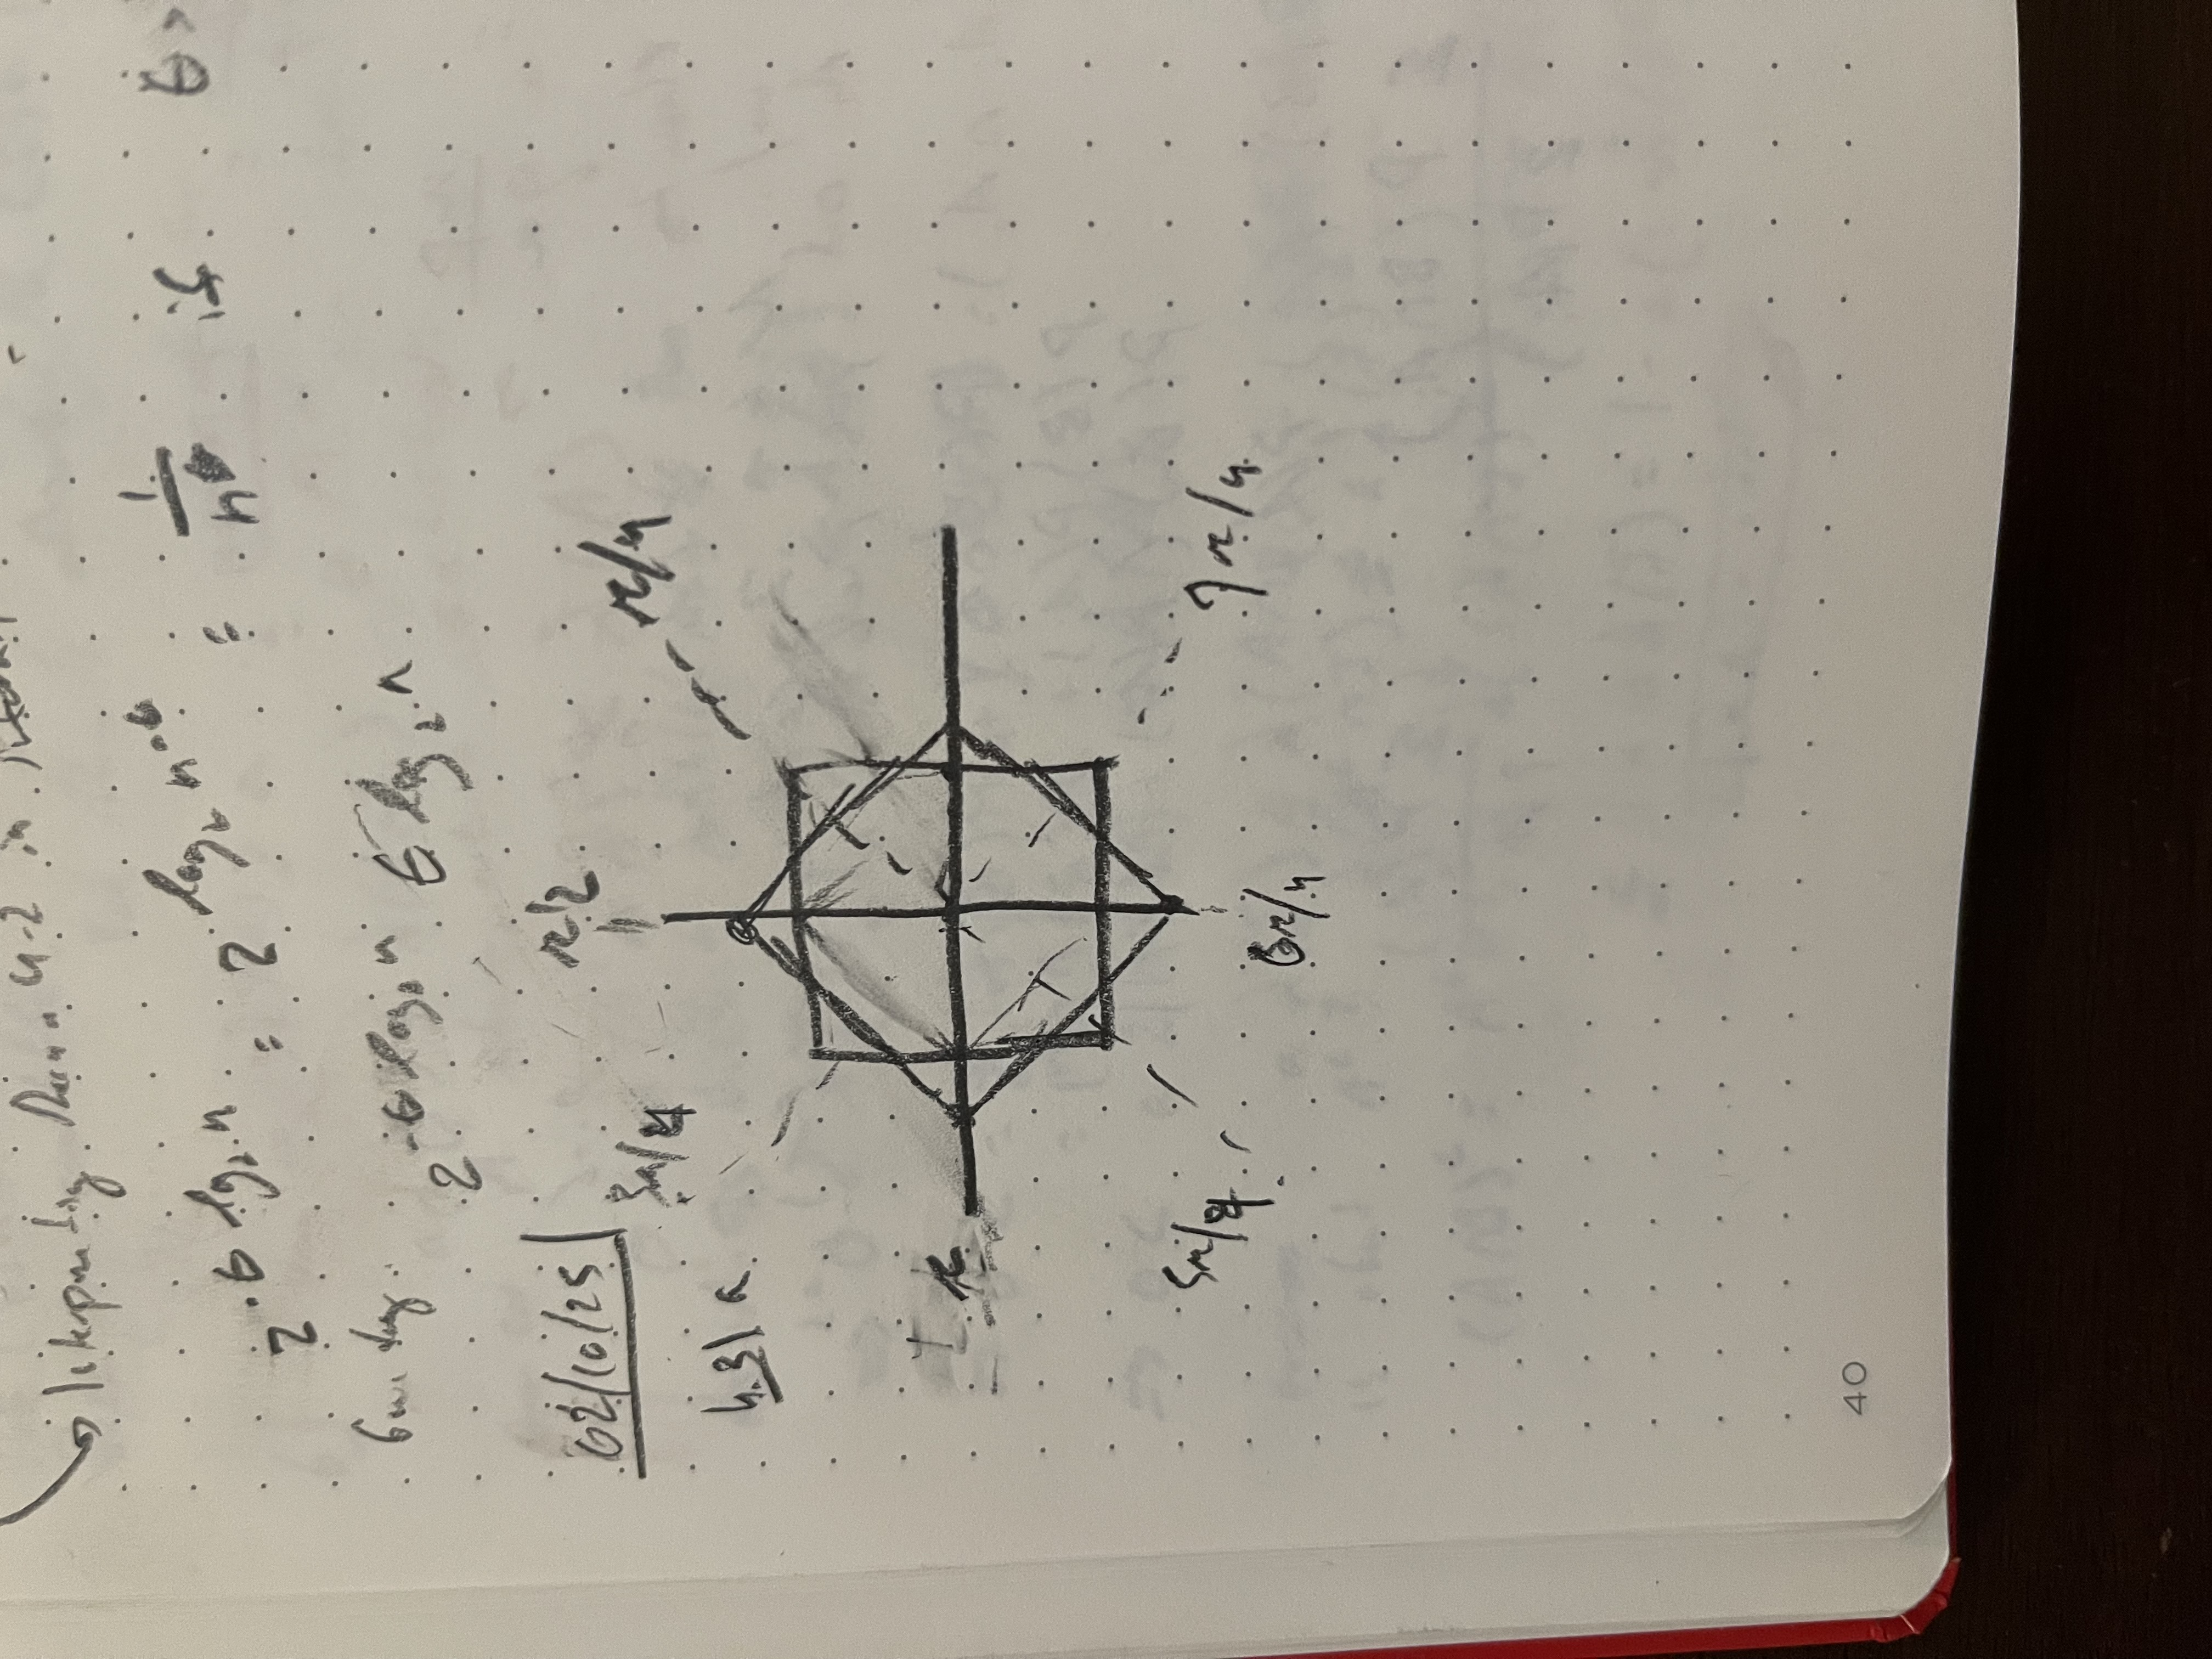
\includegraphics[angle=270, width=0.5\textwidth]{problem-4.3.a.jpg}
		\caption{Diagram for Question 4.3.a}
		\label{fig:example1}
	\end{figure} 
	\noindent Note that the $\limsup$ is the union of the two squares in the above picture, as any point that appears within one of the two squares will appear infinitely often. $\liminf$ is the intersection of the two squares - as only the points in the intersection will appear in every tail set.
	
	\item $\theta$ is rational. In this case:
	$$
		\text{angle}_n = 2\pi n * p/q = \frac{2p n\pi}{q}
	$$
	Note - we will have a picture like above, with cycle of $q$. Note that:
	$$
		A_{k} = A_{q + k} = A_{2q + k}
	$$
	For $k \in [q]$, as:
	$$
		\frac{2p (tq + k)\pi}{q} =
		2\pi pt + 2\pi \frac{pk}{q}
	$$
	Note that as $t$ and $p$ are integers, $2\pi pt$ is an integer multiple of $2\pi$, which just circles back to the angle of zero. And then, the added fraction of $ 2\pi \frac{pk}{q}$ is always the same. So, the union of the sets $A_k$ is the $\limsup$, like above, and the intersection is the $\liminf$, like above.
	
	\item $\theta$ is irrational. Note, in this case, we have that:
	$$
		\text{remainder } 2\pi n \theta / 2\pi
	$$
	Is dense in $[0,2\pi]$. Let's just assume that is the case for now. And so, take $x \not\in D$, where $D$ is the unit disk, but $x \in A_n$ for some $A_n$. Note, I think it might appear infinitely often in some $A_n$.
	\\\\
	Just making a leap here: but I think $\limsup A_n$ is the disk of radius $\sqrt{2}$, whereas $\liminf A_n$ is the disk of radius $1$. If you want to appear in every tail sequence - you have to be inside the unit disc.
		
\end{enumerate}

\subsubsection{4.7 Independence Complement Criteria} For events $A_1, \cdots, A_n$ consider the $2^n$ equations $P(B_1 \cap \cdots \cap B_n) = P(B_1) \cdots P(B_n)$ with $B_i = A_i$ or $B_i = A_i^c$ for each $i$. Show that $A_1, \cdots, A_n$ are independent if all these equations hold.
\\\\
We note a similar criteria that we have already approved - consider the $2^n$ equations $P(C_1 \cap \cdots \cap C_n) = P(C_1) \cdots P(C_n)$ with $C_i = A_i$ or $C_i = \Omega$ for each $i$. If each of these holds, then the $A_i$ are independent. We prove that if the $B$ equations hold, the $C$ equations holds. Thus, the $B$ equations also imply independence.
\\\\
First, assume one of the $C_i$ is $\Omega$. Thus, we have by countable additivity:
$$
	P(C_1 \cap \cdots \cap C_n) = 
	P(A_1 \cap \cdots \cap A_i \cap \cdots \cap A_n) + 
	P(A_1 \cap \cdots \cap A_i^c \cap \cdots \cap A_n)
$$
By the $B$ equations, the above equals:
$$
	= (P(A_i) + P(A_i)^c)(P(A_1) \cdots \widehat{P(A_i)} \cdots P(A_n)) =
	P(C_1) \cdots P(C_n)
$$
Now, we can take this result, and prove the equations hold for two $\Omega$ in the same way, and so on. Thus, we have that the $C_i$ equations hold if the $B_i$ equations hold, and the $B_i$ equations imply independence. Note, independence clearly implies the $B_i$ equations hold, so its an if and only if. qed.

\subsubsection{4.8 Class $\acal$ Partitions of $\Omega$} Recall that $\omega$ and $\omega'$ are called $\acal$ equivalent if, for every $A \in \acal$, $\omega$ and $\omega'$ lie either both in $A$ or both in $A^c$. That is:
$$
	I_A(\omega) = I_A(\omega') \quad\quad\quad A \in \acal
$$
This is clearly an equivalence relation, and this relation partitions $\Omega$. Note, there are $2^{|\acal|}$ possible equivalence classes - as for each $A \in \acal$, being in $A$ or $A^c$ defines two difference classes (note, this might not be entirely accurate if $\acal$ contains the complement or not. But, the idea is there). Also note - we proved that if $\omega$ and $\omega'$ are $\acal$ equivalent, then they are also $\sigma(\acal)$ equivalent.
\\\\
In this problem, we want to describe the $\acal$ partition for each of the following classes:
\begin{enumerate}
	\item The class of finite and cofinite sets. For this class - each $\omega$ would belong to a finite set of itself. And so, if $\omega' \neq \omega$, we would have $I_{\{\omega\}}(\omega) \neq I_{\{\omega\}}(\omega')$. The partition would be all singletons.
	
	\item The class of countable and cocountable sets. For this class - I again believe the partition would be the singletons. Say $\omega, \omega'$ both belong to a countable set $A$. Then, we have that $A - \{\omega'\}$ is also a countable set. In which case, $\omega$ and $\omega'$ are not in the same equivalence class.
	
	\item A partition (or arbitrary cardinality) of $\Omega$. So, each $A \in \acal$ is disjoint from the rest. We have that the $\omega \in A$ form an equivalence class - as $\omega,\omega' \in A$ also implies $\omega,\omega' \not\in B \in \acal$ for $B \neq A$.
	
	\item The level sets of $\sin(x)$, where $\Omega = \R$. Again, I believe this would form a partition of $\Omega$, as $\sin(x) = c$ has multiple $x$ that satisfy that value. If we want to describe the partitions - we have for $c \in [-1,1]$, the level set $L$ is:
	$$
		L = \{x \in \R : x = \arcsin(c) + 2n\pi \text{ or } x = \pi - \arcsin(c) + 2n\pi, n \in \Z\}
	$$
	Think of this in terms of the unit circle - $\arcsin(c)$ gives the $x$ value (angle value) on the positive $x$ axis. The $x$ value on the negative $x$ axis is symmetrical, or mirrored, which is given by $\pi - x$. This gives the set above.
	
	\item The $\sigma$ field in problem 3.5. In problem 3.5, we have $\Omega = \left\{(x,y) : 0 < x,y \leq 1\right\}$ is the unit square, and $\fcal$ is the class of sets of the form:
	$$
		\left\{(x,y) : x \in A, 0 < y \leq 1\right\}
	$$
	And let $P$ have value $\lambda(A)$ on this set. In the problem, we show that $(\Omega,\fcal,P)$ is a probability space. First, we note that $\fcal$ is a $\sigma$ algebra - as countable unions and intersections on the $x$ axis still remain within $\bcal$, and we still have all the ``height" from zero to one. We also clearly have $\Omega$ and complements. Probability measure still holds, as we still have countable additivity (if the $A$ are disjoint in $\bcal$, so are the corresponding sets above). It is also clear that for $A = \{(x,y) : 0 < x \leq 1, y = 1/2\}$, we have the outer measure $P^*(A) = 1$ while the inner measure $P^*(A) = 0$. That is essentially answering question 3.5.
	\\\\
	Now, we note that the $\acal$ partition of $\Omega$ is just straight lines $\{(x,y) : x \in (0,1], 0 < y \leq 1\}$. Every $\omega$ along such a line belongs to the same $A$ or $A^c$ for $A \in \fcal$ - this is because, each $A \in \fcal$ either contains the entire line, or it doesn't. Also, note that if $\omega$ and $\omega'$ are not on the same line - the singleton $\{x\}$ and $\{x'\}$ sets are within $\bcal$, so $\omega \in \{(x,y): 0 < y \leq 1\}$, but $\omega' \not\in \{(x,y): 0 < y \leq 1\}$. qed.
\end{enumerate}

\subsubsection{4.10 Independence does not imply Independent Information} Where by information, we mean which \textit{partition} of $\omega$ was selected. Note, some classes can be independent, but the information one class gives (ie, the partition that $\omega$ belongs to) might tell us which set in the other class the $\omega$ belongs to. This question essentially just emphasizes that the information notion is not altogether perfect.
\\\\
There is in the unit interval a set $H$ that is nonmeasurable in the extreme sense that its inner and outer Lebesgue measures are $0$ and $1$: $\lambda_*(H) = 0$ and $\lambda^*(H) = 1$. See problem 12.4 for its construction.
\\\\
\textbf{1.} Let $\Omega = (0,1]$, let $\gcal$ consist of the Borel sets in $\Omega$, and let $H$ be the set just described. Show that the class $\fcal$ of sets of the form $(H \cap G_1) \cup (H^c \cap G_2)$ for $G_1,G_2 \in \gcal$ is a $\sigma$ field, and that:
$$
	P\left[(H \cap G_1) \cup (H^c \cap G_2)\right] = \frac{1}{2}\lambda(G_1) + \frac{1}{2}\lambda(G_2)
$$
consistently defines a probability measure on $\fcal$. First, we show it is a $\sigma$ field. Clearly, it contains complements, as:
$$
	\left[(H \cap G_1) \cup (H^c \cap G_2)\right]^c =
	(H \cap G_1^c) \cup (H^c \cap G_2^c)
$$
Note $x \in (H \cap G_1^c) \implies x \not\in (H \cap G_1) \land x \not\in (H^c \cap G_2)$. Similar can be shown for $x \in (H^c \cap G_2^c)$, and so:
$$
	(H \cap G_1^c) \cup (H^c \cap G_2^c) \subseteq (H \cap G_1) \cup (H^c \cap G_2)
$$ 
Now, take $x \in \left[(H \cap G_1) \cup (H^c \cap G_2)\right]^c$. This implies $x \in H^c \lor x \in G_1^c$ \textit{and} $x \in H \lor x \in G_2^c$. If $x \in H^c$, then $x \not\in H$, in which case $x \in G_2^c$, and we have $x \in (H \cap G_2^c$. Similar for $x \in H$. Final case is $x \in G_1^c$ and $x \in G_2^c$, in which case $x \in H$ or $x \in H^c$. In all cases:
$$
	\left[(H \cap G_1) \cup (H^c \cap G_2)\right]^c \subseteq
	(H \cap G_1^c) \cup (H^c \cap G_2^c) 
$$
$$
	\implies
	\left[(H \cap G_1) \cup (H^c \cap G_2)\right]^c =
	(H \cap G_1^c) \cup (H^c \cap G_2^c)
$$
Note, see problem 2.7 for closed under countable unions (it is actually easier than the above. So yes, $\fcal$ is a $\sigma$ field. Now, we want to show that:
$$
	P\left[(H \cap G_1) \cup (H^c \cap G_2)\right] = \frac{1}{2}\lambda(G_1) + \frac{1}{2}\lambda(G_2)
$$
consistently defines a probability measure on $\fcal$. I will show that:
$$
	\lambda(G_1) = \lambda^*(G_1) = \lambda^*(H \cap G_1)
$$
First, by monotonicity of the outer measure, we have:
$$
	\lambda^*(H \cap G_1) \leq \lambda^*(G_1) \quad\quad\text{and}\quad\quad
	\lambda^*(H \cap G_1^c) \leq \lambda^*(G_1^c) = 1 - \lambda^*(G_1)
$$
Now, we note that as $G_1 \in \gcal = \bcal$, $G_1$ is measurable, and so:
$$
	\lambda^*(H \cap G_1) + \lambda^*(H \cap G_1^c) = \lambda^*(H) = 1 \implies
	\lambda^*(H \cap G_1) + 1 - \lambda^*(G_1) \geq 1
$$
$$
	\implies \lambda^*(H \cap G_1) \geq \lambda^*(G_1)
$$
Thus, we indeed have:
$$
	\lambda^*(H \cap G_1) = \lambda^*(G_1)
$$
We can similarly show:
$$
	\lambda^*(H \cap G_3) = \lambda^*(G_3)
$$
Given that $H \cap G_1 = H \cap G_3$, we thus must have:
$$
	\lambda(G_1) = \lambda(G_3)
$$
And similarly, we have $\lambda(G_2) = \lambda(G_4)$. Thus, we can conclude that:
$$
	(H \cap G_1) \cup (H^c \cap G_2) = (H \cap G_3) \cup (H^c \cap G_4) \implies
	\lambda(G_1) + \lambda(G_2) = \lambda(G_3) + \lambda(G_4)
$$
And the probability measure is consistent. Now, we note it is a probability measure, as it is clearly between $0$ and $1$, $P(\Omega) = 1$, and we have countable additivity (disjoint unions, transfer the disjoint unions into the $H \cap$ and $H^c \cap$ terms, and then rely on countable additivity of $\lambda$).
\\\\
\textbf{2.} Show that $P(H) = 1/2$ and that $P(G) = \lambda(G)$ for $G \in \gcal$. First, note that:
$$
	P(H) = P\left[(H \cap \Omega) \cup (H^c \cap \emptyset)\right] =
	1/2\lambda(\Omega) + 1/2\lambda(\emptyset) = 1/2
$$
Now, note that:
$$
	P(G) = P\left[(H \cap G) \cup (H^c \cap G)\right] =
	1/2\lambda(G) + 1/2\lambda(G) = \lambda(G)
$$
\textbf{3.} Show that $\gcal$ is generated by a countable subclass. Note, in problem 2.11, we showed that with the rational intervals, and that it contained the singletons.
\\\\
\textbf{4.} Show that $\gcal$ contains all the singletons and that $H$ and $\gcal$ are independent (in the sense that $\gcal$ is a class contained within $\fcal$). Above, we noted that $\gcal$ contains the singletons. Independence follows if for $G \in \gcal$, we have:
$$
	P(H \cap G) = P(H)P(G) = 1/2\lambda(G)
$$
Where the last equality is by part 3. Note that:
$$
	P(H \cap G) = P\left[(H \cap G) \cup (H^c \cap \emptyset)\right] = 1/2\lambda(G) + 1/2* 0 = 1/2\lambda(G)
$$
Thus, $H$ and $\gcal$ are independent.
\\\\
This construction proves the following: There exists a probability space $(\Omega, \fcal, P)$, a $\sigma$ field $\gcal$ in $\fcal$, and a set $H \in \fcal$, such that $P(H) = 1/2$, $H$ and $\gcal$ are independent, and $\gcal$ is generated by a countable subclass and contains all the singletons.
\\\\
This relates to example 4.10, in which, even though $\gcal$ and $H$ are independent, the ``information" contained in $G$ would tell us whether or not the drawn $\omega$ is in $H$ or not. However, note that with this example - the $\gcal$ is more \textit{natural} - it is countably generated, and contains singletons. In fact - it is the borel sets! However, the example involves the pathological set $H$, which throws everything for a loop.

\subsubsection{4.11 Different Criteria for $P(\limsup_n A_n) = 1$}
\begin{enumerate}
	\item If $A_1, A_2, \cdots$ are independent events, then prove:
	$$
		P\left(\bigcap_{n=1}^\infty A_n\right) = \prod_{n=1}^\infty P(A_n)
	$$
	And:
	$$
		P\left(\bigcup_{n=1}^\infty A_n\right) = 1 - \prod_{n=1}^\infty (1 - P(A_n))
	$$
	From these facts, derive the second Borel-Cantelli lemma by the well-known relation between infinite series and products (I would guess, it is the exponential fact).
	\\\\
	We note that for a finite sequence, independence implies:
	$$
		P\left(\bigcap_{n=1}^k A_n\right) = \prod_{n=1}^k P(A_n)
	$$
	We note that by continuity from above, we have:
	$$
		P\left(\bigcap_{n=1}^\infty A_n\right) = \prod_{n=1}^\infty P(A_n)
	$$
	We have by De'Morgan's laws, and independence implying independence of complements:
	$$
		P\left(\bigcup_{n=1}^\infty A_n\right) = 1 - P\left(\bigcap_{n=1}^\infty A_n^c\right) =
		1 - \prod_{n=1}^\infty (1 - P(A_n))
	$$
	Recall, the Borel Cantelli Lemma states that if $\{A_n\}$ is an independent sequence of events, and $\sum_n P(A_n)$ diverges, then $P(\limsup_n A_n) = 1$. Note, this follows if the complement of the $\limsup$ equals $0$, which follows if $\bigcap_{k=n}^\infty A_k^c = 0$ for all $n$. Note, we have $A_k^c$ are independent by above, and so:
	$$
		P\left(\bigcap_{k=n}^\infty A_k^c\right) = \prod_{k=n}^\infty (1 - P(A_k)) \leq
		\exp\left[-\sum_{k=n}^\infty P(A_k)\right] = 0
	$$
	As we know the sum diverges, and for $x \in [0,1]$, $(1-x) \leq \exp(-x)$. Note - the above is essentially just the proof for the second lemma, but made easier, as we don't have to apply a limit argument in the middle of the above steps, by the facts above. If we wanted to just \textit{derive} the lemma, then we might use the \href{https://en.wikipedia.org/wiki/Weierstrass_product_inequality?utm_source=chatgpt.com}{Weierstrass product inequality}. We have:
	$$
		1 - \sum_{n=1}^\infty P(A_n) \leq \prod_{n=1}^\infty (1 - P(A_n)) \leq \exp\left[-\sum_{n=1}^\infty P(A_n)\right]
	$$
	From this, we have:
	$$
		P\left(\bigcup_{n=1}^\infty A_n\right) = 1 - \prod_{n=1}^\infty (1 - P(A_n)) \geq
		1 - \exp\left[-\sum_{n=1}^\infty P(A_n)\right] = 1
	$$
	So, the probability of each union of $A_n$, and each tail sequence union of $A_n$, is $1$. Note, from this, we can derive $P(\limsup_n A_n) = 1$, as it is an intersection of unions of probability one. Note, that by itself isn't enough, but we can use continuity from above to prove it equals $1$ as well (as the unions each contain each other). qed.
	
	\item Show that $P(\limsup_n A_n) = 1$ if for each $k$ the series $\sum_{n > k} P(A_n | A_k^c \cap \cdots \cap A_{n-1}^c)$ diverges. From this deduce the second Borel-Cantelli lemma once again.
	\\\\
	Just from an informal ``information" level - the independent parts of each $A_n$, the probability of each $A_n$ when you are given the rest of the previous $A_k$ - diverges (note, I treat knowing $A_k^c$ equivalent to knowing $A_k$).
	\\\\
	Recall, we have:
	$$
		\limsup_n A_n = \bigcap_{n=1}^\infty \bigcup_{k=n}^\infty A_k
	$$
	As noted above, we can prove this probability equals one if each $\bigcup_{k=n}^\infty A_k$ equals one. Note - I think we can use the ratio test. If the limit of the ratios exists - then it must be greater than or equal to 1, as a ratio less than 1 would imply convergence. For the ratio test, we would have ratios of:
	$$
		\frac{P(A_k^c \cap \cdots \cap A_n^c \cap A_{n+1})}{P(A_k^c \cap \cdots \cap A_n^c)}
		\frac{P(A_k^c \cap \cdots \cap A_{n-1}^c)}{P(A_k^c \cap \cdots \cap A_{n-1}^c \cap A_n)}
	$$
	$$
		=
		\frac{P(A_k^c \cap \cdots \cap A_n^c \cap A_{n+1})}{P(A_k^c \cap \cdots \cap A_n^c)}
		\frac{P(A_k^c \cap \cdots \cap A_{n-1}^c \cap A_n^c) + P(A_k^c \cap \cdots \cap A_{n-1}^c \cap A_n)}{P(A_k^c \cap \cdots \cap A_{n-1}^c \cap A_n)}
	$$
	$$
		=
		\frac{P(A_k^c \cap \cdots \cap A_n^c \cap A_{n+1})}{P(A_k^c \cap \cdots \cap A_n^c)}
		\left(
		\frac{P(A_k^c \cap \cdots \cap A_{n-1}^c \cap A_n^c)}{P(A_k^c \cap \cdots \cap A_{n-1}^c \cap A_n)} + 1
		\right)
	$$
	I'm not sure if these ratios will actually help us.
	\\\\
	We will first derive the second Borel-Cantelli lemma, just to get something on the board. Assume that the $A_n$ are independent, and their sum diverges. Then, we have:
	$$
		\sum_{n > k} P(A_n | A_k^c \cap \cdots \cap A_{n-1}^c) = 
		\sum_{n > k} \frac{P(A_n \cap A_k^c \cap \cdots \cap A_{n-1}^c)}{P(A_k^c \cap \cdots \cap A_{n-1}^c)}
	$$
	$$
		=
		\sum_{n > k} \frac{P(A_n) P(A_k^c) \cdots P(A_{n-1}^c)}{P(A_k^c) \cdots P(A_{n-1}^c)} =
		\sum_{n > k} P(A_n) = \infty
	$$
	Where the $= \infty$ comes from every tail sequence diverging as well. Thus, we have that $P(\limsup_n A_n) = 1$, and this tail series fact is actually stronger. Now, we note, that $P(\limsup_n A_n) = 1$ if we have for every $k$:
	$$
		P\left[\bigcap_{n \geq k} A_n^c\right] = 0
	$$
	We use this fact in the original proof. Assume by contradiction that we have at least one $k$ such that the above is greater than $0$. Then, we note by assumption:
	$$
		\sum_{n > k} P(A_n | A_k^c \cap \cdots \cap A_{n-1}^c) = \infty
	$$
	$$
		\implies
		\sum_{n > k} P(A_n \cap A_k^c \cap \cdots \cap A_{n-1}^c) \frac{1}{P(A_k^c \cap \cdots \cap A_{n-1}^c)} = \infty
	$$
	Now, by contradiction, we have assumed:
	$$
		P\left[\bigcap_{n \geq k} A_n^c\right] = \epsilon > 0 \implies
		P(A_k^c \cap \cdots \cap A_{n-1}^c) \downarrow \epsilon
	$$
	Note, this implies the fraction approaches some constant $1/\epsilon$, and we can pull it out to conclude the first series diverges. More rigorously, for some $N$ large enough, for $n \geq N$, we have that:
	$$
		\epsilon \leq P(A_k^c \cap \cdots \cap A_{n-1}^c) \leq 2\epsilon
	$$
	Thus, on the tail, we find:
	$$
		\infty = \sum_{n > N} P(A_n \cap A_k^c \cap \cdots \cap A_{n-1}^c) \frac{1}{P(A_k^c \cap \cdots \cap A_{n-1}^c)} \geq
		2\epsilon \sum_{n > N} P(A_n \cap A_k^c \cap \cdots \cap A_{n-1}^c)
	$$
	$$
		\implies \sum_{n > k} P(A_n \cap A_k^c \cap \cdots \cap A_{n-1}^c) = \infty
	$$
	This is a contradiction, as we have each of the sets in the above sum are disjoint, and so their sum cannot be more than one. Thus, we must conclude for all $k$:
	$$
		P\left[\bigcap_{n \geq k} A_n^c\right] = 0 \implies
		P(\limsup_n A_n) = 1
	$$
	Note: I used help online to solve this. My problem was - I was too focused on directly proving it. I had gotten to the intersections equal 0/unions equal one statement - but direct proof was the problem. I think if I had pivoted quicker, I could have solved this one.
	
	\item Show by example that $P(\limsup_n A_n) = 1$ does not follow from the divergence of $\sum_n P(A_n | A_1^c \cap \cdots \cap A_{n-1}^c)$ alone.
	\\\\
	Thinking in terms of ``information" - I think this might follow if $A_1$ is a really \textit{small} event. Then, knowing $A_1^c$ might mean that you know \textit{a lot}, in which case the probabilities in the sum are large.
	\\\\
	Can't really figure this one out. First, we need $A_n$ to not be disjoint from the $A_k^c$ for $k < n$, as otherwise our conditional probabilities will be $0$. Then, we need $A_1^c$ to be restrictive enough so that the fraction becomes something like $x/x$, which is close to $1$. 
	
	\item Show that $P(\limsup_n A_n) = 1$ if and only if $\sum_n P(A \cup A_n)$ diverges for each $A$ of positive probability.
	\\\\
	Assume that $P(\limsup_n A_n) = 1$ and take $A$ such that $P(A) > 0$. Note, we have that:
	$$
		B_k = \bigcup_{i = k}^\infty A_i \implies 1 = P(\limsup_n A_n) =
		P\left(\bigcap_{n=1}^\infty B_n\right) \leq
		P(B_k)
	$$
	$$
		\implies P(B_k) = 1
	$$
	Assume by contradiction that $\sum_n P(A \cup A_n)$ converges. Then, for some $k$ large enough, we have for $\epsilon < P(A)$:
	$$
		P(A \cap B_k) = P\left(A \cap \bigcup_{i = k}^\infty A_i\right) =
		P\left(\bigcup_{i = k}^\infty A \cap A_i\right) \leq
		\sum_{i = k}^\infty P(A \cap A_i) < \epsilon 
	$$
	However, we note:
	$$
		P(A) = P((A \cap B_k) \cup (A \cap B_k^c)) = P(A \cap B_k) + P(A \cap B_k^c) = P(A \cap B_k)
	$$
	As $P(A \cap B_k^c) \leq P(B_k^c) = 0$. Thus, we have a contradiction, as we have found:
	$$
		P(A) = P(A \cap B_k) < \epsilon < P(A)
	$$
	And so, by contradiction, we have that $\sum_n P(A \cup A_n)$ diverges. Now, we go the other direction, and assume that the sum diverges for all $A$ with positive probability. We have $P(\limsup_n A_n) = 1$ if and only if $P(B_k) = 1$. By contradiction, assume that $P(B_k) < 1$, in which case $P(B_k) > 1$. Then, we have:
	$$
		\sum_{i=k}^\infty P(B_k^c \cap A_i) \text{ diverges} \implies
		\sum_{i=k}^\infty P(A_i - B_k) \text{ diverges}
	$$
	$$
		\implies
		\sum_{i=k}^\infty P(A_i - (A_k \cup \cdots \cup A_{i-1})) \text{ diverges}
	$$
	Note, the last step is because $A_k \cup \cdots \cup A_{i-1} \subseteq B_k$. Now, note that the above is a summation of disjoint sets, and so, we have:
	$$
		\implies
		P\left(\bigcup_{i=k}^\infty A_i - (A_k \cup \cdots \cup A_{i-1})\right) = \infty
		\implies
		P(B_k) = \infty
	$$
	This is a contradiction, as an event must have less than or equal to $1$ probability. And so, by contradiction, we have that $P(B_k) = 1$ and thus $P(\limsup_n A_n) = 1$. qed.
	
	\item If sets $A_n$ are independent and $P(A_n) < 1$ for all $n$, then $P(A_n \io) = 1$ if and only if $P(\bigcup_n A_n) = 1$.
	\\\\
	We first go in the easy direction. Note, $P(A_n \io) = 1$ if and only if $P(B_k) = 1$ for all $k$. Note, for $k = 1$, we have:
	$$
		1 = P(B_1) = P\left(\bigcup_n A_n\right)
	$$
	And so now, we go in the other direction. Recall, one sufficient condition for $P(A_n \io) = 1$ is that:
	$$
		P\left(\bigcap_{i=k} A_i^c\right) = 0
	$$
	For all $i$. Note, we have by assumption:
	$$
		P\left(\bigcap_{i=1} A_i^c\right) = 0
	$$
	As the $A_i^c$ are independent events as well, by part $a$, we have:
	$$
		P\left(\bigcap_{i=k} A_i^c\right) = \prod_{i=k}^\infty P(A_i^c)
	$$
	For $j = 1, \cdots, k-1$, we note that $P(A_j) < 1$, and so we have that $P(A_j^c) > 0$. And so, we have that:
	$$
		0 = P\left(\bigcap_{i=1} A_i^c\right) =
		\lim_{n \to \infty} \prod_{i=1}^n P(A_i^c) =
		P(A_1^c) \cdots P(A_{k-1}^c) \lim_{n \to \infty} \prod_{i=k}^n P(A_i^c)
	$$
	$$
		\implies
		0 = P(A_1^c) \cdots P(A_{k-1}^c) P\left(\bigcap_{i=k} A_i^c\right)
	$$
	As $P(A_1^c) \cdots P(A_{k-1}^c) > 0$, we must have for all $k$:
	$$
		0 = P\left(\bigcap_{i=k} A_i^c\right) \implies P(A_n \io) = 1
	$$
	Thus, we can indeed conclude that if sets $A_n$ are independent and $P(A_n) < 1$ for all $n$, then $P(A_n \io) = 1$ if and only if $P(\cup_n A_n) = 1$. qed.
\end{enumerate}

\subsubsection{4.14 Infinite Independent Events Criteria for a Nonatomic Space} Suppose that there are in $(\Omega, \fcal, P)$ independent events $A_1, A_2, \cdots$ such that, if:
$$
	\alpha_n = \min\left\{P(A_n), 1 - P(A_n)\right\}
$$
Then $\sum \alpha_n = \infty$. Show that $P$ is \textit{nonatomic}. 
\\\\
Recall - nonatomic means that if $P(A) > 0$, there exists a $B$ such that $B \subset A$ and $0 < P(B) < P(A)$, and $A,B \in \fcal$. Note, in problem 2-19, we prove that $\bcal$ is nonatomic with the lebesgue measure (deriving a contradiction from a single point needing to have $0$ lebesgue measure). We also showed that in the nonatomic case, that for $0 \leq x \leq P(A)$, there exists a $B$ such that $B \subset A$ and $P(B) = x$. Finally, we proved that if $p_1, p_2, \cdots$ are nonnegative and add to $1$, then $A$ can be decomposed into sets $B_1, B_2, \cdots$ such that $P(B_n) = p_nP(A)$.
\\\\
Take an $A \in \fcal$. We just have to show that there is a $B$ such that $B \subset A$, and $0 < P(B) < P(A)$ and $B \in \fcal$. Take $B_i$ as either $A_i$ or $A_i^c$, whichever satisfies $P(B_i) = \alpha_i$. Note, by Borel-Cantelli, we have $P(B_i \io) = 1$, and by 4.11e, we have:
$$
	P(\cup_i B_i) = 1
$$
Examine each $A \cap B_i$. We note for some $B_i$, we have that $0 < P(A \cap B_i) < P(A)$, and thus $(\Omega,\fcal,P)$ is nonatomic. First, note they all can't be zero, as that would imply:
$$
	0 = P(A \cap B_i) \implies
	0 = P(\cup A \cap B_i) = P(A \cap \cup B_i) = P(A)
$$
Which is a contradiction. Note, the only thing to do now is prove that if $P(A \cap B_i) > 0$, we don't have $P(A \cap B_i) = P(A)$. However, this could be the case - what if the $B_i$ are disjoint, and $A = B_j$. This path will not work.
\\\\
\textbf{Attempt 2} Using the solution at the back of the book. First, note that:
$$
	\lim_{n \to \infty} \max P(B_1 \cap \cdots \cap B_n) = 0
$$
Here, we take $B_i$ as either $A_i$ or $A_i^c$ - note, we have:
$$
	P(B_1 \cap \cdots \cap B_n) = \prod_{i=1}^n P(B_i) \leq \exp\left(-\sum_{i=1}^n P(B_i)\right)
$$
Note, no matter the sum, it always diverges, and so yes, the limit is indeed $0$, even if you take the maximizing $B_i$. Now, define:
$$
	C_x = \left[\omega: \sum_n I_{A_n}(\omega) 2^{-n} \leq x\right]
$$
First note, $C_x$ contains all $\omega$ not in the $A_n$. Then, it would pick up the $\omega$ that appear sporadically, or in tail sequences far away enough such that the sum of the corresponding $2^{-n}$ does not exceed $x$. We want to show that:
$$
	P(A \cap C_x)
$$
Is continuous in $x$. Note that the above is maximized for $x = 1$, in which case $P(A \cap C_1) = P(A)$, as $C_1 = \Omega$, and minimized for $x = 0$, in which case $P(A \cap C_0) = P\left(A \cap \left(\cup A_i\right)^c\right) = 0$, as we have $P(\cup A_i) = 1$, and so its complement has probability zero. We want to show it is continuous in $x$. So, take some $c \in (0,1)$. We want to show that as $x_n \to c$, we have:
$$
	\lim_n P(A \cap C_{x_n}) = P(A \cap C_c)
$$
I believe this can be done by looking at the symmetric difference:
$$
	(A \cap C_{x_n}) \triangle (A \cap C_c)
$$
And noting that for $x_n$ close enough to $c$, the $\omega$ in one of the sets but not the other must be contained within small enough dyadic intervals. Or, we can make use of the fact that the maximum goes to $0$. We first assume that $x_n \uparrow c$. Later, we will generalize the argument for all $x_n \to c$. Note, in this case, we have:
$$
	A \cap C_{x_n} \subseteq A \cap C_c \implies
	P(A \cap C_c) - P(A \cap C_{x_n}) = 
	P(A \cap C_c - A \cap C_{x_n})
$$
$$
	= P(A \cap (C_c - C_{x_n})) \leq
	P(C_c - C_{x_n})
$$
So, we examine:
$$
	\omega \in C_c - C_{x_n}
$$
Note, $x_n$ can be arbitrarily close to $c$, and so $\omega \in C_c - C_{x_n}$ implies:
$$
	c - \epsilon \leq \sum_n I_{A_n}(\omega)2^{-n} \leq c
$$
Note, $c$ has at most two dyadic expansions (terminating and non-terminating):
$$
	c = \sum_n d^1_n(c)2^{-n} =
	\sum_n d^2_n(c)2^{-n}
$$
If $\epsilon < 2^{-k}$, we have that $\omega$ must satisfy for $n = 1, \cdots, k-1$:
$$
	\forall n \,\,\, I_{A_n}(\omega) = d^1_n(c) \text{ or } \forall n \,\,\, I_{A_n}(\omega) = d^2_n(c)
$$
If $\omega$ doesn't satisfy either of the two above equations, then the difference:
$$
	\left|\sum_n d^i_n(c)2^{-n} - \sum_n I_{A_n}(\omega)2^{-n}\right| > 2^{-k} > \epsilon
$$
Note, by the fact that for any \textit{specific} choice of $B_i$, we have:
$$
	\lim_{n \to \infty} \max P(B_1 \cap \cdots \cap B_n) = 0
$$
We thus have that:
$$
	\lim_{n \to \infty} P(C_c - C_{x_n}) \leq
	\lim_{n \to \infty} P(B^1_1 \cap \cdots \cap B^1_n) + P(B^2_1 \cap \cdots \cap B^2_n) = 0
$$
And so, for $x_n \uparrow c$, we indeed have:
$$
	\lim_n |P(A \cap C_c) - P(A \cap C_{x_n})| = \lim_n P(A \cap C_c) - P(A \cap C_{x_n}) \leq \lim_{n \to \infty} P(C_c - C_{x_n}) \leq 0
$$
$$
	\implies \lim_n P(A \cap C_{x_n}) = P(A \cap C_c)
$$
Now, for $x_n \to c$. Note, we can still prove that:
$$
	\lim_n |P(A \cap C_c) - P(A \cap C_{x_n})| = 0
$$
As either $A \cap C_c \subseteq A \cap C_{x_n}$, or vice versa, and we can still apply the argument for the bigger interval $(c-\epsilon,c+\epsilon)$ to conclude that the $\omega \in (A \cap C_{x_n}) \triangle (A \cap C_c)$ have to be in one of two specific sequences of $B_i$, which both have probability $0$. Thus, we indeed have that:
$$
	P(A \cap C_x)
$$
Is continuous in $x$. Thus, we can conclude there is some $x$ such that:
$$
	0 < P(A \cap C_x) < P(A)
$$
We clearly have $A \cap C_x \subseteq P(A)$. So, the final thing to note is that $A \cap C_x \in \fcal$, which comes from $C_x \in \fcal$. Note, the function describing $C_x$ can be shown to be a measurable mapping, in which case the preimage of an interval $[0,x]$ would be a measurable set as well. Note, clearly each partial sum is a measurable mapping (as the preimage is clearly measurable), and thus the infinite sum is measurable as well. This actually gives us a way to directly prove $C_x$ is measurable. First, note that for:
$$
	C^k_x = \left[\omega: \sum_{n=1}^k I_{A_n}(\omega) 2^{-n} \leq x\right]
$$
We have that $C^k_x$ is clearly measurable. There are certain sequences of $x \in B_1 \cap \cdots \cap B_k$, where $B_i = A_i$ or $A_i^c$, that satisfy the above equation. One such example is $x \in A_1^c \cap \cdots \cap A_k^c$. So, $C^k_x \in \fcal$, as $C^k_x$ is a finite union of finite intersections of measurable $B_i$. Now, we have that:
$$
	C_x = \bigcap_{k=1}^\infty C^k_x
$$
Clearly, $\omega \in C^k_x \implies \omega \in C_x$, as we can just take $\omega \in A_i^c$ for $i > k$. Now, take $\omega \in C_x$. We note that $\omega$ must be in $B_1, \cdots, B_k$ such that the sum satisfies:
$$
	\sum_{n=1}^k I_{A_n}(\omega) 2^{-n} \leq x
$$
Given that the infinite sum also satisfies being less than $x$. And so, $\omega \in C_x \implies \omega \in C^k_x$ for all $k$. Thus, we have that $C_x$ is a countable intersection of $\fcal$ sets, and so $C_x$ is within $\fcal$.
\\\\
Thus, we have proved that if there are in $(\Omega, \fcal, P)$ independent events $A_1, A_2, \cdots$ such that for:
$$
	\alpha_n = \min\left\{P(A_n), 1 - P(A_n)\right\}
$$
Then $\sum \alpha_n = \infty$, we have that $P$ is \textit{nonatomic}. qed.

\subsubsection{4.15 Density of the Square-Free Integers} Let $F$ be the set of square-free integers - those integers not divisible by any perfect square. Let $F_l$ be the set of $m$ such that $p^2|m$ ($p^2$ divides $m$) for no $p \leq l$, and show that $D(F_l) = \prod_{p \leq l}(1-p^{-2})$. Show that $P_n(F_l - F) \leq \sum_{p > l} p^{-2}$, and conclude that the square-free integers have density:
$$
	\prod_p (1-p^{-2}) = 6/\pi^2
$$
We need to recall a lot of the above notation. Its all from problem 2.18. We have that:
$$
	P_n(A) = \frac{1}{n}\#\left\{m : 1 \leq m \leq n, m \in A\right\}
$$
We also have that $P_n$ is a \textit{discrete} probability measure on $\Omega = \{1, 2, \cdots\}$. We define the \textit{density} as:
$$
	D(A) = \lim_n P_n(A)
$$
We first want to show:
$$
	D(F_l) = \prod_{p \leq l}(1-p^{-2})
$$
Note - I will first go with the assumption that $p$ is \textit{prime}. Note, assuming prime makes things easier, as we have that $lcm(p_1,p_2) = p_1p_2$, and we similarly have $lcm(p_1^2,p_2^2) = p_1^2p_2^2$. Further, in problem 2.18 (which this problem seems to be a continuation of), $p$ referred to prime numbers as well.
\\\\
We recall the notation that $M_a = \{ak: k = 1, 2, \cdots\}$. These are periodic sets, and in problem 2.18, we proved the following (note, it should also be intuitively clear):
$$
	P_n(M_a) = \frac{1}{n}\floor{\frac{n}{a}} \to \frac{1}{a} = D(M_a)
	\quad\quad\quad
	M_a \cap M_b = M_{lcm(a,b)}
$$
We clearly have:
$$
	F_l = \left[\bigcup_{p \leq l} M_{p^2}\right]^c \implies
	F_l = \bigcap_{p \leq l} M_{p^2}^c
$$
We now note that for prime $p_1, \cdots, p_k$, we have that:
$$
	P_n\left[M_{p_1^2} \cap \cdots \cap M_{p_k^2}\right] =
	P_n\left[M_{lcm(p_1^2, \cdots, p_k^2)}\right] =
	P_n\left[M_{p_1^2 \cdots p_k^2}\right] =
	\frac{1}{n}\floor{\frac{n}{p_1^2 \cdots p_k^2}} \to 
	\frac{1}{p_1^2 \cdots p_k^2}
$$
So, we now find:
$$
	D(F_l) = 
	\lim_{n \to \infty} P_n(F_l) =
	1 - \lim_{n \to \infty} P_n\left(\bigcup_{p \leq l} M_{p^2}\right)
$$
We now make use of the inclusion-exclusion principle to find the above equals:
$$
	1 - 
	\lim_{n \to \infty} \sum_{1 < p_1 \leq l} P_n\left(M_{lcm(p_1^2)}\right) +
	\lim_{n \to \infty} \sum_{1 < p_1 < p_2 \leq l} P_n\left(M_{lcm(p_1^2,p_2^2)}\right) + \cdots
$$
$$
	+ (-1)^k \lim_{n \to \infty} \sum_{1 < p_1 < p_2 < \cdots < p_k \leq l} 
	P_n\left(M_{lcm(p_1^2,p_2^2, \cdots, p_k^2)}\right)
$$
$$
	=
	1 -
	\sum_{1 < p_1 \leq l} \frac{1}{p_1^2} +
	\sum_{1 < p_1 < p_2 \leq l} \frac{1}{p_1^2p_2^2} + \cdots +
	(-1)^k \sum_{1 < p_1 < p_2 < \cdots < p_k \leq l} \frac{1}{p_1^2 \cdots p_k^2}
$$
$$
	= (1-p_1^2)(1-p_2^2) \cdots (1-p_k^2)
$$
Where the final equality is a well known formula for the multiplication of $(1-p_i)$ terms. (also called the inclusion-exclusion principle). The second inequality is making use of our limit fact proved above. Thus, we indeed have:
$$
	D(F_l) = \prod_{p \leq l}(1 - p^{-2})
$$
Now, the task is to show that $P_n(F_l - F) \leq \sum_{p > l} p^{-2}$. We note that:
$$
	F_l - F \subseteq \bigcup_{p > l} M_{p^2}
$$
Take $x \in F_l - F$. We have that $x$ is \textit{not} divisible by $p^2$ for $p \leq l$, but $x$ is divisible by some $y^2$, as $x \not\in F$. Note, $y^2$ has a prime factorization:
$$
	y = \prod_{t=1}^k p_t \implies
	y^2 = \prod_{t=1}^k p_t^2
$$
Note, these $p_t^2$ must divide $x$. However, we cannot have $p_t \leq l$ by $x \in F_l$, and so we must have $p_t > l \implies x \in M_{p^2}$. Thus, we find by the above results and subadditivity:
$$
	P_n(F_l - F) = P_n\left(\bigcup_{p > l} M_{p^2}\right) \leq
	\sum_{p > l} M_{p^2} = \sum_{p > l} \frac{1}{n}\floor{\frac{n}{p^2}} \leq
	\sum_{p > l} p^{-2}
$$
Thus, we can indeed conclude that:
$$
	P_n(F_l - F) \leq \sum_{p > l} p^{-2}
$$
Finally, we want to conclude that:
$$
	D(F) = \prod_p (1 - p^{-2})
$$
Note, we have:
$$
	0 \leq P_n(F_l) - P_n(F) = P_n(F_l - F)
$$
Note, the final term has an inequality that does not depend on $n$, and so we have:
$$
	0 \leq P_n(F_l) - P_n(F) \leq \sum_{p > l} p^{-2}
$$
As limits maintain boundedness, we find, taking a limit to $n$ on the middle term:
$$
	0 \leq D(F_l) - D(F) \leq \sum_{p > l} p^{-2}
$$
Finally, we note the well known result that $\sum_n \frac{1}{n^2}$ converges, and so for $l \to \infty$, we have the right hand sum goes to $0$. Thus, we have:
$$
	0 \leq \lim_{l \to \infty} D(F_l) - D(F) \leq 0 \implies
	D(F) = \lim_{l \to \infty} D(F_l)
$$
$$
	\implies
	D(F) = \prod_p (1 - p^{-2})
$$
The final point is an equality that $\prod_p (1 - p^{-2}) = 6/\pi^2$. I will note prove this here. qed.

\section{Section 5 - Simple Random Variables}
\subsection{Notes}
\subsubsection{Simple Random Variables Definitions}
\paragraph{Definition - Simple Random Variable} Let $X$ be a real-valued function on $\Omega$ for the arbitrary probability space $(\Omega,\fcal,P)$. $X$ is a \textit{simple random variable} if it has finite range (ie, takes on finitely many values) and if:
$$
	\left[\omega : X(\omega) = x\right] \in \fcal
$$
For each real $x$. Note, the above set is $\emptyset$ for each $x \in \R$ that is not in the range. It is also customary to omit the $\omega$ function input, ie, just call it the simple random variable $X$. We also have the customary shorthand of:
$$
	\left[X = x\right] = \left[\omega : X(\omega) = x\right]
$$
Some examples include the $n$ dyadic digit, $d_n(\omega)$ (which takes on finite values of $0$ and $1$). The run lengths $l_n(\omega)$ of zeros starting at $n$ are \textit{not} simple random variables, as they take on a countable number of values. A finite sum:
$$
	X = \sum_i x_i I_{A_i}
$$
Is a random variable if the $A_i$ form a partition of $\Omega$ into $\fcal$ sets. Moreover, we can take $A_i = [X = x_i]$, and express a simple random variable $X$ as a finite indicator sum. Note, however - this is not a \textit{unique} representation, as we can have $A_{ij}$ forming a partition of $A_i$.

\paragraph{Definition - Measurable with Respect to a Sub-$\sigma$-field} If $\gcal$ is a sub-$\sigma$-field of $\fcal$, a simple random variable $X$ is \textit{measurable $\gcal$}, or \textit{measurable with respect to $\gcal$}, if $[X = x] \in \gcal$ for each $x$. By definition, a simple random variable is always measurable $\fcal$. Since:
$$
	[X \in H] = \bigcup [X = x]
$$
Where the union extends over the finitely many $x \in H$ and $x \in range(X)$, we have that $[X \in H] \in \gcal$ for every $H \subset \R$ if $X$ is a simple random variable measurable $\gcal$ (as finite unions stay within $\gcal$).

\paragraph{Definition - $\sigma$ field generated by a simple random variable $X$} The $\sigma$ field $\sigma(X)$ \textit{generated} by $X$ is the smallest $\sigma$ field with respect to which $X$ is measurable; that is $\sigma(X)$ is the intersection of all $\sigma$ fields with respect to which $X$ is measurable. For a finite or infinite sequence $X_1, X_2, \cdots$ of simple random variables, $\sigma(X_1, X_2, \cdots)$ is the smallest $\sigma$ field with respect to which each $X_i$ is measurable.

\paragraph{Theorem 5.1 - Simple Random Variable Generated $\sigma$ Fields and Function of Simple Random Variables} Let $X_1, \cdots, X_n$ be simple random variables.
\begin{enumerate}
	\item The $\sigma$ field $\sigma(X_1, \cdots, X_n)$ consists of the sets:
	$$
		\left[(X_1, \cdots, X_n) \in H\right] =
		\left[\omega : (X_1(\omega), \cdots, X_n(\omega)) \in H\right]
	$$
	For $H \subset \R^n$. $H$ in this representation may be taken finite (by taking the intersection of $H$ and the finite amount of possible coordinates by the SRVs $X_i$).
	
	\item A SRV $Y$ is measurable $\sigma(X_1, \cdots, X_n)$ if and only if:
	$$
		Y = f(X_1, \cdots, X_n)
	$$
	for some $f: \R^n \to \R$. 
\end{enumerate}

\paragraph{Proof of Theorem 5.1}
\begin{enumerate}
	\item We start with part (1). Let $\mcal$ be the class of sets of the form $\left[(X_1, \cdots, X_n) \in H\right]$. Note that sets of the form:
	$$
		\left[(X_1, \cdots, X_n) = (x_1, \cdots, x_n)\right] =
		\bigcap_{i=1}^n [X_i = x_i] \in \sigma(X_1, \cdots, X_n)
	$$
	As $X_i$ is measurable with respect to $\sigma(X_1, \cdots, X_n)$, we have that $[X_i = x_i] \in \sigma(X_1, \cdots, X_n)$, and a $\sigma$ algebra would contain a finite intersection. Note that each set in $\mcal$ is a finite union of sets of the above form - for all coordinates in the range of the tuple that are within $H$. And so, we have:
	$$
		\mcal \subseteq \sigma(X_1, \cdots, X_n)
	$$
	Now, we go the other direction. Note that $\mcal$ is a $\sigma$ field. We have $\Omega = [(X_1, \cdots, X_n) \in \R^n] \in \mcal$, $[(X_1, \cdots, X_n) \in H]^c = [(X_1, \cdots, X_n) \in H^c] \in \mcal$, and:
	$$
		\bigcup_j [(X_1, \cdots, X_n) \in H_j] = [(X_1, \cdots, X_n) \in \bigcup_j H_j] \in \mcal
	$$
	Note that each $X_i$ is measurable with respect to $\mcal$. This is because:
	$$
		[X_i = x] = [(X_1, \cdots, X_i, \cdots, X_n) \in \R \times \cdots \times x \times \cdots \times \R] \in H
	$$
	Thus, $\mcal$ is a $\sigma$ field with respect to which each $X_i$ is measurable, and so we have:
	$$
		\sigma(X_1, \cdots, X_n) \subseteq \mcal \implies
		\mcal = \sigma(X_1, \cdots, X_n)
	$$
	
	\item Assume that $Y$ is a function of the $X_1, \cdots, X_n$:
	$$
		Y = f(X_1, \cdots, X_n)
	$$
	Note that:
	$$
		[Y = y] = [(X_1, \cdots, X_n) = (x_1, \cdots, x_n) : f(x_1, \cdots, x_n) = y]
	$$
	Note - $[Y = y] \in \sigma(X_1, \cdots, X_n)$, if we let $H = [(x_1, \cdots, x_n) : f(x_1, \cdots, x_n) = y]$. One confusion I had is - what if a coordinate $(x_1, \cdots, x_n)$ that maps to $y$ cannot be achieved by $(X_1, \cdots, X_n)$ (ie, it is not in the range?). Note, this means for no $\omega$, $[Y = y]$ via that coordinate mapping, as for all $\omega$, $Y = f(X_1, \cdots, X_n)$. So, it is consistent.
	\\\\
	Now, we assume that $Y$ is measurable $\sigma(X_1, \cdots, X_n)$. Let $y_1, \cdots, y_r$ be the distinct values $Y$ assumes. By part (1), there exist sets $H_1, \cdots, H_r$ in $\R^n$ such that:
	$$
		[\omega: Y(\omega) = y_i] = [\omega: (X_1(\omega), \cdots, X_n(\omega)) \in H_i]
	$$
	Define $f = \sum_{i=1}^r y_i I_{H_i}$. Note, $H_i$ and $H_j$ are not disjoint only if $y_i = y_j$. Therefore, the $H_i$ partition $\R^n$, and each $(X_1(\omega), \cdots, X_n(\omega))$ lies in exactly one of the $H_i$, and it follows that:
	$$
		Y(\omega) = f(X_1(\omega), \cdots, X_n(\omega))
	$$
	Thus, a simple random variable $Y$ is measurable $\sigma(X_1, \cdots, X_n)$ if and only if $Y$ can be written as a function of the $X_1, \cdots, X_n$. qed.
\end{enumerate}
Note: By the above theorem, it follows that functions of simple random variables are again simple random variables (as the function would be measurable $\fcal$, and the function could only take on finite values). Thus, $X^2$, $e^{tX}$, and so on are simple random variables along with $X$. Taking $f$ to be:
$$
	\sum_{i=1}^n x_i \quad\quad\quad
	\prod_{i=1}^n x_i \quad\quad\quad
	\max_{i \leq n} x_i
$$
Shows that sums, products, and maxima of simple random variables are again simple random variables. What is key in all of this is the finiteness - note that each function can still only take on a finite number of values.

\paragraph{Example 5.2} Let $s_n(\omega) = \sum_{k=1}^n r_k(\omega)$ be the partial sums of the Rademacher functions. By Theorem 5.1ii, $s_k$ is measurable $\sigma(r_1, \cdots, r_n)$ for $k \leq n$. And $r_k = s_k - s_{k-1}$ is measurable $\sigma(s_1, \cdots, s_n)$. Thus:
$$
	\sigma(r_1, \cdots, r_n) = \sigma(s_1, \cdots, s_n)
$$
In information terms, this means that the first $n$ positions of a random walk contain the same information as the first $n$ distances moved. Or, knowing the first $n$ fortunes of the gambler is the same as knowing his gains and losses on each of the first $n$ plays.

\subsubsection{Convergence of Simple Random Variables}
A common problem for probability is: for given random variables $X$ and $X_1, X_2, \cdots$ on a probability space $(\Omega,\fcal,P)$, look for the probability of the event that:
$$
	\lim_n X_n(\omega) = X(\omega)
$$
The normal number theorem is essentially concerned with $X_n(\omega) = n^{-1}\sum_{i=1}^n d_i(\omega)$ and $X(\omega) = 1/2$, as an example. It is easy and convenient to characterize the complementary event: $X_n(\omega)$ \textit{fails} to converge to $X(\omega)$ if and only if there is some $\epsilon$ such that for no $m$, does $|X_n(\omega) - X(\omega)|$ remain below $\epsilon$ for all $n$ exceeding $m$. That is to say, if and only if, for some $\epsilon$, $|X_n(\omega) - X(\omega)| \geq \epsilon$ holds for infinitely many values of $n$. Therefore:
$$
	\left[\lim_n X_n = X\right]^c = \bigcup_\epsilon \left[|X_n - X| \geq \epsilon \;\io\right]
$$
The union can be restricted to rational (positive) $\epsilon$ because the set in the union \textit{increases} as $\epsilon$ \textit{decreases} (ie, for any positive $\epsilon$, we can find $1/n$ rational that is smaller, and all $\omega$ will be included).
\\\\
Note, this implies that the event $\left[\lim_n X_n = X\right]$ always lies within the basic $\sigma$ field $\fcal$. First note, $\left[|X_n - X| \geq \epsilon\right] \in \fcal$. We have that $Y = |X_n - X|$ is a simple random variable on $\fcal$, and restricting the set greater than $\epsilon$ is in the field (note, this section for some reason seems to be agnostic to whether the rv is \textit{simple} or not - in this case, we still have functions of rvs are rvs (measurable), and so to is the inequality). As $\io$ is a countable intersection of countable unions, the $\io$ terms in the countable union are within $\fcal$, and as complements stay in $\fcal$, we indeed have that $\left[\lim_n X_n = X\right] \in \fcal$. This event has probability 1 if and only if:
$$
	P\left[|X_n - X| \geq \epsilon \;\io\right] = 0
$$
For each $\epsilon$. Note, by Theorem 4.1, we have the above implies:
$$
	0 \leq \liminf_n P\left[|X_n - X| \geq \epsilon\right] \leq
	\limsup_n P\left[|X_n - X| \geq \epsilon\right] \leq
	P\left[|X_n - X| \geq \epsilon \;\io\right] = 0
$$
$$
	\implies
	\lim_n P\left[|X_n - X| \geq \epsilon\right] = 0
$$

\paragraph{Definition: Convergence in Probability} The above argument leads to a definition: If $\lim_n P\left[|X_n - X| \geq \epsilon\right] = 0$ holds for each positive $\epsilon$, then $X_n$ is said to \textit{converge to $X$ in probability}, written $X_n \to_p X$. These arguments prove the following theorem:

\paragraph{Theorem 5.2 - Convergence with Probability 1, and Convergence in Probability}
\begin{enumerate}
	\item There is convergence $\lim_n X_n = X$ with probability 1 if and only if $P\left[|X_n - X| \geq \epsilon \;\io\right] = 0$ holds for each $\epsilon$.
	
	\item Convergence with probability 1 implies convergence in probability.
\end{enumerate}
Go back to the normal number theorem - it dealt with \textit{convergence with probability 1}, as we ultimately said something along the lines of, the complement had probability $0$. However, Theorem 1.1 had to do with convergence in probability of the same sequence. By Theorem 5.2 - we should have that Theorem 1.1 (the weak law of large numbers) is a consequence of the normal number theorem. Note, however, the converse is not generally true.

\paragraph{Example 5.4} Take $X = 0$ and $X_n = I_{A_n}$. Note that $X_n \to_p X$ is equivalent to $P(A_n) \to 0$. This is because:
$$
	0 = \lim_n P\left[|I_{A_n} - 0X| \geq \epsilon\right] = \lim_n P\left[I_{A_n} = 1\right] = \lim_n P\left[A_n\right]
$$
We also have:
$$
	\left[\lim_n X_n = X\right]^c = \bigcup_\epsilon \left[|I_{A_n} - 0| \geq \epsilon \;\io\right] = 
	\bigcup_\epsilon \left[I_{A_n} \;\io\right] =
	\left[A_n \;\io\right]
$$
And so, any sequence $\{A_n\}$ that satisfies $P(A_n) \to 0$ but $P[A_n \io] > 0$ will therefor give a counterexample to the converse of Theorem 5.2ii - ie, a sequence of random variables that converge in probability to a random variable, but don't converge with probability 1. 
\\\\
We give two such examples. Let $A_n = [\omega : l_n(\omega) \geq \log_2 n]$. Here, it is clear that $P(A_n) \leq 1/n \to 0$. However, by the second Borel Cantelli lemma, we proved that $P(A_n \io) = 1$ in example 4.15 in the previous chapter. A better example is the following. Define the sequence in the following way. The first two sets are:
$$
	A_1 = (0,1/2] \quad\quad A_2 = (1/2,1]
$$
Define the next four by:
$$
	A_3 = (0,1/4] \quad\quad A_4 = (1/4,1/2] \quad\quad A_5 = (1/2,3/4] \quad\quad A_6 = (3/4,1]
$$
Define the next eight as the dyadic intervals of rank 3, and so on. Clearly, $P(A_n) \to 0$. However, since each point $\omega$ is covered by one set in each successive block of length $2^k$, the set $[A_n \io]$ is all of $(0,1]$, and so $P[A_n \io] = 1$. 

\subsubsection{Independence}
\paragraph{Definition - Independent Simple Random Variables} A sequence $X_1, X_2, \cdots$ (finite or infinite) of simple random variables is by definition \textit{independent} if the classes $\sigma(X_1), \sigma(X_2), \cdots$ are independent in the sense of the preceding section. By Theorem 5.1(i), $\sigma(X_i)$ consists of the sets $[X_i \in H$ for $H \subset \R$. The condition of independence for $X_1, \cdots, X_n$ is therefore that:
$$
	P[X_1 \in H_1, \cdots, X_n \in H_n] = P[X_1 \in H_1] \cdots P[X_n \in H_n]
$$
For linear sets $H_1, \cdots, H_n$. Note, the definition also requires the above equation to hold if any $X_i$ is not included - but this is included above, if we set $H_i = \R$. For a countably infinite sequence - the above finite definition must hold for each $n$. A special case of the above is:
$$
	P[X_1 = x_1, \cdots, X_n = x_n] = P[X_1 = x_1] \cdots P[X_n = x_n]
$$
Note, however, that summing over disjoint coordinates implies that the above definition gives us the set definition. Thus, simple random variables $X_i$ are independent if and only if the above holds for all coordinates $x_1, \cdots, x_n$.

\paragraph{Independent Functions of Independent SRVs (2d Array Argument)} Suppose that:
$$
	\begin{pmatrix}
	X_{11} & X_{12} & \cdots\\
	X_{21} & X_{22} & \cdots\\
	\vdots & \vdots & \ddots
	\end{pmatrix}
$$
Is an independent array of simple random variables. Finitely or infinitely many rows, and each row finite or infinite. Say $\acal_i$ consists of the finite intersections:
$$
	\bigcap_j [X_{ij} \in H_j]
$$
With $H_j \subset \R^1$. We can apply Theorem 4.2 to show that the $\sigma$ fields $\sigma(X_{i1}, X_{i2}, \cdots)$ are independent. Note that $\acal_i$ is a $\pi$ system. The intersection of two elements of $\acal_i$ will just result in another finite intersection - and note that $[X_{ij} \in H_j]$ and $[X_{ij} \in H_j']$ can be combined into $[X_{ij} \in H_j \cap H_j']$. Then, note that:
$$
	\sigma(\acal_i) = \sigma(X_{i1}, X_{i2}, \cdots)
$$
As every set in $\acal_i$ is within $\sigma(X_{i1}, X_{i2}, \cdots)$, as finite intersections of sets $[X_{ij} \in H_j] \in \sigma(X_{i1}, X_{i2}, \cdots)$ are within the smallest $\sigma$ field for which each $X_{ij}$ is measurable. This gives us:
$$
	\sigma(\acal_i) \subseteq \sigma(X_{i1}, X_{i2}, \cdots)
$$
As $\sigma(\acal_i)$ is the smallest $\sigma$ algebra that contains the finite intersections of $[X_{ij} \in H_j]$. We have:
$$
	\sigma(X_{i1}, X_{i2}, \cdots) \subseteq \sigma(\acal_i)
$$
As $\sigma(X_{i1}, X_{i2}, \cdots)$ is the smallest $\sigma$ algebra such that each $X_{ij}$ is measurable with respect to. Note that each $X_{ij}$ is measurable with respect to $\sigma(\acal_i)$, as it contains each $[X_{ij} = x_j]$. Thus, we do have equality.
\\\\
We now note that each $\acal_i$ is independent. Take $A_i \in \acal_i$, and note that for any finite subset of the $A_i$:
$$
	P(A_{i_1} \cap \cdots \cap A_{i_n}) = P(A_{i_1}) \cdots P(A_{i_n})
$$
As we can express:
$$
	P(A_{i_1} \cap \cdots \cap A_{i_n}) =
	P\left(\bigcap_{k=1}^n \bigcap_{j=1}^{j_n} [X_{i_k,j} \in H_{i_k,j}]\right) =
	\prod_{k=1}^n \prod_{j=1}^{j_n} P\left([X_{i_k,j} \in H_{i_k,j}]\right)
$$
$$
	= \prod_{k=1}^n P(A_{i_k})
$$
And so, the $\acal_i$ are independent, and by Corollary 1 of Theorem 4.2, we have that $\sigma(\acal_i)$ are independent. Thus, the $\sigma$ fields $\sigma(X_{i1}, X_{i2}, \cdots)$ are independent. As a consequence, $Y_1, Y_2, \cdots$ are independent if each $Y_i$ is measurable $\sigma(X_{i1}, X_{i2}, \cdots)$ - this is because, the $Y_i$ will satisfy:
$$
	\sigma(Y_i) \subseteq \sigma(X_{i1}, X_{i2}, \cdots)
$$
And the above criteria easily proves the independence of the $\sigma(Y_i)$. Note, this implies that if $Y_i$ is a function of $X_{i1}, X_{i2}, \cdots$, then the $Y_i$ are independent, as Theorem 5.1 then implies that the $Y_i$ are measurable $\sigma(X_{i1}, X_{i2}, \cdots)$. NOTE: we have only proved this for finite rows of $X_{i1}, \cdots, X_{in}$ however.

\paragraph{Example 5.6 Permutation Cycles} We can write every permutation as a \textit{product of cycles}:
$$
	\begin{pmatrix}
	1 & 2 & 3 & 4 & 5 & 6 & 7\\
	5 & 1 & 7 & 4 & 6 & 2 & 3
	\end{pmatrix}
	=
	(1562)(37)(4)
$$
Note - the cycle form implies that $1$ goes to $5$, $5$ to $6$, $6$ to $2$, and $2$ to $1$. For a finite permutation, this is intuitive to prove. Continue to create a cycle, until you have reached the first point in the cycle again. If you have not exhausted all the points in the permutation - find the smallest integer not yet encountered, and make a second cycle, and so on until all integers have been exhausted (note, we can't end a cycle at a point in the middle of a cycle, as a permutation is a bijection, and once a position can't be visited twice. As there is a finite number of positions, the process must end).
\\\\
Note, the above process also gives us a standard cyclic representation.
\\\\
Let $\Omega$ consist of the $n!$ permutations of $1,2,\cdots,n$, all equally probable (note, $n!$, as a permutation can be identified with a bijection, of which there are $n!$). Let $\fcal$ consist of all subsets of $\Omega$, and $P(A)$ to be the fraction of points in $A$. Let $X_k(\omega)$ be a $1$ or $0$ according to whether the $kth$ position in our cyclic representation of the permutation $\omega$ completes the cycle or not. Note - $k \in [n]$, as each cycle representation will have $n$ positions.
\\\\
Let $S(\omega) = \sum_{k=1}^n X_k(\omega)$ be the number of cycles in $\omega$. In the above example, we have $n = 7$, $X_1 = X_2 = X_3 = X_5 = 0$, and $X_4 = X_6 = X_7 = 1$, with $S = 3$. We will now show that the $X_1, \cdots, X_n$ are independent, and:
$$
	P[X_k = 1] = \frac{1}{n - k + 1}
$$
First note - $P[X_1 = 1] = 1/n$, as $X_1(\omega) = 1$ if and only if the random permutation $\omega$ sends $1$ to itself, and there are $n$ equally likely possibilities of where $1$ is sent.
\\\\
Given that $X_1 = 1$, we look at $X_2$ - note that as $1 \to 1$, we have that $2 \to \{2, \cdots, n\}$, which implies that the \textit{conditional probability} that $X_2(\omega) = 1$ is $1/(n-1)$. If, on the other hand, $X_1(\omega) = 0$, then $X_2(\omega) = 1$ if $2 \to 1$, but there are still $(n-1)$ outcomes for $1$ to compete with, so again, the \textit{conditional probability} that $X_2(\omega) = 1$ is $1/(n-1)$. This implies $P[X_2 = 1] = 1/(n-1)$. Note: this argument generalizes.
\\\\
I give the generalization here, as I think it is a good argument. We let $Y_1(\omega), \cdots, Y_n(\omega)$ be the integers in successive positions of the cyclic representation of permutation $\omega$. Fix $k$, and let $A_v$ be the set where:
$$
	(X_1, \cdots, X_{k-1}, Y_1, \cdots, Y_k) = v = (x_1, \cdots, x_{k-1}, y_1, \cdots, y_k)
$$
Note that the $A_v$ \textit{partition} $\Omega$ - each $\omega \in \Omega$ belongs to one of the $A_v$ above. Note, the first $k-1$ entries are one or $0$, and the remaining $k$ are integers. \textit{If} we have:
$$
	P[X_k = 1 | A_v] = \frac{1}{n-k+1}
$$
Then we must have $P[X_k = 1] = \frac{1}{n-k+1}$ - as the $A_v$ form a partition. Further, example 4.7 tells us that this implies $X_k$ is independent of $\sigma(\acal)$ (where $\acal$ is the class of $A_v$, and $\sigma(\acal)$ is just the union of elements in $\acal$, and the conditional probability is the same for unions of elements, which implies $X_k$ is independent of the entire $\sigma$ algebra). Hence, $X_k$ would be independent of the smaller $\sigma$ field $\sigma(X_1, \cdots, X_{k-1})$ - note, any set $[X_j \in H_j]$ can be formed as unions of sets of the form $A_v$, where the $j$ entry is $0$ or $1$, and we union over the finite possibilities for the remaining entries. This implies independence of $X_1, \cdots, X_n$ by induction.
\\\\
And so, we just need to prove that $P[X_k = 1 | A_v] = \frac{1}{n-k+1}$. Let $j$ be the rightmost $1$ among $x_1, \cdots, x_{k-1}$ ($j = 0$ if there are none). Then $\omega$ lies in $A_v$ if and only if it permutes $y_1, \cdots, y_j$ among themselves (as specified by the values $x_1, \cdots, x_{j-1}, x_j = 1, y_1, \cdots, y_j$), and sends each of $y_{j+1}, \cdots, y_{k-1}$ to the $y$ just to the right (as the remaining $y$ must not complete a cycle - they must be a partial cycle). And so, $A_v$ fixes the first $k-1$ positions, and there are $(n - (k - 1))! = (n - k + 1)!$ possible remaining positions, which corresponds with $A_v$ containing $(n - k + 1)!$ sample points. Note, $X_k(\omega) = 1$ if any only if $\omega$ also sends $y_k$ to $y_{j + 1}$ - and so, $\omega \in A_v \cap [X_k = 1]$ contains $(n - k)$ non fixed positions, meaning the number of sample points in $A_v \cap [X_k = 1]$ is $(n-k)!$. Given that each point is equally likely, we have:
$$
	P[X_k = 1 | A_v] = \frac{P\left(A_v \cap [X_k = 1]\right)}{P(A_v)} =
	\frac{(n-k)!/n!}{(n-k+1)!/n!} = \frac{1}{n - k + 1}
$$
And we have thus concluded our probability fact, and that $X_1, \cdots, X_n$ are independent. qed.

\subsubsection{Existence of Independent Sequences}
\paragraph{Definition - Distribution} The \textit{distribution} of a simple random variable $X$ is the \textit{probability measure} $\mu$ defined for all subsets of $A$ of the line by:
$$
	\mu(A) = P[X \in A]
$$
This is a probability measure. We have $\mu(\R) = 1$, $\mu(\emptyset) = 0$, $0 \leq \mu(A) \leq 1$, and for disjoint sequences we do have countable additivity (by countable additivity of $\fcal$). Note - I think this is different from the case in which we can't have a probability on every subset, \textit{and} have countable additivity, as in this case, countable additivity is equivalent to finite additivity (given only a finite number of disjoint sets can have non zero probabilities).
\\\\
Note that the distribution for a SRV is \textit{discrete} in the sense that there are finite or countably many points $\omega \in \R$ that have a probability mass. Namely, these are the points in the finite range of $X$, $x_1, \cdots, x_l$, for which:
$$
	\mu\{x_i\} = P[X = x_i] = p_i
$$
Further, if $A = \{x_1, \cdots, x_l\}$, we have that $\mu(A) = 1$, and so $\mu$ is discrete, and has \textit{finite support} (recall, a support is a subset of $\Omega$ with probability one - in this case, we have a support that is finite).

\paragraph{Theorem 5.3 - Existence of SRV distributions for arbitrary finite support measures} Let $\{\mu_n\}$ be a sequence of probability measures on the class of all subsets of the line, each having \textit{\textbf{finite support}}. There exists on some probability space $(\Omega,\fcal,P)$ an independent sequence $\{X_n\}$ of simple random variables such that $X_n$ has distribution $\mu_n$.

\paragraph{Proof of Theorem 5.3} Note, I won't give the full proof here, as it is long. However, the main idea is very simple and clever, and so that is all that I will describe here. As $\mu_n$ has finite support, we can take $x_{n,1}, \cdots, x_{n,l_n}$ as the finite distinct points on which $\mu_n$ concentrates its mass. Note, by finite support, we have a finite $A$ with probability 1, and $A^c$ has probability $0$, and so $\mu_n$ must give mass concentrations to only the finite points in $A$.
\\\\
The idea of the proof is to take $(\Omega,\fcal,P)$ as $((0,1],\bcal,\lambda)$, ie the borel sets on $(0,1]$ and the lebesgue measure. Then, we just split $(0,1]$ into intervals of lengths that correspond to $\mu_n(x_{n,1}), \cdots, \mu_n(x_{n,l_n})$. These intervals will split the intervals that we created for $\mu_{n-1}$, and $X_n$ will assign output values of $x_{n,i}$ for $\omega$ in these intervals. Independence comes from, in an intuitive sense, that if we split \textit{each} of the previous random variables intervals - knowing which interval the previous random variable landed in won't give any information about the current one.
\\\\
As a simple example, we go over the case where $\mu_n$ will assign $p_n$ to $0$, and $q_n = 1 - p_n$ to $1$ - ie, each distribution concentrates its mass on two points, $0$ and $1$. Split $(0,1]$ into two intervals $I_0$ and $I_1$ of lengths $p_1$ and $q_1$. Define $X_1(\omega) = 0$ for $\omega \in I_0$ and $X_1(\omega) = 1$ for $\omega \in I_1$. If $P$ is the Lebesgue measure, it is clear:
$$
	P[X_1 = 0] = p_1 = \mu_1(0) \quad\quad\quad P[X_1 = 1] = q_1 = \mu_1(1)
$$
And so $X_1$ has distribution $\mu_1$ (ie, the distribution probability measure matches the $\mu_1$ probability measure on all subsets of $\R$). Now, split $I_0$ into two intervals $I_{00}$ and $I_{01}$ of lengths $p_1p_2$ and $p_1q_2$, and $I_1$ into two intervals $I_{10}$ and $I_{11}$ of lengths $q_1p_2$ and $q_1q_2$. Define $X_2(\omega) = 0$ for $\omega \in I_{00} \cup I_{10}$, and $X_2(\omega) = 1$ for $\omega \in I_{01} \cup I_{11}$. It is clear that:
$$
	P[X_1 = 0, X_2 = 0] = p_1p_2
$$
And similarly for all other three possibilities. It is also clear that $P[X_2 = 0] = p_1p_2 + q_1p_2 = p_2$, and so $X_2$ has distribution $\mu_2$, and it is independent of $X_1$. We continue iteratively - $X_3$ splits the four intervals $I_{00},I_{01},I_{10},I_{11}$ and so on. Each $X_i$ is independent of the previous $X_j$, and by induction all of the $X_i$ are independent.
\\\\
The argument for general finite support $\mu_i$ is pretty much exactly the same. Except, with each next iteration, we split each of the previous intervals into $l_n$ intervals, not just $2$ intervals. qed.

\paragraph{Usefulness of the Existence of SRV Distributions for Arbitrary Finite Support Measures} Many of the theorems in probability concern themselves with specific distributions, or distributions that have specific properties. However, we want to know that the theorems are not just true \textit{in a vacuous sense} through their conditions never being fulfilled. Existence of actual random variables with the specified distributions helps us understand that actually yes, these theorems can apply to real things. Note, this theorem has fairly restrictive conditions - requiring a finite support measure and simple random variables. In later chapters, more complicated existence theorems will be given.

\subsubsection{Expected Value}
\paragraph{Definition: Expected Value} A simple random variable in one of it's indicator sum representations is assigned an \textit{expected value} or \textit{mean value} of:
$$
	E[X] = E\left[\sum_i x_i I_{A_i}\right] = \sum_i x_i P(A_i)
$$
Another alternative form is:
$$
	E[X] = \sum_x xP[X = x]
$$
Note: If $X$ is a simple random variable on the unit interval, and if the $A_i$ happen to be subintervals, then the expected value definition coincides with the Riemann integral definition. More general notions of integral and expected value will be given later on.
\\\\
From the indicator definition, it follows that for SRV $X$, $f(X) = \sum_i f(x_i) I_{A_i}$, and hence:
$$
	E[f(X)] = \sum_x f(x) P[X = x]
$$
This helps us calculate values like the \textit{kth moment} of $X$, defined as $E[X^k]$.

\paragraph{Properties of the Expected Value} Note, it is really easy to prove these properties for the expected value of simple random variables:
\begin{enumerate}
	\item Linear: $E[\alpha X + \beta Y] = \alpha E[X] + \beta E[Y]$
	\item Preserves Order: If $X \leq Y$ then $E[X] \leq E[Y]$
	\item $|E[X]| \leq E[|X|]$ By the two above. 
	\item $|E[X - Y]| \leq E[|X - Y|]$ as $X - Y$ is a SRV as well. 
\end{enumerate}
These properties will be used repeatedly, as well as the following theorem on expected values and limits.

\paragraph{Definition - Uniformly Bounded} If there is a finite $K$ such that $|X_n(\omega)| \leq K$ for all $\omega$ and $n$, the $X_n$ are \textit{uniformly bounded}.

\paragraph{Theorem 5.4 - Uniformly Bounded Sequence implies Uniformly Bounded Limit} If $\{X_n\}$ is uniformly bounded, and if $X = \lim_n X_n$ with probability 1, then $E[X] = \lim_n E[X_n]$.
\\\\
Again, I don't go over the complete proof here. I just will outline some notes for reference to come back to:
\begin{enumerate}
	\item Recall, convergence with probability $1$ implies convergence in probability: $X_n \to_p X$, which means the probability of the set of $\omega$ that have $X_n$ and $X$ differ by more than $\epsilon$ goes to $0$.
	
	\item Note, $X$ is assumed to be a simple random variable, which equals the limit with probability $1$. However, also note, it must be a simple random variable with finite range. Assume it didn't have finite range - then there would be sets with positive probability outside of the finite range of each $X_n$, and then we would have convergence in probability.
	
	\item Expecting that $X$ has finite range (or that, at least, it cannot be infinite, as the bounds of $X_n$ apply to $X$), then we can find $K$ that bounds both $|X|$ and $|X_n|$, so that $|X - X_n| \leq 2K$. Then, the theorem from there is just applying the expected value properties to $|X - X_n|$ and a cleverly found random variable that bounds $|X - X_n|$ (let $A = [|X - X_n| \geq \epsilon]$, consider $2KI_{A}(\omega) + \epsilon I_{A^c}(\omega)$). 
\end{enumerate}
Thus, we can easily conclude the theorem with the expected value properties above and convergence in probability. qed. Theorems like 5.4 are constantly used. The general version is Lebesgue's dominated convergence theorem.

\paragraph{Example 5.7 - Counter Example to Theorem 5.4 Without Uniform Boundedness} Take $X(\omega) = 0$ on the unit interval, and $X_n(\omega) = n^2$ if $0 < \omega \leq n^{-1}$ and $0$ if $n^{-1} < \omega \leq 1$. We have $X_n(\omega) \to X(\omega)$ for every $\omega$ - and so we have convergence in probability. However, $E[X_n] = n$, which does not converge to $E[X] = 0$. We are missing a additional hypothesis - uniform boundedness gives us one, but there are others in the future as well.

\paragraph{Corollary to 5.4} If $X = \sum_n X_n$ on an $\fcal$ set of probability $1$ (convergence in probability), and if the partial sums of $\sum_n X_n$ are uniformly bounded, then $E[X] = \sum_n E[X_n]$.
\\\\
Note that the partial sums $S_n$ are uniformly bounded, and $X = \lim_n S_n$ with probability $1$, and so $E[X] = \lim_n E[S_n] = \lim_n \sum_n E[X_n]$ by linearity. qed.

\paragraph{Expected Value for Independent Random Variables} We have for $X$ and $Y$ independent SRV:
$$
	XY = \sum_{ij} x_iy_j I_{A_i \cap B_j}
$$
If the $x_i$ are distinct from each other, and the $y_j$ are distinct from each other (which can always be made to be the case), we have $A_i = [X = x_i]$ and $B_j = [Y = y_j]$, and by independence, we have $P[A_i \cap B_j] = P[A_i]P[B_j]$. So, we can decompose to find:
$$
	E[XY] = E[X]E[Y]
$$
For \textit{independent simple random variables}. If $X,Y,Z$ are independent, so are $XY$ and $Z$ by our 2d array argument, and so we can conclude:
$$
	E[XYZ] = E[X]E[Y]E[Z]
$$
We can continue iteratively.

\paragraph{Variance} If $E[X] = m$, the \textit{variance} of $X$ is:
$$
	Var[X] = E\left[(X-m)^2\right] = E[X^2] - m^2
$$
As $aX + b$ has mean $am + b$, it is easy to simplify to find:
$$
	Var[aX + b] = a^2Var[X]
$$
With a similar simplification, we can find the variance of the sum of \textit{independent} $X_1, \cdots, X_n$ is:
$$
	Var\left[\sum_{i=1}^n X_i\right] = \sum_{i=1}^n Var[X_i]
$$

\paragraph{Alternate Expected Value Definition} Suppose $X$ is nonnegative, and order its range $0 \leq x_1 < x_2 < \cdots < x_k$. Then, we have:
$$
	E[X] = \sum_{i=1}^k x_i P[X = x_i] =
	x_k P[X \geq x_k] +
	\sum_{i=1}^{k-1} x_i P[(X \geq x_i) \setminus (X \geq x_{i+1})]
$$
Where, the last equality comes from the fact that as $X_i$ only takes on the values of $x_i$, we know that if it is between $x_i$ and $x_{i+1}$, it must equal $x_i$. this simplifies to:
$$
	= \sum_{i=1}^{k - 1} x_i\left(P[X \geq x_i] - P[X \geq x_{i+1}]\right) + x_k P[X \geq x_k]
$$
$$
	= x_1 P[X \geq x_1] + \sum_{i=2}^k (x_i - x_{i-1}) P[X \geq x_i]
$$
As $P[X \geq x] = P[X \geq x_i]$ for $x_{i-1} < x \leq x_i$, we have that the above can be rewritten as a Riemann integral of a step function:
$$
	E[X] = \int_0^\infty P[X \geq x] dx
$$
Note: the $x_i$ values come in along the domain from $0$ to $\infty$ - for $0 \leq x \leq x_1$, the probabilities are $1$, and so the riemann integral introduces a rectangle of area $1 \times x_1$, and so on. See the diagram in the book for a better understanding.

\subsubsection{Inequalities}
\paragraph{Markov's Inequality} Note that for nonnegative SRV $X$, we have for positive $a$:
$$
	E[X] = \sum_x xP[X = x] \geq \sum_{x: x \geq a} xP[X = x] \geq a \sum_{x: x \geq a} P[X = x]
$$
$$
	\implies
	P[X \geq a] \leq \frac{1}{a}E[X]
$$
Now, replace $X$ with $|X|^k$, and we have:
$$
	P[|X| \geq \alpha] = P[|X|^k \geq \alpha^k] \leq \frac{1}{\alpha^k} E\left[|X|^k\right]
$$

\paragraph{Chebyshev's Inequality} Taking the above Markov inequality for $k = 2$, and subtracting $m = E[X]$ from $X$, gives us:
$$
	P\left[|X - m| \geq \alpha\right] \leq \frac{1}{\alpha^2} E\left[|X - m|^2\right] = \frac{1}{\alpha^2}Var[X]
$$

\paragraph{Jensen's Inequality} A function $\varphi$ is \textit{convex} if $\varphi(px + (1-p)y) \leq p\varphi(x) + (1-p)\varphi(y)$. A sufficient condition for this is $\varphi$ has a nonnegative second derivative (for all values in it's domain). By induction, we easily have:
$$
	\varphi\left(\sum_{i=1}^l p_i x_i\right) \leq \sum_{i=1}^l p_i\varphi(x_i)
$$
For $p_i$ nonnegative and sum to $1$, and $x_i$ in the domain of $\varphi$. If SRV $X$ assumes the value $x_i$ with probability $p_i$, we have Jensen's inequality:
$$
	\varphi\left(E[X]\right) =
	\varphi\left(\sum_{i=1}^l p_i x_i\right) \leq \sum_{i=1}^l p_i\varphi(x_i) =
	E\left[\varphi(X)\right]
$$
Which is valid if $\varphi$ is convex on an interval containing the range of $X$.

\paragraph{Holder's Inequality} Suppose that:
$$
	\frac{1}{p} + \frac{1}{q} = 1 \quad\quad\quad p > 1 \text{ and } q > 1
$$
Then, we have:
$$
	E[|XY|] \leq \left(E[|X|^p]\right)^{1/p}\left(E[|Y|^q]\right)^{1/q}
$$
The proof of this is the following. Assume that the right side of the above is positive. If $a$ and $b$ are positive, there exist $s$ and $t$ such that:
$$
	a = e^{p^{-1}s} \quad\quad b = e^{q^{-1}t}
$$
As $e^x$ is conved:
$$
	e^{p^{-1}s + q^{-1}t} \leq p^{-1}e^s + q^{-1}e^t \implies
	ab \leq \frac{a^p}{p} + \frac{b^q}{q}
$$
This is an interesting inequality, and it holds for nonnegative, as well as positive $a$ and $b$. Let $u$ and $v$ be $\left(E[|X|^p]\right)^{1/p}$ and $\left(E[|Y|^q]\right)^{1/q}$. For each $\omega$:
$$
	\left|\frac{X(\omega)Y(\omega)}{uv}\right| \leq \frac{1}{p}\left|\frac{X(\omega)}{u}\right|^p + \frac{1}{q}\left|\frac{Y(\omega)}{v}\right|^q
$$
By our above inequality. And so, taking expected values, and pulling out scalars, we have:
$$
	\frac{1}{uv}E[|XY|] \leq \frac{1}{pu^p}E[|X|^p] + \frac{1}{qv^q}E[|Y|^q] =
	\frac{1}{p} + \frac{1}{q} = 1
$$
$$
	\implies E[|XY|] \leq uv = \left(E[|X|^p]\right)^{1/p}\left(E[|Y|^q]\right)^{1/q}
$$
And so, we have Holder's inequality. qed.

\paragraph{Schwarz's Inequality} If $p = q = 2$, Holder's inequality becomes \textit{Schwarz's} inequality:
$$
	E[|XY|] \leq \left(E[X^2]\right)^{1/2}\left(E[Y^2]\right)^{1/2}
$$
Note, we drop the absolute value on $X^2,Y^2$ as the value is always positive.

\paragraph{Lyapounov's Inequality} Suppose $0 < \alpha < \beta$. Take $p = \frac{\beta}{\alpha}$, and $q = \frac{\beta}{\beta - \alpha}$ - note $1/p + 1/q = 1$. From Holder's inequality, let $Y(\omega) = 1$, and replace $X$ by $|X|^\alpha$. Then, we have \textit{Lyapounov's inequality}:
$$
	E[|X|^\alpha] = E[||X|^\alpha Y|] \leq
	E\left[\left(|X|^\alpha\right)^p\right]^{1/p}\left(E[|Y|^q]\right)^{1/q} =
	E\left[|X|^\beta\right]^{\alpha/\beta}
$$
$$
	\implies
	E[|X|^\alpha]^{1/\alpha} \leq E\left[|X|^\beta\right]^{1/\beta}
$$

\subsection{Problems}
\subsubsection{5.1 Measurable on a Tail Field implies $X = c$ with probability 1} 
\begin{enumerate}
	\item Show that $X$ is measurable with respect to the $\sigma$ field $\gcal$ if and only if $\sigma(X) \subset \gcal$. Show that $X$ is measurable $\sigma(Y)$ if and only if $\sigma(X) \subset \sigma(Y)$.
	\\\\
	First, assume $X$ is measurable with respect to $\gcal$. Note that $\sigma(X)$ is the smallest $\sigma$ field to which $X$ is measurable with respect to. Note that $\sigma(X)$ is generated by sets of the form:
	$$
		[X \in H] \quad\quad H \subset \R
	$$
	Note, $[X \in H] \in \gcal$, as $X$ is measurable with respect to $\gcal$. Thus, $\sigma(X) \subseteq \gcal$, as $\gcal$ would be in the intersection defining $\sigma(X)$. Now, assume that $\sigma(X) \subset \gcal$. Again, $X$ is measurable with respect to $\gcal$, as $[X = x] \in \sigma(X) \implies [X = x] \in \gcal$.
	\\\\
	$X$ is measurable $\sigma(Y)$ if and only if $\sigma(X) \subset \sigma(Y)$ is the same as for arbitrary $\gcal$.
	
	\item Show that, if $\gcal = \{\emptyset, \Omega\}$, then $X$ is measurable $\gcal$ if and only if $X$ is constant.
	\\\\
	First, assume $X$ is measurable $\gcal$. Assume $X$ is not constant - then, $X$ takes on at least two different values, $x_1$ and $x_2$. We note that $[X = x_1] \cap [X = x_2] = \emptyset$, and both are nonempty. Note, neither can be $\emptyset$, as they are nonempty, and neither can be $\Omega$, as otherwise the intersection would be nonempty. As $X$ is measurable $\gcal$, this implies $[X = x_1] \in \gcal$, which is a contradiction. Thus, $X$ must be constant.
	\\\\
	Now, assume that $X$ is constant. We have that $[X = x]$ for $x \in \R$ is either $\emptyset$, if $x$ is not the constant value, or $\Omega$, if $x$ is the constant value. Thus, in all cases, $[X = x] \in \gcal$, and $X$ is measurable $\gcal$.
	
	\item Suppose that $P(A)$ is $0$ or $1$ for every $A$ in $\gcal$. This holds, for example, if $\gcal$ is the tail field of an independent sequence, or $\gcal$ consists of the countable and cocountable sets on the unit interval with the Lebesgue measure. Show that if $X$ is measurable $\gcal$, then $P[X = c] = 1$ for some constant $c$.
	\\\\
	By assumption, we have that $X$ is measurable $\gcal$. Thus, we must have that $P[X = x] = 1$ or $0$ for all $x \in \R$. As $[X = x]$ are disjoint sets for all $x \in \R$, and $X$ takes on finite values, we have:
	$$
		P[X = x_1, \cdots, X = x_n] = P[\Omega] = 1 \implies
		\sum_{i=1}^n P[X = x_i] = 1
	$$
	Note, for a single $x_i$, we must have that $P[X = x_i] = 1$. Let $x_i = c$, and we have the statement. qed.
\end{enumerate}

\subsubsection{5.2 - Existence of independent SRV $X_i$ with density $\mu_i$ for finite support $\mu_i$ on a nonatomic space} Show that the unit interval can be replaced by any nonatomic probability measure space in the proof of Theorem 5.3.
\\\\
The construction in Theorem 5.3 is an inductive one. The theorem hinges on first being able to split $\Omega$ into $l_1$ sets each of probability $p_{1,1}, \cdots, p_{1,l_1}$, and then defining $X_1$ as the indicator sum that takes $\omega \in A_{i}$ to $x_{1,i}$ that has probability $p_{1,i}$ by the finitely supported measure $\mu_1$. Note, on a \textit{nonatomic} probability measure space, we can split up $\Omega$ into sets $A_{1}, \cdots, A_{l_i}$ of probability $P(A_{i}) = p_{1,i}P(\Omega) = p_{1,i}$, and so we can perform the first step on our inductive construction with a nonatomic space.
\\\\
The second step, the inductive step, requires taking each of the sets $A_{i_1, \cdots, i_n}$, for $1 \leq i_1 \leq l_1, \cdots, 1 \leq i_n \leq l_n$, and splitting them into $l_{n+1}$ sets each of probability $p_{n+1,1}, \cdots, p_{n+1,l_{n+1}}$, like we did for $\Omega$ in the first step. Note, on a nonatomic probability measure space, problem 2.19d (which we did above) implies that we can find subsets of $A_{i_1, \cdots, i_n}$, which we denote $A_{i_1, \cdots, i_n, j}$, where:
$$
	P(A_{i_1, \cdots, i_n, j}) = p_{n+1,j}P(A_{i_1, \cdots, i_n})
$$
We define $X_{n+1} = x_j$ if $\omega \in A_{i_1, \cdots, i_n, j}$ for any choice of the first $n$ indices. Note, this construction has the same properties we need to prove that $X_1, X_2, X_3, \cdots$ are independent, and $P(X_n = x_j) = p_{n,j}$ is satisfied as well. And so, we are able to indeed prove Theorem 5.3 by just relying on a nonatomic probability measure space, rather than just the unit interval. qed.

\subsubsection{5.3 - Expected Value minimizes Variance} Show that $\mu = E[X]$ minimizes $E[(X-\mu)^2]$. For this one, I assume that $X$ is a SRV. We note that as $X$ is a SRV, we have:
$$
	f(\mu) = E[(X-\mu)^2] = \sum_{i=1}^n (x_i - \mu)^2P[X = x_i]
$$
This is a smooth function in $\mu$. Note that it is maximized (or minimized) where the first derivative equals $0$. We have:
$$
	f'(\mu) = -\sum_{i=1}^n 2(x_i - \mu)P[X = x_i]
$$
Setting equal to $0$, we have a critical point if:
$$
	\sum_{i=1}^n x_i P[X = x_i] = \mu \sum_{i=1}^n P[X = x_i]
$$
Note, the sum goes over all values in the range of $X$, and so it equals $1$. Thus, we have a critical point at:
$$
	\mu = \sum_{i=1}^n x_iP[X = x_i] = E[X]
$$
We have a second derivative of:
$$
	f''(\mu) = \sum_{i=1}^n P[X = x_i] = 1 > 0
$$
And so, by the second derivative test, $\mu = E[X]$ indeed minimizes $E[(X-m)^2]$. qed.

\subsubsection{5.4 Chebyshev's Inequality can reach equality} Suppose that $X$ assumes the values $m - \alpha, m, m + \alpha$ with probabilities $p, 1 - 2p, p$, and show that there is equality in Chebyshev's inequality. Thus, Chebyshev's inequality cannot be improved upon without special assumptions on $X$.
\\\\
Well, Chebyshev's inequality needs $m$ to be the expected value - however, note that that is indeed the case (by symmetry and directly). We have that:
$$
	P[|X - m| \geq \alpha] = 2p
$$
As when $X = m - \alpha$ or $x = m + \alpha$, we have $|X - m| = \alpha \geq \alpha$. We now note that:
$$
	\frac{1}{\alpha^2}Var[X] =
	\frac{1}{\alpha^2}\left(p \alpha^2 + (1 - 2p) * 0^2 + p \alpha^2\right) = 2p
$$
And so, we have:
$$
	P[|X - m| \geq \alpha] = 2p = \frac{1}{\alpha^2}Var[X]
$$
And so there are cases where there is equality in Chebyshev's inequality. qed.

\subsubsection{5.5 Cantelli's Inequality} Suppose that $X$ has mean $m$ and variance $\sigma^2$
\begin{enumerate}
	\item Prove Cantelli's inequality:
	$$
		P[X - m \geq \alpha] \leq \frac{\sigma^2}{\sigma^2 + \alpha^2} \quad\quad\quad \alpha \geq 0
	$$
	First, we assume $m = 0$. We have for $x > 0$:
	$$
		P[X - m \geq \alpha] = P[X \geq \alpha] = P[X + x \geq \alpha + x] \leq P[(X + x)^2 \geq (\alpha + x)^2]
	$$
	Where the last inequality comes from the fact that we are including potential negative values of $X + x$ whose magnitude might be larger than $\alpha + x$. Continuing, we have by Markov's inequality:
	$$
		\leq \frac{1}{(\alpha + x)^2} E[(X + x)^2] =
		\frac{1}{(\alpha + x)^2} \left(E[X^2] + 2xE[X] + x^2\right) =
		\frac{\sigma^2 + x^2}{(\alpha + x)^2}
	$$
	We now want to find what $x$ minimizes the above. I won't include the first/second derivative test here - but they conclude that $x = \sigma^2/\alpha$ minimizes the fraction, and gives us our strictest inequality. Simplifying, we have:
	$$
		\frac{\sigma^2 + \sigma^4/\alpha^2}{(\alpha + \sigma^2/\alpha)^2} =
		\frac{\frac{\sigma^2(\alpha^2 + \sigma^2)}{\alpha^2}}{\frac{(\alpha^2 + \sigma^2)^2}{\alpha^2}} =
		\frac{\sigma^2(\alpha^2 + \sigma^2)}{(\alpha^2 + \sigma^2)^2} =
		\frac{\sigma^2}{\sigma^2 + \alpha^2}
	$$
	Thus, if $m = 0$, we can conclude that:
	$$
		P[X \geq \alpha] \leq \frac{\sigma^2}{\sigma^2 + \alpha^2}
	$$
	Now, the only difference comes when we examine $X - m$. However, note that we can treat $X - m$ as our $X$ above with mean $0$. And so, we directly have that:
	$$
		P[X - m \geq \alpha] \leq \frac{\sigma^2}{\sigma^2 + \alpha^2} \quad\quad\quad \alpha \geq 0
	$$
	
	\item Show that:
	$$
		P[|X-m| \geq \alpha] \leq \frac{2\sigma^2}{\sigma^2 + \alpha^2}
	$$
	When is this better than Chebyshev's inequality? First, we note:
	$$
		P[|X-m| \geq \alpha] = P[X - m \geq \alpha] + P[-(X - m) \geq \alpha] \leq \frac{2\sigma^2}{\sigma^2 + \alpha^2}
	$$
	Where the first equality comes from union of disjoint sets, and the final inequality comes from applying Cantelli's to each set. We note by Chebychev's:
	$$
		P[|X-m| \geq \alpha] \leq \frac{\sigma^2}{\alpha^2}
	$$
	We would want to use Cantelli's when the bound is tighter, ie, when:
	$$
		\frac{2\sigma^2}{\sigma^2 + \alpha^2} \leq \frac{\sigma^2}{\alpha^2}
	$$
	Simplifying, this happens when:
	$$
		\iff 2 \leq (\sigma^2 + \alpha^2)\frac{1}{\alpha^2} \iff 1 \leq \frac{\sigma^2}{\alpha^2} \iff \alpha \leq \sigma
	$$
	Where in the last $\iff$, we note that $\alpha$ is always positive, and we can take $\sigma$ as positive, and so the absolute value statement follows. So, when we want to examine whether $X$ will exceed one standard deviation, we use Chebychev's, otherwise, use Cantelli's.
	
	\item By considering a random variable assuming two values, show that Cantelli's inequality is sharp.
	\\\\
	Let $P[X = 1] = p$ and $P[X = 0] = 1-p$. We have $E[X] = p$ and $Var[X] = p - p^2$. Note that, intuitively:
	$$
		P[X \geq 1] = p
	$$
	We have that Cantelli's lemma is sharp, as we have:
	$$
		P[X - p \geq 1 - p] \leq
		\frac{p - p^2}{p - p^2 + (1-p)^2} = \frac{p - p^2}{1 - p} = p
	$$
	And in this case, we have actually achieved equality, as:
	$$
		P[X - p \geq 1- p] = P[X \geq 1] = p
	$$
	And so, in this sense, there are cases where Cantelli's lemma is actually \textit{sharp}.
	
\end{enumerate}

\subsubsection{5.8 Multiple Variable Jensen Inequality}
\begin{enumerate}
	\item Let $f$ be a convex real function on a convex set $C$ in the plane. Suppose that $(X(\omega),Y(\omega)) \in C$ for all $\omega$ and prove a two-dimensional Jensen's inequality:
	$$
		f(E[X],E[Y]) \leq E[f(X,Y)]
	$$
	I give a proof of this without any assumptions. We can note this \textit{without} an independence assumption, as we note that
	$$
		P[X = x] = P[X = x, \Omega] = P[X = x, \bigcup Y = y] = P[\bigcup X = x, Y = y]
	$$
	$$
		= \sum_y P[X = x, Y = y]
	$$
	Where the last step is over the sum of disjoint sets. And so, we find:
	$$
		f(E[X],E[Y]) = f\left(\sum_x x P[X = x], \sum_y y P[Y = y]\right)
	$$
	$$
		= f\left(\sum_x x \sum_y P[X = x, Y = y], \sum_y y \sum_x P[X = x, Y = y]\right)
	$$
	$$
		= f\left(\sum_x \sum_y x P[X = x, Y = y], \sum_x \sum_y y P[X = x, Y = y]\right)
	$$
	$$
		= f\left(\sum_x \sum_y P[X = x, Y = y] (x,y)\right)
	$$
	By convexity of $f$, we have the above is bounded by:
	$$
		\leq \sum_x \sum_y P[X = x, Y = y] f(x,y) = E[f(X,Y)]
	$$
	And so, in total, we have:
	$$
		f(E[X],E[Y]) \leq E[f(X,Y)]
	$$
	\item Show that $f$ is convex if it has continuous second derivatives that satisfy:
	$$
		f_{11} \geq 0 \quad\quad\quad f_{22} \geq 0 \quad\quad
		f_{11}f_{22} \geq f_{12}^2
	$$
	We can make use of the fact that a twice differentiable function \textit{in one dimension} is convex iff its second derivative is greater than or equal to 0. Proofs for the iff. If $f$ is convex, then it's second derivative is larger than $0$: \href{https://math.stackexchange.com/a/1226418}{stack exchange} - this relies on two uses of the mean value theorem, and is easy. Now assume the second derivative is larger than $0$, but not convex - then, you could apply the same mean value proof on the line segment that is below the function \href{https://math.stackexchange.com/a/513913}{stack exchange}.
	\\\\
	So, we indeed have a twice differentiable function is convex iff its second derivative is nonnegative. Now, we examine:
	$$
		\varphi(t) = f(t(x',y') + (1-t)(x,y))
	$$
	We note that if $\varphi$ is convex in $t$ then $f$ is. We have that $\varphi$ being convex in $t$ implies that:
	$$
		\varphi(pt + (1-p)t') \leq p\varphi(t) + (1-p)\varphi(t')
	$$
	As then, we can take $t = 1$ and $t' = 0$ to see:
	$$
		\varphi(p) \leq p\varphi(1) + (1-p)\varphi(0)
	$$
	$$
		\implies
		f(p(x',y') + (1-p)(x,y)) \leq pf(x',y') + (1-p)f(x,y)
	$$
	So, we just need convexity of $\varphi(t)$ for $t \in [0,1]$. Note, we make use of the second derivative test. We have that:
	$$
		\varphi'(t) = 
		\begin{pmatrix}
		f_1 & f_2
		\end{pmatrix}
		\begin{pmatrix}
		x' - x\\
		y' - y
		\end{pmatrix}
		=
		f_1(t(x',y') + (1-t)(x,y)) a + f_2(t(x',y') + (1-t)(x,y)) b
	$$
	Where $a = x' - x$ and $b = y' - y$. The above it by the chain rule. Applying again, we have that:
	$$
		\varphi'' = f_{11}a^2 + f_{12}ab + f_{21}ab + f_{22}b^2 = f_{11}a^2 + 2f_{12}ab + f_{22}b^2
	$$
	Noting that continuous second partials implies $f_{12} = f_{21}$. If $f_{11} > 0$, we have:
	$$
		\varphi'' = \frac{1}{f_{11}}\left(f_{11}a + f_{12}b\right)^2 + 
		\frac{1}{f_{11}}\left(f_{11}f_{22} - f_{12}^2\right)b^2 \geq 0
	$$
	If $f_{11}f_{22} \geq f_{12}^2$. Note, so if we have:
	$$
		(f_{11} > 0 \text{ and } f_{22} \geq 0) \text{ or } (f_{11} \geq 0 \text{ and } f_{22} > 0) \text{ and }
		f_{11}f_{22} \geq f_{12}^2
	$$
	Then we have that $f$ is convex. If both equal $0$, then $f_{12} = 0$ as well, and we have that the first derivative is constant. In which case, we have that $f$ is still convex, as $f$ is a plane. qed.
	
\end{enumerate}

\subsubsection{5.9 Prove Holders for nonnegative $X$, $Y$ via Jensen's} Holder's inequality is equivalent to $E[X^{1/p}Y^{1/q}] \leq E^{1/p}[X]E^{1/q}[Y]$ for $p^{-1} + q^{-1} = 1$, where $X$ and $Y$ are nonnegative random variables. Derive this from the previous problem.
\\\\
I think, this requires noting something like $f(x,y) = x^{1/p}y^{1/q}$ is convex. Or, perhaps concave, in which case we could use symmetry to note the other direction. As $f$ has continuous second derivatives, we can use the second derivative check applied above. We note:
$$
	f_{11} = \frac{\left(\frac{1}{p} - 1\right)x^{1/p-2}y^{1/q}}{p} \quad\quad\quad
	f_{22} = \frac{\left(\frac{1}{q} - 1\right)x^{1/p}y^{1/q-2}}{p} \quad\quad\quad
	f_{12} = \frac{x^{1/p-1}y^{1/p-1}}{pq}
$$
Note, $f_{11} \leq 0$ and $f_{22} \leq 0$. If $f_{11}f_{22} \leq f_{12}^2$, we will have our \textit{concave} criteria, which is equivalent to $-f$ being convex (note, we can just carry the negative sign and also just prove $-f$ is convex). We have:
$$
	f_{11}f_{22} = \frac{\left(\frac{1}{p} - 1\right)\left(\frac{1}{q} - 1\right)x^{2/p-2}y^{2/q-2}}{pq} =
	\frac{x^{2/p-2}y^{2/q-2}}{(pq)^2}
$$
$$
	f_{12}^2 = \frac{x^{2/p-2}y^{2/p-2}}{(pq)^2}
$$
So, we indeed have our concave criteria, and by the two dimensional Jensen's inequality (for concave functions), we have:
$$
	E[X^{1/p}Y^{1/q}] = E[f(X,Y)] \leq f(E[X],E[Y]) = E^{1/p}[X]E^{1/q}[Y]
$$
Thus, we have proven Holder's inequality for nonnegative functions using Jensen's inequality. qed.

\subsubsection{5.10 Prove Minkowski's Inequality for nonnegative $X$, $Y$ via Jensen's} \textit{Minkowski's inequality} is:
$$
	E^{1/p}[|X + Y|^p] \leq E^{1/p}[|X|^p] + E^{1/p}[|Y|^p]
$$
Valid for $p \geq 1$. It is enough to prove for nonnegative $X$, $Y$ that:
$$
	E[(X^{1/p} + Y^{1/p})^p] \leq (E^{1/p}[X] + E^{1/p}[Y])^p
$$
Note why it is enough: we can bring the $p$ to the otherside, and replace $X$ and $Y$ with $X^p$ and $Y^p$, which are still nonnegative. Then, if it is true for nonnegative $X$ and $Y$, then it will be true for $|X|$ and $|Y|$. Note, this problem is the same as before - we have:
$$
	f(x,y) = (x^{1/p} + y^{1/p})^p
$$
If we just show that $f$ is concave (equivalently, $-f$ is convex), the equality comes through. Note the second derivative test:
$$
	f_{11} = -\frac{\left(p - 1\right) y^{\frac{1}{p}} x^{\frac{1}{p} - 2} \left(x^{\frac{1}{p}} + y^{\frac{1}{p}}\right)^{p - 2}}{p}
$$
$$
	f_{22} = -\frac{\left(p - 1\right) x^{\frac{1}{p}} y^{\frac{1}{p} - 2} \left(y^{\frac{1}{p}} + x^{\frac{1}{p}}\right)^{p - 2}}{p}
$$
As $p \geq 1$, we have $f_{11} \leq 0$ and $f_{22} \leq 0$. We have that:
$$
	f_{11}f_{22} = \frac{\left(p - 1\right)^{2} x^{\frac{2}{p} - 2} y^{\frac{2}{p} - 2} \left(y^{\frac{1}{p}} + x^{\frac{1}{p}}\right)^{2p - 4}}{p^{2}}
$$
We also note:
$$
	f_{12} = \frac{\left(p - 1\right) x^{\frac{1}{p} - 1} y^{\frac{1}{p} - 1} \left(y^{\frac{1}{p}} + x^{\frac{1}{p}}\right)^{p - 2}}{p}
$$
From which it is clear that $f_{12}^2 = f_{11}f_{22}$. Thus, two dimensional Jensen's inequality for concave functions applies, and we can conclude Minkowski's inequality. qed.

\subsubsection{5.11 Average Number of Successful Bernoulli Trials approaches $p$} For events $A_1, A_2, \cdots$ not necessarily independent, let $N_n = \sum_{k=1}^n I_{A_k}$ be the number to occur among the first $n$. Let:
$$
	\alpha_n = \frac{1}{n} \sum_{k=1}^n P(A_k) \quad\quad\quad
	\beta_n = \frac{2}{n(n-1)} \sum_{1 \leq j < k \leq n} P(A_j \cap A_k)
$$
So the first is just the average of the probabilities, and the second is the average of all unique intersection probabilities. Show that:
$$
	E[n^{-1}N_n] = \alpha_n \quad\quad\quad
	Var[n^{-1}N_n] = \beta_n - \alpha_n^2 + \frac{\alpha_n - \beta_n}{n}
$$
These can be proved making extensive use of the linearity properties of the expected value (and noting that $N_n$ is a SRV). We note:
$$
	E[n^{-1}N_n] = \frac{1}{n}E\left[\sum_{k=1}^n I_{A_k}\right] = \frac{1}{n} \sum_{k=1}^n E[I_{A_k}] = \frac{1}{n} \sum_{k=1}^n P(A_k) = \alpha_n
$$
$$
	Var[n^{-1}N_n] = E[(n^{-1}N_n)^2] - m^2 =
	\frac{1}{n^2}E\left[\left(\sum_{k=1}^n I_{A_k}\right)^2\right] - \alpha_n^2
$$
$$
	= 
	\frac{1}{n^2}\sum_{k=1}^nE\left[I_{A_k}^2\right] + 
	\frac{2}{n^2} \sum_{1 \leq j < k \leq n} E\left[I_{A_j}I_{A_k}\right] - 
	\alpha_n^2
$$
$$
	=
	\frac{1}{n^2}\sum_{k=1}^n P(A_k) + 
	\frac{2}{n^2} \sum_{1 \leq j < k \leq n} P(A_j \cap A_k) - 
	\alpha_n^2
$$
$$
	= \frac{\alpha_n}{n} + (n-1)\frac{\beta_n}{n} - \alpha_n^2
$$
$$
	= \beta_n - \alpha_n^2 + \frac{\alpha_n - \beta_n}{n}
$$
So, we have found the variance and expected value of $n^{-1}N_n$. We note that $Var[n^{-1}N_n] \to 0$ if and only if $\beta_n - \alpha_n^2 \to 0$. This is because $\frac{\alpha_n - \beta_n}{n} \to 0$ always, as the numerator has an absolute value bounded by 2. We note that if the $A_n$ are independent, and $P(A_n) = p$, then:
$$
	\beta_n - \alpha_n^2 = \frac{2}{n(n-1)} * \frac{n(n-1)}{2} p^2 - \left(\frac{1}{n} * np\right)^2 = p^2 - p^2 = 0
$$
So, then for Bernoulli trials, we can conclude that the average number of trials that are successful approaches $p$ as the variance goes to $0$. qed.

\subsubsection{5.12 Expected Value as Infinite Probability Sum} Show that, if $X$ has nonnegative integers as values, then:
$$
	E[X] = \sum_{n=1}^\infty P[X \geq n]
$$
We recall from the reading that if $X$ is nonnegative, then for the values ordered in its range $0 \leq x_1 < x_2 < \cdots < x_k$, we have:
$$
	E[X] = \sum_{i=1}^k x_i P[X = x_i] =
	\sum_{i=1}^{k-1} x_i\left(P[X \geq x_i] - P[X \geq x_{i+1}]\right) + x_k P[X \geq x_k]
$$
$$
	= x_1P[X \geq x_1] + \sum_{i=2}^k (x_i - x_{i-1}) P[X \geq x_i]
$$
The first step, we rewrite $P[X = x_i]$ as $P[X \geq x_i] - P[X \geq x_{i+1}]$, and then we reorder the sum. However, now we note, we can say that $X$ takes on \textit{every} nonnegative integer as a value - with the realization that, $P[X = i] = 0$ for all but finitely many $X$. Then, the above becomes:
$$
	= 0 P[X \geq 1] + \sum_{i=1}^\infty (i - (i - 1)) P[X \geq i] =
	\sum_{n=1}^\infty P[X \geq n]
$$
So, in conclusion, we do find:
$$
	E[X] = \sum_{n=1}^\infty P[X \geq n]
$$

\subsubsection{5.15 Convergence in Probability does not imply Convergence with Probability One} By Theorem 5.3, for any prescribed sequence of probabilities $p_n$, there exists (on some space) an independent sequence of events $A_n$ satisfying $P(A_n) = p_n$. This can be found via identifying independent random variables with $P(X_n = 1) = p_n$, if we're making direct use of Theorem 5.3.
\\\\
Show that if $p_n \to 0$, but $\sum p_n = \infty$, we have a counterexample (like Example 5.4) to the converse of Theorem 5.2(ii).
\\\\
Recall, Theorem 5.2ii says that convergence with probability $1$:
$$
	P\left[\lim_n X_n(\omega) = X(\omega)\right] = 1
$$
Implies convergence in probability:
$$
	\forall \epsilon > 0 \quad\quad\quad \lim_n P\left[|X_n - X| \geq \epsilon\right] = 0
$$
The converse is that convergence in probability implies convergence with probability $1$. We want to give a counter example to this statement. We let $X_n$ be as defined above, and $X = 0$. We have:
$$
	\left[\lim_n X_n = X\right]^c = \left\{\omega: X_n(\omega) \neq 0 \io\right\} = [A_n \io]
$$
As the $A_n$ are independent, the second borel cantelli lemma tells us that $P[A_n \io] = 1$, and so:
$$
	P\left[\lim_n X_n(\omega) = X(\omega)\right] = 0
$$
However, note we have convergence in probability, as:
$$
	\lim_n P[|X_n - X| \geq \epsilon] = \lim_n P(A_n) = 0
$$
So, we have convergence in probability, but we don't have convergence with probability 1. And so, we have a counter example to the converse, for every sequence of $p_n$ satisfying $p_n \to 0$ but $\sum p_n = \infty$. qed.

\subsubsection{5.16 Independent Sets on a Discrete Space} Suppose that $0 \leq p_n \leq 1$ and put $\alpha_n = \min\{p_n,1-p_n\}$. Show that, if $\sum \alpha_n$ converges, then on some discrete probability space there exist independent events $A_n$ satisfying $P(A_n) = p_n$. Compare Problem 1.1b.
\\\\
For one, the statement in problem 1.1b notes that if $\sum \alpha_n$ diverges, then it is not possible to have independent events with $P(A_n) = p_n$ on a discrete space, as that would imply each $\omega \in \Omega$ has $P(\omega) = 0$, given that $\omega$ belongs to some dyadic set of the form $A_1^{c?} \cap A_2^{c?} \cap \cdots$, which has probability $0$.
\\\\
My first thought is the following. Take the discrete space $\Omega = \{1, 2, \cdots\}$. Try and do a \textit{splitting} like we do in Theorem 5.3. We first split $\Omega$ into two sets by taking every other point:
$$
	A_1 = \{1, 3, 5, \cdots\} \quad\quad\quad A_1^c = \{2, 4, 6, \cdots\}
$$
Then, we split $A_1$ and $A_1^c$ by a similar splitting:
$$
	A_1' = \{1, 5, 9, \cdots\} \quad\quad A_1'' = \{3, 7, 11, \cdots\} \quad\quad
	A_1^{c'} = \{2, 6, 10, \cdots\} \quad\quad A_1^{c''} = \{4, 8, 12, \cdots\}
$$
And we set:
$$
	A_2 = A_1' \cup A_1^{c'}
$$
And we do the splits iteratively, like for Theorem 5.3, but on a discrete set. We then let $P(A_1) = p_1$, and $P(A_2) = p_2$, and so on, and then we deduce $P(\omega)$ as the multiplication of the probabilities of the set $\omega$ is in. Note, the intuition here is that \textit{unlike} in problem 1.1b, not all $\omega$ should have probability $0$. For instance, if we have $p_n \geq 1-p_n$ for each $n$, we have that $\sum 1-p_n$ converges. Now, consider:
$$
	P(\{1\}) = \prod_n p_n
$$
Note, each $p_n$ should be substantially large enough, such that the above product \textit{does not} go to zero. However, this is not a proof that it is a well defined space. I think, we can maybe rely on the previous problem, or the Borel-Cantelli lemmas. We note that we \textit{do} have that each $A_n$ is independent. So, we have our independent sets on a discrete space. It is just intuition. I think, we can maybe use the $\io$ argument used above, to note that $P(\{i\}) \neq 0$, for those $i$ that appear infinitely often in some good set of $\omega$. And, that these $i$ maybe even have probability $1$. Which would be enough to prove that the set is well defined.
\\\\
Let $A_i$ be the independent sets defined above, with $P(A_i) = p_i$. Let $C_i$ be either $A_i$ or $A_i^c$, where $P(C_i) = 1 - \alpha_i$. We note that $C_i$, like $A_i$, are independent. We also note that:
$$
	\sum_{i=1}^\infty C_i = \sum_{i=1}^\infty 1 - P(A_i) = -S + \lim_{n \to \infty} \sum_{i=1}^n 1 = \infty
$$
Thus, by the Second Borel Cantelli Lemma, we have:
$$
	P[C_i \,\,\, \io] = 1
$$
We thus also note that for $i \in C_i$, we must have some $P(\{i\}) > 0$, as we note:
$$
	1 = P[C_i \,\,\, \io] = \sum_{i \in C_i \,\,\, \io} P(\{i\})
$$
By countable additivity. This should conclude the proof, as we were able to create independent $A_n$ on our discrete space, satisfying $P(A_n) = p_n$. But, I still want to highlight the difference between problem 1.1b. First, note that we can't apply the argument in 1.1b to this problem. As $\alpha_n$ does not diverge, we couldn't make use of the same argument, that \textit{every} $\omega$ (or $i$) had probability $0$. Now, also note that the argument in 5.16 couldn't be applied to 1.1b either. That is because, we cannot conclude that the sets $A_n$ are independent, given the contradiction that stems from them being independent. As we had no contradiction stemming from independence in this problem, we could continue with applying the Borel-Cantelli lemma.
\\\\
However, I think one of the main points is the following. Having a convergent sequence \textit{separates} the $i \in \Omega$ into two sets - those that have probability $0$, and those that do not. We couldn't find any separation in 1.1b. However, in this problem, as $\sum \alpha_n$ converged, it would be clear that the converging $\alpha_n$ $\omega$ had probability $0$, whereas the ones where it didn't converge might not have probability $0$, in total. Leading to the conclusion. qed.

\subsubsection{5.19 Average Prime Power of Pos Integer Prime Factorizations} For integers $m$ and primes $p$, let $\alpha_p(m)$ be the exact power of $p$ in the prime factorization of $m$:
$$
	m = \prod_p p^{\alpha_p(m)}
$$
Let $\delta_p(m)$ be $1$ or $0$ as $p$ divides $m$ or not. Recall $P_n$ - the discrete probability measure on $\Omega = \{1, 2, \cdots\}$ where:
$$
	P_n(A) = \frac{1}{n}\#\left[m : 1 \leq m \leq n, m \in A\right]
$$
Under each $P_n$, the $\alpha_p$ and $\delta_p$ are random variables. First, note that $\alpha_p$ and $\delta_p$ are functions from $\Omega$ into $\R$. Then, note that for $A \subset \R$, $[\alpha_p \in A]$ is some subset of $\Omega$. Recall that $P_n$ is well defined for \textit{all} subsets of $\Omega$ (as only the first $n$ elements really matter). 
\\\\
For distinct primes $p_1, \cdots, p_u$, there are a couple of things we want to show. First:
$$
	P_n[\alpha_{p_i} \geq k_i, i \leq u] = \frac{1}{n}\floor{\frac{n}{p_1^{k_1} \cdots p_u^{k_u}}} \to 
	\frac{1}{p_1^{k_1} \cdots p_u^{k_u}}
$$
Note, the fundamental theorem of arithmetic says that every integer can be expressed as this prime factorization with exponents form. We recall problem 2.18, where we found for the periodic sets $M_a = [ka: k = 1, 2, \cdots]$, we had:
$$
	P_n(M_a) = \frac{1}{n}\floor{\frac{n}{a}} \to \frac{1}{a} = D(M_a)
	\quad\quad\quad
	M_a \cap M_b = M_{lcm(a,b)}
$$
We note that:
$$
	\left\{\alpha_{p_i} \geq k_i, i \leq u\right\} = M_{p_1^{k_1}} \cap \cdots \cap M_{p_u^{k_u}}
$$
As every $i$ on the LHS is divisible by each $p_i^{k_i}$, by definition, and every $i$ on the RHS satisfies that $\alpha_{p_i} \geq k_i$, again by definition. We finally note, like in problem 4.15, that:
$$
	lcm(p_1^{k_1}, \cdots, p_u^{k_u}) = p_1^{k_1} \cdots p_u^{k_u}
$$
Assume that it wasn't - then, $x = p_1^{k_1} \cdots p_u^{k_u}$ would have a smaller prime factorization, which would be a contradiction. And so, we have:
$$
	P_n[\alpha_{p_i} \geq k_i, i \leq u] = P_n\left[M_{p_1^{k_1}} \cap \cdots \cap M_{p_u^{k_u}}\right] =
	P_n\left[M_{p_1^{k_1} \cdots p_u^{k_u}}\right] =
	\frac{1}{n}\floor{\frac{n}{p_1^{k_1} \cdots p_u^{k_u}}} \to 
	\frac{1}{p_1^{k_1} \cdots p_u^{k_u}}
$$
Next, we want to show:
$$
	P_n\left[\alpha_{p_i} = k_i, i \leq u\right] \to \prod_{i=1}^u \left(\frac{1}{p_i^{k_i}} - \frac{1}{p_i^{k_i+1}}\right)
$$
First, to make the notation slightly easier, we define:
$$
	B = \bigcap_{i=1}^u \alpha_{p_i} \geq k_i \quad\quad
	\text{and for $C \subseteq [u]$} \quad
	B_C = \bigcap_{i=1}^u \begin{cases}
	\alpha_{p_i} \geq k_i + 1 & \text{ if $i \in C$}\\
	\alpha_{p_i} \geq k_i & \text{ otherwise}
	\end{cases}
$$
From above, it is clear that:
$$
	\lim_n P_n[B] = \frac{1}{p_1^{k_1} \cdots p_u^{k_u}}
	\quad\quad
	\lim_n P_n[B_C] = \left(\prod_{i \not\in C} \frac{1}{p_i^{k_i}}\right) 
	\left(\prod_{i \in C} \frac{1}{p_i^{k_i+1}}\right) 
$$
We have:
$$
	P_n\left[\alpha_{p_i} = k_i, i \leq u\right] = P_n\left[B - \bigcup_{i=1}^u B_i\right] =
	P_n[B] - P_n\left[\bigcup_{i=1}^u B_i\right]
$$
$$
	= P_n[B] - \left[\sum_{i=1}^U P[B_i] - \sum_{1 \leq i < j \leq u} P[B_i \cap B_j] + \cdots\right]
$$
Where the above is by the inclusion-exclusion principle. Clearly, $B_i \cap B_j = B_{ij}$, and so taking limits, we have the above equals:
$$
	= \frac{1}{p_1^{k_1} \cdots p_u^{k_u}} - \sum_{1 \leq i \leq n} \frac{1}{\cdots p_i^{k_i+1}} +
	\sum_{1 \leq i < j \leq u} \frac{1}{\cdots p_i^{k_i+1}p_j^{k_j+1}}
$$
Note, the above is just the expanded form of the multiplication:
$$
	\prod_{i=1}^u \left(\frac{1}{p_i^{k_i}} - \frac{1}{p_i^{k_i+1}}\right)
$$
And thus, we can indeed conclude that:
$$
	P_n\left[\alpha_{p_i} = k_i, i \leq u\right] \to \prod_{i=1}^u \left(\frac{1}{p_i^{k_i}} - \frac{1}{p_i^{k_i+1}}\right)
$$
Similarly, we note:
$$
	P_n\left[\delta_{p_i} = 1, i \leq u\right] =
	P_n[\alpha_{p_i} \geq 1, i \leq u] = \frac{1}{n}\floor{\frac{n}{p_1 \cdots p_u}} \to 
	\frac{1}{p_1 \cdots p_u}
$$
By 5.44 and 5.45 (the above conclusions) we can make the statement that $\alpha_p$ and $\delta_p$ are ``approximately independent for large $n$ under $P_n$." To be independent, we would have to have that $\sigma(\alpha_p)$ are independent, which would follow if $[\alpha_p = k_i]$ are independent, which does follow from the above conclusions for large $n$ under $P_n$.
\\\\
For a function $f$ of positive integers, let:
$$
	E_n[f] = \frac{1}{n} \sum_{m=1}^n f(m)
$$
be its expected value under the probability measure $P_n$. Note, this follows from the definition of the expected value of simple random variables, where $f$ is defined on $\Omega = \{1, 2, \cdots\}$, but only the first $n$ integers have nonzero probability mass under $P_n$. Show that:
$$
	E_n[\alpha_p] = \sum_{k=1}^\infty \frac{1}{n} \floor{\frac{n}{p^k}} \to \frac{1}{p-1}
$$
From 5.12, we recall that for nonnegative SRV $X$:
$$
	E[X] = \sum_{n=1}^\infty P[X \geq n]
$$
We thus note:
$$
	E_n[\alpha_p] = \sum_{k=1}^\infty P_n[\alpha_p \geq k] = \sum_{k=1}^\infty \frac{1}{n}\floor{\frac{n}{p^k}}
$$
$$
	\to \sum_{k=1}^\infty \frac{1}{p^k} = \frac{1}{p} * \frac{p-1}{p} = \frac{1}{p-1}
$$
By the limit of a geometric series. This says \textit{roughly} that $(p-1)^{-1}$ is the average power of $p$ in the factorization of large integers.

\subsubsection{5.20} First, we note Stirling's Approximation:
$$
	\log n! = n \log n - n + O(\log n)
$$
Ie, we have that:
$$
	\left|\log n! - (n \log n - n)\right| \leq M \left|\log(n)\right|
$$
For some positive real $M$. This is actually proved in problem 27.18. See the \href{https://en.wikipedia.org/wiki/Stirling%27s_approximation}{wiki}. We also have

\begin{enumerate}
	\item We note:
	$$
		E_n[\log] = \frac{1}{n}\sum_{m=1}^n \log(m) = \frac{1}{n} \log(n!)
	$$
	Where the final step makes use of the multiplicative law of the logarithm. By Stirling's Approximation, the above equals:
	$$
		= \log n - 1 + \frac{1}{n} O(\log(n)) = \log(n) + O(1)
	$$
	As for the final step - note that $\frac{M\log(n)}{n} \to 0$, and so for some $n_0$ large enough, we must have the difference $\frac{\log n!}{n} - \log(n)$ is bounded by some scalar to infinity. Thus, we can deduce:
	$$
		E_n[\log] = \log n + O(1)
	$$
	We also note:
	$$
		E_n[\alpha_p] \leq 1/(p-1) \leq 2/p
	$$
	Which we can note just by graphing it - note, the inequality only holds for $x \geq 2$, but $2$ is our first prime, so everything is fine. Finally, we also note:
	$$
		m = \prod_p p^{\alpha_p(m)} \implies \log(m) = \sum_p \alpha_p(m) \log(p)
	$$
	With all of these facts, we can note the following. We have that:
	$$
		\frac{\log(n!)}{2n} \to \infty
	$$
	As $n \to \infty$. This is clear by the approximation, as the big O term will go to zero, and $\log(n)$ does to infinity. We have by the above:
	$$
		\frac{\log(n!)}{2n} = \frac{1}{2} * \frac{1}{n} * \sum_{m=1}^n \log(m) = \frac{1}{2} E_n[\log]
	$$
	We now note that we are treating $\log$ as an integer valued function, and so it is equivalent to:
	$$
		= \frac{1}{2} E_n\left[\sum_p \alpha_p \log(p)\right] =
		\frac{1}{2} \sum_p E_n[\alpha_p] \log(p) \leq
		\sum_p p^{-1} \log(p)
	$$
	We note that this sum is larger than $\log(n!)/2n$, which goes to infinity, and so the sum diverges:
	$$
		\sum_p p^{-1} \log(p) = \infty
	$$
	This implies there are infinitely many primes. If there were finitely many - then the sum would clearly be finite. qed.
	
	\item Let $\log^* m = \sum_p \delta_p(m) \log(p)$. Show that:
	$$
		E_n[\log^*] = \sum_p \frac{1}{n}\floor{\frac{n}{p}} \log(p) = \log n + O(1)
	$$
	In truth, I'm going to stop doing this question here, as I'm just copying from the solutions at this point. It can be walked through, however, so if you absolutely need to understand how the results of the problem are obtained (the results being ratios between the $rth$ prime and $r \log r$, where the ratio is bounded away from $0$ and $\infty$, stuff like that), you can just walk through it again yourself.
\end{enumerate}

\section{Section 6 - The Law of Large Numbers}
\subsection{Notes}
\subsubsection{The Strong Law}

\paragraph{Definition - Identically Distributed} Let $X_1, X_2, \cdots$ be a sequence of simple random variables on some probability space $(\Omega, \fcal, P)$. They are \textit{identically distributed} if their distributions are all the same. Ie:
$$
	\mu_i(A) = P[X_i \in A] = P[X_j \in A] = \mu_j(A)
$$

\paragraph{Theorem 6.1 - The Strong Law of Large Numbers (SRV)} If the $X_n$ are independent and identically distributed and $E[X_n] = m$, then:
$$
	P\left[\lim_n n^{-1}S_n = m\right] = 1
$$
\textbf{Proof} First note, we can assume wlog that $E[X_n] = m$. Then, recalling 5.2, we have that convergence with probability $1$ is equivalent to showing for all $\epsilon > 0$ that:
$$
	P\left[|n^{-1}S_n| \geq \epsilon \, \io\right] = 0
$$
We will ultimately use the first borel cantelli lemma - we want to show that:
$$
	\sum_n P\left[|S_n| \geq n\epsilon\right] < \infty
$$
Note, this can be done with Markov's inequality, where:
$$
	P\left[|S_n| \geq n\epsilon\right] =
	P\left[|S_n|^4 \geq n^4\epsilon^4\right] \leq \frac{1}{n^4\epsilon^4} E[S_n^4]
$$
As $S_n$ is a summation, we have that:
$$
	E[S_n^4] = \sum E[X_\alpha X_\beta X_\gamma X_\delta]
$$
Note that $E[X_i] = 0$, and so the only nonzero terms above are the $n$ terms of the form $E[X_i^4] = \xi^4$, and the $3n(n-1)$ terms of the form $E[X_i^2X_j^2] = E[X_i^2]E[X_j^2] = \sigma^4$ (noting that $X_i^2$ and $X_j^2$ are in $\sigma(X_i)$ and $\sigma(X_j)$, and so they are independent). Thus, we have:
$$
	\sum E[X_\alpha X_\beta X_\gamma X_\delta] \leq n\xi^4 + 3n(n-1)\sigma^4 \leq Kn^2
$$
Where $K$ does not depend on $n$. Thus, we can bound:
$$
	P\left[|S_n| \geq n\epsilon\right] \leq \frac{K}{n^2\epsilon^4}
$$
As $\sum 1/n^2$ converges, we have by the first Borel-Cantelli Lemma:
$$
	P\left[|n^{-1}S_n| \geq \epsilon \, \io\right] = 0
$$
Thus, we have the theorem. qed.
\\\\
This is actually pretty simple, once all the prerequisite work has been finished up. Not bad!

\subsubsection{The Weak Law}
\paragraph{Theorem: The Weak Law of Large Numbers} Take the same hypotheses as in the strong law - ie, $X_n$ are independent and identically distributed and $E[X_n] = m$. Then,
$$
	n^{-1}S_n \to_p m
$$
This is because convergence with probability $1$ implies convergence in probability. Recall, this means for all $\epsilon > 0$, we have:
$$
	\lim_{n \to \infty} P[|n^{-1}S_n - m| \geq \epsilon] = 0
$$
Note, this could also have just been proved by Chebyshev's Inequality:
$$
	P[|n^{-1}S_n - m| \geq \epsilon] \leq \frac{Var[S_n]}{n^2\epsilon^2} = \frac{nVar[X_1]}{n^2\epsilon^2} \to 0
$$
As $Var[X_1]$ is some constant. 

\paragraph{Example 6.3 - Length of Cycles in a Permutation using the Weak Law} This is an interesting continuation of example 5.6, where we had, for $\Omega_n$ the $n!$ permutations, $P(A)$ the fraction of points in $A$, and $X_{nk}(\omega)$ $1$ or $0$ corresponding with whether the $kth$ position of the permutation completes a cycle or not. We proved that $X_{n1}, \cdots, X_{nn}$ are independent, and:
$$
	P[X_{nk} = 1] = \frac{1}{n-k+1} = E[X_{nk}] = m_{nk}
	\quad\quad\quad
	Var[X_{nk}] = \sigma^2_{nk} = m_{nk}(1-m_{nk})
$$
We can make use of a similar Chebyshev argument as above. Let $L_n = \sum_{k=1}^n k^{-1}$, and note that $S_n = \sum_{k=1}^n X_{nk}$ has mean $\sum_{k=1}^n m_{nk} = L_n$, and variance $\sum_{k=1}^n m_{nk}(1-m_{nk}) < L_n$ (as each $0 < m_{nk} < 1$, and independent RV sum variance). So, by Chebyshev's inequality, we have:
$$
	P\left[\left|\frac{S_n - L_n}{L_n}\right|\right] < \frac{L_n}{\epsilon^2L_n^2} = \frac{1}{\epsilon^2L_n} \to 0
$$
As when $n$ increases, $L_n$ goes to infinity, and the fraction goes to $0$. And so, we have that a proportion of the permutations, larger than $1 - \epsilon^{-2}L_n^{-1}$, have their cycle number in the range $(1 \pm \epsilon)L_n$. With low $n$, that might not say much, but as $L_n = \log n + O(1)$, for large $n$, this says most permutations on $n$ letters have about $\log n$ cycles. Not bad! This is pretty interesting.

\subsubsection{Bernstein's Theorem} Let $f$ be a function on $[0,1]$. The \textit{Bernstein polynomial} of degree $n$ associated with $f$ is:
$$
	B_n(x) = \sum_{k=0}^n f\left(\frac{k}{n}\right) \times {n \choose k} x^k(1-x)^{n-k}
$$
Note, the Bernstein polynomials of degree $n$ (not associated with an $f$) are just:
$$
	b_{nk}(x) = {n \choose k} x^k(1-x)^{n-k} \quad\quad k = 0, \cdots, n
$$

\paragraph{Theorem 6.2} If $f$ is continuous, $B_n(x)$ converges to $f(x)$ uniformly on $[0,1]$.
\\\\
Just taking a step back, and looking at what this theorem says. We have this function $B_n(x)$. We are taking a sum over the values of $f$ at each part of a fraction, $k/n$. Then, we are multiplying by the binomial theorem term, essentially, $(1+x)^n$. 
\\\\
Can we make any intuitive sense out of this? Intuitively, we should have that the $f(k/n)$ terms have more weight, when $k/n$ is closer to $x$. If $x$ is close to $0$, when $k$ is lower, I think the $x^k(1-x)^{n-k}$ term is bigger. And then we have the big coefficient ${n \choose k}$. When $x$ is close to $1$, we have that $x^k(1-x)^{n-k}$ is maximized when $k$ is bigger. And when $x$ is close to $0.5$, $x^k(1-x)^{n-k}$ is the same for all $k$, but ${n \choose k}x^k(1-x)^{n-k}$ is maximized. I guess, this must rely on the fact that exponentials have a higher growth rate than factorials, so when $x$ is $0$ or $1$, the endpoint exponentials take over, but when $x$ is close to $0.5$, and the exponentials are the same, the factorial takes over.

\paragraph{Proof: $f$ continuous on a compact interval implies $f$ is \textit{uniformly continuous}} This can be noted by taking the sequence of $x_n$ that break uniform continuity, finding a convergent subsequence, and noting a contradiction at the limit of that convergent subsequence on the continuity of $f$. qed.

\paragraph{Proof of Theorem 6.2} Let $M = \sup_x |f(x)|$, and let $\delta(\epsilon) = \sup\left[|f(x)-f(y)| : |x - y| \leq \epsilon\right]$ be the ``modulus of continuity" of $f$ (similar to the oscillation definition). Note: \textit{continuity on a compact interval implies uniform continuity}, and that the modulus of continuity goes to $0$ as $\epsilon$ does. We will show that:
$$
	\sup_x |f(x) - B_n(x)| \leq \delta(\epsilon) + \frac{2M}{n\epsilon^2}
$$
If we let $\epsilon = n^{-1/3}$, the above becomes:
$$
	= \delta(n^{-1/3}) + \frac{2M}{n^{1/3}}
$$
And note that the above goes to $0$ as $n$ goes to infinity, implying uniform continuity. We let $X_1, \cdots, X_n$ be independent random variables (on some probability space) such that $P[X_i = 1] = x$ and $P[X_i = 0] = 1-x$. Note that Theorem 5.3 proves the existence of such SRVs. Put $S = X_1 + \cdots + X_n$. It should be clear that:
$$
	P[S = k] = P\left[\text{$k$ of the $X_i$ are $1$ and the remaining are $0$}\right] =
	{n \choose k} x^k (1-x)^{n-k}
$$
By the expected value of functions of SRVs, we have:
$$
	E[f(S/n)] = \sum_{k=0}^n f(k/n) P[S = k] = \sum_{k=0}^n f\left(\frac{k}{n}\right) \times {n \choose k} x^k(1-x)^{n-k} =
	B_n(x)
$$
By the law of large numbers - there should be a high probability that $S/n$ is near $x$ and hence (as $f$ is continuous) $f(S/n)$ is near $f(x)$, and so $E[f(S/n)]$ should also be near $f(x)$. This is the intuition.
\\\\
We note that when $|n^{-1}S - x| < \epsilon$, we must have that $|f(n^{-1}S) - f(x)| \leq \delta(\epsilon)$ for arbitrary $x$. This is by the definition of the modulus of continuity, and true only for $\omega$ that satisfy the condition. Also, it is clear that in all cases, $|f(n^{-1}S) - f(x)| \leq 2M$, the bound on $f$. So, we have:
$$
	|f(n^{-1}S) - f(x)| \leq
	\delta(\epsilon)\1{|n^{-1}S - x| < \epsilon} + 2M\1{|n^{-1}S - x| \geq \epsilon}
$$
We will use this later. Now, we prove our bounding property:
$$
	|B_n(x) - f(x)| = \left|E[f(n^{-1}S) - f(x)]\right| \leq
	E\left[\left|f(n^{-1}S) - f(x)\right|\right]
$$
$$
	\leq \delta(\epsilon)P\left[|n^{-1}S - x| < \epsilon\right] + 2MP\left[|n^{-1}S - x| \geq \epsilon\right]
$$
Where the last step uses the monotonicity of the expected value. Now, recall that $Var[S] = \sum Var[X_i] = nx(1-x)$, and so we can make use of Chebyshev's to find:
$$
	\leq \delta(\epsilon) + 2M \frac{Var[S]}{n^2\epsilon^2} \leq \delta(\epsilon) + \frac{2M}{n\epsilon^2}
$$
And so, we have our bound. Thus, $B_n(x)$ does indeed converge uniformly to $f(x)$. qed.

\subsubsection{Refinement of the Second Borel-Cantelli Lemma}
To refine the second Borel-Cantelli lemma, we first note a set equivalent to infinitely often. Let $A_1, A_2, \cdots$ be a sequence of events, and consider the number:
$$
	N_n = I_{A_1} + \cdots + I_{A_n}
$$
$N_n$ is the number of $A_i$ that occur. Note that:
$$
	\left[A_n \, \io\right] = \left[\omega : \sup_n N_n(\omega) = \infty\right]
$$
Note, the supremum is just the limit. Note that if $\omega$ is in $A_n$ infinitely often, it is in an infinite amount, and so the sum is infinity. Note that if the sum is infinity, $\omega$ appears in an infinite number of $A_n$, and this infinitely often. So, we can study $P[A_n \io]$ be looking at $N_n$.
\\\\
Note: what is the point of this? Well, the $I_{A_i}$ are essentially Bernoulli random variables, as we have only two events - $\omega$ is in $A_i$ or not. So, we can easily find expressions for the expected value and variance of $N_n$. Then, once we have values for those - we can start to use Chebyshev's inequality, and take limits. Note, we couldn't really make use of our inequalities for just the $A_i$, as they don't really relate to each other. $N_n$ is an object that pulls all the $A_i$ together, and there is a relation between $N_n$ and $N_{n+1}$ that we can exploit in limits.

\paragraph{Reproving The Second Borel-Cantelli Lemma with $N_n$} Suppose that the $A_n$ are independent. Put $p_k = P(A_k)$ and $m_n = p_1 + \cdots + p_n$. We clearly have $E[I_{A_k}] = p_k$ and $Var[I_{A_k}] = p_k (1 - p_k) \leq p_k$. Independence easily gives us that $E[N_n] = m_n$ and $Var[N_n] \leq m_n$. For $m_n > x$, we have:
$$
	P[N_n \leq x] = P\left[N_n - m_x \leq x - m_n\right] \leq
	P\left[|N_n - m_n| \geq m_n - x\right] \leq
	\frac{Var[N_n]}{(m_n - x)^2} \leq
	\frac{m_n}{(m_n - x)^2}
$$
Note, if $\sum p_n = \infty$, for $n$ large enough, $m_n > x$ always, and so the above inequality will apply. Then, taking a limit on $n$, we have that the RHS goes to $0$, as the squared term will take over. Thus, we have for $\sum p_n = \infty$, if $A_n$ are independent:
$$
	\lim_n P[N_n \leq x] = 0
$$
Note that:
$$
	P\left[\sup_k N_k \leq x\right] \leq P[N_n \leq x] \implies
	P\left[\sup_k N_k \leq x\right] = 0
$$
As the supremum being smaller implies $N_n$ is smaller. Taking a union over the $x$, we clearly have:
$$
	P\left[\sup_k N_k < \infty\right] = 0 \implies
	P\left[\sup_k N_k = \infty\right] = 1 \implies P[A_n \, \io] = 1
$$
Thus, we have once again proved the second Borel-Cantelli lemma. qed.
\\\\
Note, independence was used to estimate $Var[N_n]$. However, we can refine the argument to not require independence, and instead just give us a bound on the variance that implies the fraction still goes to $0$ in the limit.

\paragraph{Theorem 6.3: Second Borel Cantelli Lemma Refinement} If $\sum P(A_n)$ diverges and:
$$
	\liminf_n \frac{\sum_{j=1}^n \sum_{k=1}^n P(A_j \cap A_k)}{\left(\sum_{k =1}^n P(A_k)\right)^2} \leq 1
$$
Then $P[A_n \io] = 1$. Note, the ratio is at least one, so the inequality holding actually implies equality.

\paragraph{Proof of Theorem 6.3} Let $\theta_n$ be the ratio above, ie:
$$
	\theta_n = \frac{\sum_{j=1}^n \sum_{k=1}^n P(A_j \cap A_k)}{\left(\sum_{k =1}^n P(A_k)\right)^2}
$$
Note that:
$$
	Var[N_n] = E[N_n^2] - m_n^2 = \sum_{j=1}^n\sum_{k=1}^n E[I_{A_j}I_{A_k}] - m_n^2 = 
	\sum_{j=1}^n\sum_{k=1}^n P[A_j \cap A_k] - m_n^2
$$
$$
	= \left(\frac{\sum_{j=1}^n \sum_{k=1}^n P(A_j \cap A_k)}{m_n^2} - 1\right) m_n^2 = (\theta_n - 1)m_n^2
$$
Note, as the variance is always nonnegative, we must have that $\theta_n -1 \geq 0 \implies \theta_n \geq 1$. Following the arguments in the Reproof of the Second Borel Cantelli Lemma, we have that:
$$
	P\left[N_n \leq x\right] \leq \frac{(\theta_n - 1)m_n^2}{(m_n - x)^2}
$$
For $x < m_n$. Now, we take the assumed condition, and we find that:
$$
	\liminf_n P[N_n \leq x] \leq \liminf_n \frac{(\theta_n - 1)m_n^2}{(m_n - x)^2}
$$
We now note a property of the liminf - that we can break it into a product of liminf and limit - see \href{https://en.wikipedia.org/wiki/Limit_inferior_and_limit_superior#Properties}{wiki}. And so, the above equals:
$$
	= \liminf_n (\theta_n - 1) \times \lim_n \frac{m_n^2}{(m_n - x)^2} = \liminf_n \theta_n - 1
$$
By our assumption, we have that it equals $0$, and so:
$$
	\liminf_n P[N_n \leq x] \leq 0 \implies
	\liminf_n P[N_n \leq x] = 0
$$
Note: this is \textit{only the case if $m_n \to \infty$}, as then the limit will be one for the $m_n$ term, and going far enough down the sequence will ensure $m_n > x$ and the equality will apply. Note that, we still have:
$$
	P\left[\sup_k N_k \leq x\right] \leq P[N_n \leq x]
$$
And as the $\liminf$ is the limit of the infimum, we know it upper bounds the infimum, and taking infimums over $n$ on both sides still gives us:
$$
	P\left[\sup_k N_k < \infty\right] = 0 \implies P[A_n \, \io] = 1
$$
qed.
\\\\
Note: as for why we take the $\liminf$ in our ratio - it is just a weaker condition that limit. Clearly, the argument would work with limit, but the limit being less than or equal to one implies the $\liminf$ is as well. We want to have the weakest conditions possible on the limit to give a better theorem. Again, the theorem just hinged on Chebyshev's inequality, and noting that redefining the Second Borel Cantelli based on the variance of $N_n$ was able to give us weaker conditions that still implied $P[A_n \io] = 1$, which is always good. Not bad!

\paragraph{Example 6.5} I won't go over the details of this example - they are too technical for learning anything. However, the running example through these chapters have been a study of run length $l_n(\omega)$, where $A_n = [l_n \geq r_n]$ is the set of $\omega$ where $d_n(\omega) = \cdots = d_{n + r_n - 1}(\omega) = 0$. Using the improved Second Borel-Cantelli lemma, we have that $\{r_n\}$ is an \textit{outer or inner boundary} according as to whether or not $\sum 2^{-r_n}$ converges or diverges. Note, by \textit{outer boundary}, we mean:
$$
	P[l_n \geq r_n \io] = 0
$$
And by inner boundary, we mean:
$$
	P[l_n \geq r_n \io] = 1
$$
Previously, with the basic second Borel-Cantelli lemma, we were only able to conclude that the $r_n$ where an inner boundary if $\sum 2^{-r_n}r_n^{-1} = \infty$. The improved version closed the gap. Note: the probability would always be $0$ or $1$, based off of Kolmogorov's Zero One law - the set $[l_n \geq r_n \io]$ could be show to be a member of the tail sigma algebra of independent events, namely $H_n = [d_n(\omega) = 0]$.

\subsection{Problems}
\subsubsection{6.1 Convergence With Probability ``Finite" Terms Condition} Show that $Z_n \to Z$ with probability 1 if and only if for every positive $\epsilon$ there exists an $n$ such that:
$$
	P[|Z_k - Z| < \epsilon, n \leq k \leq m] > 1 - \epsilon
$$
For all $m$ exceeding $n$. This describes convergence with probability $1$ in ``finite terms."
\\\\
Note, this is kind of like taking our limsup condition, and turning it into a liminf condition. We note that $P[\lim_k Z_k = z]$ if and only if for all $\epsilon > 0$, we have:
$$
	P\left[|Z_k - Z| > \epsilon ,\, \io\right] = 0
$$
We take the complement of the inside, to find that we have convergence with probability 1 iff:
$$
	P\left[\bigcup_{n=1}^\infty \bigcap_{k=n}^\infty |Z_k - Z| < \epsilon\right] = 1
$$
We note that for $A_n = \bigcap_{k=n}^\infty |Z_k - Z| < \epsilon$, $A_n \uparrow A$, where $A$ is the expression inside the above probability. Thus, by convergence from below, we have:
$$
	\lim_{n \to \infty} P\left[\bigcap_{k=n}^\infty |Z_k - Z| < \epsilon\right] = 1
$$
Thus, by the definition of the limit, we have convergence with probability 1 iff for $n$ large enough:
$$
	P\left[\bigcap_{k=n}^\infty |Z_k - Z| < \epsilon\right] > 1 - \epsilon
$$
Now, we note that we are almost there, because for all $m$ exceeding $n$, we have by monotonicity:
$$
	P[|Z_k - Z| < \epsilon, n \leq k \leq m] \geq 
	P\left[\bigcap_{k=n}^\infty |Z_k - Z| < \epsilon\right]
	> 1 - \epsilon
$$
And so we have found the equivalent condition for convergence with probability 1. qed.

\subsubsection{6.2 Number of Cycles In a Length $n$ permutation bound} Show in Example 6.3 that $P\left[|S_n - L_n| \geq L_n^{1/2 + \epsilon}\right] \to 0$.
\\\\
I assume this means as $n \to \infty$. Note that $L_n$ is the mean of $S_n$, and so just by Chebyshev's inequality we have:
$$
	P\left[|S_n - L_n| \geq L_n^{1/2 + \epsilon}\right] \leq \frac{Var[S_n]}{L_n^{1 + 2\epsilon}} \leq \frac{L_n}{L_n^{1+2\epsilon}} \leq \frac{1}{L_n^{2\epsilon}}
$$
Recall that $L_n = \sum_{k=1}^n k^{-1}$, which we know goes to infinity as $n \to \infty$. And so, the exponential similarly goes to infinity, which tells us:
$$
	\frac{1}{L_n^{2\epsilon}} \to 0
$$
Which gives us the proof. qed.

\subsubsection{6.3 Approximate Number of Inversions in a Random Permutation} As in Example 5.6 and 6.3, let $\omega$ be a random permutation of $1, 2, \cdots, n$. Each $k$, $1 \leq k \leq n$, occupies some position in the bottom row of the permutation $\omega$:
$$
	\begin{pmatrix}
	1 & 2 & \cdots & n\\
	p_1 & p_2 & \cdots & p_n
	\end{pmatrix}
$$
Let $X_{nk}(\omega)$ be the number of smaller elements (between $1$ and $k-1$) lying to the \textit{right} of $k$ in the bottom row. The sum:
$$
	S_n = X_{n1} + \cdots + X_{nn}
$$
Is the total number of \textit{inversions} - the number of pairs appearing in the bottom row in reverse order of size. For the example:
$$
	\begin{pmatrix}
	1 & 2 & 3 & 4 & 5 & 6 & 7\\
	5 & 1 & 7 & 4 & 6 & 2 & 3
	\end{pmatrix}
$$
Note, for $X_{nk}$, we look at \textit{where $k$ is located on the final row}, and then look to the right. Ie, $1$ is in the second place, so we look to the right from there. $3$ is in the final position, and we look to the right from there. The values of $X_{71}, \cdots, X_{77}$ are thus $0, 0, 0, 2, 4, 2, 4$. Recall, the \textit{parity} of a permutation is the parity of the number of transposition that $\omega$ can be decomposed into, and the \href{https://en.wikipedia.org/wiki/Parity_of_a_permutation#Equivalence_of_the_two_definitions}{wiki} outlines proofs that tell us this is equal to the parity of the number of \textit{inversions} in $\omega$. Both are useful in defining the alternating tensor, but that is just a related note.
\\\\
For the example, we have that $S_n = 12$. Show that $X_{n1}, \cdots, X_{nn}$ are independent and $P[X_{nk} = i] = k^{-1}$ for $0 \leq i < k$. Calculate $E[S_n]$ and $Var[S_n]$. Show that $S_n$ is likely to be near $n^2/4$.
\\\\
We first note that:
$$
	P[X_{nk} = i] = k^{-1}
$$
For $0 \leq i < k$. Note, the distribution over $\Omega$ is just the uniform distribution - ie, each $\omega$ is equally likely. And so, when we examine $X_{nk}$, we want to know how many of the integers $1, \cdots, k - 1$ are to the \textit{right} of $k$ in the permutation two row representation. Note, in each $\omega$, we have that the integers $1, \cdots, k$ are listed out in sequence from left to right:
$$
	i_1, i_2, \cdots, i_k
$$
Note each sequence is equally likely. Each event $X_{nk} = i$ corresponds to $k$ being in a different position in the sequence. However, note that each sequence is equally likely, given that each $\omega$ is equally likely. And so, we have that for $i = 0, \cdots, k - 1$, we have that $P[X_{nk} = 0] = \cdots = P[X_{nk} = k - 1]$, and as these sum to one, we can conclude:
$$
	P[X_{nk} = i] = k^{-1}
$$
Now, we want to show independence. I think this can be done with a permutation argument. We examine:
$$
	P\left[X_{nk} = i, X_{np} = q\right]
$$
Wlog, assume $p > k$. So, we can just consider a sequence of indices:
$$
	t_1, t_2, \cdots, t_p
$$
For $X_{nk} = i$, we need $k$ to be in position $1, 2, \cdots, p - i$, and $i$ of the positions to the right have to be one of the indices below $k$. However, we also \textit{require} for $p$ to be in position $p - q$ (and any chosen value to the right is fine, given that $p$ is larger than the remaining integers). We make the first calculation easy, and assume $q = i$. In which case, $k$ cannot be in position $p - i$, and must be in one of the previous entries, making the combinatorial sum:
$$
	\frac{1}{p!}\sum_{t=1}^{p - i - 1} {p - t - 1 \choose i}
$$
Or something like that. However, the calculation becomes difficult to simplify. We look to the solutions. We first note that the map:
$$
	\omega \to (X_{n1}(\omega), \cdots, X_{nn}(\omega))
$$
Is one to one. I think this can be proved by induction. First, note that $X_{n1}(\omega)$ can have only one possible value - $0$. Then, note that for $(X_{n1}(\omega), X_{n2}(\omega))$, $X_{n2}(\omega)$ has $2$ possible values - $0$ or $1$. By induction, we note that $X_{nk}(\omega)$ would have $k$ possible values when being added to $(X_{n1}(\omega), \cdots, X_{n,k-1}(\omega))$ - as $k$ can be switched from any position in the sequence, essentially (if $X_{n,k-1}(\omega) = k - 2$, then $X_{nk} = k - 1$ by putting $k$ to the left of the position of $k - 1$).
\\\\
Thus, by induction, there are $n!$ possible \textit{different vectors} for $(X_{n1}(\omega), \cdots, X_{nn}(\omega))$. Thus, as there are only $n!$ possible permutations, $\omega \to (X_{n1}(\omega), \cdots, X_{nn}(\omega))$ must be one to one.
\\\\
Now, note that $X_{ni}$ can take on values $x_i$ such that $0 \leq x_i < i$. Consider $1 \leq i \leq k$. Note that the number of permutations $\omega$ satisfying:
$$
	X_{ni}(\omega) = x_i
$$
Must be $(k + 1)(k + 2) \cdots n$. As, we have $(k + 1)(k + 2) \cdots n$ possible values for each $X_{n,k+1}, \cdots, X_{n,n}$, and each of those maps to a unique $\omega$. Those unique $\omega$ are the ones satisfying $X_{ni}(\omega) = x_i$. Thus, as $\Omega$ has uniform probability, we find:
$$
	P[X_{ni} = x_i, 1 \leq i \leq k] = \frac{(k + 1)(k + 2) \cdots n}{n!} = \frac{1}{k!} =
	P[X_{n1} = x_1] \cdots P[X_{nk} = x_k]
$$
Where the final equality comes from what we noted above. Thus, we have that the $X_{ni}$ are \textit{independent} as well.
\\\\
Now, we want to calculate $E[S_n]$ and $Var[S_n]$. These are easy if we find $E[X_{nk}]$ and $Var[X_{nk}]$. We have:
$$
	E[X_{nk}] = \frac{1}{k}\sum_{i=0}^{k-1} i = \frac{1}{k}\frac{(k-1)k}{2} = \frac{k-1}{2}
$$
$$
	Var[X_{nk}] = E[X_{nk}^2] - \frac{(k-1)^2}{4} = \frac{1}{k}\sum_{i=0}^{k-1} i^2 - \frac{(k-1)^2}{4}
$$
$$
	= \frac{(k-1)(2k-1)}{6} - \frac{(k-1)^2}{4} = \frac{k^2 - 1}{12}
$$
So now, we have:
$$
	E[S_n] = \sum_{k=1}^n \frac{k-1}{2} = \frac{1}{2} * \frac{n(n-1)}{2} = \frac{n(n-1)}{2} \sim \frac{n^2}{4}
$$
$$
	Var[S_n] = \frac{1}{12} \sum_{k=1}^n (k^2 - 1) \sim \frac{n^3}{56}
$$
Finally, we want to show that $S_n$ is likely to be near $n^2/4$. We apply Chebyshev's inequality to find:
$$
	P[|S_n - E[S_n]| \geq a] \leq \frac{Var[S_n]}{a^2}
$$
Replacing with our approximations, we have:
$$
	P\left[\left|S_n - \frac{n^2}{4}\right| \geq n^{1.5}\right] \leq \frac{n^3}{n^336} = \frac{1}{36}
$$

\subsubsection{6.5 Poisson's Theorem} If $A_1, A_2, \cdots$ are independent events, $\bar{p}_n = n^{-1}\sum_{i=1}^n P(A_i)$, and $N_n = \sum_{i=1}^n I_{A_i}$, then $n^{-1}N_n - \bar{p}_n \to_p 0$.
\\\\
Recall, to show that $n^{-1}N_n - \bar{p}_n \to_p 0$, we just need for every $\epsilon > 0$, we have:
$$
	\lim_{n \to \infty} P\left[\left|n^{-1}N_n - \bar{p}_n\right| > \epsilon\right] = 0
$$
Now, we note that:
$$
	E[N_n] = \sum_{i=1}^n E[I_{A_i}] = \sum_{i=1}^n P(A_i) = n\bar{p}_n
$$
So really, the value inside of the probability above is just a random variable minus its mean. We can use Chebyshev's to bound the probability:
$$
	P\left[\left|n^{-1}N_n - \bar{p}_n\right| > \epsilon\right] \leq
	\frac{Var[N_n]}{n^2\epsilon^2}
$$
To be honest, this looks like the refinement of the second borel cantelli lemma. However, I now note that each $A_i$ is independent, and so to must be the $I_{A_i}$ (as $\sigma(A_i)$ is generated by a $\pi$ system $\{\emptyset, A_i, A_i^c, \Omega\}$, which are independent). So, the variance can be simplified:
$$
	= \frac{\sum_{i=1}^n Var[I_{A_i}]}{n^2\epsilon^2}
$$
And we note $Var[I_{A_i}] = E[I_{A_i}^2] - P(A_i)^2 = P(A_i) - P(A_i)^2 = P(A_i)(1 - P(A_i)) \leq P(A_i)$. So, the above is bounded by:
$$
	\leq \frac{\bar{p}_n}{n\epsilon^2} \to 0
$$
And thus, we have convergence in probability. qed.

\subsubsection{6.6 Cantelli's Theorem} If $X_1, X_2, \cdots$ are independent, $E[X_n] = 0$, and $E[X_n^4]$ is bounded (ie, for all $n$, $E[X_n^4] < B$), then $n^{-1}S_n \to 0$ with probability $1$. The $X_n$ need not be identically distributed. 
\\\\
We first note that $E[X_n^4] < B$ implies $E[X_n^2] < C$ for some $C$. This follows directly from Jensen's inequality for simple random variables. Note that $f(x) = x^{1/2}$ is concave, and so the inverse of Jensen's tells us $E[f(x)] \leq f(E[X])$. Thus, we have:
$$
	E[X_n^2] = E[f(X_n^4)] \leq f(E[X_n^4]) < f(B) = B^{1/2}
$$
Now, we can prove Cantelli's Theorem in a very similar way to the strong law. Note that $n^{-1}S_n \to 0$ with probability $1$ if and only if for every $\epsilon$:
$$
	P[|n^{-1}S_n| > \epsilon \,\, \io] = P[S_n^4 > n^4\epsilon^4 \,\, \io] = 0
$$
The above will follow via the first Borel-Cantelli lemma. Note via Markov's, independence, and $E[X_i] = 0$:
$$
	P[S_n^4 > n^4\epsilon^4] \leq \frac{E[S_n^4]}{n^4\epsilon^4} =
	\frac{\sum_{i=1}^n E[X_i^4] + \sum_{j \neq i} 6 E[X_i^2]E[X_j^2]}{n^4\epsilon^4}
$$
Where the second equality is by the \href{https://en.wikipedia.org/wiki/Multinomial_theorem}{Multinomial Theorem}, and if $k_i = 1$ we have that the expected value term equals $0$. This is bounded by:
$$
	\leq \frac{nB + 3n(n-1)B}{n^4\epsilon^4} \leq \frac{3n^2B}{n^4\epsilon^4} = \frac{3B}{\epsilon^4} * \frac{1}{n^2}
$$
Note, we thus have the sum converges, and so we can conclude that $n^{-1}S_n \to 0$ with probability 1. qed. Also note, the multinomial theorem with coefficient of $6 = \frac{4!}{2!2!}$ bridges us to the $3n(n-1) = 6 * {n \choose 2}$ term.

\subsubsection{6.7 Convergence of $n^{-2}S_{n^2}$ implies convergence of $n^{-1}S_n$}
\begin{enumerate}
	\item Let $x_1, x_2, \cdots$ be a sequence of real numbers, and put $s_n = x_1 + \cdots + x_n$. Suppose that $n^{-2}s_{n^2} \to 0$ and that the $x_n$ are bounded, and show that $n^{-1}s_n \to 0$.
	\\\\
	We prove by contradiction. We assume $n^{-1}s_n \not\to 0$, which means that we have some $\epsilon > 0$ such that $|n^{-1}s_n| > \epsilon$ infinitely often. Let $p_i$ be this sequence. Note, each $p_i$ is in between some $m_i^2$ and $(m_i+1)^2$. We find:
	$$
		|p_i^{-1}s_{p_i}| \leq \frac{|s_{m_i^2}| + B(p_i - m_i^2)}{p_i}
	$$
	Where $B$ is our bound on the $x_i$. This comes from the triangle inequality:
	$$
		s_{p_i} = s_{m_i^2} + \sum_{t = m_i^2 + 1}^{p_i} x_i \implies
		|s_{p_i}| \leq |s_{m_i^2}| + \sum_{t = m_i^2 + 1}^{p_i} |x_i|
	$$
	Now, as $p_i \geq m_i^2$, and $p_i \leq (m_i + 1)^2$, we have:
	$$
		|p_i^{-1}s_{p_i}| \leq \frac{|s_{m_i^2}| + B((m_i + 1)^2 - m_i^2)}{m_i^2} =
		m_i^{-2}s_{m_i^2} + \frac{B(2m_i + 1)}{m_i^2}
	$$
	Note, both sides go to $0$, we clearly have:
	$$
		\lim_{i \to \infty} |p_i^{-1}s_{p_i}| = 0
	$$
	Which contradicts $|p_i^{-1}s_{p_i}| > \epsilon$ infinitely often.
	
	\item Suppose that $n^{-2}S_{n^2} \to 0$ with probability $1$ and the $X_n$ are uniformly bounded ($\sup_{n,\omega} |X_n(\omega)| < \infty$). Show that $n^{-1}S_n \to 0$ with probability $1$. Here the $X_n$ need not be identically distributed or even independent.
	\\\\
	We have:
	$$
		P\left[\lim_{n \to \infty} n^{-2}S_{n^2} = 0\right] = 1
	$$
	Note, given that $\sup_{n,\omega} |X_n(\omega)| < \infty$ for all $\omega$, we have that the above tells us:
	$$
		\lim_{n \to \infty} n^{-2}S_{n^2}(\omega) = 0 \implies
		\lim_{n \to \infty} n^{-1}S_n(\omega) = 0
	$$
	And so, we must have:
	$$
		\left\{\lim_{n \to \infty} n^{-2}S_{n^2} = 0\right\} = \left\{\lim_{n \to \infty} n^{-1}S_n = 0\right\}
	$$
	Which thus implies:
	$$
		P\left[\lim_{n \to \infty} n^{-1}S_n = 0\right] = 1
	$$	
\end{enumerate}

\subsubsection{6.11 $m$ dependent, uniformly bounded, and mean $0$ $X_i$ convergence with probability $1$} Suppose that $X_1, X_2, \cdots$ are $m$ independent in the sense that random variables more than $m$ apart in the sequence are independent. More precisely, let $A_j^k = \sigma(X_j, \cdots, X_k)$, and assume that $A_{j_1}^{k_1}, \cdots, A_{j_l}^{k_l}$ are independent if $k_{i-1} + m < j_i$ for $i = 2, \cdots, l$. Note, independent random variables are $0$-dependent. Suppose that the $X_n$ have this property and are uniformly bounded and that $E[X_n] = 0$ for all $n$. Show that $n^{-1}S_n \to 0$ with probability $1$. 
\\\\
Hint: Consider the subsequences $X_i, X_{i+m+1}, X_{i+2(m+1)}, \cdots$ for $1 \leq i \leq m + 1$.
\\\\
Let's first make use of the hint. Let $Y_1, Y_2, \cdots$ correspond to one of the subsequences for $i \in [1, m + 1]$. Note that each $Y_i$ is independent, uniformly bounded, and $E[Y_i] = 0$. Recall, uniform boundedness tells us:
$$
	|Y_i| \leq M \implies Y_i^2 \leq M^2 \implies E[Y_i^2] \leq M^2
$$
And similarly:
$$
	E[Y_i^4] \leq M^4
$$
Let $S_n$ correspond to the sum of $Y_n$. Note that:
$$
	P\left[\lim_{n \to \infty} n^{-1}S_n = 0\right] = 1 \Leftrightarrow
	\forall \epsilon > 0 \;,\; P\left[|n^{-1}S_n| > \epsilon \;\io\right] = 0
$$
We note that infinitely often events equals 0 if the probability of the individuals events converges, by BC-1. So, we examine:
$$
	P\left[|n^{-1}S_n| > \epsilon\right] = P\left[S_n^4 > n^4\epsilon^4\right] \leq
	\frac{E[S_n^4]}{n^4\epsilon^4} = \frac{nE[Y_i^4] + 3n(n-1)E[Y_i^2][Y_j^2]}{n^4\epsilon^4}
$$
Where we make use of Markov's inequality, and the independence of $Y_i$. The above is bounded by:
$$
	\leq \frac{nM^4 + 6n(n-1)M^2}{n^4\epsilon^4}
$$
Clearly, this sum converges with the exponential $n^4$ term in the bottom. And so, in conclusion, we note that each of the subsequences $X_i, X_{i+m+1}, X_{i+2(m+1)}, \cdots$ for $1 \leq i \leq m + 1$ satisfies that their sequence average goes to $0$ with probability $1$. We now want to turn this fact into a conclusion about the entire sequence. Let $S^i_n$ correspond to the sum of the $Y_i$ for $1 \leq i \leq m+1$. We note that:
$$
	S_n = S^1_{n/m+1} + \cdots + S^{m+1}_{n/m+1}
$$
Note, of course, there will be some $\pm 1$ differences in the subscript, but essentially, the above is the case. I don't want to deal with floor/ceiling for now, the analysis still applies. We note that:
$$
	P\left[\lim_{n \to \infty} n^{-1}S_n = 0\right] =
	P\left[\lim_{n \to \infty} n^{-1}\left[S^1_{n/m+1} + \cdots + S^{m+1}_{n/m+1}\right] = 0\right]
$$
Note, as $n/m+1 < n$, we have the above probability is lower bounded by:
$$
	\geq
	P\left[\lim_{n \to \infty} \frac{m+1}{n}S^1_{n/m+1} + \cdots + \frac{m+1}{n}S^{m+1}_{n/m+1} = 0\right]
$$
As if the above converges to $0$, then it definitely converges to zero when divided by a larger number. We now note that an $\omega$ for which each of the terms converges to zero, is an $\omega$ for which the entire sum converges to zero. And so, note that the above is lower bounded by:
$$
	\geq
	P\left[\bigcap_{i=1}^{m+1} \lim_{n \to \infty} \frac{m+1}{n}S^i_{n/m+1} = 0\right]
$$
Again, note, for the $\omega$ in this set, each limit equals $0$, and so for any $\epsilon > 0$, there is an $n$ large enough such that $|\frac{m+1}{n}S^i_{n/m+1}| < \epsilon/m+1$, we take the maximum of the $n$s, and the entire sum is bounded by $\epsilon$. We now note that the probability of the finite intersection of probability $1$ sets is probability $1$ (examine the complement, which is clearly probability $0$). And so, we have:
$$
	P\left[\lim_{n \to \infty} n^{-1}S_n = 0\right] \geq
	P\left[\bigcap_{i=1}^{m+1} \lim_{n \to \infty} \frac{m+1}{n}S^i_{n/m+1} = 0\right] = 1
$$
And so, yes, we can conclude that for $m$ dependent $X_i$ uniformly bounded and mean $0$, we have their average converges to $0$ with probability $1$.

\subsubsection{6.12 For $X_i$ iid, Relative Asymptotic Frequencies Are What They Should Be} Suppose that the $X_n$ are independent and assume the values $x_1, \cdots, x_l$ with probabilities $p(x_1), \cdots, p(x_l)$. For $u_1, \cdots, u_k$ a $k$ tuple of the $x_i$'s, let $N_n(u_1, \cdots, u_k)$ be the frequency of the $k$ tuple in the first $n + k - 1$ trials. That is, the number of $t$ such that $1 \leq t \leq n$ and $X_t = u_1, \cdots, X_{t+k-1} = u_k$. Show that with probability $1$, all asymptotic relative frequencies are what they should be - that is, with probability $1$, $n^{-1}N_n(u_1, \cdots, u_k) \to p(u_1)\cdots p(u_k)$ for every $k$ and every $k$ tuple $u_1, \cdots, u_k$.
\\\\
Define the random variable $Y_n$ as follows:
$$
	Y_n = \begin{cases}
	1 & \text{ if $X_n = u_1, \cdots, X_{n + k - 1} = u_k$}\\
	0 & \text{ otherwise}
	\end{cases}
$$
Clearly, the $Y_n$ are $k$ dependent. We also note that:
$$
	E[Y_n] = P[X_n = u_1, \cdots, X_{n + k - 1} = u_k] = p(u_1) \cdots p(u_k)
$$
So, we have that $Y_n - p(u_1) \cdots p(u_k)$ are $0$ mean, $k$ dependent, uniformly bounded (by $1$) simple random variables. By the previous question, this implies:
$$
	P\left[\lim_{n \to \infty} n^{-1}\sum_{i=1}^n Y_i - p(u_1) \cdots p(u_k) = 0\right] = 1
$$
$$
	\implies
	P\left[\lim_{n \to \infty} n^{-1}\sum_{i=1}^n Y_i = p(u_1) \cdots p(u_k)\right] = 1
$$
$$
	\implies
	P\left[\lim_{n \to \infty} n^{-1} N_n(u_1, \cdots, u_k) = p(u_1) \cdots p(u_k)\right] = 1
$$
Thus, we have with probability 1, all asymptotic relative frequencies are what they should be. qed.

\subsubsection{6.14 Shannon's Theorem} Suppose that $X_1, X_2, \cdots$ are independent, identically distributed random variables taking on the values $1, \cdots, r$ with positive probabilities $p_1, \cdots, p_r$. If $p_n(i_1, \cdots, i_n) = p_{i_1} \cdots p_{i_n}$ and $p_n(\omega) = p_n(X_1(\omega), \cdots, X_n(\omega))$, then $p_n(\omega)$ is the probability that a new sequence of $n$ trials would produce the particular sequence $X_1(\omega), \cdots, X_n(\omega)$ of outcomes that happens actually to have been observed. Show that:
$$
	-\frac{1}{n}\log p_n(\omega) \to h = -\sum_{i=1}^r p_i\log(p_i)
$$
with probability 1. Note that $p_n(\omega)$ essentially just equals $P[(X_1, \cdots, X_n) = (i_1, \cdots, i_n)]$, as independence implies the values multiply, and identically distributed implies that for each $X_j$, $P[X_j = i_j] = p_{i_j}$. We define:
$$
	Y_j = -\log(f(X_j)) \quad\quad\quad
	f(i) = p_i
$$
Note, $Y_j$ are clearly independent, as $\sigma(Y_j) \subseteq \sigma(X_j)$, and also identically distributed, as the $X_j$ are. We also note that:
$$
	E[Y_j] = \sum_{i=1}^r -\log(p_i) * P[Y_j = -\log(p_i)] = \sum_{i=1}^r -\log(p_i) * P[f(X_j) = p_i]
$$
$$
	= -\sum_{i=1}^r \log(p_i) * P[X_j = p_i] = h
$$
We note the strong law of large numbers states that:
$$
	-\frac{1}{n} \sum_{j=1}^r Y_j \to h	
$$
With probability 1. Now, we replace $Y_j$ with its definition:
$$
	-\frac{1}{n} \sum_{j=1}^r Y_j =
	-\frac{1}{n} \sum_{j=1}^r \log(f(X_j)) =
	-\frac{1}{n} \log\left[f(X_1) \cdots f(X_n)\right] =
	-\frac{1}{n} \log\left[p_n(X_1, \cdots, X_n)\right]
$$
So, we clearly have, the set of $\omega$ that satisfy:
$$
	-\frac{1}{n}\log p_n(\omega) \to h = -\sum_{i=1}^r p_i\log(p_i)
$$
Have probability $1$. qed. Some notes: this is kind of hard to parse. \textit{NOTE:} we are taking the \textit{log of the probability}. We are not just taking the log of the value of the random variable $X_i$. We note, the log of the probability, for all sequences, approaches its entropy, essentially. Or, for almost all \textit{long sequences} produced by the source, the log-probability per sequence converges to the entropy.
\\\\
In information theory, $1, \cdots, r$ are interpreted as the \textit{letters} of an \textit{alphabet}, $X_1, X_2, \cdots$ are the successive letters produced by an information \textit{source}, and $h$ is the \textit{entropy} of the source. Prove the \textit{asymptotic equipartition property}: For large $n$, there is probability exceeding $1-\epsilon$ that the probability $p_n(\omega)$ of the observed $n$ long sequence, or \textit{message}, is in the range $e^{-n(h\pm \epsilon)}$.
\\\\
Note, the proof of this statement is essentially just going from the strong law of large numbers, to the weak law of large numbers. Our convergence with probability 1 above is equivalent to:
$$
	P\left[\lim_{n \to \infty} p_n(\omega) = e^{-nh}\right] = 1
$$
By strong convergence implying weak convergence, and taking a complement, the above implies for all $\epsilon' > 0$:
$$
	\implies
	\lim_{n \to \infty} P\left[|p_n(\omega) - e^{-nh}| \leq \epsilon'\right] = 1
$$
By the definition of the limit, there is an $N$ large enough, where it is guaranteed that if $n \geq N$, we have:
$$
	P\left[|p_n(\omega) - e^{-nh}| \leq \epsilon'\right] \geq 1 - \epsilon
$$
For all $\epsilon > 0$. Now, we note that:
$$
	|p_n(\omega) - e^{-nh}| \leq \epsilon' \iff 
	e^{-nh} - \epsilon' \leq p_n(\omega) \leq e^{-nh} + \epsilon'
$$
Now, we just have to choose our $\epsilon'$, based off of the $\epsilon$ (note, we could fix $\epsilon$ first, then choose our $\epsilon'$, then use the definition of the limit to find an $N$ - all of it is consistent). Note that as the above is true for all $\epsilon'$, we have the above is equivalent to (for a perhaps larger $N$):
$$
	e^{-n(h + \epsilon)} - \epsilon' \leq p_n(\omega) \leq e^{-n(h - \epsilon)}
$$
We just have to choose an $\epsilon$ small enough that it satisfies:
$$
	e^{-n(h + \epsilon)} \leq e^{-nh} - \epsilon' \quad\quad\quad
	e^{-nh} + \epsilon' \leq e^{-n(h - \epsilon)}
$$
So, for all $\epsilon > 0$, there exists an $N$ such that if $n \geq N$, we have:
$$
	P\left[p_n(\omega) \in e^{-n(h \pm \epsilon)}\right] \geq 1 - \epsilon
$$
This is interesting, I think. It means that there is a very high probability that for the message we ultimately observe, it had a probability of essentially $e^{-nh}$.
\\\\
I think, we can go on a bit of a side note, as to why it is important. We can prove all of the above with $\log_2$, rather than the natural logarithm. The above says that with \textit{high probability}, the sequence $(X_1, X_2, \cdots, X_n)$ is one of our ``typical sequences" with probability $2^{-nH(X)}$ (where we let $H(X)$ denote the entropy for random variable $X$, again using $\log_2$ instead of the natural log). Note, if the sequences we see have probability $2^{-nH(X)}$, and those are all of the sequences we see, essentially - then we have only $2^{nH(X)}$ possible sequences, as we must have:
$$
	\text{\# Of Sequences $\times$ probability of each sequence} = 1
$$
So, if you want to describe $2^{nH(X)}$ different sequences - you only need to use $nH(X)$ bits of information, as each sequence can correspond to one of the $2^{nH(X)}$ possible bit sequences. \textit{This is a lower bound on lossless data compression}.
\\\\
This gives us an interpretation as to what entropy is - \textit{the average number of bits required to encode a \textit{single letter} from the alphabet, when using an optimal code}. Why? As $n$ becomes larger, we need $nH(X)$ bits to encode the message of $n$ letters, which means each letter gets on average, $H(X)$ bits. NOT BAD!

\section{Section 7 - Gambling Systems}
\subsection{Notes}
To be honest - I'm not too interested in this topic at all. However, I do think it has valuable information, if we want to study probability of like a discrete system. However, because I am not interested - I will skip the optional topics, bold and timid play.
\\\\
However, I might not actually. I have read a bit of the bold play section - the overall idea, is what betting amounts will improve your odds. I think it ultimately comes down to this: in the case of \textit{subfair play} (which is $p < q$, odds of losing are greater) - the best strategy of bold play is, bet your entire fortune every turn. And intuitively - this makes sense to me. The best odds you are going to get, in a repeating subfair game - is the initial probability $p$ of success. If you bet less, and rely on multiple trials - you will just be relying on large numbers to ensure failure.
\\\\
Ultimately, I think this is probably a life lesson. If you're in a subfair situation - go for broke. I'll put this on a flash card to be honest, it is a good lesson to remember.

\subsubsection{Gambler's Ruin}
The setup is as follows. A gambler starts with capital $a$, and his strategy is to keep on betting until his fortune increases to $c$, or his funds are exhausted. Every time he bets, his fortune increases by $1$ with probability $p$, and decreases by $1$ with probability $q = 1 - p$. What are the probabilities of success and ruin, reaching $c$ or exhaustion respectively?
\\\\
Let $X_i$ be the gambler's gain on the $ith$ play. Let:
$$
	S_n = X_1 + \cdots + X_n
$$
We note, by Theorem 5.3, $X_i$ iid with probability $p/q$ exist, which can be seen as drawing a random number between $0$ and $1$. The event:
$$
	A_{a,n} = [a + S_n = c] \cap \bigcap_{k=1}^n [0 < a + S_k < c]
$$
Represents success for the gambler at time $n$, and:
$$
	B_{a,n} = [a + S_n = 0] \cap \bigcap_{k=1}^n [0 < a + S_k < c]
$$
Represents ruin at time $n$. I like taking this back to the Borel set - ruin and success can be seen as the probability that a random draw on $(0,1]$ will be in one of $A_{a,n}$ or $B_{a,n}$ defined above. Probability is always, at the end of the day - trying to find the measure of the sets in question. I think it is clear $X_i$ are measurable $\bcal$, for $X_i = \pm 1$. Then, it is clear each $S_n$ is as well, being the sum of such functions. And so, each of $A_{a,n}$ and $B_{a,n}$ are measurable $\bcal$.
\\\\
If $s_c(a)$ denotes the probability of ultimate success, then:
$$
	s_c(a) = P\left[\bigcup_{n = 1}^\infty A_{a,n}\right] = \sum_{n=1}^\infty P(A_{a,n})
$$
For $0 < a < c$. Now, we note some boundary conditions to make our study consistent. We have for $n \geq 1$, and $0 < a < c$, adopt:
$$
	A_{a,0} = \emptyset \text{ for $0 \leq a < c$, as no chance for success at time $0$}
$$
$$
	A_{c,0} = \Omega
$$
$$
	A_{0,n} = A_{c,n} = \emptyset \text{ for $n \geq 1$, as play never starts if $a$ is $0$ or $c$}
$$
This gives us $s_c(0) = 0$, and $s_c(c) = 1$, ie, if our starting fortunes are $0$ or $c$, or chances of success are $0$ and $1$, respectively. Given that $X_2, X_3, \cdots$ is a replica of $X_1, X_2, \cdots$, intuition would tell us that the chance of success for a gambler with initial fortune $a$ would be the chance of success starting with $a + 1$ times the probability we win the first play, plus the chance of success starting at $a - 1$, times the probability we lose the first play, giving us an equation:
$$
	s_c(a) = ps_c(a + 1) + qs_c(a - 1)
$$
With our boundary conditions, this would hopefully give us equations to solve for $s_c(a)$. However, we first want to prove the above rigorously. 

\paragraph{Proof of $s_c(a) = ps_c(a + 1) + qs_c(a - 1)$}
Define $A_{a,n}'$ just as $A_{a,n}$ but with $S_n' = X_2 + \cdots + X_{n+1}$ in place of $S_n$ in our previous definition. Note that:
$$
	P[X_i = x_i, i \leq n] = P[X_{i+1} = x_i, i \leq n]
$$
For each sequence $x_1, \cdots, x_n$ of plus or minus $1$. Therefore, we have for $H \subset \R^n$:
$$
	P[(X_1, \cdots, X_n) \in H] = P[(X_2, \cdots, X_{n+1}) \in H]
$$
For $H \subset \R^n$ (we can take the left side, break it up by disjoint unions, and use the identity derived above, which came from independence). Take $H$ to be the set of $x = (x_1, \cdots, x_n)$ in $\R^n$ satisfying $x_i + \pm 1, a + x_1 + \cdots + x_n = c$, and $0 < a + x_1 + \cdots + x_k < c$ for $k < n$. It follows that:
$$
	P(A_{a,n}) = P[(X_1, \cdots, X_n) \in H] = P[(X_2, \cdots, X_{n+1}) \in H] = P(A_{a,n}')
$$
Note, in the middle equality - we jump to another set of $\omega$. However, we note that the $\omega$ on the RHS has equal probability, and so both events have equal probability.
\\\\
So, we have the above property. Now, we note that:
$$
	A_{a,n} = \left([X_1 = + 1] \cap A_{a+1, n-1}'\right) \cup \left([X_1 = - 1] \cap A_{a-1,n-1}'\right)
$$
This comes from noting that $A_{a+1, n-1}'$ means that you are starting at fortune $a + 1$, and we have that $X_2, \cdots, X_{n - 1 + 1} = X_n$ reaches a total sum of $c$ without reaching ruin/success before hand. So yeah, with that intuition, we see that the sets of $\omega$ on both side are the same, for $n \geq 1$ and $0 < a < c$. By independence (noting the independent random variable row theorem corollary) and disjoint events, we have:
$$
	P(A_{a,n}) = P\left[[X_1 = + 1] \cap A_{a+1, n-1}'\right] + P\left[[X_1 = - 1] \cap A_{a-1,n-1}'\right]
$$
$$
	= pP\left[A_{a+1, n-1}'\right] + qP\left[A_{a-1,n-1}'\right]
$$
$$
	= pP\left[A_{a+1, n-1}\right] + qP\left[A_{a-1,n-1}\right]
$$
So, we have:
$$
	s_c(a) = \sum_{n=1}^\infty P(A_{a,n}) =
	\sum_{n=1}^\infty pP\left[A_{a+1, n-1}\right] + qP\left[A_{a-1,n-1}\right]
$$
We can bring out the scalar multiplies, given that monotone increasing sums converge (either to a point or infinity):
$$
	= p\left[\sum_{n=1}^\infty P\left[A_{a+1, n-1}\right]\right] +
	q\left[\sum_{n=1}^\infty P\left[A_{a-1, n-1}\right]\right]
$$
$$
	= ps_c(a + 1) + qs_c(a - 1)
$$
Note, the above is true for $0 < a < c$ (if $a = 1$ or $a = c - 1$, it is still true, as we get the first value of $0/1$, added with the following $0$ values for infinity). So, we have rigorously proved the difference equations we need to solve. In summary, it took:
\begin{enumerate}
	\item Noting that the probability of one sequence of $X_i$ being some specific value is the same as the shifted sequence
	\item We took that fact, and proved that the probabilities of success/ruin of the shifted sums are equal
	\item We expressed $A_{a,n}$ as $X_1$ taking a value, times probabilities of success/ruin of shifted sums
	\item Brought back the expressions to the original sequence
\end{enumerate}
So, we now turn to solving the difference equation. We have:
$$
	s_c(0) = 0 \quad\quad\quad s_c(c) = 1 \quad\quad\quad
	s_c(a) = ps_c(a + 1) + qs_c(a - 1) \text{ for $0 < a < c$}
$$
We should be able to solve for every in-between $s_c(a)$ value. Let $\rho = q / p$ - these are the \textit{odds against the gambler}. Recall (Appendix) we have for $a < b$ integers, and difference equation:
$$
	x_n = p x_{n + 1} + q x_{n - 1} \quad\quad\quad a < n < b
$$
Where $p + q = 1$, we have a general solution of the form:
$$
	x_n = \begin{cases}
	A + B(q / p)^n & \text{ for $a \leq n \leq b$ if $p \neq q$}\\
	A + Bn & \text{ for $a \leq n \leq b$ if $p = q$}
	\end{cases}
$$
We can just check this manually. Note:
$$
	p \left[A + B(q / p)^{n + 1}\right] + q \left[A + B(q / p)^{n - 1}\right] =
	A + B \frac{q^{n+1}}{p^n} + B \frac{q^n}{p^{n-1}}
$$
$$
	= A + B \frac{q^{n+1} + q^np}{p^n} = A + B \frac{q^n}{p^n} = x_n
$$
If we have two values of $x_n$, then $A$ and $B$ can be solved for (just two \textit{linear} equations with two unknowns). We note that for integer capitals $a$, we have for constants $A$ and $B$:
$$
	s_c(a) = \begin{cases}
	A + B\rho^a & \text{ if $p \neq q$}\\
	A + Ba & \text{ if $p = q$}
	\end{cases}
$$
Solving for $A$ and $B$ gives us:
$$
	s_c(a) = \begin{cases}
	\frac{\rho^a - 1}{\rho^c - 1} & \text{ if $\rho \neq 1$}\\
	\frac{a}{c} & \text{ if $\rho = 1$}
	\end{cases}
$$
And so, we above, we have found \textit{the probability that the gambler can attain his goal of $c$ from an initial capital of $a$ before ruin}.

\paragraph{Probability of Ruin} Note, we can replace the equations above with expressions for the probability of ruin (mainly switching $A_{a,n}$ and $B_{a,n}$, and redoing the analysis) to find:
$$
	r_c(a) = \begin{cases}
	\frac{\rho^{-(c-a)} - 1}{\rho^{-c} - 1} & \text{ if $\rho \neq 1$}\\
	\frac{c - a}{c} & \text{ if $\rho = 1$}
	\end{cases}
$$
And so we have that $s_c(a) + r_c(a) = 1$. This implies - the \textit{probability is $0$ that play continues forever}.

\subsubsection{Selection Systems}
The overall idea behind selection systems is - the gambler will only make a bet at time $n$, based on if he sees some sort of pattern in the $X_1, \cdots, X_{n-1}$ beforehand. Note, the gambler supposedly knows the $X_i$ are independent with probabilities $p$ and $q$ - but he decides to follow one of these selection systems anyway. We start by giving some notation.

\paragraph{Selection Systems Framework}
\begin{enumerate}
	\item $X_i$ are the iid random variables distributed according to $P[X_i = +1] = p$ and $P[X_i = -1] = 1 - p = q$. $X_i$ describes the result of the $ith$ trial. $X_i$ are within some $(\Omega, \fcal, P)$.
	
	\item $B_i$ describes the gambler's strategy. $B_i = 1$ if the gambler will place a bet on the $ith$ trial, and $B_i = 0$ if the gambler chooses not to. Note, the strategy can only depend on the values of the $X_i$ seen before hand, and so $B_i$ must be some function $b_n: \R^{n-1} \to \R$ with:
	$$
		B_i = b_i(X_1, \cdots, X_{i-1})
	$$
	
	\item We define the generated $\sigma$ fields:
	$$
		\begin{cases}
		\fcal_n = \sigma(X_1, \cdots, X_n) & n = 1, 2, \cdots\\
		\fcal_0 = \{\emptyset, \Omega\}
		\end{cases}
	$$
	By our requirement on $B_i$, we have that $B_i$ is measurable $\fcal_{i-1}$. Recall - any simple random variable that is a function of other simple random variables is measurable their generated $\sigma$ field.
	
	\item For $i = 1, 2, \cdots$, define $N_i$ to be the time at which the gambler places his $ith$ bet. This $ith$ bet is placed at time $k$ or earlier, if and only if the number $\sum_{j=1}^i B_j \leq k$. In fact, $N_i$ is the \textit{smallest $k$ for which} $\sum_{j=1}^k B_j = i$. We thus have:
	$$
		[N_n(\omega) \leq k] = \left[\sum_{i=1}^k B_i(\omega) \geq n\right]
	$$
	Thus, we must have that $[N_n \leq k]$ lies within $\sigma(B_1, \cdots, B_k)$, as it can be expressed as a union of the various $H \subset \R^k$ that contain coordinates with at least $n$ ones. This is field is contained within  $\sigma(X_1, \cdots, X_{k-1}) \subset \fcal_{k-1}$. Therefore, we have:
	$$
		[N_n = k] = [N_n \leq k] - [N_n \leq k - 1] \in \fcal_{k-1}
	$$
	As clearly both sets in the subtraction are part of the set. Note that $N_n$, as a function on $\Omega$ - is generally not a simple random variable, as it has infinite range. Note, however, the only essential property we will use is the above one. Also, note why it is intuitive. We want to know whether the gambler will make his $nth$ play at time $k$. Well, we will know if it is the $nth$ play, based off of whether we had $n - 1$ plays in the $k - 1$ trials (which must be measurable the first $k - 1$ $X_i$), and whether $B_k = +1$, which is also measurable $\fcal_{k-1}$.
	
	\item To ensure that play continues forever, and that the $N_n$ have finite values with probability $1$, make the assumption that:
	$$
		P[B_n = 1 \io] = 1
	$$
	A sequence of $\{B_n\}$ simple random variables assuming values of $0$ and $1$, being measurable $\fcal_{n-1}$, and equaling 1 infinitely often with probability $1$, is called a \textit{selection system}.
	
	\item Finally, define $Y_n$ as the gambler's gain on the $nth$ trial in which he does bet. Ie:
	$$
		Y_n = X_{N_n}
	$$
	Note, only on the set $\omega$ such that $[B_n = 1 \io]$ is $Y_n$ well defined. So that $Y_n$ is defined on \textit{all $\omega$}, we actually have to take cases:
	$$
		Y_n(\omega) = \begin{cases}
		X_{N_n(\omega)}(\omega) & \text{ if $\omega \in [B_n = 1\io]$}\\
		-1 & \text{ if $\omega \in [B_n = 1 \io]^c$}
		\end{cases}
	$$
	Note that $Y_n$ is a complicated function on $\Omega$. However, we do have that:
	$$
		\left[\omega : Y_n(\omega) = 1\right] = 
		\bigcup_{k=1}^\infty \left[\left[\omega: N_n(\omega) = k\right] \cap \left[\omega: X_k(\omega) = 1\right]\right]
	$$
	And so $\left[\omega : Y_n(\omega) = 1\right] \in \fcal$. Similarly, we can derive an expression for $Y_n(\omega) = -1 \in \fcal$, and so we \textit{do have that $Y_n$ is a SIMPLE RANDOM VARIABLE}.
\end{enumerate}
So, as a wrap up. We have that $B_n, X_n, Y_n$ are all simple random variables. We introduced a notation for $N_n$, which wasn't really a simple random variable - but we didn't need it to be. We just needed it as notation to make expressing the intersection of sets in $\fcal_{k-1}$, that ultimately make up the $[N_n(\omega) = k] \in \fcal_{k-1}$ term that appears in the $Y_n$ definition. 

\paragraph{Theorem 7.1 - Selection Systems Do Nothing} For every selection system, $\{Y_n\}$ is independent and $P[Y_n = +1] = p$, $P[Y_n = -1] = q$. Ie, $Y_n$ has the same structure as $X_n$, and so using a selection system is identical to just betting on each of the $n$ trials.

\paragraph{Proof of Theorem 7.1} We relabel $p$ and $q$ as $p(+1)$ and $p(-1)$, so we can easily write $P[\omega: X_k(\omega) = x] = p(x)$. If $A \in \fcal_{k-1} = \sigma(X_1, \cdots, X_{k-1})$, by independence of the $X_i$ (and our array theorem), we note that:
$$
	P\left[A \cap [\omega : X_k(\omega) = x]\right] = P(A)p(x)
$$
And so:
$$
	P\left[\omega: Y_n(\omega) = x\right] =
	P\left[\omega: X_{N_n(\omega)}(\omega) = x\right] =
	\sum_{k=1}^\infty P\left[\omega: N_n(\omega) = k, X_k(\omega) = x\right]
$$
Where, just to point it out - the summation comes from disjoint sets of $\omega$. As $N_n \in \fcal_{k-1}$, the above equals:
$$
	= \sum_{k=1}^\infty P\left[\omega : N_n(\omega) = k\right]p(x) = 
	p(x)\sum_{k=1}^\infty P\left[\omega : N_n(\omega) = k\right] =
	p(x) P\left[\omega: N_n(\omega) < \infty\right]
$$
Now, $B_n = 1$ infinitely often is the same set of $\omega$ that implies $N_n(\omega) < \infty$ for all $n$, and so the first set equaling one is equivalent to $P\left[\omega: N_n(\omega) < \infty\right] = 1$ for all $n$. Thus, the above simplifies to:
$$
	P\left[\omega: Y_n(\omega) = x\right] = p(x)
$$
Which gives us our distribution of the $Y_n$ property. Now, we want to focus on independence. We note that the same argument as above can be extended to a sequence of $x_1, \cdots, x_n$ of $\pm 1$ to find:
$$
	P\left[\omega : Y_i(\omega) = x_i, i \leq n\right] =
	P\left[\omega : X_{N_i(\omega)}(\omega) = x_i, i \leq n\right]
$$
$$
	= \sum_{k_1 < \cdots < k_n} P\left[\omega : N_i(\omega) = k_i, X_{k_i}(\omega) = x_i, i \leq n\right]
$$
Where the sum extends over $n$ tuples of positive integers satisfying $k_1 < \cdots < k_n$. Note, this is still a countable number of tuples, and countable additivity of disjoint sets gives us the break down. We note that:
$$
	\left[\omega : N_i(\omega) = k_i, i \leq n\right] \cap 
	\left[\omega: X_{k_i}(\omega) = x_i, i < n\right] \in \fcal_{k_n - 1}
$$
They must be -> note that $N_n \in k_n \in \fcal_{k_n - 1}$, which clearly implies the same for smaller $k_i$. Similarly, for $i < n$, $X_{k_i} \in \fcal_{k_i} \subseteq \fcal_{k_n - 1}$. And so, we can simplify each term in the sum to:
$$
	= \sum_{k_1 < \cdots < k_n} 
	P\left[\left[\omega : N_i(\omega) = k_i, i \leq n\right] \cap 
	\left[\omega: X_{k_i}(\omega) = x_i, i < n\right]\right] p(x_n)
$$
Via independence, and $P[X_{k_n}(\omega) = x_n] = p(x_n)$. We can then break up the sum as (noting all positive sum, reordering is allowed)
$$
	= \sum_{k_1 < \cdots < k_{n-1}} p(x_n)\sum_{k_n = k_{n-1} + 1}^\infty 
	P\left[\left[\omega : N_i(\omega) = k_i, i \leq n\right] \cap 
	\left[\omega: X_{k_i}(\omega) = x_i, i < n\right]\right]
$$
Now, we note that the only set on the LHS that is changing is $N_n(\omega) = k_n$. Now, this makes the sum a countable sum of disjoint probabilities. We can bring this into a single set, with the event $N_n(\omega) < \infty$, which is just some set $A$ with probability $1$. We note that for all $B \in \fcal$, we have:
$$
	P[A \cap B] + P[A^c \cap B] = P[B] \implies
	P[A \cap B] = P[B]
$$
As $P[A^c \cap B] \leq P[A^c] = 0$. And so, we can just remove the $N_n(\omega) < \infty$ set, giving us:
$$
	= \sum_{k_1 < \cdots < k_{n-1}} p(x_n) 
	P\left[\left[\omega : N_i(\omega) = k_i, i < n\right] \cap 
	\left[\omega: X_{k_i}(\omega) = x_i, i < n\right]\right]
$$
$$
	\implies  P\left[\omega : Y_i(\omega) = x_i, i \leq n\right] = P[\omega : Y_i(\omega) = x_i, i < n] p(x_n)
$$
We can use induction to easily conclude that:
$$
	P\left[\omega : Y_i(\omega) = x_i, i \leq n\right] = \prod_{i \leq n} p(x_i) = 
	\prod_{i \leq n} P\left[\omega : Y_i(\omega) = x_i\right]
$$
And so the $Y_i$ are independent (note, an arbitrary finite subset of the $Y_i$ is independent can clearly be concluded from the above property). qed.
\\\\
Not bad! This is kind of our first real world result. Any selection system, based purely on previous values of iid random variables, is equivalent to just betting on a similar stream of iid random variables.

\subsubsection{Gambling Policies}
These refer to schemes that go beyond selection systems, and tell the gambler not only whether to bet or not - but how much as well.

\paragraph{Gambling Policy Framework}
\begin{enumerate}
	\item Let $F_n$ denote the fortune the gambler has on the $nth$ play. $F_0$ is taken as his initial, nonrandom fortune.
	
	\item The wager specified for the $nth$ trial is $W_n$. The gambler cannot see the future, and so $W_n$ must depend only on $X_1, \cdots, X_{n-1}$, and his nonrandom initial fortune $F_0$, and so:
	$$
		W_n = g_n(F_0, X_1, \cdots, X_{n-1}) \geq 0
	$$
	Note that the wager is nonnegative, and in effect includes selection systems, as $W_n = 0$ corresponds to not betting at all. We note that $W_n$ is measurable $\fcal_{n-1}$, being a function of $X_1, \cdots, X_{n-1}$ (and $F_0$ is fixed and can be taken as part of the function). Finally, we note that:
	$$
		F_n = F_{n-1} + W_nX_n
	$$
	And that $F_n$ must be measurable $\fcal_n$.
	
	\item Let $\tau(F_0,\omega)$ be a nonnegative integer for each $\omega \in \Omega$ and $F_0 \geq 0$. If $\tau = n$, the gambler plays on the $nth$ trial (betting $W_n$) and then stops; if $\tau = 0$, he does not bet in the first place. The event $\left[\omega: \tau(F_0, \omega) = n\right]$ represents the decision to stop just after the $nth$ trial, and so, for whatever value of $F_0$, it must depend only on $X_1, \cdots, X_n$. Thus, we assume that:
	$$
		\left[\omega : \tau(F_0,\omega) = n\right] \in \fcal_n \quad\quad n = 0, 1, 2, \cdots
	$$
	A $\tau$ satisfying this requirement is called a \textit{stopping time}. Note, it is not a SRV, as it has an infinite range. We do assume however that $P[\tau < \infty] = 1$, to make it certain that play will terminate.
	
	\item A betting system together with a stopping time is a \textit{gambling policy}. Let $\pi$ denote such a policy.
	
	\item With a stopping time, the gamblers fortune at time $n$ is:
	$$
		F^*_n = \begin{cases}
		F_n & \text{ if $\tau \geq n$}\\
		F_\tau & \text{ if $\tau \leq n$}
		\end{cases}
	$$
	It should also be clear that if $W^*_n = I_{\tau \geq n} W_n$, then:
	$$
		F_n^* = F_{n-1}^* + I_{\tau \geq n} W_nX_n = F_{n-1}^* + W_n^*X_n
	$$
	These are the \textit{stopping time aware fortunes and wagers} (my name for them). Note that like $W_n$, $W_n^*$ is also measurable $\fcal_{n-1}$, and can itself be treated as a betting system. This is because:
	$$
		\left[\tau \geq n\right] = \left[\tau < n\right]^c = \left[\bigcup_{k=1}^{n-1} \tau = k\right]^c \in \fcal_{n-1}
	$$
	As each $\tau = k \in \fcal_{n-1}$ by our definition, and $\sigma$ algebras are closed unions and complements. And so, $I_{\tau \geq n}$ is measurable $\fcal_{n-1}$, and can be expressed as a function of $X_1, \cdots, X_{n-1}$, and thus so can $W_n^*$. Thus, we have that $W_n^*$ is independent $X_n$, and:
	$$
		E[F_n^*] = E[F_{n-1}^*] + E[W_n^*]E[X_n]
	$$
	Given that $X_n$ are iid distributed like $p,q$, if $p \leq q$, $E[X_n] \leq 0$. As $E[W_n^*] \geq 0$, the subfair case thus implies:
	$$
		F_0 = F_0^* \geq E[F_1^*] \geq E[F_2^*] \geq \cdots
	$$
\end{enumerate}

\paragraph{Theorem 7.2: Expected Stopping Time Aware Fortune Value} Note that $\lim_n F_n^* = F_\tau$ with probability $1$. This is because, when $n \geq \tau$, we have that $F_n^* = F_\tau$ by definition. And so, if ultimately $n \geq \tau$ with probability one, than we have the equality. As $\tau < \infty$ with probability $1$, we can conclude:
$$
	P\left[\lim_n F_n^* = F_\tau\right] = 1
$$
However, this \textit{does not immediately imply} $\lim_n E[F_n^*] = E[F_\tau]$. $E[F_\tau]$ takes in the possible values of $\tau$, and so it could take into account the infinite possible stopping times. NOTE: Technically, all we have proved so far has been for simple random variables. So, in reality, this portion is NOT rigorous. However, let's make the assumption that $F_\tau$ is a simple random variable. Note, $F_n^*$ is a simple random variable, as it could only be, at a maximum, some value of $F_0 + MaxWager_1 + MaxWager_2$, and I think the maximum wager at each time step is bounded (it certainly is if the gambler cannot take out loans). Actually, note that as we assumed $W_n = g_n(F_0, X_1, \cdots, X_n)$, it can only be a simple random variable (as a function of simple random variables), and that can easily be seen to carry over to $F_n^*$. So, really, we only need an assumption on $F_\tau$ being a simple random variable.
\\\\
However, assume that $\lim_n E[F_n^*] = E[F_\tau]$. Then, we note that by our decreasing sequence property, in the subfair case, we can conclude:
$$
	E[F_\tau] \leq F_0
$$
If we just say that $F_\tau$ is a simple random variable, and then have a \textit{bounded policy} which implies:
$$
	0 \leq F_n^* \leq M \quad\quad\quad n = 0, 1, 2, \cdots
$$
Then note, we can make use of Theorem 5.4, which implies that we indeed have $\lim_n E[F_n^*] = E[F_\tau]$. This yields the theorem:
\\\\
For every policy, if $p \leq 1/2$, we have:
$$
	F_0 = F_0^* \geq E[F_1^*] \geq E[F_2^*] \geq \cdots
$$
If the policy is bounded, and $F_\tau$ has finite range, then $E[F_\tau] \leq F_0$. 

\subsubsection{Bold Play}
Note, the above tells us that, for whatever bounded policy we take - the expected value of our fortune at the stopping time will be less than our initial fortune. However - this is \textit{only} a result on the expected value. It is actually possible, and \textit{not} contradictory for us to say - there are specific policies that are better than others. Ie, better in the sense that, they will give us a higher probability of success than other policies - even though, in all cases, the policies are expected to yield us a fortune smaller than what we started at.

\paragraph{Bold Play} First, we will give an overview of the bold play policy, and then we will describe the framework to compare different policies. Note, the framework will be one that is compatible with the above, in the sense that we will require $F_\tau$ to be a simple random variable, which will allow theorem 7.2 to apply.
\\\\
For bold play, we rescale, so that the initial fortune satisfies $0 \leq F_0 \leq 1$ and the goal is $1$. The policy of bold play is: at each stage, the gambler bets his entire fortune, unless a win carries him past 1, in which case he bets enough just to win. This is described as:
$$
	W_n = 
	\begin{cases}
	F_{n-1} & \text{ if $0 \leq F_{n-1} \leq \frac{1}{2}$}\\
	1 - F_{n-1} & \text{if $\frac{1}{2} \leq F_{n-1} \leq 1$}
	\end{cases}
$$
Bold play has not terminated by time $k$ if it hasn't by time $k-1$, and we win if $F_k < 1/2$ or lose if $F_k > 1/2$. It follows by induction that the probability that bold play continues beyond time $n$ is at most $m^n$, for $m = max(p,q)$. 

\paragraph{Policy Framework}
\begin{enumerate}
	\item We consider only policies $\pi$ that are bounded by 1, ie:
	$$
		0 \leq F_n^* \leq 1 \quad\quad\quad n = 0, 1, 2, \cdots
	$$
	
	\item Assume play stops as soon as $F_n$ reaches $0$ or $1$, and that this is certain eventually to happen (ie, $P\left[\bigcup_n F_n = 0 \text{ or } 1\right] = 1$. Since $F_\tau$ assumes the values $0$ and $1$, and since:
	$$
		\left[F_\tau = x\right] = \bigcup_{n=0}^\infty [\tau = n] \cap [F_n = x]
	$$
	For $x = 0$ and $x = 1$, $F_\tau$ is a simple random variable. Recall, $F_n$ is a simple random variable (being a function of $W_n$ and $X_n$ and $F_0$), and so $[F_n = x]$ is measurable $\fcal_n$. Also recall our assumption is that $[\tau = n] \in \fcal_n$ as well, and so $F_\tau$ is indeed measurable $\fcal$.
	
	\item The policy $\pi$ leads to success if $F_\tau = 1$. Let $Q_\pi(x)$ be the probability of this for an initial fortune $F_0 = x$:
	$$
		Q_\pi(x) = P[F_\tau = 1] \quad\quad\quad \text{ for $F_0 = x$}
	$$
	Again, since $F_n$ is a function $\psi_n(F_0, X_1(\omega), \cdots, X_n(\omega)) = \psi_n(F_0, \omega)$, in expended notation this is:
	$$
		Q_\pi(x) = P\left[\omega : \psi_{\tau(x,\omega)}(x, \omega) = 1\right]
	$$
	
	\item As $\pi$ specifies that play stops at the boundaries $0$ and $1$:
	$$
		Q_\pi(0) = 0 \quad\quad\quad
		Q_\pi(1) = 1 \quad\quad\quad
		0 \leq Q_\pi(x) \leq 1 \text{ for $0 \leq x \leq 1$}
	$$
	
	\item Finally, note that bold play is one such policy $\pi$. We have that play is certain to terminate, as $m^n \to 0$. Further, $F_\tau$ only assumes the values of $0$ or $1$ and $F_n$ is bounded between $0$ and $1$. Let $Q$ be the $Q\pi$ for bold play.
\end{enumerate}


\paragraph{Theorem 7.3 - Bold Play is Optimal in the subfair case} In the subfair case, $Q_\pi(x) \leq Q(x)$ for all $\pi$ and all $x$.

\paragraph{Proof:} To be honest, I don't care about proving this. As this subsection, and the remaining subsections are optional, I'll end the notes for Gambling Systems here.

\subsection{Problems}
\subsubsection{7.1 Comparing Gambler's Ruin Success with Different Fortunes} A gambler with initial capital $a$ plays until his fortune increases $b$ units or he is ruined. Suppose that $\rho = q/p > 1$, and $p$ is the probability of success of an independent trial ($X_i = +1$). The chance of ultimate success is multiplied by $1 + \theta$ is his initial capital is infinite instead of $a$. Show that $0 < \theta < (\rho^a - 1)^{-1} < (a(\rho - 1))^{-1}$. Relate to example 7.3.
\\\\
Recall that if the initial capital $a < \infty$, the probability of ultimate success before ruin for $\rho \neq 1$ is:
$$
	\frac{\rho^a - 1}{\rho^{a + b} - 1}
$$
If his capital is infinite, however, and $\rho > 1 \implies q > p$, the probability of success (ie, gain $b$ units from where he started, ie, go up $b$ before going down forever) is:
$$
	(p/q)^b = (1/\rho)^b
$$
So, given that the chance is multiplied by $1 + \theta$ in the infinite capital case, we have:
$$
	(1 + \theta)\left(\frac{\rho^a - 1}{\rho^{a + b} - 1}\right) = \rho^{-b} \implies
	(1 + \theta)(\rho^a - 1) = \rho^a - \rho^{-b}
$$
$$
	\implies
	\theta = \frac{\rho^a - \rho^{-b}}{\rho^a - 1} - 1
$$
We first note, as $1 < \rho^b$, we have $\rho^{-b} < 1$. And so, we have that $\rho^a - \rho^{-b} > \rho^a - 1$, and so it is clear that $0 < \theta$. We can simplify some more to find:
$$
	\theta = \frac{\rho^a - \rho^{-b} - \rho^a + 1}{\rho^a - 1} = \frac{1 - \rho^{-b}}{\rho^a - 1}
$$
Note that $0 < 1 - \rho^{-b} < 1$, and so the above is a multiplication by a number between $0$ and $1$, which implies:
$$
	\theta < (\rho^a - 1)^{-1}
$$
Finally, we want to show that:
$$
	(\rho^a - 1)^{-1} < (a(\rho - 1))^{-1}
$$
Which follows if we show $a(\rho - 1) < \rho^a - 1$. We first note, that if $\rho = 1$, we have:
$$
	a (\rho - 1) = 0 = \rho^a - 1
$$
So, we just need the function:
$$
	f(\rho) = \rho^a - 1 - a(\rho - 1)
$$
To be \textit{increasing} for $\rho > 1$. The derivative of the above, with respect to $\rho$, is:
$$
	a\rho^{a-1} - a = a(\rho^{a-1} - 1)
$$
Given that $\rho^{a-1} - 1 > 0$, and $a > 1$, we can indeed conclude that:
$$
	(\rho^a - 1)^{-1} < (a(\rho - 1))^{-1}
$$

\subsubsection{7.3 Collectives and Asymptotic Frequencies of Sequences} If $V_n$ is the set of $n$ long sequences of $\pm 1$'s (ie, contains $2^n$ sequences), the function $b_n$ (from our selection system) maps $V_{n-1}$ into $\{0,1\}$. A selection system is a sequence of such maps. Although there are uncountably many selection systems, how many have an \textit{effective} description in the sense of an algorithm or finite set of instructions by means of which a deputy (perhaps a machine) could operate the system for the gambler? An analysis of the question is a matter of mathematical logic, but one can see that there can be only countably many algorithms or finite sets of rules expressed in finite alphabets.
\\\\
Let $Y_1^\sigma, Y_2^\sigma, \cdots$ be the random variables of Theorem 7.1 for a particular system $\sigma$ (ie, $Y_i^\sigma$ is the result when the gambler makes his $ith$ bet under the selection system $\sigma$), and let $C_\sigma$ be the $\omega$ set where every $k$ tuple of $\pm 1$'s ($k$ arbitrary, just all possible tuples of size $k$) occurs in $Y_1^\sigma(\omega), Y_2^\sigma(\omega), \cdots$ with the right asymptotic frequency. This is in the sense of problem 6.12, ie: for the $k$ tuple $u_1, \cdots, u_k$, and $N_n(u_1, \cdots, u_k)$ the number of $t$ such that $1 \leq t \leq n$ and $Y_t^\sigma = u_1, \cdots, Y_{t+k-1}^\sigma = u_k$, we have:
$$
	n^{-1}N_n(u_1, \cdots, u_k) \to p(u_1) \cdots p(u_k)
$$
where each $p(+1) = p$ and $p(-1) = q$. Let $C$ be the intersection of $C_\sigma$ over all effective selection systems $\sigma$ (ie, I believe this is just a countable intersection). Show that $C$ lies in $\fcal$ (the $\sigma$-field in the probability space $(\Omega,\fcal,P)$ on which the $X_n$ are defined) and that $P(C) = 1$. A sequence $(X_1(\omega), X_2(\omega), \cdots)$ for $\omega$ in $C$ is called a \textit{collective}: a subsequence chosen by any of the effective rules $\sigma$ contains all $k$ tuples in the correct proportions.
\\\\
I think, this problem might require us to do problem 6.12 first. Once 6.12 is done, this is trivial. In 6.12, we proved exactly that the set $C_\sigma$ consisting of $\omega$ such that each $k$ tuple occurs with the right relative frequency is both within $\fcal$, ie $C_\sigma \in \fcal$, being a limit of $\fcal$ measurable random variables, and $P[C_\sigma] = 1$. We have defined:
$$
	C = \bigcap_{\sigma \in \Sigma} C_\sigma
$$
Given the assumption of the problem that $\Sigma$ is countable, as the \textit{effective} description of algorithms in the real world are limited by finite alphabets/length, we have that $C \in \fcal$, being a countable intersection of $\fcal$ sets. We also note that a countable intersection of probability 1 sets is probability 1, and so $P(C) = 1$ as well. qed.
\\\\
Mainly, what this gives us is, that a sequence $(X_1(\omega), X_2(\omega), \cdots)$ for $\omega \in C$ is a \textit{collective} and occurs with probability one, and with probability one a subsequence chosen by any of the effective rules $\sigma$ contains all $k$ tuples in the correct proportions.

\subsubsection{7.7 Progress and Pinch Gambling Policy} In ``progress and pinch," the wager, initially some integer, is increased by $1$ after a loss and decreased by $1$ after a win, the stopping rule being to quit if the next bet is $0$. Show that play is certain to terminate if and only if $p \geq \frac{1}{2}$. Show that $F_\tau = F_0 + \frac{1}{2}W_1^2 + \frac{1}{2}(\tau - 1)$. Infinite capital is required.
\\\\
First note, that each $W_n$ is a SRV. $W_n = g_n(F_0, X_1, \cdots, X_{n-1})$, and only takes on integer values between $0$ and $W_1 + n$. Similarly, $F_n$ is a SRV. We have that play is certain to terminate if and only if $P[\tau < \infty] = 1$. We want to show that this is true if and only if $p \geq \frac{1}{2}$. Note, a way we can think about this is similar to the initial section. We have infinite capital - and we keep on playing until the number of wins is larger than the number of losses, plus $W_1$. The moment this happens, $W_{n + 1} = 0$ and the stopping rule tells us to quit at time $n$.
\\\\
So, we want to know under what conditions on $p$ we have:
$$
	\text{$\#$ wins} = \text{$\#$ losses} + W_1
$$
With probability $1$. Intuitively, this will only be the case if $p \geq \frac{1}{2}$ - ie, the drift is either towards more wins or completely random. Note, this follows rigorously from our gambling ruin framework as well. This can be be rephrased in terms of winning bets exceeding losing bets. We let $S_n$ be the sum of $X_i$:
$$
	S_n = \sum_{i=1}^n X_i
$$
We note that $\text{$\#$ wins} = \text{$\#$ losses} + W_1$ is equivalent to the condition that at some point, $S_n \geq W_1$. This is because again, $S_n \geq W_1$ implies that at the $nth$ trial, we have won $W_1$ times more than we have lost. In our gambling ruin framework, we proved:
$$
	P\left[\sup_n S_n \geq W_1\right] = \begin{cases}
	1 & \text{ if $p \geq q$}\\
	(p/q)^b & \text{if $p < q$}
	\end{cases}
$$
So, in total, the above analysis is:
$$
	P\left[\tau < \infty\right] = 1 \Leftrightarrow
	P\left[\text{$\#$ wins} = \text{$\#$ losses} + W_1\right] = 1 \Leftrightarrow
	P\left[\sup_n S_n \geq W_1\right] = 1 \Leftrightarrow
	p \geq 1/2
$$
Given that, we now want to show that $F_\tau = F_0 + \frac{1}{2}W_1^2 + \frac{1}{2}(\tau - 1)$ in the case of play terminating. Note that by the above, we can see that our wager at time $k$ is:
$$
	W_1 - S_{k-1}
$$
That much is clear. And so, we have that:
$$
	F_\tau = F_0 + \sum_{k=1}^{\tau - 1} (W_1 - S_{k-1})X_k
	= F_0 + \sum_{k=1}^{\tau - 1} W_1X_k - S_{k-1}X_k
$$
$$
	= F_0 + W_1S_{\tau - 1} - \sum_{k=1}^{\tau - 1} S_{k-1}X_k
$$
We now note an interesting identity. We have that:
$$
	\sum_{k=1}^y S_{k-1}X_k = \frac{1}{2}(S_y^2 - y)
$$
Why? Note that:
$$
	\frac{1}{2}(S_y^2 - y) = \frac{1}{2}\left[\sum_{k=1}^y X_k^2 + 2 \sum_{i < j} X_iX_j - y\right] =
	\sum_{1 \leq i < j \leq y} X_iX_j
$$
Now, we also note that we have:
$$
	\sum_{k=1}^y S_{k-1}X_k = \sum_{1 \leq i < j \leq y} X_iX_j
$$
This can be noted by laying out the $S_k$ values in an array, and looking at how each of the $X_i$ are added up. Or, more rigorously, we can simplify to find the above:
$$
	\sum_{k=1}^y S_{k-1}X_k = \sum_{j=1}^y \left[\sum_{i=1}^{j-1} X_i\right]X_j = \sum_{1 \leq i < j \leq y} X_iX_j
$$
And so, in conclusion, we find:
$$
	F_\tau = F_0 + W_1S_{\tau - 1} - \frac{1}{2}(S_{\tau - 1}^2 - (\tau - 1)) =
	F_0 + \frac{1}{2}(\tau - 1) + W_1S_{\tau - 1} - \frac{1}{2}S_{\tau - 1}^2
$$
Now, we just note that it is clear $S_\tau = W_1$, and so the above simplifies to:
$$
	F_\tau = F_0 + \frac{1}{2}W_1^2 + \frac{1}{2}(\tau - 1)
$$
And so, we would like $\tau$ to be as large as possible, actually. qed.

\subsubsection{7.8 Pattern Martingale Betting} Note - this is a bit tricky to understand. The idea is - the gambler in front of him has his list of numbers, and he uses that list of numbers to make bets on each of the $n$ iid trials, with positive probability $p$ and negative probability $q = 1 - p$. Just before the $nth$ trial, the gambler has before him a pattern $x_1, \cdots, x_k$ - note that $k$ varies with $n$. He bets $x_1 + x_k$, or $x_1$ in the case $k = 1$. If he loses, at the next stage he uses the pattern $x_1, \cdots, x_k, x_1 + x_k$ (or $x_1,x_1$ in case $k = 1$). If he wins, at the next stage he uses the pattern $x_2, \cdots, x_{k-1}$, unless the pattern is empty, in which case he quits. Intuitively, we only get the $x_1$ case above if the initial pattern is just $x_1$. 
\\\\
Show that play is certain to terminate if $p > 1/3$ and that the ultimate gain is the sum of the numbers in the initial pattern. Infinite capital is again required.
\\\\
We first note the ultimate gain that comes, if play does terminate. Let the initial pattern be $x_1, \cdots, x_k$. Note that it is clear if the first $k$ trials are success, the ultimate gain is indeed the initial sum, as we will have:
$$
	(x_1 + x_k) + (x_2 + x_{k-1}) + \cdots + \left[\text{choose } (x_i + x_{i + 1}) \text{ or } (x_i)\right] 
$$
Note, I had to change the rules, the explanation wasn't 100\% on point. It should be intuitive that if we add $x_1 + x_k$ to the pattern, it means we lost $x_1 + x_k$ in a bet. And so, for whenever we lose, we will add an amount to bet that exactly cancels out the lost amount. And so ultimately, intuitively, the only amounts that don't cancel out, in the case of termination, are the amounts from the initial pattern. Frankly, I think this intuitive explanation is enough for ultimate gain.
\\\\
Now, all that remains is termination. We let $L_0 = k$. We note that if we win, we remove $2$ from the pattern, and if we lose, we add $1$ to the pattern. And so, we can define:
$$
	L_n = L_{n - 1} - \left(3X_n + 1\right) / 2
$$
And it is clear that $L_n$ describes the pattern after the $nth$ trial. And so, $\tau$ is the smallest $n$ such that $L_n \leq 0$ (edge case, when $L_{n - 1} = 1$, we should subtract only $1$ in this case. However, subtracting $2$ is fine when we consider that we look for $L_n \leq 0$, not $L_n = 0$). We note that $\frac{1}{n}\sum_{n=1}^\infty \left(3X_n + 1\right)/2 > 0$ with probability $1$ if $p > 1/3$. And so, with probability $1$, we have that the subtractions go to negative infinity, and there exists $L_n < 0$ with probability $1$ if $p > 1/3$. So, we have that play is certain to terminate if $p > 1/3$. qed.

\subsubsection{7.9 Stock Option Stopping Time} Suppose that $W_k = 1$, so that $F_k = F_0 + S_k$. Suppose that $p \geq q$ and $\tau$ is a stopping time such that $1 \leq \tau \leq n$ with probability $1$. Show that $E[F_\tau] \leq E[F_n]$, with equality in case $p = q$. Interpret this result in terms of a stock option that must be exercised by time $n$, where $F_0 + S_k$ represents the price of the stock at time $k$.
\\\\
Note, even though we have that the $F_k$ and $F_\tau$ are uniformly bounded (by $F_0 + n$), we can't make use of Theorem 7.2, as that only makes use of stopping time aware fortunes, which $F_n$ is not. However, we note that:
$$
	E[F_n - F_\tau] = E\left[\sum_{k=1}^n X_k \1{\tau < k}\right] = \sum_{k=1}^n E[X_k] P\left[\tau < k\right]
$$
Where the first step notes that when $\tau < k$, say $k - 1$, $F_\tau$ only consists of the bets made up to $X_{k - 1}$, and then the remaining $X_k$ are not part of $F_\tau$. This difference is what is included in $F_n$. The second step notes that $[\tau(F_0, \omega) = k] \in \fcal_k$, and so independence allows us to break out the multiplication of the indicator. Note that $E[X_k] = p - q$, and so the above simplifies to:
$$
	= \left(p - q\right) \sum_{k=1}^n P\left[\tau < k\right] = p - q
$$
When $p \geq q$, we have $E[F_\tau] \leq E[F_n]$. When $p = q$, we have equality. qed.
\\\\
We want to interpret this result in terms of a stock option that must be exercised by time $n$, where $F_0 + S_k$ is the price of the stock at time $k$. We have some strike price $V$. Ultimately, we want to exercise the option when $F_0 + S_k \geq V$, as otherwise, we should just buy the stock at the current price and save the option for later. If $p \geq q$, it is always better to wait until the end, as the expected value of the stock price keeps rising, making the strike price more valuable.

\section{Section 8 - Markov Chains}
\subsection{Notes}
\subsubsection{8.1 Markov Chain Setup} Let $S$ be a finite or countable set. Suppose that to each pair $(i,j)$ in $S$ there is assigned a nonnegative number $p_{ij}$ and that these numbers satisfy the constraint:
$$
	\sum_{j \in S} p_{ij} = 1 \quad\quad\quad i \in S
$$
Let $X_0, X_1, X_2, \cdots$ be a sequence of random variables whose ranges are contained in $S$. The sequence is a \textit{Markov Chain} or \textit{Markov Process} if:
$$
	P[X_{n + 1} = j | X_0 = i_0, \cdots, X_n = i_n] =
	P[X_{n + 1} = j | X_n = i_n] = p_{i_n j}
$$
For every sequence $i_0, \cdots, i_n$ in $S$ for which $P[X_0 = i_0, \cdots, X_n = i_n] > 0$ (note, otherwise, conditional probability is not defined). The set $S$ is the \textit{state space} and the $p_{ij}$ are the \textit{transition probabilities}. Part of the defining condition is that:
$$
	P[X_{n + 1} = j | X_n = i] = p_{ij}
$$
Does not vary with $n$. The \textit{initial probabilities} are:
$$
	\alpha_i = P[X_0 = i]
$$
The $\alpha_i$ are nonnegative and add up to 1, but the setup places no further restriction on them. Later, we will prove that there exists an underlying probability space $(\Omega, \fcal, P)$. The $p_{ij}$ form a \textit{transition matrix} $P = [p_{ij}]$ of the process. A \textit{stochastic matrix} is one whose entries are nonnegative and satisfy the $\sum_{j \in S} p_{ij} = 1$ condition - ie, that the values along one row sum up to 1. The transition matrix has this property.

\paragraph{Markov Chain States} Recall, $S$ can be countably infinite. And so, the Markov Chain can consist of functions $X_n$ on $(\Omega, \fcal, P)$ that have \textit{infinite range}, and hence will not be simple random variables. This will not cause an issue, as we will not examine the expected values of these $X_n$. All that is required is that for each $i \in S$, the set $[\omega : X_n(\omega) = i] \in \fcal$ and thus has a probability.
\\\\
We also have that the $X_n$ do not have to assume real values. As an example, there is the random walk on the integer lattice of a $k$ dimensional space - each $X_n$ takes a value in $\R^k$. Note, this is still countable. But again, like the note above, the values of the $X_n$ will play no role - we just need that $[\omega : X_n(\omega) = i] \in \fcal$ for $i \in S$. Do note: there \textit{will} be expected values $E[f(X_n)]$ for real functions $f$ on $S$ with finite range, but then $f(X_n(\omega))$ will be a simple random variable as defined previously.

\subsubsection{8.2 High Order Transitions} First, recall the chain rule for conditional probabilities:
$$
	P[A \cap B \cap C] = P[A] P[B | A] P[C | A \cap B]
$$
And so on. This is just by fraction cancellation. Thus, we have:
$$
	P[X_0 = i_0, X_1 = i_1, X_2 = i_2] =
	P[X_0 = i_0] P[X_1 = i_1 | X_0 = i_0] P[X_2 = i_2 | X_0 = i_0, X_1 = i_1]
$$
$$
	= \alpha_{i_0} p_{i_0, i_1} p_{i_1, i_2}
$$
This can be extended to an arbitrary length finite sequence:
$$
	P[X_t = i_t, 0 \leq t \leq m] = a_{i_0} p_{i_0, i_1} \cdots p_{i_{m-1},i_m}
$$
For any sequences $i_0, i_1, \cdots, i_m$ of states. Further, we can find:
$$
	P[X_{m+t} = j_t, 1 \leq t \leq n | X_s = i_s, 0 \leq s \leq m] =
	p_{i_m,j_1} p_{j_1,j_2} \cdots p_{j_{n-1},j_n}
$$
Note, this is easily found again by describing as the conditional probability ratio, making use of our previous result, and applying cancellations. Adding out the intermediate states, we find that:
$$
	p_{ij}^{(n)} = P[X_{m + n} = j | X_m = i] =
	\sum_{k_1, \cdots, k_{n-1}} p_{ik_1}p_{k_1k_2} \cdots p_{k_{n-1}j}
$$
This is the \textit{nth order transition probability}, and clearly comes from separating out the probabilities across disjoint unions, and making use of our previous results. Note, it is also clear that $p_{ij}^{(n)}$ is the $(i,j)$ entry of $P^n$, the $nth$ power of the transition matrix $P$. If $S$ is infinite, $P$ is a matrix with infinitely many rows and columns. However, as the terms in $P$ are nonnegative, there are no convergence problems. It is natural to put:
$$
	p_{ij}^{(0)} = \delta_{ij}
$$
Then, $P^0$ is the identity $I$, as it should be. It is also clear that:
$$
	p_{ij}^{(m + n)} = \sum_v p_{iv}^{(m)}p_{vj}^{(n)}
$$
Via $P^mP^n$, and that we also have:
$$
	\sum_j p_{ij}^{(n)} = 1
$$
As we can replace $p_{ij}^{(n)}$ by its expanded term above, and note that if we are at state $i$, it will be in some state $j$ in $n$ steps with probability $1$.

\subsubsection{8.3 An Existence Theorem}
\paragraph{Theorem 8.1} Suppose that $P = [p_{ij}]$ is a stochastic matrix and that $\alpha_i$ are nonnegative numbers satisfying $\sum_{i \in S} \alpha_i = 1$. There exists on some $(\Omega, \fcal, P)$ a Markov Chain $X_0, X_1, X_2, \cdots$ with initial probabilities $\alpha_i$ and transition probabilities $p_{ij}$.
\\\\
\textbf{Proof:} This is similar to Theorem 5.3, which we proved the existence of independent sequences of random variables for a sequence of finite support measures on the set of all subsets of $\R$. There, the space $(\Omega, \fcal, P)$ was $((0,1], \bcal, \lambda)$. The central part of the argument was decomposing intervals into subintervals of a specific length.
\\\\
Note. If $\delta_1 + \delta_2 + \cdots = b - a$, and $\delta_i \geq 0$, then $I_i = (b - \sum_{j \leq i} \delta_j, b - \sum_{j < i} \delta_j]$ decomposes $(a,b]$ into intervals of length $\delta_i$ for $i = 1, 2, \cdots$. This will be used repeatedly in the proofs - we will be decomposing intervals $(a,b]$ into subintervals of length $p_i(a,b]$, where $p_i$ adds to one. This construction directly corresponds with the $\delta_i$ construction.
\\\\
\textbf{1. Initial Probability Intervals} Suppose our state space is $S = \{1, 2, \cdots\}$. Really, this is only important to recognize that our stochastic matrix is countable, and helps us with our subscript indices. First, decompose $(0,1]$ into a countable partition $I_1^{(0)}, I_2^{(0)}, \cdots$ subintervals of length (and thus probability via $P = \lambda$) $P(I_i^{(0)}) = \alpha_i$. 
\\\\
\textbf{2. Transition Probability Intervals} Next, decompose each $I_i^{(0)}$ into a countable partition $I_{ij_1}^{1}, I_{ij_2}^{(1)}, \cdots$ subintervals of length $P(I_{ij}^{(1)}) = \alpha_ip_{ij}$. Continuing inductively gives a sequence of partitions $\{I_{i_0,\cdots,i_n}^{(n)} : i_0, \cdots, i_n \in S\}$ where each refines the preceding, and:
$$
	P\left(I_{i_0,\cdots,i_n}^{(n)}\right) = \alpha_{i_0}p_{i_0i_1} \cdots p_{i_{n-1}i_n}
$$
Now, we define our random variables. We have $X_n(\omega) = i$ if $\omega \in \bigcup_{i_0, \cdots, i_{n-1}} I_{i_0, \cdots, i_{n-1}, i}^{(n)}$. This is just a simple function sum. It should be clear that:
$$
	[X_0 = i_0, \cdots, X_n = i_n] = I_{i_0, \cdots, i_n}^{(n)}
$$
The LHS is a finite intersection of unions of intervals, where each previous union limits what intervals we are actually looking at. Thus, it is clear that:
$$
	P\left[X_0 = i_0, \cdots, X_n = i_n\right] = P\left[I_{i_0, \cdots, i_n}^{(n)}\right] =
	\alpha_{i_0}p_{i_0i_1} \cdots p_{i_{n-1}i_n}
$$
It should thus be clear that we have:
$$
	P\left[X_0 = i\right] = \alpha_i
$$
Which was one of our Markov Chain conditions. We also have:
$$
	P\left[X_{n+1} = j | X_0 = i_0, \cdots, X_n = i_n\right] = 
	\frac{P\left[I_{i_0, \cdots, i_n,j}^{(n+1)}\right]}{P\left[I_{i_0, \cdots, i_n}^{(n)}\right]} =
	\frac{\alpha_{i_0}p_{i_0i_1} \cdots p_{i_{n-1}i_n} p_{i_nj}}{\alpha_{i_0}p_{i_0i_1} \cdots p_{i_{n-1}i_n}} =
	p_{i_nj}
$$
Which is another one of our Markov Chain conditions. We also need that this equals $P[X_{n+1} = j | X_n = i_n]$, which we find via:
$$
	= \frac{P\left[X_{n+1} = j, X_n = i_n\right]}{P\left[X_n = i_n\right]} =
	\frac
	{\sum_{i_0, \cdots, i_{n-1}} \alpha_{i_0}p_{i_0i_1} \cdots p_{i_{n-1}i_n}p_{i_nj}}
	{\sum_{i_0, \cdots, i_{n-1}} \alpha_{i_0}p_{i_0i_1} \cdots p_{i_{n-1}i_n}} 
$$
$$
	=
	p_{i_nj}
	\frac
	{\sum_{i_0, \cdots, i_{n-1}} \alpha_{i_0}p_{i_0i_1} \cdots p_{i_{n-1}i_n}}
	{\sum_{i_0, \cdots, i_{n-1}} \alpha_{i_0}p_{i_0i_1} \cdots p_{i_{n-1}i_n}} =
	p_{i_nj}
$$
Where the only tricky part is that the first numerator probability extends over the union of all disjoint intervals of the form $I_{i_0, \cdots, i_{n-1}, i_n, j}$ with the fixed $i_n$ and $j$. This completes the construction - as we have all the probabilities are correct, and $X_n = i$ is measurable. $X_i$ is still not a simple random variable. For other countable spaces $S$ - let $g$ be a one-to-one mapping between $\{1, 2, \cdots\}$ and $S$. Replace the $X_n$ as already constructed with $g(X_n)$. Easy enough. And, it is clear that the argument works for $S$ finite. qed.
\\\\
And so, although the Markov Chain \textit{is} the sequence $X_0, X_1, \cdots$ - we often just speak of the chain as if it were matrix $P$, with initial probabilities $\alpha_i$. The above theorem just justifies our use of probability theory apparatus - such as the Borel-Cantelli lemmas, other convergence lemmas, or inequalities.

\paragraph{Cylinder Sequences Split Property} From now on, we will fix a chain $X_0, X_1, \cdots$ satisfying $\alpha_i > 0$ for all $i$. Denote by $P_i$ probabilities conditional on $[X_0 = i]$ - ie, we have $P_i(A) = P[A_i | X_0 = i]$. thus, we have:
$$
	P_{i_0}\left[X_t = i_t \,,\, 1 \leq t \leq n\right] =
	\frac{P\left[X_t = i_t \,,\, 0 \leq t \leq n\right]}{P[X_0 = i_{0}]} =
	p_{i_0i_1} p_{i_1i_2} \cdots p_{i_{n-1}i_n}
$$
With this formulation, the initial probabilities $\alpha_i$ are largely irrelevant. From this equation, it follows:
$$
	P_i\left[X_1 = i_1, \cdots, X_m = i_m, X_{m+1} = j_1, \cdots, X_{m + n} = j_n\right]
$$
$$
	=
	P_i\left[X_1 = i_1, \cdots, X_m = i_m\right]
	P_{i_m}\left[X_1 = j_1, \cdots, X_n = j_n\right]
$$
This follows directly via substitution of the above expression. We can now extend the above to sets. Let $I$ be a finite or countable set of $m$ long sequences of states, and $J$ a finite or countable set of $n$ long sequences of states. Further suppose that every sequence in $I$ ends with state $j$ - ie, $i_m = j$. Then, we can make use of additivity and the above to easily conclude:
$$
	P_i\left[(X_1, \cdots, X_m) \in I, (X_{m+1}, \cdots, X_{m + n}) \in J\right]
$$
$$
	=
	P_i\left[(X_1, \cdots, X_m) \in I\right]
	P_j\left[(X_{m+1}, \cdots, X_{m + n}) \in J\right]
$$

\subsubsection{8.4 Transience and Persistence}
Define:
$$
	f_{ij}^{(n)} =
	P_i\left[X_1 \neq j, \cdots, X_{n-1} \neq j, X_n = j\right]
$$
$f_{ij}^{(n)}$ is the probability of a first visit to $j$ at time $n$ for a system that starts at $i$, and let:
$$
	f_{ij} = P_i\left(\bigcup_{n=1}^\infty [X_n = j]\right) = \sum_{n=1}^\infty f_{ij}^{(n)}
$$
Be the probability of an eventual visit to state $j$ for a system that starts at $i$. Note, the second equality is breaking down the union into an equivalent disjoint union and making use of countable additivity. A state $i$ is \textit{persistent} if a system starting at $i$ is certain sometime to return to $i$: $f_{ii} = 1$. The state is \textit{transient} in the opposite case: $f_{ii} < 1$.
\\\\
Suppose that $n_1, \cdots, n_k$ are integers satisfying $1 \leq n_1 < \cdots < n_k$ and consider the event that the system visits $j$ at times $n_1, \cdots, n_k$ but not in between; this event is determined by the conditions:
$$
	X_1 \neq j, \cdots, X_{n_1 - 1} \neq j, X_{n_1} = j, X_{n_1 + 1} \neq j, \cdots, X_{n_2-1} \neq j, X_{n_2} = j,
	X_{n_2 + 1} \neq j, \cdots, X_{n_k} = j
$$
You should be able to see the pattern. Making use of our property:
$$
	P_i\left[(X_1, \cdots, X_m) \in I, (X_{m+1}, \cdots, X_{m + n}) \in J\right]
$$
$$
	=
	P_i\left[(X_1, \cdots, X_m) \in I\right]
	P_j\left[(X_{m+1}, \cdots, X_{m + n}) \in J\right]
$$
We see that under $P_i$, the probability of this event (which we will denote as $A_{n_1, \cdots, n_k}$) is:
$$
	P_i\left[A_{n_1, \cdots, n_k}\right] =
	P_i\left[A_{n_1}\right]P_j\left[A_{n_2 - n_1, n_3 \cdots, n_k}\right] =
	P_i\left[A_{n_1}\right]P_j\left[A_{n_2 - n_1}\right] \cdots P_j\left[A_{n_k - n_{k-1}}\right]
$$
Now, note that $P_i\left[A_{n_1}\right]$ is just the event that we start at state $i$, and don't enter $j$ until state $X_{n_1}$ - this is, by definition, $f_{ij}^{(n_1)}$. We find that, we thus have:
$$
	P_i\left[A_{n_1, \cdots, n_k}\right] = f_{ij}^{(n_1)}f_{jj}^{(n_2 - n_1)} \cdots f_{jj}^{(n_k - n_{k-1})}
$$
Now, we can sum over each of the possible $k$ tuples $n_1, \cdots, n_k$ (noting that they each correspond to a different disjoint set) to find that:
$$
	P_i\left[X_n = j \text{ at least $k$ times}\right] = 
	P_i\left[\bigcup_{1 \leq n_1 < \cdots < n_k} A_{n_1, \cdots, n_k}\right] =
	\sum_{1 \leq n_1 < \cdots < n_k} P_i\left[A_{n_1, \cdots, n_k}\right]
$$
$$
	= \sum_{1 \leq n_1 < \cdots < n_k} f_{ij}^{(n_1)}f_{jj}^{(n_2 - n_1)} \cdots f_{jj}^{(n_k - n_{k-1})}
$$
$$
	= \sum_{1 \leq n_1 < \cdots < n_{k-1}} f_{ij}^{(n_1)}f_{jj}^{(n_2 - n_1)} \cdots f_{jj}^{(n_{k-1} - n_{k-2})} \sum_{t=1}^\infty f_{jj}^{(t)}
$$
$$
	= f_{jj} \sum_{1 \leq n_1 < \cdots < n_{k-1}} f_{ij}^{(n_1)}f_{jj}^{(n_2 - n_1)} \cdots f_{jj}^{(n_{k-1} - n_{k-2})} 
$$
$$
	= f_{ij}f_{jj}^{k - 1}
$$
And so now, taking $k \to \infty$, and making use of continuity from below, we have:
$$
	P_i\left[X_n = j \;\io\right] =
	\lim_{k \to \infty} f_{ij}f_{jj}^{k - 1} =
	\begin{cases}
	0 & \text{ if $f_{jj} < 1$}\\
	f_{ij} & \text{ if $f_{jj} = 1$}
	\end{cases}
$$
Note, just to clear up the conditioning. We \textit{directly} have that:
$$
	P_i\left[X_n = j \text{ at least $k$ times}\right] =
	P\left[X_n = j \text{ at least $k$ times} | X_0 = i\right]
$$
$$
	=
	\frac{P\left[X_n = j \text{ at least $k$ times}, X_0 = i\right]}{P[X_0 = i]}
$$
Note that:
$$
	\left\{X_n = j \text{ at least $1$ times}, X_0 = i\right\} \supseteq 
	\left\{X_n = j \text{ at least $2$ times}, X_0 = i\right\} \supseteq \cdots
$$
And so, we can make use of monotone convergence theorem to find that:
$$
	\lim_{k \to \infty} P\left[X_n = j \text{ at least $k$ times}, X_0 = i\right] =
	P\left[\bigcap_{k = 1}^\infty X_n = j \text{ at least $k$ times}, X_0 = i\right]
$$
Note that that $\omega$ inside of that intersection are also inside of $X_n = j \io$, and so we find:
$$
	\lim_{k \to \infty} f_{ij}f_{jj}^{k - 1} =
	\frac{P\left[X_n = j \;\io, X_0 = i\right]}{P[X_0 = i]} = P_i\left[X_n = j \;\io\right]
$$
So, we do see that all the standard theorems worked under $P_i$. Note now, we don't actually have to perform these long derivations over the event $X_0 = i$, as we do have that $P_i$ is a probability measure. Ie, we have that $(\Omega, \fcal, P_i)$ is a probability space given that $(\Omega, \fcal, P_i)$ is a probability space. And so, we can apply the normal theorems to all sets that appear within our $P_i$ expressions. And so, if we take $i = j$, then we find:
$$
	P_i\left[X_n = i \;\io\right] =
	\begin{cases}
		0 & \text{ if $f_{ii} < 1$}\\
		1 & \text{ if $f_{ii} = 1$}
	\end{cases}
$$
Thus, transience is equivalent to not returning to $i$ infinitely often, whereas persistence is equivalent to returning to $i$ infinitely often. These statements might have been intuitive, but the above argument proved it rigorously. We now give an expanded equivalent definition.

\paragraph{Theorem 8.2 Transience and Persistence Criteria}
\begin{enumerate}
	\item Transience of $i$ is equivalent to $P_i\left[X_n = i \;\io\right] = 0$ and to $\sum_n p_{ii}^{(n)} < \infty$
	\item Persistence of $i$ is equivalent to $P_i\left[X_n = i \;\io\right] = 1$ and to $\sum_n p_{ii}^{(n)} = \infty$
\end{enumerate}
Note, the infinitely often statement has already been proven, we just need to add the sum criteria.
\\\\
\textbf{Proof} By the first Borel-Cantelli lemma, $\sum_n p_{ii}^{(n)} < \infty$ implies that:
$$
	P_i\left[X_n = i \;\io\right] = 0
$$
For one, this needs to be broken down a bit. We do note that conditioning on a set of nonzero probability $(X_0 = i)$ does yield another probability distribution. However, this seems a bit confusing. We recall, we have:
$$
	p_{ii}^{(n)} = P\left[X_{m+n} = i|X_m = i\right]
$$
Note, that we can take $m = 0$, and so:
$$
	p_{ii}^{(n)} = P_i\left[X_n = i\right]
$$
And as $P_i$ is a probability measure on $\fcal$, we indeed have that if the sum of the probability of the above events converges, we have that:
$$
	P_i\left[X_n = i \;\io\right] = 0
$$
By our previous statement, that is equivalent to transience of $i$. And so, if we number the three statements in the first line as 1, 2, 3, and the three in the second line 4, 5, 6, we so far have:
$$
	3 \implies 2 \quad\quad 2 \implies 1
$$
If we prove $1 \implies 3$, then we have the first three conditions are equivalent via a circle. Note, it will also prove the final three conditions are equivalent, as we have $\not 1 = 4, \not 2 = 5, \not 3 = 6$. And so, as $1, 2, 3$ are equivalent, we will also have $\not 1, \not 2, \not 3$ are equivalent, which means the second line of the theorem is true as well (note, we already have $5$ and $4$ are equivalent like we have $1$ and $2$ where equivalent, but we don't need them). So now, we just try and prove that transience of $i$, ie $f_{ii} < 1$, implies $\sum_n p_{ii}^{(n)} < \infty$. Note that:
$$
	p_{ij}^{(n)} = P_i\left[X_n = j\right] =
	\sum_{s = 0}^{n-1} P_i\left[X_1 \neq j, \cdots, X_{n - s - 1} \neq j, X_{n - s} = j, X_n = j\right]
$$
This is known as a \textit{first passage} argument. We are analyzing $p_{ij}^{(n)}$ as \textit{equivalent} to entering $j$ for the first time at some time step before $n$, and then entering $j$ at time $n$ as well. Note that this is just breaking down a disjoint union. However, its use comes from giving us a recurrent term. We note the above equals:
$$
	= \sum_{s = 0}^{n-1} \frac{P\left[X_1 \neq j, \cdots, X_{n - s - 1} \neq j, X_{n - s} = j, X_n = j\right]}
	{P\left[X_0 = i\right]}
$$
$$
	= \sum_{s = 0}^{n-1} 
	P_i\left[X_1 \neq j, \cdots, X_{n - s - 1} \neq j, X_{n - s} = j\right]
	P_j\left[X_s = j\right]
$$
Note, this follows \textit{directly} from our earlier statement that:
$$
	P_i\left[(X_1, \cdots, X_m) \in I, (X_{m+1}, \cdots, X_{m + n}) \in J\right]
$$
$$
	=
	P_i\left[(X_1, \cdots, X_m) \in I\right]
	P_j\left[(X_{m+1}, \cdots, X_{m + n}) \in J\right]
$$
Given all sequences in $I$ end with $j$. Above, we can let $I$ be the sequences that for the first $n - s - 1$ states does not equal $j$, and then equals $j$ at the final state. We can let $J$ be the sequences such that $X_{n - s + 1}, \cdots, X_{n - 1}$ are anything, and $X_n = j$. The above sum simplifies to the following, directly via definitions:
$$
	p_{ij}^{(n)} = \sum_{s=0}^{n-1} f_{ij}^{(n-s)}p_{jj}^{(s)}
$$
Therefore:
$$
	\sum_{t=1}^n p_{ii}^{(t)} =
	\sum_{t=1}^n \sum_{s=0}^{t-1} f_{ii}^{(t-s)}p_{ii}^{(s)} =
	\sum_{s=0}^{n-1} p_{ii}^{(s)} \sum_{t=s+1}^n f_{ii}^{(t-s)}
$$
This, this is just a reshuffling. We note that the $p_{ii}^{(s)}$ terms only appear for $s = 0, \cdots, n - 1$. We distribute out the multiplications for each $p_{ii}^{(s)}$ term. Only if $t \geq s + 1$, is there a non zero $f_{ii}^{(t-s)}p_{ii}^{(s)}$ term. Finally, note that $f_{ii}$ is the sum of all $f_{ii}^{(n)}$ terms, and so we can easily bound the above by:
$$
	\leq \sum_{s=0}^{n-1} p_{ii}^{(s)} f_{ii} \leq
	\sum_{s=0}^n p_{ii}^{(s)} f_{ii}
$$
We can use this inequality to find a relation between $f_{ii}$ and $\sum_n p_{ii}^{(n)}$. Note, as $p_{ii}^{(0)} = 1$, we have that:
$$
	\sum_{t=1}^n p_{ii}^{(t)} - f_{ii} \sum_{t=1}^n p_{ii}^{(t)} \leq f_{ii} \implies
	(1 - f_{ii})\sum_{t=1}^n p_{ii}^{(t)} \leq f_{ii}
$$
If $f_{ii} < 1$, the division is well defined, and we have:
$$
	\sum_{t=1}^n p_{ii}^{(t)} \leq \frac{f_{ii}}{1 - f_{ii}}
$$
And as the partial sums are bounded, so is the infinite sum. Thus, we have proved that all the statements are equivalent. qed.

\paragraph{Example 8.6 - Polya's Theorem} The statement is that for the symmetric $k$ dimensional random walk (over the $k$ dimensional integer lattice), all states are persistent if $k = 1$ or $k = 2$, or are transient for $k \geq 3$. This first notes that, by symmetry, it is clear that $p_{ii}^{(n)}$, the return in $n$ states to the state $i$, is the same for all $i$. And so, we denote this probability as $a_n^k$ to denote the dependence on the dimension $k$. Also, clearly we have that $a_{2n + 1}^k = 0$, as we cannot return in an odd number of steps. Now, we just go about proving the sums or infinite or convergent.  We note that:
$$
	a_{2n}^1 = {2n \choose n} \frac{1}{2^{2n}}
$$
Each choice of left or right is the same probability (of $1/2$), and we need $n$ of the $2n$ steps to be left, and the other $n$ right. By Stirling's formula, we have that $a_{2n}^1 \sim (pn)^{-1/2}$. This sum converges, and the state is transient.
\\\\
For $k = 2$, it is the same argument. Find the equivalent combinatorial form for a choice of $4$ directions, use Stirling's formula, and show that the sum is infinite. It is the same for $k \geq 3$, but note that the combinatorial shit is harder, and more in depth. And the sum converges. I don't think these details are important for now, and so I skip them.

\paragraph{Definition: Irreducible} A Markov chain is called \textit{irreducible} if $p_{ij}^{(n)} > 0$ for some $n$, for each $i$ and $j$. Essentially, it is possible to get from any one state to another.

\paragraph{Theorem 8.3 - Irreducible Markov Chains are persistent or transient} If the Markov chain is irreducible, then one of the following two alternatives holds:
\begin{enumerate}
	\item All states are transient, $P_i\left[\bigcup_j [X_n = j \; \io]\right] = 0$ for all $i$, and $\sum_n p_{ij}^{(n)} < \infty$ for all $i$ and $j$.
	
	\item All states are persistent, $P_i\left[\bigcap_j [X_n = j \; \io]\right] = 1$ for all $i$, and $\sum_n p_{ij}^{(n)} = \infty$ for all $i$ and $j$. 
\end{enumerate}

\paragraph{Proof:} For each $i$ and $j$ there exists $r$ and $s$ such that $p_{ij}^{(r)} > 0$ and $p_{ji}^{(s)} > 0$ - this is irreducibility. Note:
$$
	p_{ii}^{(r + s + n)} \geq p_{ij}^{(r)}p_{jj}^{(n)}p_{ji}^{(s)}
$$
Intuitively, this is because not all paths from $i$ to $i$ have to go from $i$ to $j$ and then $j$ to $i$. Rigorously, this comes from making use of our cylinder sequences property two times, restricting the cylinders on indexes $n + s$ and then $s$. From $p_{ij}^{(r)}p_{ji}^{(s)}$ we note that $\sum_n p_{ii}^{(n)} < \infty$ implies $\sum_n p_{jj}^{(n)} < \infty$: and so, if one state is transient, they all are. Thus, if one state is persistent, they all must be as well. This gives the split between the two options.
\\\\
If all the states are transient, recall that we proved earlier:
$$
	P_i\left[X_n = j \; \io\right] = 0
$$
And so, it is clear that for all $i$:
$$
	P_i\left[\bigcup_j [X_n = j \; \io]\right] = 0
$$
Now note:
$$
	\sum_{n=1}^\infty p_{ij}^{(n)} = \sum_{n=1}^\infty \sum_{\nu = 1}^n f_{ij}^{(\nu)} p_{jj}^{(n - \nu)}
$$
This comes directly from our previous theorem. Rearranging the sum gives us:
$$
	= \sum_{\nu = 1}^\infty f_{ij}^{(\nu)} \sum_{m = 0}^\infty p_{jj}^{(m)} \leq \sum_{m = 0}^\infty p_{jj}^{(m)}
$$
Noting that $f_{ij}^{(\nu)}$ represents probabilities of disjoint events. Thus, it follows that if $j$ is transient (which we have assumed is true for all states), then $\sum_{n=1}^\infty p_{ij}^{(n)}$ converges for all $i$. Thus, we have proved the properties of the first case, assuming all states are transient.
\\\\
Now, we assume that all the states in our irreducible chain are persistent. In this case, by Theorem 8.2, we have:
$$
	P_j\left[X_n = j \; \io\right] = 1
$$
And we have:
$$
	p_{ji}^{(m)} = P_j\left[[X_m = i] \cap [X_n = j \; \io]\right]
$$
As intersecting with a probability $1$ set does not reduce the probability. This is bounded by:
$$
	\leq \sum_{n > m} P_j\left[X_m = i, X_{m + 1} \neq j, \cdots, X_{n - 1} \neq j, X_n = j\right]
$$
As clearly, each $\omega$ in the first probability would appear in one of the sets in the disjoint union described above. By our cylinder sequence property, the above equals:
$$
	= \sum_{n > m} p_{ji}^{(m)}f_{ij}^{n - m} = p_{ji}^{(m)}f_{ij}
$$
Note - as there is an $m$ for which $p_{ji}^{(m)} > 0$, we must have that $f_{ij} = 1$, as $f_{ij}$ is between 0 and 1, as it represents a probability, and the above property can only be satisfied by $f_{ij} \geq 1$. Note, this property can only be concluded when we note all states are persistent. Again, by our earlier transience definition, we proved that:
$$
	P_i\left[X_n = j \; \io\right] = f_{ij} = 1
$$
Which allows us to conclude:
$$
	P_i\left[\bigcap_j [X_n = j \; \io]\right] = 1
$$
As the intersection of probability one sets is probability $1$. Further, if we have that $\sum_n p_{ij}^{(n)} < \infty$ for some $i$ and $j$, it would follow via the first Borel-Cantelli lemma that $P_i\left[X_n = j \; \io\right] = 0$, which again, cannot be the case. And so, we have proved all the statements in the second case defined by the Theorem. qed.


\paragraph{Example: Irreducible Finite Markov Chains are Persistent} Recall that we have $\sum_j p_{ij}^{(n)} = 1$. We note that if $\sum_n p_{ij}^{(n)} < \infty$ for all $i$ and $j$, then we must have:
$$
	\sum_j \sum_{n=1}^\infty p_{ij}^{(n)} < \infty
$$
Note, we can conclude this is finite, because $j$ is just a finite sum of finite values. As the series converges, we can switch the order:
$$
	= \sum_{n=1}^\infty \sum_j p_{ij}^{(n)} = \sum_{n=1}^\infty 1 = \infty
$$
Which gives us a contradiction. So, we must have that for some pair $i$ and $j$, $\sum_n p_{ij}^{(n)} = \infty$. This implies we are in case 2, and so a finite irreducible Markov chain must always be persistent. qed.

\paragraph{Example 8.8: Polya's Theorem} Note that we proved in a symmetric random walk, for dimensions 1 and 2 every state was persistent, and dimensions greater than or equal to 3, every state is transient. Given that the chain is irreducible, this matches with the above theorem. However, also note, the above theorem implies that no matter \textit{where} we start, in a dimension 1 or 2 symmetric random walk, we visit each state infinitely often. In dimensions 3 or more, we visit no state infinitely often, and so we must go to infinity.

\paragraph{Example 8.9: Random Walk On the Line Properties} Note that, for the random walk on the line, we have that every state is persistent, and:
$$
	\sum_n p_{ij}^{(n)} = \infty
$$
However, also note that if $n$ and $j - i$ have the same parity:
$$
	p_{ij}^{(n)} = {n \choose \frac{n + j - i}{2}} \frac{1}{2^n} \quad\quad\quad |j - i| \leq n
$$
This is easy to note just by choosing paths which go to the right $j - i$ times more, and:
$$
	\frac{n + j - i}{2} - \left[n - \frac{n + j - i}{2}\right] = j - i
$$
This is maximal is $j = i$ or $j = i \pm 1$. By Stirling's formula, the maximal value is order $n^{-1/2}$. Therefore:
$$
	\lim_n p_{ij}^{(n)} \approx \lim_n n^{-1/2} = 0
$$
And so, even though the probabilities sum to infinity, they go to zero. So, think of something like $1/n$. This always holds in the transience case (that the limit is zero), but we see it can also hold in the persistent case.

\subsubsection{8.5 Another Criterion for Persistence} Let $Q = [q_{ij}]$ be a matrix whose rows and columns are indexed by the elements of a finite or countable $U$. Suppose that it is \textit{substochastic} in the sense that $q_{ij} \geq 0$ and $\sum_j q_{ij} \leq 1$ - ie, the rows sum to less than $1$. Let $Q^n = [q_{ij}^{(n)}]$ be the $nth$ power, defined inductively as:
$$
	q_{ij}^{(n+1)} = \sum_\nu q_{i\nu}q_{\nu j}^{(n)} \quad\quad\quad
	q_{ij}^{(0)} = \delta_{ij}
$$
Note, this just replicates matrix multiplication, but is also defined for infinite matrices. We also have that it converges, being a nonnegative sum bounded from above by $1$ (note inductively, each $q_{i\nu}$ sums to less than $1$ across $\nu$, and the multiplicative factor $q_{\nu j}^{(n)} < 1$). 
\\\\
Consider the row sums:
$$
	\sigma_i^{(n)} = \sum_j q_{ij}^{(n)}
$$
It follows that:
$$
	\sigma_i^{(n+1)} = \sum_j q_{ij}^{(n + 1)} =
	\sum_j \sum_\nu q_{i\nu}q_{\nu j}^{(n)} =
	\sum_\nu q_{i\nu} \sum_j q_{\nu j}^{(n)} =
	\sum_\nu q_{i\nu} \sigma_\nu^{(n)} =
	\sum_j q_{ij} \sigma_j^{(n)}
$$
Since $Q$ is substochastic and $\sigma_i^{(1)} < 1$, we can find another similar derivation to above (noting the equivalent nth power definition where the $n$ matrix is on the left):
$$
	\sigma_i^{(n+1)} = \sum_j \sum_\nu q_{i\nu}^{(n)}q_{\nu j} = 
	\sum_\nu q_{i\nu}^{(n)} \sum_j q_{\nu j} =
	\sum_\nu q_{i\nu}^{(n)} \sigma_\nu^{(1)} \leq \sigma_i^{(n)}
$$
Equality can be seen by expanding out:
$$
	q_{ij}^{(n)} = \sum_{k_{n-1}} q_{ik_{n-1}}^{(n-1)} q_{k_{n-1}j} = \cdots
	= \sum_{k_{n-1}} \cdots \sum_{k_1} q_{ik_1} q_{k_1k_2} \cdots q_{k_{n-2}k_{n-1}} q_{k_{n-1}j}
$$
$$
	= \sum_{k_1} \cdots \sum_{k_{n-1}} q_{ik_1} q_{k_1k_2} \cdots q_{k_{n-2}k_{n-1}} q_{k_{n-1}j} =
	\sum_{k_1} q_{ik_1} q_{k_1j}^{(n-1)}
$$
Where we can switch the order of the sums via convergence, and switching the sums signifies we are collecting from the right side first. Therefore, the monotone limits:
$$
	\sigma_i = \lim_n \sigma_i^{(n)} = \lim_n \sum_j q_{ij}^{(n)}
$$
exist (monotonically decreasing, bounded below by zero). We actually note that we can find the limit by the Weierstrass M-test - recall:
$$
	\sigma_i = \lim_n \sigma_i^{(n)} = \lim_n \sigma_i^{(n + 1)} =
	\lim_n \sum_j q_{ij} \sigma_j^{(n)}
$$
For an individual term in the sum, we have:
$$
	\lim_n q_{ij} \sigma_j^{(n)} = q_{ij} \sigma_j
$$
Again, we have noted that all the limits exist, and everything is bounded. And so, by the Weierstrass M-test, we have:
$$
	\sigma_i = \sum_j q_{ij} \sigma_j
$$
Thus, the $\sigma_i$ are a solution to the system:
$$
	\begin{cases}
	x_i = \sum_{j \in U} q_{ij} x_j & \text{ $i \in U$}\\
	0 \leq x_i \leq 1 & \text{ $i \in U$}
	\end{cases}
$$
Now, we note something about all possible solutions to the system. We have that $x_i = \sum_j q_{ij} x_j \leq \sum_j q_{ij} = \sigma_i^{(1)}$, as the $x_j$ are between zero and 1. If we have that $x_i \leq \sigma_i^{(n)}$ for all $i$, this implies:
$$
	x_i \leq \sum_j q_{ij} \sigma_j^{(n)} = \sigma_i^{(n+1)}
$$
Given that we have $x_i \leq \sigma_i^{(1)}$, induction implies that $x_i \leq \sigma_i^{(n)}$ for all $n$. By the monotonicity of limits, we must have that $x_i \leq \sigma_i$. Thus, we have that $\sigma_i$ is the \textit{maximal} solution to the above system of equations. This gives us the following lemma:

\paragraph{Lemma 1: Substochastic Matrix Row Sum Limits Criteria} For a substochastic matrix $Q$, the limits $\sigma_i = \lim_n \sigma_i^{(n)}$ are the \textit{maximal} solution of:
$$
	\begin{cases}
	x_i = \sum_{j \in U} q_{ij} x_j & \text{ $i \in U$}\\
	0 \leq x_i \leq 1 & \text{ $i \in U$}
	\end{cases}
$$
Now suppose that $U$ is a subset of the state space $S$. The $p_{ij}$ for $i$ and $j$ in $U$ give a substochastic matrix $Q$. It is easy enough to visualize how we would pick out the rows and columns of $P$ to form $Q$. The row sums are:
$$
	\sigma_i^{(n)} = \sum_{j_1, \cdots, j_n \in U^n} p_{ij_1}p_{j_1j_2} \cdots p_{j_{n-1}j_n}
$$
Note: this is just by noting that:
$$
	q_{ij}^{(n)} = \sum_{j_1 \in U} \sum_{j_2 \in U} \cdots \sum_{j_{n-1} \in U} q_{ij_1}q_{j_1j_2} \cdots q_{j_{n-1}j}
$$
And noting that the row sum would also vary the $j$ across $U$. Note, by our cylinder sequence property, we can find that this is equal to the probability:
$$
	\sigma_i^{(n)} = P_i\left[X_t \in U, t \leq n\right]
$$
If we let $n \to \infty$, we have:
$$
	\sigma_i = P_i\left[X_t \in U, t = 1, 2, \cdots\right] \quad\quad\quad i \in U
$$
Note, the RHS comes from continuity from above. And so, $\sigma_i$ is the probability that the system remains forever in $U$, given that it starts at $i$. And so, the following theorem is an immediate consequence of the above lemma, and the discussion above:

\paragraph{Theorem 8.4 Probability to Stay in a Subset Forever} For $U \subset S$ the probabilities (indexed by $i \in U$):
$$
	\sigma_i = P_i\left[X_t \in U, t = 1, 2, \cdots\right] \quad\quad\quad i \in U
$$
are the maximal solution of the system:
$$
	\begin{cases}
	x_i = \sum_{j \in U} p_{ij} x_j & \text{ $i \in U$}\\
	0 \leq x_i \leq 1 & \text{ $i \in U$}
	\end{cases}
$$
Note - $x_i \geq 0$ is slightly redundant, as we have $x_i = 0$ is a solution, and we take a maximal solution. 

\paragraph{Example 8.10} If we take the random walk, and let $U = \{0,1,2, \cdots\}$, we have the system of equations is:
$$
	\begin{cases}
	x_i &= px_{i+1} + qx_{i-1}\\
	x_0 &= px_1
	\end{cases}
$$
Note: This is a \textit{difference equation}, which we can find solutions for.
\\\\
Now, we just consider the same setup, but with $U = S - \{i_0\}$ for an arbitrary state $i_0$:
$$
	\begin{cases}
	x_i = \sum_{j \neq i_0} p_{ij}x_j & \text{ for $i \neq i_0$}\\
	0 \leq x_i \leq 1 & \text{ for $i \neq i_0$}
	\end{cases}
$$
We have that this system gives us another definition for transience. Again, note intuitively - the event that we stay in $U = S - \{i_0\}$ forever with nonzero probability must imply that $i_0$ is transient, as it means that starting from $i_0$, there is a non zero probability that we never come back to $i_0$.

\paragraph{Theorem 8.5 Transience is Equivalent to Staying in a Subset Forever} An irreducible chain is transient if and only if:
$$
	\begin{cases}
	x_i = \sum_{j \neq i_0} p_{ij}x_j & \text{ for $i \neq i_0$}\\
	0 \leq x_i \leq 1 & \text{ for $i \neq i_0$}
	\end{cases}
$$
Has a non trivial solution for some arbitrary $i_0 \in S$. Note, non trivial implies that there is a solution outside of $x_i = 0$, which always satisfies the equations.

\paragraph{Proof of Theorem 8.5} The probabilities:
$$
	1 - f_{ii_0} = P_i\left[\left(\bigcup_{n = 1}^\infty X_n = i_0\right)^c\right] =
	P_i\left[X_n \neq i_0, \; n \geq 1\right] \text{ for $i \neq i_0$}
$$
Are, by Theorem 8.4, the maximal solution to our equation. Ie, we have that maximal $\sigma_i = 1 - f_{ii_0}$. Therefore, we have a nontrivial solution for an arbitrary $i_0$ if and only if $f_{ii_0} < 1$ for some $i \neq i_0$. If the chain is persistent - Theorem 8.3 implies that for persistent, irreducible chains, we have that $f_{ii_0} = 1$, and so for persistent chains, it is impossible to have a nontrivial solution.
\\\\
So, all we need to show is that a transient irreducible chain has a nontrivial solution, and then we get our theorem. As a nontrivial solution implies not persistent, and a transient chain implies nontrivial. Suppose the chain is transient. We have:
$$
	f_{i_0i_0} = P_{i_0}\left[X_1 = i_0\right] +
	\sum_{n=2}^\infty \sum_{i \neq i_0} P_{i_0}\left[X_1 = i, X_2 \neq i_0, \cdots, X_{n-1} \neq i_0, X_n = i_0\right]
$$
Where above, we use the $f_{i_0i_0}^{(n)}$ definition, and we decompose it based on the first step. By our cylinder sequence property, the above equals:
$$
	= p_{i_0i_0} + \sum_{n=2}^\infty \sum_{i \neq i_0} p_{i_0i} f_{ii_0}^{(n - 1)}
	= p_{i_0i_0} + \sum_{i \neq i_0} p_{i_0i} \sum_{n=2}^\infty f_{ii_0}^{(n - 1)}
	= p_{i_0i_0} + \sum_{i \neq i_0} p_{i_0i} f_{ii_0}
$$
Where we could switch the sums by convergence (increasing, bounded by 1). Since $f_{i_0i_0} < 1$, and $p_{i_0i_0} + \sum_{i \neq i_0} p_{i_0i} = 1$, it follows that $f_{ii_0} < 1$ for some $i \neq i_0$. Thus, we have a nontrivial solution. Thus, transience implies a nontrivial solution to our system of equations. qed.

\paragraph{Example 8.11} Again, we can make use of difference equation solutions to find the $x_k$ solutions for a queuing model, one in which at evert step, one person leaves the line, and 0, 1, or 2 people join it. There is a non trivial solution if $t_0 < t_2$, ie the probability of zero customers joining the line is less than the probability of 2 customers joining the line. We can see intuitively, $t_0 < t_2$ implies that the line will grow unboundedly, and so every state must be transient.

\subsubsection{8.6 Stationary Distributions} Suppose the chain has initial probabilities $\pi_i$ satisfying:
$$
	\sum_{i \in S} \pi_i p_{ij} = \pi_j \quad\quad j \in S
$$
By induction, we have that:
$$
	\sum_{i \in S} \pi_i p_{ij}^{(n)} =
	\sum_{i \in S} \pi_i \sum_{k \in S} p_{ik}^{(n-1)}p_{kj} =
	\sum_{k \in S} p_{kj} \sum_{i \in S} \pi_i p_{ik}^{(n-1)} =
	\sum_{k \in S} \pi_k p_{kj} = \pi_j \quad\quad j \in S
$$
If $\pi_i$ is the probability that $X_0 = i$, then the left side above is the probability that $X_n = j$. Note, we have that:
$$
	P[X_n = j] = \sum_{i \in S} P[X_0 = i] P[X_n = j | X_0 = i] = \sum_{i \in S} \pi_i p_{ij}^{(n)}
$$
The above is the law of total probability for conditional expectation. Note we just remove the probability $0$ starting states $i$ from the summation (as $P[X_n = j]$ is the same on a probability 1 set), and reintroduce them in the sum with $\pi_i = 0$. And so, our starting condition thus implies that the probability of $[X_n = j]$ is the same for all $n$. A set of probabilities satisfying:
$$
	\sum_{i \in S} \pi_i p_{ij} = \pi_j \quad\quad j \in S
$$
Is thus called a \textit{stationary distribution}. The existence of such a distribution implies that the chain is very stable. I think, we might later prove that the limit of the chain will go towards this distribution.
\\\\
To discuss this, we need the notion of periodicity. The state $j$ has \textit{period} $t$ if $p_{jj}^{(n)} > 0$ implies that $t$ divides $n$, and if $t$ is the largest integer with this property. Ie, if $t$ doesn't divide $n$, we have that $p_{jj}^{(n)} = 0$. In other words, the period of $j$ is the greatest common divisor of the set of integers:
$$
	\left[n : \; n \geq 1, \; p_{jj}^{(n)} > 0\right]
$$
If the chain is irreducible, there are $r$ and $s$ for which $p_{ij}^{(r)}$ and $p_{ji}^{(s)}$ are positive, and so:
$$
	p_{ii}^{(r + s + n)} \geq p_{ij}^{(r)} p_{jj}^{(n)} p_{ji}^{(s)}
$$
Via or cylinder sequences property. Let $t_i$ and $t_j$ be the periods of $i$ and $j$. Taking $n = 0$ above implies that $t_i$ divides $r + s$. By the inequality, it follows that $p_{jj}^{(n)} > 0$ implies that $t_i$ divides $r + s + n$ - and hence, it must divide $n$ as well. Thus, $t_i$ divides each integer in the periodicity set for $j$, and so $t_i \leq t_j$. We can interchange and find $t_j \leq t_i$. Thus, for an irreducible chain, we have:
$$
	t_i = t_j
$$
For all states $i,j$, and we can thus talk about the \textit{period of the chain}. An irreducible chain is called \textit{aperiodic} if the period is $1$, ie each state has a period of $1$.

\paragraph{Lemma 2} In an irreducible, aperiodic chain, for each $i$ and $j$, $p_{ij}^n > 0$ for all $n$ exceeding some $n_0(i,j)$.
\\\\
\textbf{Proof} As $p_{jj}^{(m+n)} \geq p_{jj}^{(m)}p_{jj}^{(n)}$, if $M$ is the set $\left[n : \; n \geq 1, \; p_{jj}^{(n)} > 0\right]$, then $m,n \in M$ implies $m + n \in M$. It is a fact of number theory that if a set of positive integers is closed under addition, and has a greatest common divisor of $1$, then it contains all integers exceeding some $n_1$. This isn't intuitive - because $1$ is not necessarily in the set, so we can't just add 1 continuously.
\\\\
Given $i$ and $j$, choose $r$ so that $p_{ij}^{(r)} > 0$. If $n > n_0  = n_1 + r$, then $p_{ij}^{(n)} \geq p_{ij}^{(r)}p_{jj}^{(n-r)} > 0$.
\\\\
Ie, for $i,j$, find the $n_1$ for $j$ that we know exists, and set $n_0 = n_1 + r$. qed.

\paragraph{Bezout's Identity} Let $a,b$ be integers with $gcd(a,b) = d$. Then there exist integers $x$ and $y$ such that $ax + by = d$. \textbf{Proof:} Let $S = \{ax + by | x,y \in \Z \text{ and } ax + by > 0\}$. Clearly, $S$ is nonempty, and has a minimum element $d = as + bt$. To prove that $d$ is the gcd of $a$ and $b$, we need $d$ is a divisor of both, and that for any other common divisor, $c \leq d$.
\\\\
We can write $a = dq + r$ for $0 \leq r < d$. We note that $r = a - qd = a - q(as + bt) = a(1-qs) - b(qt) \in S$. Thus, we must have $r = 0$. Thus, $d$ is a divisor of $a$, and similarly is a divisor of $b$.
\\\\
Now, let $c$ be any common divisor of $a$ and $b$. Ie, $a = cu$ and $b = cv$ for integers $u$ and $v$. One has that:
$$
	d = as + bt = cus + cvt = c(us + vt)
$$
Thus, $c$ is a divisor of $d$. As $d > 0$ - we cannot have that $c > d$. Thus, $c \leq d$. qed.

\paragraph{A21} Suppose that $M$ is a set of positive integers closed under addition and that $M$ has greatest common divisor $1$. Then $M$ contains all integers exceeding some $n_0$.
\\\\
Write $1 = m - m'$ for $m$ and $m'$ in $M$. Note, we do this for the case where $1$ is not in $M$ - as otherwise, the proof is clearly true. As for why we can find such an $m$ and $m'$ - first note that we have $x,x' \in M$ where $x \neq x'$, $gcd(x,x') = 1$, and $x,x' > 0$. By Bezout's identity, there exists $a$ and $b$ such that $ax - bx' = 1$. While either $a \leq 0$ or $b \leq 0$, update using $a = a + x'$ and $b = b + x$. Note that:
$$
	(a + x')x - (b + x)x' = ax + x'x - bx' - xx' = ax - bx' = 1
$$
So yes, such an $m$ and $m'$ can be found in $M$, as we have $ax \in M$ and $bx' \in M$, when $a$ and $b$ are positive, given that $M$ is closed under addition.
\\\\
Take $n_0 = (m + m')^2$. Given $n > n_0$, write:
$$
	n = q(m + m') + r \quad\quad\text{ where } 0 \leq r < m + m'
$$
From $n > n_0 \geq (r + 1)(m + m')$, it follows that:
$$
	q = \frac{n - r}{m + m'} > \frac{(r + 1)(m + m') - r}{m + m'} =
	r + 1 - \frac{r}{m + m'} > r
$$
And so now, we will be able to express $n$ as a linear combination of $m$ and $m'$, which is in $M$, as $M$ is closed under addition. We have:
$$
	n = q(m + m') + r \cdot 1 =
	q(m + m') + r(m - m') = (q + r)m + (q-r)m'
$$
And since $q + r \geq q - r > 0$, our coefficients are positive, and $n$ lies in $M$. Thus, for all $n > n_0$, we have that $n \in M$. qed.

\paragraph{Theorem 8.6 Aperiodic Irreducible Chains Approach The Stationary Distribution} Suppose for an irreducible, aperiodic chain that there exists a stationary distribution - a solution to:
$$
	\sum_{i \in S} \pi_i p_{ij} = \pi_j
$$
Satisfying $\pi_i \geq 0$ and $\sum_i \pi_i = 1$ (note, we could always rescale the sum if the previous two properties applied). Then, the chain is persistent, and we have:
$$
	\lim_n p_{ij}^{(n)} = \pi_j
$$
For all $i$ and $j$, with the $\pi_j$ are all positive, and the stationary distribution is unique.
\\\\
The main point of the conclusion is that the effect of the initial state wears off. Whatever initial distribution $\alpha_i$ that the chain may have, if $\lim_n p_{ij}^{(n)} = \pi_j$ holds, then it follows by the Weierstrass $M$ test that the probability $\sum_i \alpha_i p_{ij}^{(n)} = P[X_n = j]$ converges to $\pi_j$ as well.

\paragraph{Proof of Theorem 8.6} This is a complex proof. It involves taking a \textit{coupled chain} or the original chain. Overall, the main point of the proof is to conclude the $\lim_n p_{ij}^{(n)} = \pi_j$ property. We do that by first looking at the coupled chain, and noting that it is irreducible and persistent. Then, we can find no matter what starting position $(i,j)$ we have, the chain will always reach state $(i_0,i_0)$. And after that point - both coordinates of the coupled chain act the same probabilistically. This allows us to conclude that for $k$ large enough, $p_{ik}^{(n)}$ and $p_{jk}^{(n)}$ are the same. With this property, we can conclude our stationary distribution limit.

\paragraph{Definition: Coupled Markov Chain} Say we have an initial state space $S$ and stochastic matrix $P$. Theorem 8.1 says that there does exist a Markov chain for any given initial probabilities. For an existing Markov Chain, we can also just take its state space $S$ and stochastic matrix $P$. Now, consider a state space $S \times S$ and transition probabilities:
$$
	p(ij, kl) = p_{ik}p_{jl}
$$
Note that as clearly $0 \leq p(ij, kl) \leq 1$ and:
$$
	\sum_{kl} p(ij, kl) = \sum_{kl} p_{ik}p_{jl} = \sum_k p_{ik} \sum_l p_{jl} = \sum_k p_{ik} = 1
$$
$p(ij, kl)$ forms a stochastic matrix $P$. By Theorem 8.1, as $S \times S$ is still countable, there does exist a Markov chain $(X_n, Y_n), n = 0, 1, \cdots$ having positive initial probabilities and transition probabilities:
$$
	P\left[(X_{n+1}, Y_{n+1}) = (k,l) | (X_n, Y_n) = (i, j)\right] = p(ij, kl)
$$
Note, the $(X_n, Y_n)$ are just notation, Theorem 8.1 above proves for a random variable $S_n$, and we break $S_n$ down into components. We also note that:
$$
	p^{(n)}(ij, kl) = \sum_{(t_1, t_1'), \cdots, (t_{n-1}, t_{n-1}') \in (S \times S)^{n-1}} 
	p(ij, t_1t_1') p(t_1t_1', t_2t_2') \cdots p(t_{n-1}t_{n-1}', kl)
$$
$$
	= \sum_{(t_1, t_1'), \cdots, (t_{n-1}, t_{n-1}') \in (S \times S)^{n-1}}
	p_{it_1}p_{jt_1'} \cdot p_{t_1t_2}p_{t_1't_2'} \cdots p_{t_{n-1}k}p_{t_{n-1}'l}
$$
$$
	= \sum_{t_1, \cdots t_{n-1} \in S^{n-1}} \sum_{t_1', \cdots t_{n-1}' \in S^{n-1}}
	p_{it_1}p_{jt_1'} \cdot p_{t_1t_2}p_{t_1't_2'} \cdots p_{t_{n-1}k}p_{t_{n-1}'l}
$$
$$
	= \sum_{t_1, \cdots t_{n-1} \in S^{n-1}} p_{it_1}p_{t_1t_2} \cdots p_{t_{n-1}k}
	\sum_{t_1', \cdots t_{n-1}' \in S^{n-1}}
	p_{jt_1'}p_{t_1't_2'} \cdots p_{t_{n-1}'l}
$$
$$
	= p_{jl}^{(n)} \sum_{t_1, \cdots t_{n-1} \in S^{n-1}} p_{it_1}p_{t_1t_2} \cdots p_{t_{n-1}k}
$$
$$
	= p_{ik}^{(n)}p_{jl}^{(n)}
$$

\paragraph{SubLemma 8.6.1: An irreducible aperiodic chain creates an irreducible coupled chain} From lemma 2, we recall that in an irreducible aperiodic chain, for each $i$ and $j$, $p_{ij}^{(n)} > 0$ for all $n$ exceeding some $n_0(i,j)$. Take two arbitrary states $ij, kl$ in our coupled chain. Note for:
$$
	n_0 = \max(n_0(i,k), n_0(j,l))
$$
We have $n \geq n_0$ implies:
$$
	p^{(n)}(ij, kl) = p_{ik}^{(n)}p_{jl}^{(n)} > 0
$$
And thus, the coupled chain is \textit{irreducible}. 

\paragraph{SubLemma 8.6.2: Irreducible Chain with Stationary Distribution is Persistence} Assume that an irreducible Markov Chain has a stationary distribution, ie for $\pi_i \geq 0$, $\sum_i \pi_i = 1$ we have:
$$
	\sum_{i \in S} \pi_i p_{ij} = \pi_j \implies
	\sum_{i \in S} \pi_i p_{ij}^{(n)} = \pi_j
$$
We will prove the chain is persistent. Assume otherwise, that it is transient. Theorem 8.3 implies that:
$$
	\sum_n p_{ij}^{(n)} < \infty \implies \lim_n p_{ij}^{(n)} = 0
$$
We note that $\lim_n \pi_i p_{ij}^{(n)} = 0$, $\pi_i p_{ij}^{(n)} < \pi_i$, and $\sum_i \pi_i = 1$. Thus, by the Weierstrass $M$ test, we have for each $j$:
$$
	\pi_j = \lim_n \pi_j = \lim_n \sum_{i \in S} \pi_i p_{ij}^{(n)} = \lim_n \sum_{i \in S} 0 = 0
$$
This contradicts $\sum_i \pi_i = 1$, and so an Irreducible Chain with Stationary Distribution must be persistent.

\paragraph{SubLemma 8.6.3: Coupled Chain of Stationary Distribution Chain has a Stationary Distribution} Note that $\pi(ij) = \pi_i\pi_j$ forms a stationary distribution for the coupled chain. This is because:
$$
	\sum_{ij \in S \times S} \pi_{ij} p(ij, kl) =
	\sum_{ij \in S \times S} \pi_i\pi_j p_{ik} p_{jl} =
	\sum_{i \in S} \pi_i p_{ik} \sum_{j \in S} \pi_j p_{jl} =
	\pi_l \sum_{i \in S} \pi_i p_{ik} =
	\pi_l \pi_k = \pi(kl)
$$
With the three lemmas above, we note that the coupled chain based off of the original irreducible, aperiodic chain with stationary distribution, is an irreducible chain with a stationary distribution that is also persistent.


\paragraph{SubLemma 8.6.4: Irreducible and Persistent Coupled Chains imply $\lim_n |p_{ik}^{(n)} - p_{jk}^{(n)}| = 0$} We have our coupled Markov Chain $(X_n, Y_n)$ with transition probabilities:
$$
	P\left[(X_{n+1}, Y_{n+1}) = (k, l) | (X_n, Y_n) = (i, j)\right] = p(ij, kl) = p_{ik}p_{jl}
$$
Which we assume is irreducible and persistent. It follows that, for an arbitrary initial state $(i,j)$, for an arbitrary $i_0 \in S$, we have:
$$
	P_{ij}\left[(X_n, Y_n) = (i_0, i_0) \io\right] = 1
$$
This is directly by Theorem 8.3 for an irreducible persistent chain. Let $\tau$ be the smallest integer such that $X_\tau = Y_\tau = i_0$. We note that $\tau$ is finite with probability $1$, as:
$$
	P_{ij}\left[\omega : \tau < \infty\right] =
	P_{ij}\left[\bigcup_n X_n = Y_n = i_0\right] \geq P_{ij}\left[(X_n, Y_n) = (i_0, i_0) \io\right] = 1
$$
Using the cylinder sequence property on the coupled chain, if $m \leq n$, we have:
$$
	P_{ij}\left[(X_n, Y_n) = (k,l), \tau = m\right]
$$
$$
	=
	P_{ij}\left[(X_t, Y_t) \neq (i_0, i_0), t < m, (X_m, Y_m) = (i_0, i_0)\right] \times
	P_{i_0i_0}\left[(X_{n - m}, Y_{n - m}) = (k, l)\right]
$$
Note, we just replaced $\tau = m$ with its corresponding essentially $f_{ij,i_0i_0}^m$ term, and split the cylinders. The above equals:
$$
	= P_{ij}\left[\tau = m\right]p_{i_0k}^{(n-m)}p_{i_0l}^{(n-m)}
$$
Where the above uses our higher order transition probabilities on the coupled chain we proved above. We can now add out all the states $l$:
$$
	P_{ij}\left[X_n = k, \tau = m\right] =
	\sum_{l \in S} P_{ij}\left[(X_n, Y_n) = (k,l), \tau = m\right] =
	\sum_{l \in S} P_{ij}\left[\tau = m\right]p_{i_0k}^{(n-m)}p_{i_0l}^{(n-m)}
$$
$$
	= P_{ij}\left[\tau = m\right]p_{i_0k}^{(n-m)}
$$
We can similarly find that:
$$
	P_{ij}\left[Y_n = l, \tau = m\right] = P_{ij}\left[\tau = m\right]p_{i_0l}^{(n-m)}
$$
If we take $k = l$, we find:
$$
	P_{ij}\left[X_n = k, \tau = m\right] = P_{ij}\left[Y_n = k, \tau = m\right]
$$
We can add over $m = 1, \cdots, n$ to find that:
$$
	P_{ij}\left[X_n = k, \tau \leq n\right] = P_{ij}\left[Y_n = k, \tau \leq n\right]
$$
This property makes sense - after $\tau$, ie if we are at time $n \geq \tau$ - a time at which $X$ and $Y$ are equal - $X_n$ and $Y_n$ enter states with the same probability. From this, it follows:
$$
	P_{ij}\left[X_n = k\right] = P_{ij}\left[X_n = k, \tau \leq n \cup \tau > n\right] \leq
	P_{ij}\left[X_n = k, \tau \leq n\right] + P_{ij}\left[\tau > n\right]
$$
$$
	= P_{ij}\left[Y_n = k, \tau \leq n\right] + P_{ij}\left[\tau > n\right] \leq 
	P_{ij}\left[Y_n = k\right] + P_{ij}\left[\tau > n\right]
$$
Basic probability rules are used above. We can interchange to also find:
$$
	P_{ij}\left[Y_n = k\right] \leq P_{ij}\left[X_n = k\right] + P_{ij}\left[\tau > n\right]
$$
We also note:
$$
	P_{ij}\left[X_n = k\right] = \sum_l P_{ij}\left[(X_n, Y_n) = (k,l)\right] = \sum_l p^{(n)}(ij, kl) =
	p_{ik}^{(n)}\sum_l p_{jl}^{(n)} = p_{ik}^{(n)} 
$$
Putting it all together, we have:
$$
	\left|p_{ik}^{(n)} - p_{jk}^{(n)}\right| =
	\left|P_{ij}\left[X_n = k\right] - P_{ij}\left[Y_n = k\right]\right| \leq P_{ij}\left[\tau > n\right]
$$
Where in the last step we note that the inequalities we have above proved that the absolute difference between the probabilities was no more than $P_{ij}\left[\tau > n\right]$. As $\tau$ is finite with probability $1$, we can conclude:
$$
	\lim_n \left|p_{ik}^{(n)} - p_{jk}^{(n)}\right| \leq \lim_n P_{ij}\left[\tau > n\right] = 0
$$

\paragraph{Proof Of Theorem 8.6} We tie all the 4 sublemmas together. As our initial markov chain is irreducible and aperiodic, we note that our coupled markov chain is irreducible. As our initial markov chain has a stationary distribution, our coupled chain has one as well. We note that as our coupled chain is irreducible and has a stationary distribution - it is persistent. Finally, we note that as our coupled chain is persistent and irreducible, we have that for the higher order transition probabilities on our initial chain:
$$
	\lim_n \left|p_{ik}^{(n)} - p_{jk}^{(n)}\right| = 0
$$
We now note:
$$
	\pi_k - p_{jk}^{(n)} = \sum_{i \in S} \pi_i p_{ik}^{(n)} - p_{jk}^{(n)}
$$
By our higher order stationary distribution property. As $\sum_i \pi_i = 1$, the above equals:
$$
	= \sum_{i \in S} \pi_i p_{ik}^{(n)} - \sum_{i \in S} \pi_i p_{jk}^{(n)} =
	\sum_{i \in S} \pi_i \left[p_{ik}^{(n)} - p_{jk}^{(n)}\right]
$$
And so, we find by the Weierstrass M Test:
$$
	\lim_n \pi_k - p_{jk}^{(n)} = \lim_n \sum_{i \in S} \pi_i \left[p_{ik}^{(n)} - p_{jk}^{(n)}\right] =
	\lim_n \sum_{i \in S} 0 = 0
$$
And thus, we can conclude that for an irreducible aperiodic markov chain with a stationary distribution, we have:
$$
	\lim_n p_{ij}^{(n)} = \pi_j
$$
Note, that this equality would hold for any stationary distribution - and so the stationary distribution is unique, as we could define it by the above limit. All that remains is to show that the stationary distribution is positive - ie, $\pi_j > 0$. Choose $r$ and $s$ so that $p_{ij}^{(r)}$ and $p_{ji}^{(s)}$ are positive, which exist as our chain is irreducible. Assume that $\pi_j = 0$. Then we note:
$$
	0 = \pi_j = \lim_n p_{jj}^{(n)} \geq \lim_n p_{ji}^{(s)}p_{ii}^{(n-s-r)}p_{ij}^{(r)} =
	p_{ji}^{(s)}p_{ij}^{(r)} \lim_n p_{ii}^{(n-s-r)} = p_{ji}^{(s)}p_{ij}^{(r)} \pi_i
$$
$$
	\implies 0 = p_{ji}^{(s)}p_{ij}^{(r)} \pi_i \implies \pi_i = 0
$$
And so, if one $\pi_j$ is zero, we can conclude the same for every state. This contradicts $\sum_i \pi_i = 1$, as a countable sum of zeros is zero. Thus, we must have that for all states $i$, $\pi_i > 0$. qed.

\paragraph{A14 - The Diagonal Method} Suppose that each row of the array:
$$
	\begin{array}{cccc}
	x_{11} & x_{12} & x_{13} & \cdots\\
	x_{21} & x_{22} & x_{23} & \cdots\\
	\vdots & \vdots & \vdots & \ddots
	\end{array}
$$
Is a bounded sequence of real numbers. Then there exists an increasing sequence $n_1, n_2, \cdots$ of integers such that the limit:
$$
	\lim_k x_{r,n_k}
$$
Exists for each $r$.
\\\\
\textbf{Proof of the Diagonal Method} First note - the Heine-Borel theorem implies that every bounded sequence of real numbers has a convergent subsequence. This is just Bolzano Weierstrass - which says something along the lines of every sequence has a monotone subsequence, and boundedness means we can take the monotone convergence theorem. However, I think it can also be proved by Heine-Borel. Assume we have a sequence of real numbers between $[a,b]$. Then, we can take an interval of length $(b-a)/2$ around each point, find a finite cover - and note the sequence is contained within this cover. And decrease the length of the cover, find an infinite amount of points remain, and so on. Anyway - by whatever method you choose, we do have every compact sequence has a convergence subsequence.
\\\\
From the first row, select a convergence subsequence $x_{1,n_{1,1}}, x_{1,n_{1,2}}, x_{1,n_{1,3}}, \cdots$. Note that $x_{2,n_{1,1}}, x_{2,n_{1,2}}, x_{2,n_{1,3}}, \cdots$ is still a bounded sequence, and so has a convergence subsequence - which we index as:
$$
	x_{2,n_{2,1}}, x_{2,n_{2,2}}, x_{2,n_{2,3}}, \cdots
$$
Note that $\{n_{2,k}\}$ is an increasing sequence of integers, a subsequence of the original $\{n_{1,k}\}$, and so both $\lim_k x_{2,n_{2,k}}$ and $\lim_k x_{1,n_{2,k}}$ exists. We continue inductively, to find an array:
$$
	\begin{array}{cccc}
	n_{1,1} & n_{1,2} & n_{1,3} & \cdots\\
	n_{2,1} & n_{2,2} & n_{2,3} & \cdots\\
	\vdots & \vdots & \vdots & \ddots
	\end{array}
$$
This array has three properties:
\begin{enumerate}
	\item Each row is an increasing sequence of integers
	\item The $rth$ row is a subsequence of the $(r-1)$ row
	\item For each $r$, $\lim_k x_{t,n_{r,k}}$ exists for $t \leq r$
\end{enumerate}
Let $n_k = n_{k,k}$. As each row is increasing, and contained in the preceding row - $n_1, n_2, n_3, \cdots$ is an increasing sequence of integers. Furthermore, $n_r, n_{r+1}, n_{r+2}, \cdots$ is a subsequence of the $rth$ row. Thus, $x_{r, n_r}, x_{r, n_{r+1}}, x_{r, n_{r+2}}, \cdots$ is a subsequence of a convergence subsequence, and therefore convergence. Thus, $\lim_k x_{r,n_k}$ exists for each $r$. qed.
\\\\
This is actually such a cool theorem. I like it a lot. I think it is because of the $n_k = n_{k,k}$ portion. I was confused of how we would actually take the sequences into infinity, and combine them into one. It seemed to be a finite property to me. But, we took it to infinity by taking a portion of each of the sequences. Not fucking bad!

\paragraph{Theorem 8.7 Aperiodic Irreducible Chains with no Stationary Distribution have a Null Long Term Distribution} If an irreducible, aperiodic chain has no stationary distribution, then:
$$
	\lim_n p_{ij}^{(n)} = 0
$$
For all $i$ and $j$.

\paragraph{Proof of Theorem 8.7} If the chain is transient - note that Theorem 8.3 implies $\sum_n p_{ij}^{(n)} < \infty \implies \lim_n p_{ij}^{(n)} = 0$. So, we consider just the persistent case.
\\\\
In the persistent case, we consider the coupled chain. Recall that the coupled chain of an aperiodic irreducible chain is irreducible as well. If the coupled chain is transient - well, again, as in Theorem 8.3, we have:
$$
	\sum_n p^{(n)}(ii,jj) < \infty \implies
	\sum_n (p_{ij}^{(n)})^2 < \infty \implies
	\lim_n (p_{ij}^{(n)})^2 = 0 \implies
	\lim_n p_{ij}^{(n)} = 0
$$
So yet again, we examine one more layer down - we have the chain is aperiodic, irreducible, and persistent, and the coupled chain is irreducible and persistent. By SubLemma 8.6.4 - we thus have:
$$
	\lim_n \left|p_{ik}^{(n)} - p_{jk}^{(n)}\right| = 0
$$
So, now we assume that for some state pairs - we do \textit{not} have that $\lim_n p_{ij}^{(n)} = 0$. By the definition of not converging - we must have a sequence of $n_u$ such that $p_{ij}^{n_u}$ is bounded away from $0$. Let $M$ be the set of $j$ such that $\lim_n p_{ij}^{(n)} \neq 0$. Note that we only consider $j$, as it is independent of $i$ - given that $\lim_n \left|p_{ik}^{(n)} - p_{jk}^{(n)}\right| = 0$, if we have one $i$ such that $\lim_n p_{ij}^{(n)} \neq 0$, then that must be the case for all $i$.
\\\\
Anyway. Note that as $S$ is countable, $S \times S$ must be countable as well, and so we can list each sequence $p_{ij}^{(n)}$ into a countable array of rows corresponding to each pair $(i,j)$. If $\lim_n p_{ij}^{(n)} \neq 0$, we replace that row sequence with the infinite sequence of $p_{ij}^{n_u}$ which is bounded away from zero. Now, we have each row in the array is bounded - and so, we can apply the diagonal method to find a sequence of $n_u$ such that each row converges - ie, $\lim_n p_{ij}^{(n_u)}$ exists. Now, we note that $\lim_n p_{ij}^{(n_u)} = \lim_n p_{kj}^{(n_u)}$, by our subtraction property above. And so, for every state pair $(i,j)$, we have a $t_j$ such that:
$$
	\lim_u p_{ij}^{(n_u)} = t_j
$$
By contradiction, our assumption is that at least one $t_j$ does not equal zero. $t_j$ is nonnegative for each $j$, and positive for some, at least one $j$.
\\\\
The next portion of the proof relies on taking arbitrary finite subsets $M \subset S$, and using finiteness to extract out some necessary properties. If $M$ is a finite set of states, then note:
$$
	\sum_{j \in M} t_j = \sum_{j \in M} \lim_u p_{ij}^{(n_u)} =
	\lim_u \sum_{j \in M} p_{ij}^{(n_u)} \leq 1
$$
As each term in the limit is bounded by $1$. Thus, we have:
$$
	0 < t = \sum_j t_j \leq 1
$$
Clearly, we have $0 < t$, as at least one $t_j$ is positive. We also note that it is bounded above by $1$, as $\sum_j t_j$ is the limit of finite sub sums, each of which is bounded by $1$. Now note:
$$
	\sum_{k \in M} p_{ik}^{(n_u)} p_{kj} \leq p_{ij}^{(n_u + 1)} =
	\sum_k p_{ik}p_{kj}^{(n_u)}
$$
As for why the above is the case - note the inductive definition of $p_{ij}^{(n_u + 1)}$, which has two expressions as a sum with the $p^{(n_u)}$ term on the left or the right. The first $\leq$ comes form the fact that $M$ is finite. Note that this implies:
$$
	\implies
	\lim_u \sum_{k \in M} p_{ik}^{(n_u)} p_{kj} \leq
	\lim_u \sum_k p_{ik}p_{kj}^{(n_u)}
$$
$$
	\implies
	\sum_{k \in M} \lim_u p_{ik}^{(n_u)} p_{kj} \leq
	\sum_k \lim_u p_{ik}p_{kj}^{(n_u)}
$$
We can pass the first limit inside by a finite sum, and the second limit can be passed inside by the Weierstrass $M$ test ($p_{ik}p_{kj}^{(n_u)} \to p_{ik}t_j$, each of the terms $p_{ik}p_{kj}^{(n_u)}$ is bounded by $p_{ik}$, the sum across $k$ of which is $1$). And so, we have:
$$
	\implies
	\sum_{k \in M} t_k p_{kj} \leq
	\sum_k p_{ik}t_j =
	t_j
$$
As this is true for each finite set of states $M$, we have:
$$
	\sum_k t_k p_{kj} \leq t_j
$$
Assume the inequality is strict for one $t_j$. Then, we must have:
$$
	t = \sum_k t_k =
	\sum_k \sum_j t_k p_{kj} =
	\sum_j \sum_k t_k p_{kj} <
	\sum_j t_j = t
$$
This is a contradiction. So, we must assume that for all $j$:
$$
	\sum_k t_k p_{kj} = t_j
$$
Note that if we then set $\pi_j = t_j/t$, we have a stationary distribution - which gives us another contradiction. So, in our final case, where our chain is irreducible, aperiodic, and persistent - and the coupled chain is irreducible and persistent - the assumption that there was some pair $(i,j)$ such that $\lim_n p_{ij}^{(n)} \neq 0$ always leads to a contradiction. And so, we must in fact therefore have that in this final case, for all pairs $(i,j)$, we have:
$$
	\lim_n p_{ij}^{(n)} = 0
$$
And therefore, we can conclude that the theorem holds in all cases. qed.

\paragraph{Mean Return Time} Define:
$$
	\mu_j = \sum_{n=1}^\infty nf_{jj}^{(n)}
$$
This can be taken as the \textit{mean return time}, ie the average number of steps it takes to come back to state $j$ if you started at state $j$. If the series diverges, write $\mu_j = \infty$. In the persistent case, this sum is to be thought of as the average number of steps to first return to $j$, given that $X_0 = j$. Note, this isn't a simple random variable, as there is no upper bound to the number of steps to return to $j$. However, we won't use expected values here.
\\\\
Also, note that the value doesn't make sense in the transient case - as there is a chance that we never come back. Ie, the probability of first return is less than $1$. And so, $\mu_j$ wouldn't be an average return time - as it doesn't take into account the $\omega$ where we don't return.

\paragraph{Lemma 3 - Persistent States Have Consistent Mean Return Times And Limiting Distributions} Suppose that $j$ is persistent and that $\lim_n p_{jj}^{(n)} = u$. Then $u > 0$ if and only if $\mu_j < \infty$, in which case $u = 1/\mu_j$. Under the convention that $0 = 1/\infty$, the case $u = 0$ and $\mu_j = \infty$ are consistent as well.
\\\\
\textbf{Proof of Lemma 3} For $k \geq 0$, let $\rho_k = \sum_{n > k} f_{jj}^{(n)}$. Note, we are only considering a single persistent state $j$ here. Consider the double series:
\begin{align*}
f_{jj}^{(1)} + f_{jj}^{(2)} + f_{jj}^{(3)} + \cdots\\
f_{jj}^{(2)} + f_{jj}^{(3)} + \cdots\\
f_{jj}^{(3)} + \cdots\\
+ \cdots
\end{align*}
The sum of the $kth$ row is $\rho_k$. The $nth$ column sums to $nf_{jj}^{(n)}$. By arbitrary order is the nonnegative series converges (noting that we can take the double sum as equivalent to supremum of finite sums, which doesn't depend on order) - we thus have:
$$
	\mu_j = \sum_{k=0}^\infty \rho_k
$$
Since $j$ is persistent, the $P_j$ probability that the system \textit{does not} hit $j$ up to time $n$ is the probability that it hits $j$ after time $n$ (as it will hit $j$ with probability 1), and this is $\rho_n$. Ie:
$$
	P_j\left[X_1 \neq j, \cdots, X_n \neq j\right] =
	P_j\left[X_1 \neq j, \cdots, X_n \neq j \cap \left[\bigcup_k X_k = j\right]\right]
$$
$$
	=
	P_j\left[X_1 \neq j, \cdots, X_n \neq j \cap \left[\bigcup_{k > n} X_k = j\right]\right]
$$
Recall that:
$$
	\bigcup_{k > n} \left[X_k = j\right] =
	\bigcup_{k > n} \left[X_{n + 1} \neq j, \cdots, X_{k-1} \neq j, X_k = j\right]
$$
So, continuing with our equality:
$$
	=
	P_j\left[X_1 \neq j, \cdots, X_n \neq j \cap \left[\bigcup_{k > n} X_{n + 1} \neq j, \cdots, X_{k-1} \neq j, X_k = j\right]\right]
$$
$$
	=
	P_j\left[\bigcup_{k > n} X_1 \neq j, \cdots, X_n \neq j, X_{n + 1} \neq j, \cdots, X_{k-1} \neq j, X_k = j\right]
$$
$$
	= \sum_{k > n} f_{jj}^{(k)} = \rho_n
$$
So, in total, we have that:
$$
	P_j\left[X_1 \neq j, \cdots, X_n \neq j\right] = \rho_n
$$
With this identity, we can conclude:
$$
	1 - p_{jj}^{(n)} = P_j\left[X_n \neq j\right]
$$
$$
	= P_j\left[X_1 \neq j, \cdots, X_n \neq j\right] +
	\sum_{k=1}^{n-1} P_j\left[X_k = j, X_{k+1} \neq j, \cdots, X_n \neq j\right]
$$
Note, this is via a \textit{last passage} argument, and disjoint unions - ie, split it up by the $\omega$ that last hit $j$ at some time between $1$ and $n$. With our identity, and the cylinder sequence property, this equals:
$$
	= \rho_n + \sum_{k=1}^{n-1} p_{jj}^{(k)} \rho_{n-k}
$$
As $\rho_0 = 1$, we can rearrange the equality to give us something nice: for persistent $j$, we have:
$$
	1 = \rho_0 p_{jj}^{(n)} + \rho_1 p_{jj}^{(n-1)} + \cdots \rho_{n-1} p_{jj}^{(1)} + \rho_n p_{jj}^{(0)}
$$
For the equation on the right - only keep the first $k$ terms. Note that inductively, we have that:
$$
	1 \geq \rho_0 p_{jj}^{(n)} + \rho_1 p_{jj}^{(n-1)} + \cdots + \rho_k p_{jj}^{(n-k)}
$$
This is for \textit{all $n$}. And so, we can take $n \to \infty$, which gives us:
$$
	1 \geq (\rho_0 + \cdots + \rho_k)\lim_{n} p_{jj}^{(n)} = (\rho_0 + \cdots + \rho_k) u
$$
Note - again, we have assumed that the limit exists. Therefore, $u > 0$ implies that $\sum_k \rho_k$ converges, and so $u > 0$ implies:
$$
	\mu_j = \sum_{k = 0}^\infty \rho_k < \infty
$$
So, at the very least, we have that $u > 0$ implies that $\mu_j$ converges. Now, we want to know $u = 1/\mu_j$. Write $x_{nk} = \rho_k p_{jj}^{(n-k)}$ for $0 \leq k \leq n$ and $x_{nk} = 0$ for $n < k$ - note these are our sums above, ie:
$$
	\sum_{k=0}^\infty x_{nk} = \sum_{k=0}^n \rho_k p_{jj}^{(n-k)} = 1
$$
Then, $0 \leq x_{nk} \leq \rho_k$, and $\lim_n x_{nk} = \rho_k u$. If $\mu_j < \infty$, then $\sum \rho_k$ converges, and it follows by the Weierstrass $M$ test that:
$$
	1 = \sum_{k=0}^\infty x_{nk} \to \sum_{k=0}^\infty \rho_k u \implies
	1 = \mu_j u \implies u = 1/\mu_j
$$
Before we conclude, I want to clear up the if and only if. Assume $u > 0$ - then, our first equality derivation implies $\sum_k \rho_k$ converges, in which case the sum equals $\mu_j$ which also converges. So that gives us:
$$
	u > 0 \implies \mu_j < \infty
$$
Now, what about the other direction. Assume that $\mu_j < \infty$. Then, we know that our sum $\sum_k \rho_k$ converges. Ok - then, we can apply our m test to find that:
$$
	1 = \mu_j u \implies u > 0
$$
And in the case that $u > 0$ - then we have $\mu_j < \infty$, $\sum_k \rho_k$ converges, and the above equality can still be derived. qed.
\\\\
We can now note the law of large numbers bears on the relation $u = 1/\mu_j$ in the persistent case. Let $V_n$ be the number of visits to state $j$ up to time $n$. If the time from one visit to the next is about $\mu_j$, then theoretically, $V_n$ should be about $n/\mu_j \implies V_n/n \approx 1/\mu_j$. But (if $X_0 = j$) $V_n/n$ has expected value $n^{-1}\sum_{k=1}^n p_{jj}^{(k)}$, which goes to $u$ under the hypothesis of Lemma 3. Just something interesting to note - I'm not really gonna try to remember this, don't think it is too important.
\\\\
Consider an irreducible, aperiodic, persistent chain. There are two possibilities. If there is a stationary distribution, the the limits $\lim_n p_{ij}^{(n)} = \pi_j$ are positive, and the chain is called \textit{positive persistent}. By Lemma 3, it then follows that $\pi_j = u$, which implies that $\mu_j < \infty$ (the mean return time) and $\pi_j = 1/\mu_j$ for all $j$. In this case, it is not actually necessary to assume persistence, as the existence of a stationary distribution implies persistence.
\\\\
The second case is if we have no stationary distribution, but we are still persistent. Then the limits $\lim_n p_{ij}^{(n)} = 0$, and the mean return times $\mu_j = \infty$ again by lemma 3 for all $j$. This, taken with Theorem 8.3 (irreducible chains are either transient or persistent) give us a complete classification:

\paragraph{Theorem 8.8: Classification of Irreducible Aperiodic Markov Chains} For an irreducible, aperiodic chain there are three possibilities:
\begin{enumerate}
	\item The chain is transient; then for all $i$ and $j$, $\lim_n p_{ij}^{(n)} = 0$ (by Theorem 8.3) and in fact $\sum_n p_{ij}^{(n)} < \infty$ (again by Theorem 8.3)
	
	\item The chain is persistent but there exists no stationary distribution (the null persistent case). Then for all $i$ and $j$, $p_{ij}^{(n)}$ goes to $0$ (Theorem 8.7) but so slowly that $\sum_n p_{ij}^{(n)} = \infty$ and thus $\mu_j = \infty$ for all $j$ (Lemma 3).
	
	\item There exists a stationary distribution $\pi_j$ and (hence) the chain is persistent (the positive persistent case). Then for all $i$ and $j$, $\lim_n p_{ij}^{(n)} = \pi_j > 0$ and $\mu_j = 1/\pi_j < \infty$.
\end{enumerate}
Note the asymptotic properties of the $p_{ij}^{(n)}$ are distinct in all three cases, and so they characterize the three cases. qed.

\subsubsection{8.7 Exponential Convergence}
This section - I will only take notes, and record theorem statements. I will not have proof flashcards.

\paragraph{Theorem 8.9 Exponential Convergence to Stationary Distribution in Finite Case} If the state space is \textit{finite} and the chain is irreducible and aperiodic, then there is a stationary distribution $\{\pi_i\}$ and:
$$
	|p_{ij}^{(n)} - \pi_j| < A\rho^n
$$
Where $A \geq 0$ and $0 \leq \rho < 1$.
\\\\
\textbf{Proof:} Let $m_j^{(n)} = \min_i p_{ij}^{(n)}$ and $M_j^{(n)} = \max_i p_{ij}^{(n)}$. Note that:
$$
	m_j^{(n+1)} = \min_i \sum_{\nu} p_{i\nu}p_{\nu j}^{(n)} \geq
	\min_i \sum_{\nu} p_{i\nu}m_j^{(n)} = m_j^{(n)}
$$
Similarly, we can find:
$$
	M_j^{(n+1)} \leq M_j^{(n)}
$$
So, we have:
$$
	0 \leq m_j^{(1)} \leq m_j^{(2)} \leq \cdots \leq M_j^{(2)} \leq M_j^{(1)} \leq 1
$$
Let $s$ be the number of states. Let $\delta = \min_{ij} p_{ij}$. It is clear that $\sum_j p_{ij} \geq s\delta$, and so $0 \leq \delta \leq s^{-1}$. Fix states $u$ and $v$ for now. Let $\sum'$ denote the summation over $j$ in $S$ satisfying $p_{uj} \geq p_{vj}$. Similarly, let $\sum''$ denote the summation over $j$ in $S$ satisfying $p_{uj} < p_{vj}$. Note, both sums taken together go over all $j$ in $S$. Then:
$$
	\sum' (p_{uj} - p_{vj}) + \sum'' (p_{uj} - p_{vj}) = 1 - 1 = 0
$$
As $\sum' p_{vj} + \sum'' p_{uj} \geq \sum_j \delta = s\delta$, we have:
$$
	\sum' (p_{uj} - p_{vj}) =
	\sum' p_{uj} - \sum' p_{vj} =
	1 - \sum'' p_{uj} - \sum' p_{vj} =
	1 - \left[\sum' p_{vj} + \sum'' p_{uj}\right] \leq 1 - s\delta
$$
And so, with all of our equations above, we find:
$$
	p_{uk}^{n+1} - p_{vk}^{n+1} =
	\sum_j (p_{uj} - p_{vj}) p_{jk}^{(n)} =
	\sum' (p_{uj} - p_{vj}) p_{jk}^{(n)} + \sum'' (p_{uj} - p_{vj}) p_{jk}^{(n)}
$$
Note, the LHS sum is positive, and the RHS sum is negative, and so it is bounded by:
$$
	\leq \sum' (p_{uj} - p_{vj}) M_k^{(n)} + \sum'' (p_{uj} - p_{vj}) m_k^{(n)}
$$
Now, as $\sum' (p_{uj} - p_{vj}) + \sum'' (p_{uj} - p_{vj}) = 0$, we have $\sum'' (p_{uj} - p_{vj}) = -\sum' (p_{uj} - p_{vj})$, and so the above equals:
$$
	= \sum' (p_{uj} - p_{vj}) (M_k^{(n)} - m_k^{(n)}) \leq
	(1-s\delta)(M_k^{(n)} - m_k^{(n)})
$$
Since the chosen $u$ and $v$ were arbitrary, we have (ie, applied to all the choices of $u$ and $v$):
$$
	(M_k^{(n + 1)} - m_k^{(n + 1)}) \leq (1-s\delta)(M_k^{(n)} - m_k^{(n)})
$$
Therefore, we have $M_k^{(n)} - m_k^{(n)} \leq (1-s\delta)^n$. It follows (by the first inequality we had) that $m_j^{(n)}$ and $M_j^{(n)}$ have a common limit $\pi_j$, and that:
$$
	\left|p_{ij}^{(n)} - \pi_j\right| \leq (1-s\delta)^n
$$
For all $i \in S$. Take $A = 1$ and $\rho = 1 - s\delta$. Note that $\pi_i$ are stationary probabilities, and we get our theorem. Note - this proof doesn't rely on any of the preceding theory. qed.

\subsubsection{8.8 Optimal Stopping} $S$ is finite for the remainder of the Markov chain section.

\paragraph{Stopping Time/Markov Time} A function $\tau$ on $\Omega$ for which $\tau(\omega)$ is a nonnegative integer for each $\omega$. This function becomes a stopping time/markov time if:
$$
	\left[\omega : \tau(\omega) = n\right] \in \fcal_n = \sigma(X_0, X_1, \cdots, X_n)
$$
As $S$ is finite, the $X_n$ are simple random variables, and the generated sigma algebra is well defined for us. Note, it will be necessary to allow $\tau(\omega)$ to take a special value of $\infty$ on a set of probability $0$.
\\\\
Now, we note that if $f$ is a function on $S$, $f(X_0), f(X_1), \cdots$ are SRV. For one - I don't know why we have to add a function, why not just encode it as the state? But, I don't think that matters. We make a game, where an observer will follow the states of the system, and receive a payout of $f(X_\tau)$. $\tau$ encodes the strategy - and so, the problem for the observer is to find a $\tau$ such that he maximizes $E[f(X_\tau)]$.
\\\\
Some things to note. I think - if $S$ is finite, then couldn't we just always wait an infinite amount of time until we see the $s \in S$ that maximizes $f(s)$? I'm not sure what goes into the strategy. I think the setup needs to be more clear. I think - perhaps we don't know the complete output of $f$, or all of the states $S$. 

\paragraph{Conditional Expected Value} If $P(A) > 0$ and $Y = \sum_j y_j I_{B_j}$ is a simple random variable, the $B_j$ forming a finite decomposition of $\Omega$ into $\fcal$ sets, the conditional expected value of $Y$ given $A$ is defined by:
$$
	E[Y|A] = \sum_j y_j P(B_j|A)
$$
Compare this with the normal equation for simple random variables:
$$
	E[Y] = \sum_j y_j P(B_j)
$$
Denote by $E_i$ conditional expected values for the case $A = [X_0 = i]$:
$$
	E_i[Y] = E[Y|X_0 = i] = \sum_j y_j P_i(B_j)
$$
The stopping-time problem becomes finding a $\tau$ so as to maximize simultaneously $E_i[f(X_\tau)]$ for all initial states $i$. We do want to find that $f(X_\tau)$ is a \textit{simple} random variable. If $x$ lies in the range of $f$, which is finite (on $S$), and if $\tau$ is everywhere finite, then:
$$
	\left[\omega : f(X_{\tau(\omega)}(\omega)) = x\right] =
	\bigcup_{n=0}^\infty \left[\omega: \tau(\omega) = n, f(X_n(\omega)) = x\right]
$$
This lies in $\fcal$, as each $\sigma(X_0, X_1, \cdots, X_n) \subseteq \fcal$, and $\sigma(X_i) \subseteq \fcal$, and $\fcal$ is closed under intersections and countable unions. So, $f(X_\tau)$ has a finite range, and is measurable $\fcal$. Note, some edge cases - we want to allow stopping times where $\tau(\omega) = \infty$, with probability zero. We can just set $f(X_{\tau(\omega)}(\omega)) = 0$ when $\tau(\omega) = \infty$, and note that this case is still measurable $\fcal$, as $P[\omega : \tau(\omega) = \infty] = 0$ (implicitly assuming it is measurable as it has probability zero).

\paragraph{Value at $i$} The game with payoff function $f$ has at $i$ the value:
$$
	v(i) = \sup E_i\left[f(X_\tau)\right]
$$
The supremum extending over all Markov times $\tau$. It will turn out that the supremum is actually \textit{achieved} - there always exists an optimal stopping time. It will also turn out that the achieved $\tau$ is a supremum for all $i$. The problem is to calculate $v(i)$, and find the best $\tau$. If the chain is irreducible, the system must pass through every state, and the best strategy is obviously to wait until the system enters a state for which $f$ is maximal. Note - this is what I was saying above. This describes an optimal $\tau$, and $v_i = \max f$ for all $i$. For this reason - the interesting cases are those in which some states are transient, and others are absorbing ($p_{ii} = 1$).
\\\\
Finally, it is starting to become clear. This is where it becomes tricky - there will be some transient states that give you a pretty high score. The question is - do you take that score, or do you continue on the chain, risking entering the absorbing state with a probably suboptimal score.

\paragraph{Excessive/Superharmonic Function} A function $\varphi$ on $S$ is \textit{excessive} or \textit{superharmonic} if:
$$
	\sum_j p_{ij} \varphi(j) \leq \varphi(i) \quad\quad\quad \forall i \in S
$$
Note, this is similar to our another criterion for persistence equation, but we have $\leq$ instead of $=$. In terms of conditional expectation, the requirement is:
$$
	E_i\left[\varphi(X_1)\right] \leq \varphi(i)
$$

\paragraph{Lemma 8.4: The value function $v$ is excessive} Note, to show that the function $v(i)$ is excessive, we need to show that the supremum across $\tau$ for a single $i$ $\sup E_i\left[f(X_\tau)\right]$ is greater than or equal to the other supremums, multiplied by the $p_{ij}$ probabilities. We do this by examining specific $\tau$, which we will describe below. First, given $\epsilon > 0$, choose for each $j$ in $S$ a ``good" stopping time $\tau_j$, satisfying:
$$
	E_j\left[f(X_{\tau_j})\right] > v(j) - \epsilon
$$
Note, by the definition of supremum, such a $\tau_j$ exists for each $v(j)$. Recall that by definition, as $\tau_j = n \in \fcal_n$:
$$
	[\tau_j = n] = \left[(X_0, \cdots, X_n) \in I_{jn}\right]
$$
For some set $I_{jn}$ of $(n+1)$ long sequences of states (this is by the set being in $\fcal_n$, which is equal to all such sets on the RHS. We choose the specific $I_{jn}$ corresponding to our event). Set $\tau = n+1$ (for $n \geq 0$) on the set:
$$
	\left[X_1 = j\right] \cap \left[(X_1, \cdots, X_{n+1}) \in I_{jn}\right]
$$
So, note that we should have $\bigcup_{n=0}^\infty [\tau_j = n]$ is probability $1$ - and so they are a disjoint union that forms a probability $1$ set. I just want to find that $\tau$ is finite with probability $1$ as well - which we can see is the case, because:
$$
	P\left[\tau < \infty\right] =
	P\left[\bigcup_{n=0}^\infty \tau = n\right] \geq
	P\left[\bigcup_{n=0}^\infty \tau = n + 1\right]
$$
$$
	= P\left[\bigcup_{n=0}^\infty \bigcup_{j \in S} X_1 = j \cap (X_1, \cdots, X_{n+1}) \in I_{jn}\right]
$$
Now, we note that each of these sets is disjoint across the first step $j$, so the above equals:
$$
	= \sum_{j \in S} P\left[X_1 = j \cap \bigcup_{n=0}^\infty (X_1, \cdots, X_{n+1}) \in I_{jn}\right]
$$
If we find $P\left[\bigcup_{n=0}^\infty (X_1, \cdots, X_{n+1}) \in I_{jn}\right] = 1$, then we note that $P[X_1 = j]$ equals the intersected probability (as probability $1$ does not minimize the value). I believe, we should have:
$$
	P\left[(X_1, \cdots, X_{n+1}) \in I_{jn}\right] =
	P\left[(X_0, \cdots, X_n) \in I_{jn}\right]
$$
As, we can find:
$$
	P\left[(X_1, \cdots, X_{n+1}) \in I_{jn}\right] = 
	\sum_{i \in S} P\left[X_0 = i, (X_1, \cdots, X_{n+1}) \in I_{jn}\right]
$$
We can break this up by specific sequence, use the conditional chain rule to break up into $\alpha_i p_{ij_1} p_{j_2j_3} \cdots p_{j_{n-1}j_n}$ probability sums, bring out the $\alpha_i$ with a common factor, sum the $\alpha_i$ to $1$, and get the $P\left[(X_0, \cdots, X_n) \in I_{jn}\right]$ value. So we have equality. Now, we can thus conclude:
$$
	P\left[\bigcup_{n=0}^\infty (X_1, \cdots, X_{n+1}) \in I_{jn}\right] =
	\sum_{n=0}^\infty P\left[(X_1, \cdots, X_{n+1}) \in I_{jn}\right] =
	\sum_{n=0}^\infty P\left[(X_0, \cdots, X_n) \in I_{jn}\right]
$$
$$
	= P\left[\bigcup_{n=0}^\infty (X_0, \cdots, X_n) \in I_{jn}\right] = P\left[\bigcup_{n=0}^\infty \tau_j = n\right] =
	P\left[\tau < \infty\right] = 1
$$
Where we note that each $I_{jn}$ corresponds to disjoint coordinate value requirements. And so, we can find:
$$
	P\left[\tau < \infty\right] \geq
	\sum_{j \in S} P\left[X_1 = j \cap \bigcup_{n=0}^\infty (X_1, \cdots, X_{n+1}) \in I_{jn}\right] =
	\sum_{j \in S} P\left[X_1 = j\right] = 1
$$
And so we do have that $\tau$ is a stopping time. It essentially takes one step (always, it doesn't stop at zero or one), and then from the new state $X_1$, it adds the ``good" stopping time conditions we found for $\tau_j$. Anyway. We have everything defined. And so, we find:
$$
	E_i\left[f(X_\tau)\right] =
	\sum_k \sum_{n=0}^\infty P_i\left[\tau = n + 1, X_{n + 1} = k\right]f(k)
$$
$$
	E_i\left[f(X_\tau)\right] =
	\sum_{n=0}^\infty \sum_j \sum_k P_i\left[X_1 = j, (X_1, \cdots, X_{n+1}) \in I_{jn}, X_{n + 1} = k\right]f(k)
$$
Note: the first line is just the definition of the expectation (noting that $\tau = 0, \tau = 1$ are probability zero sets), the second line breaks down $\tau = n + 1$, and we break across the disjoint $X_1 = j$ cases. Using the cylinder sequence property, the above is:
$$
	= \sum_{n=0}^\infty \sum_j \sum_k p_{ij}P_j\left[(X_0, \cdots, X_n) \in I_{jn}, X_n = k\right]f(k)
$$
$$
	= \sum_j p_{ij} \sum_{n=0}^\infty\sum_k P_j\left[\tau_j = n, X_n = k\right]f(k)
$$
$$
	= \sum_j p_{ij} E_j\left[f(X_{\tau_j})\right]
$$
By the definition of $\tau_j$, and noting that $v(i)$ is the supremum across $\tau$, we have:
$$
	v(i) \geq E_i\left[f(X_\tau)\right] = \sum_j p_{ij} E_j\left[f(X_{\tau_j})\right] \geq
	\sum_j p_{ij}(v(j) - \epsilon) =
	\sum_j p_{ij}v(j) - \epsilon
$$
Note, the $\epsilon$ was arbitrary, and so we can indeed conclude:
$$
	v(i) \geq \sum_j p_{ij}v(j)
$$
And by definition, $v$ is thus \textit{excessive}. qed. At a high level, we created a stopping time $\tau$ as a conglomeration of stopping times $\tau_j$ that came from $v_i$ - and showed that this $\tau$ satisfied the superharmonic property, which therefore implied $v$ is excessive/superharmonic.

\paragraph{Lemma 8.5 Excessive Functions Beat Stopping Times} Suppose that $\varphi$ is excessive. Then:
\begin{enumerate}
	\item For all stopping times $\tau$, $\varphi(i) \geq E_i\left[\varphi(X_\tau)\right]$
	\item For all pairs of stopping times satisfying $\sigma \leq \tau$, $E_i\left[\varphi(X_\sigma)\right] \geq E_i\left[\varphi(X_\tau)\right]$
\end{enumerate}
The first I am not sure is intuitive, but the second seems like it might be. The excessive property seems to directly correlate with the idea that the expected value of the following step is less than the value of the current one. And note what the first part is saying. For an excessive payoff function, we have that $\tau = 0$ is an optimal strategy. This is because, $E_i$ essentially assumes that $[X_0 = i]$, in which case, $\tau = 0$ gives us a payoff of $\varphi(i)$, which is greater than the expected value of any other payoff function. Ie, for $\tau = 0$, $E_i\left[\varphi(X_\tau)\right] = \varphi(i) \geq v_\varphi(i) = \sup_\tau E_i\left[\varphi(X_\tau)\right]$. In the case where the payoff function is excessive - the value is actually achievable. And, the optimal $\tau$ works for all initial states $i$. 
\\\\
\textbf{Proof} We first try and prove 1. Define $\tau_n = \min\left\{\tau,N\right\}$. Note that $\tau_N$ is a stopping time as well (we could do it rigorously, but it seems intuitive that $P[\tau_n < \infty] = 1$, as it won't be greater than $N$, and $\tau_N = k \in \fcal_k$, which we can take from $\tau$). Note that:
$$
	E_i\left[\varphi(X_{\tau_N})\right] =
	\sum_{n=0}^{N-1} \sum_k P_i\left[\tau_N = n, X_n = k\right]\varphi(k) +
	\sum_{n=N}^\infty \sum_k P_i\left[\tau_N = n, X_n = k\right]\varphi(k)
$$
We can rewrite the above as:
$$
	=
	\sum_{n=0}^{N-1} \sum_k P_i\left[\tau = n, X_n = k\right]\varphi(k) +
	\sum_k P_i\left[\tau \geq N, X_N = k\right]\varphi(k)
$$
The first sum, we just replaced $\tau_N$ with $\tau$, as they are equal for $n < N$. For the second sum, we note that if $\tau_N$ can only equal $N$, which happens in the case if $\tau \geq N$. Essentially, we removed probability zero terms, and redefined the $\tau_N = N$ term to an equivalent event. As $\tau \geq N = \left[\tau < N\right]^c \in \fcal_{N - 1}$, we can rewrite the second sum as (using a final passage argument + cylinder sequences, we can make use of cylinder sequences as $\tau \geq N$ just imposes conditions on the first $N - 1$ Markov random variables):
$$
	\sum_k P_i\left[\tau \geq N, X_N = k\right]\varphi(k) =
	\sum_k \sum_j P_i\left[\tau \geq N, X_{N-1} = j, X_N = k\right]\varphi(k)
$$
$$
	= \sum_k \sum_j P_i\left[\tau \geq N, X_{N-1} = j\right]p_{jk}\varphi(k)
$$
Now, using the fact that $\varphi$ is excessive, we have:
$$
	\leq \sum_j P_i\left[\tau \geq N, X_{N-1} = j\right]\varphi(j)
$$
We substitute this back into our above expression:
$$
	E_i\left[\varphi(X_{\tau_N})\right] \leq
	\sum_{n=0}^{N-1} \sum_k P_i\left[\tau = n, X_n = k\right]\varphi(k) +
	\sum_k P_i\left[\tau \geq N, X_{N-1} = k\right]\varphi(k)
$$
$$
	=
	\sum_{n=0}^{N-2} \sum_k P_i\left[\tau = n, X_n = k\right]\varphi(k) +
	\sum_k P_i\left[\tau = N-1, X_{N-1} = k\right]\varphi(k) +
$$
$$
	\sum_k P_i\left[\tau \geq N, X_{N-1} = k\right]\varphi(k)
$$
$$
	=
	\sum_{n=0}^{N-2} \sum_k P_i\left[\tau = n, X_n = k\right]\varphi(k) +
	\sum_k P_i\left[\tau \geq N - 1, X_{N-1} = k\right]\varphi(k)
$$
Where we are adding together disjoint unions in the final step. We note that:
$$
	E_i\left[\varphi(X_{\tau_{N-1}})\right] =
	\sum_{n=0}^{N-2} \sum_k P_i\left[\tau = n, X_n = k\right]\varphi(k) +
	\sum_k P_i\left[\tau \geq N - 1, X_{N-1} = k\right]\varphi(k)
$$
And so, we can conclude, for excessive $\varphi$:
$$
	E_i\left[\varphi(X_{\tau_N})\right] \leq
	E_i\left[\varphi(X_{\tau_{N-1}})\right]
$$
As $\tau_0 = 0$, and so $E_i\left[\varphi(X_0)\right] = \varphi(i)$, we have for all $N$:
$$
	E_i\left[\varphi(X_{\tau_N})\right] \leq \varphi(i)
$$
On the probability 1 set of $\omega$ where $\tau(\omega)$ is finite, we have:
$$
	\varphi(X_{\tau_N(\omega)}(\omega)) \to \varphi(X_{\tau(\omega)}(\omega))
$$
Recall Theorem 5.4: If the $\varphi(X_{\tau_N})$ are uniformly bounded (and they are, as they each have the same range that is finite), and if $\varphi(X_\tau) = \lim_N \varphi(X_{\tau_N})$ with probability 1 (which is the case, as noted above), then we have:
$$
	E_i\left[\varphi(X_\tau)\right] = \lim_N E_i\left[\varphi(X_{\tau_N})\right]
$$
Note, as discussed before, $P_i$ satisfies all of the properties of a probability measure. Thus, we can conclude that:
$$
	E_i\left[\varphi(X_\tau)\right] = \lim_N E_i\left[\varphi(X_{\tau_N})\right] \leq
	\lim_N \varphi(i) = \varphi(i)
$$
\textbf{2.} Now, we want to prove the second statement, for all pairs of stopping times satisfying $\sigma \leq \tau$, $E_i\left[\varphi(X_\sigma)\right] \geq E_i\left[\varphi(X_\tau)\right]$. It is very similar to the first proof. Define $\tau_N = \min\left\{\tau, \sigma + N\right\}$. Note that $\tau_N$ is similarly a stopping time. Further:
$$
	E_i\left[\varphi(X_{\tau_N})\right] = \sum_{n=0}^{\infty} \sum_k P_i\left[\tau_N = n, X_{\tau_n} = k\right]\varphi(k)
$$
We break this up into cases: $\tau < \sigma + N$, and $\tau \geq \sigma + N$. If $m + n \geq m + N$, we have that $\tau_n = m + N$. Otherwise, $\tau_n = m + n$. So, we can break the expectation up as (noting that $\sigma \leq \tau$ allows us to express $\tau$ as an addition on top of the value of $\sigma$):
$$
	E_i\left[\varphi(X_{\tau_N})\right] =
	\sum_{m=0}^\infty \sum_{n=0}^{N - 1} \sum_k P_i\left[\sigma = m, \tau = m + n, X_{m + n} = k\right]\varphi(k)
$$
$$
	+
	\sum_{m=0}^\infty \sum_k P_i\left[\sigma = m, \tau \geq m + N, X_{m + N} = k\right]\varphi(k)
$$
We can make the same cylinder sequence argument as before on the second sum, and find that:
$$
	E_i\left[\varphi(X_{\tau_N})\right] \leq
	E_i\left[\varphi(X_{\tau_{N-1}})\right] \leq E_i\left[\varphi(X_{\tau_0})\right] = E_i\left[\varphi(X_\sigma)\right]
$$
Make use of the same limit argument as in part 1, and we can indeed conclude that:
$$
	E_i\left[\varphi(X_\tau)\right] \leq E_i\left[\varphi(X_\sigma)\right]
$$
And thus, we have proved both statements. qed.

\paragraph{Lemma 8.6 If an excessive function $\varphi$ dominates the payoff function $f$, then it dominates the value function $v$ as well} Note, $g$ dominates $h$ means for all $i$, $g(i) \geq h(i)$.
\\\\
\textbf{Proof:} Note that $\varphi(i) \geq E_i\left[\varphi(X_\tau)\right]$ for all stopping times $\tau$, by the previous lemma. By the well orderedness of expectation, this implies that $E_i\left[\varphi(X_\tau)\right] \geq E_i\left[f(X_\tau)\right]$ for all $\tau$. As this is true for all $\tau$, we must have:
$$
	\varphi(i) \geq \sup_\tau E_i\left[f(X_\tau)\right] = v(i)
$$
qed.

\paragraph{Theorem 8.10} The value function $v$ is the minimal excessive function dominating $f$. \textbf{Proof:} Examine $\varphi$, the minimal excessive function dominating $f$. Note, by lemma 8.6, this implies:
$$
	\varphi(i) \geq v(i)
$$
Now note, for all other excessive functions $\varphi'$ dominating $f$, we have:
$$
	\varphi'(i) \geq \varphi(i)
$$
By the definition of minimal. Examine the stopping time $\tau = 0$. We have that:
$$
	v(i) = \sup_\tau E_i\left[f(X_\tau)\right] \geq 
	E_i\left[f(X_0)\right] = f(i)
$$
So the value function $v$ dominates $f$. We now recall, lemma 4 tells us that $v$ is excessive. So, $v$ is an excessive function $\varphi'$ that dominates $f$, and so we have:
$$
	v(i) \geq \varphi(i) \quad\quad\quad
	\varphi(i) \geq v(i) \quad\implies\quad
	v(i) = \varphi(i)
$$
And thus, we can conclude that the value function $v$ is the minimal excessive function dominating $f$.
\\\\
So, now we know what the value of $v$ is. Can we find a stopping time $\tau$ that achieves it, and it achieves $v(i)$ for all $i$? Consider the set of states $M$ for which $v(i) = f(i)$. We first note that $M$ is nonempty. At the very least, it contains the $i \in M$ on which $f(i)$ is maximized. Recall, we assume $S$ is finite, so this is a nonempty set of states. Why does $f(i)$ being maximized imply $v(i) = f(i)$? Well, we have that $\tau = 0$ is a stopping time, and for those $i$, we have:
$$
	v(i) = E_i\left[f(X_\tau)\right]
$$
As considering going to any other state would lower the expected value. So yes, $M$ is nonempty, and we call it the \textit{support set}.
\\\\
Define:
$$
	A = \bigcap_{n=0}^\infty \left[X_n \not\in M\right]
$$
This is the event that the chain never enters $M$. We want to show that $P_i(A) = 0$ for all $i$. This is trivial if $M = S$. So, assume $M \subset S$. Choose $\delta > 0$ such that $f(i) \leq v(i) - \delta$ for all $i \in S - M$. Again, such a $\delta$ is possible, given that the set is finite. Note that:
$$
	E_i\left[f(X_\tau)\right] =
	\sum_{n=0}^\infty \sum_k P_i\left[\tau = n, X_n = k\right]f(k) 
$$
$$
	\leq
	\sum_{n=0}^\infty \sum_{k \in M} P_i\left[\tau = n, X_n = k\right]v(k) +
	\sum_{n=0}^\infty \sum_{k \not\in M} P_i\left[\tau = n, X_n = k\right](v(k) - \delta)
$$
Distribute the $v(k)$, we find:
$$
	= E_i\left[v(X_\tau)\right] - \delta P_i\left[X_\tau \in S - M\right]
$$
Now, we note that $P_i(A) \leq P_i\left[X_\tau \in S - M\right]$, as $\omega$ in the set on the left are contained in the $\omega$ that make the set on the right. And so, we have:
$$
	E_i\left[f(X_\tau)\right] \leq
	E_i\left[v(X_\tau)\right] - \delta P_i(A)
$$
Take the supremum over $\tau$. This implies:
$$
	v(i) \leq \sup_\tau E_i\left[v(X_\tau)\right] - \delta P_i(A)
$$
As $v$ is excessive, lemma 5 tells us that $\tau = 0$ is an optimal strategy, ie maximizes the supremum, and so, we have:
$$
	v(i) \leq v(i) - \delta P_i(A)
$$
Thus, we must have $P_i(A) = 0$.
\\\\
And so, we can conclude, whatever the initial state, the system is certain to enter the support set $M$. Define:
$$
	\tau_0(\omega) = \min\left[n : X_n(\omega) \in M\right]
$$
This is the hitting time for $M$. $\tau_0$ is a Markov time - $\tau_0$ is finite with probability 1, and $\tau_0(\omega) = n$ is in $\fcal_n$. This is because:
$$
	\left[\tau_0(\omega) = n\right] = \bigcup_{k = 1}^{n-1} X_k(\omega) \not\in M \cap X_n(\omega) \in M
$$
This is clearly just a restriction on the sequences of the first $n$ Markov states. It may be the case that $X_n(\omega) \not\in M$ for all $n$, in which case $\tau_0(\omega) = \infty$ - but this is probability zero.

\paragraph{Theorem 8.11 - The Hitting Time $\tau_0$ is Optimal} We will prove that $E_i\left[f(X_{\tau_0})\right] = v(i)$ for all $i$.
\\\\
\textbf{Proof:} The goal of the proof is to show that $\varphi(i) = E_i\left[f(X_{\tau_0})\right]$ is both greater than or equal to and less than or equal to $v(i)$. This will be done making use of the fact that $v(i)$ is the minimal excessive function dominating $f$. However, note that $v(i) = \sup_\tau E_i\left[f(X_\tau)\right] \geq \varphi(i)$, so all we need to prove is the other direction, that $\varphi(i) \geq v(i)$. This can be done by showing $\varphi(i)$ is an excessive function, and it dominates $f$.
\\\\
By the definition of the hitting time, we have that $f(X_{\tau_0}) = v(X_{\tau_0})$. Note that we must then have:
$$
	\varphi(i) = E_i\left[f(X_{\tau_0})\right] = E_i\left[v(X_{\tau_0})\right]
$$
First, we want to show $\varphi$ is excessive, as this will allow us to then show it dominates $f$, and thus greater than $v$. Define:
$$
	\tau_1(\omega) = \min\left[n \geq 1 : X_n(\omega) \in M\right]
$$
$\tau_1$ is similarly a Markov time. We have:
$$
	E_i\left[v(X_{\tau_1})\right] =
	\sum_{n=1}^\infty \sum_{k \in M} P_i\left[X_1 \not\in M, \cdots, X_{n-1} \not\in M, X_n = k\right] v(k)
$$
The above is equivalent to $\tau_1 = n, X_n = k$. Note, we can sum over the possible $j$ values for $X_0$, to get:
$$
	= \sum_{n=1}^\infty \sum_{k \in M} \sum_{j \in S} P_i\left[X_0 = j, X_1 \not\in M, \cdots, X_{n-1} \not\in M, X_n = k\right] v(k)
$$
By cylinder sequences, this gives us:
$$
	= \sum_{n=1}^\infty \sum_{k \in M} \sum_{j \in S} p_{ij}P_j\left[X_0 \not\in M, \cdots, X_{n-2} \not\in M, X_{n-1} = k\right] v(k)
$$
Switching the order of the sums, we get:
$$
	= \sum_{j \in S} p_{ij} \sum_{n=1}^\infty \sum_{k \in M} P_j\left[X_0 \not\in M, \cdots, X_{n-2} \not\in M, X_{n-1} = k\right] v(k)
$$
$$
	= \sum_{j \in S} p_{ij} E_j\left[v(X_{\tau_0})\right]
$$
As $\tau_0 \leq \tau_1$, and $v$ is excessive by lemma 4, we can conclude by lemma 5:
$$
	\varphi(i) = E_i\left[v(X_{\tau_0})\right] \geq E_i\left[v(X_{\tau_1})\right] =
	\sum_{j \in S} p_{ij} E_j\left[v(X_{\tau_0})\right] =
	\sum_{j \in S} p_{ij} \varphi(i)
$$
Thus, we have that by definition, $\varphi$ is excessive. Now, we just need to show that it dominates $f$, ie $\varphi(i) \geq f(i)$. As $\tau_0 = 0$ for $X_0 \in M$, if $i \in M$, then:
$$
	\varphi(i) = E_i\left[f(X_0)\right] = f(i)
$$
So, now we use proof by contradiction. Assume that $\varphi(i) < f(i)$ for some values of $i$ in $S - M$, and choose $i_0$ to maximize $f(i) - \varphi(i)$. Then:
$$
	\psi(i) = \varphi(i) + f(i_0) - \varphi(i_0)
$$
Dominates $f$, and is excessive, being the sum of a constant $f(i_0) - \varphi(i_0)$ and excessive $\varphi$. By Theorem 8.10, $\psi$ must dominate $v$, so that:
$$
	\psi(i_0) \geq v(i_0) \implies
	\varphi(i_0) + f(i_0) - \varphi(i_0) \geq v(i_0) \implies
	f(i_0) \geq v(i_0) \implies
	f(i_0) = v(i_0)
$$
Recall, this implies $i_0 \in M$, a contradiction. So, we have that $\varphi$ dominates $f$, and is excessive, and thus:
$$
	\varphi(i) \geq v(i) \implies
	E_i\left[f(X_{\tau_0})\right] = v(i)
$$
And with that, we have proven that the stopping time $\tau_0$, the hitting time of $M$, the support set on which $f(i) = v(i)$, is an optimal strategy that equals $\sup_\tau E_i\left[f(X_\tau)\right]$ for all starting states $i$. qed.

\paragraph{Example 8.16} Consider the symmetric random walk with absorbing barriers at $0$ and $r$. Let $f$ take values on each of the states $0$ to $r$. What is the optimal stopping time? First, we need to find the support set $M$, where:
$$
	f(i) = \sup_{\tau} E_i\left[f(X_\tau)\right] = v(i)
$$
Well, simpler than trying to calculate that expected value - $v(i)$ is the minimal excessive function that dominates $f$. Note, to be excessive on the symmetric random walk, requires:
$$
	\varphi(i) \geq \frac{1}{2}\varphi(i-1) + \frac{1}{2}\varphi(i)
$$
This is essentially a concave requirement on $S$. So, $v$ is the minimal concave function that dominates $f$. Note, we can do this geometrically - I will give a picture from the book here:
\begin{figure}[H]
	\centering
	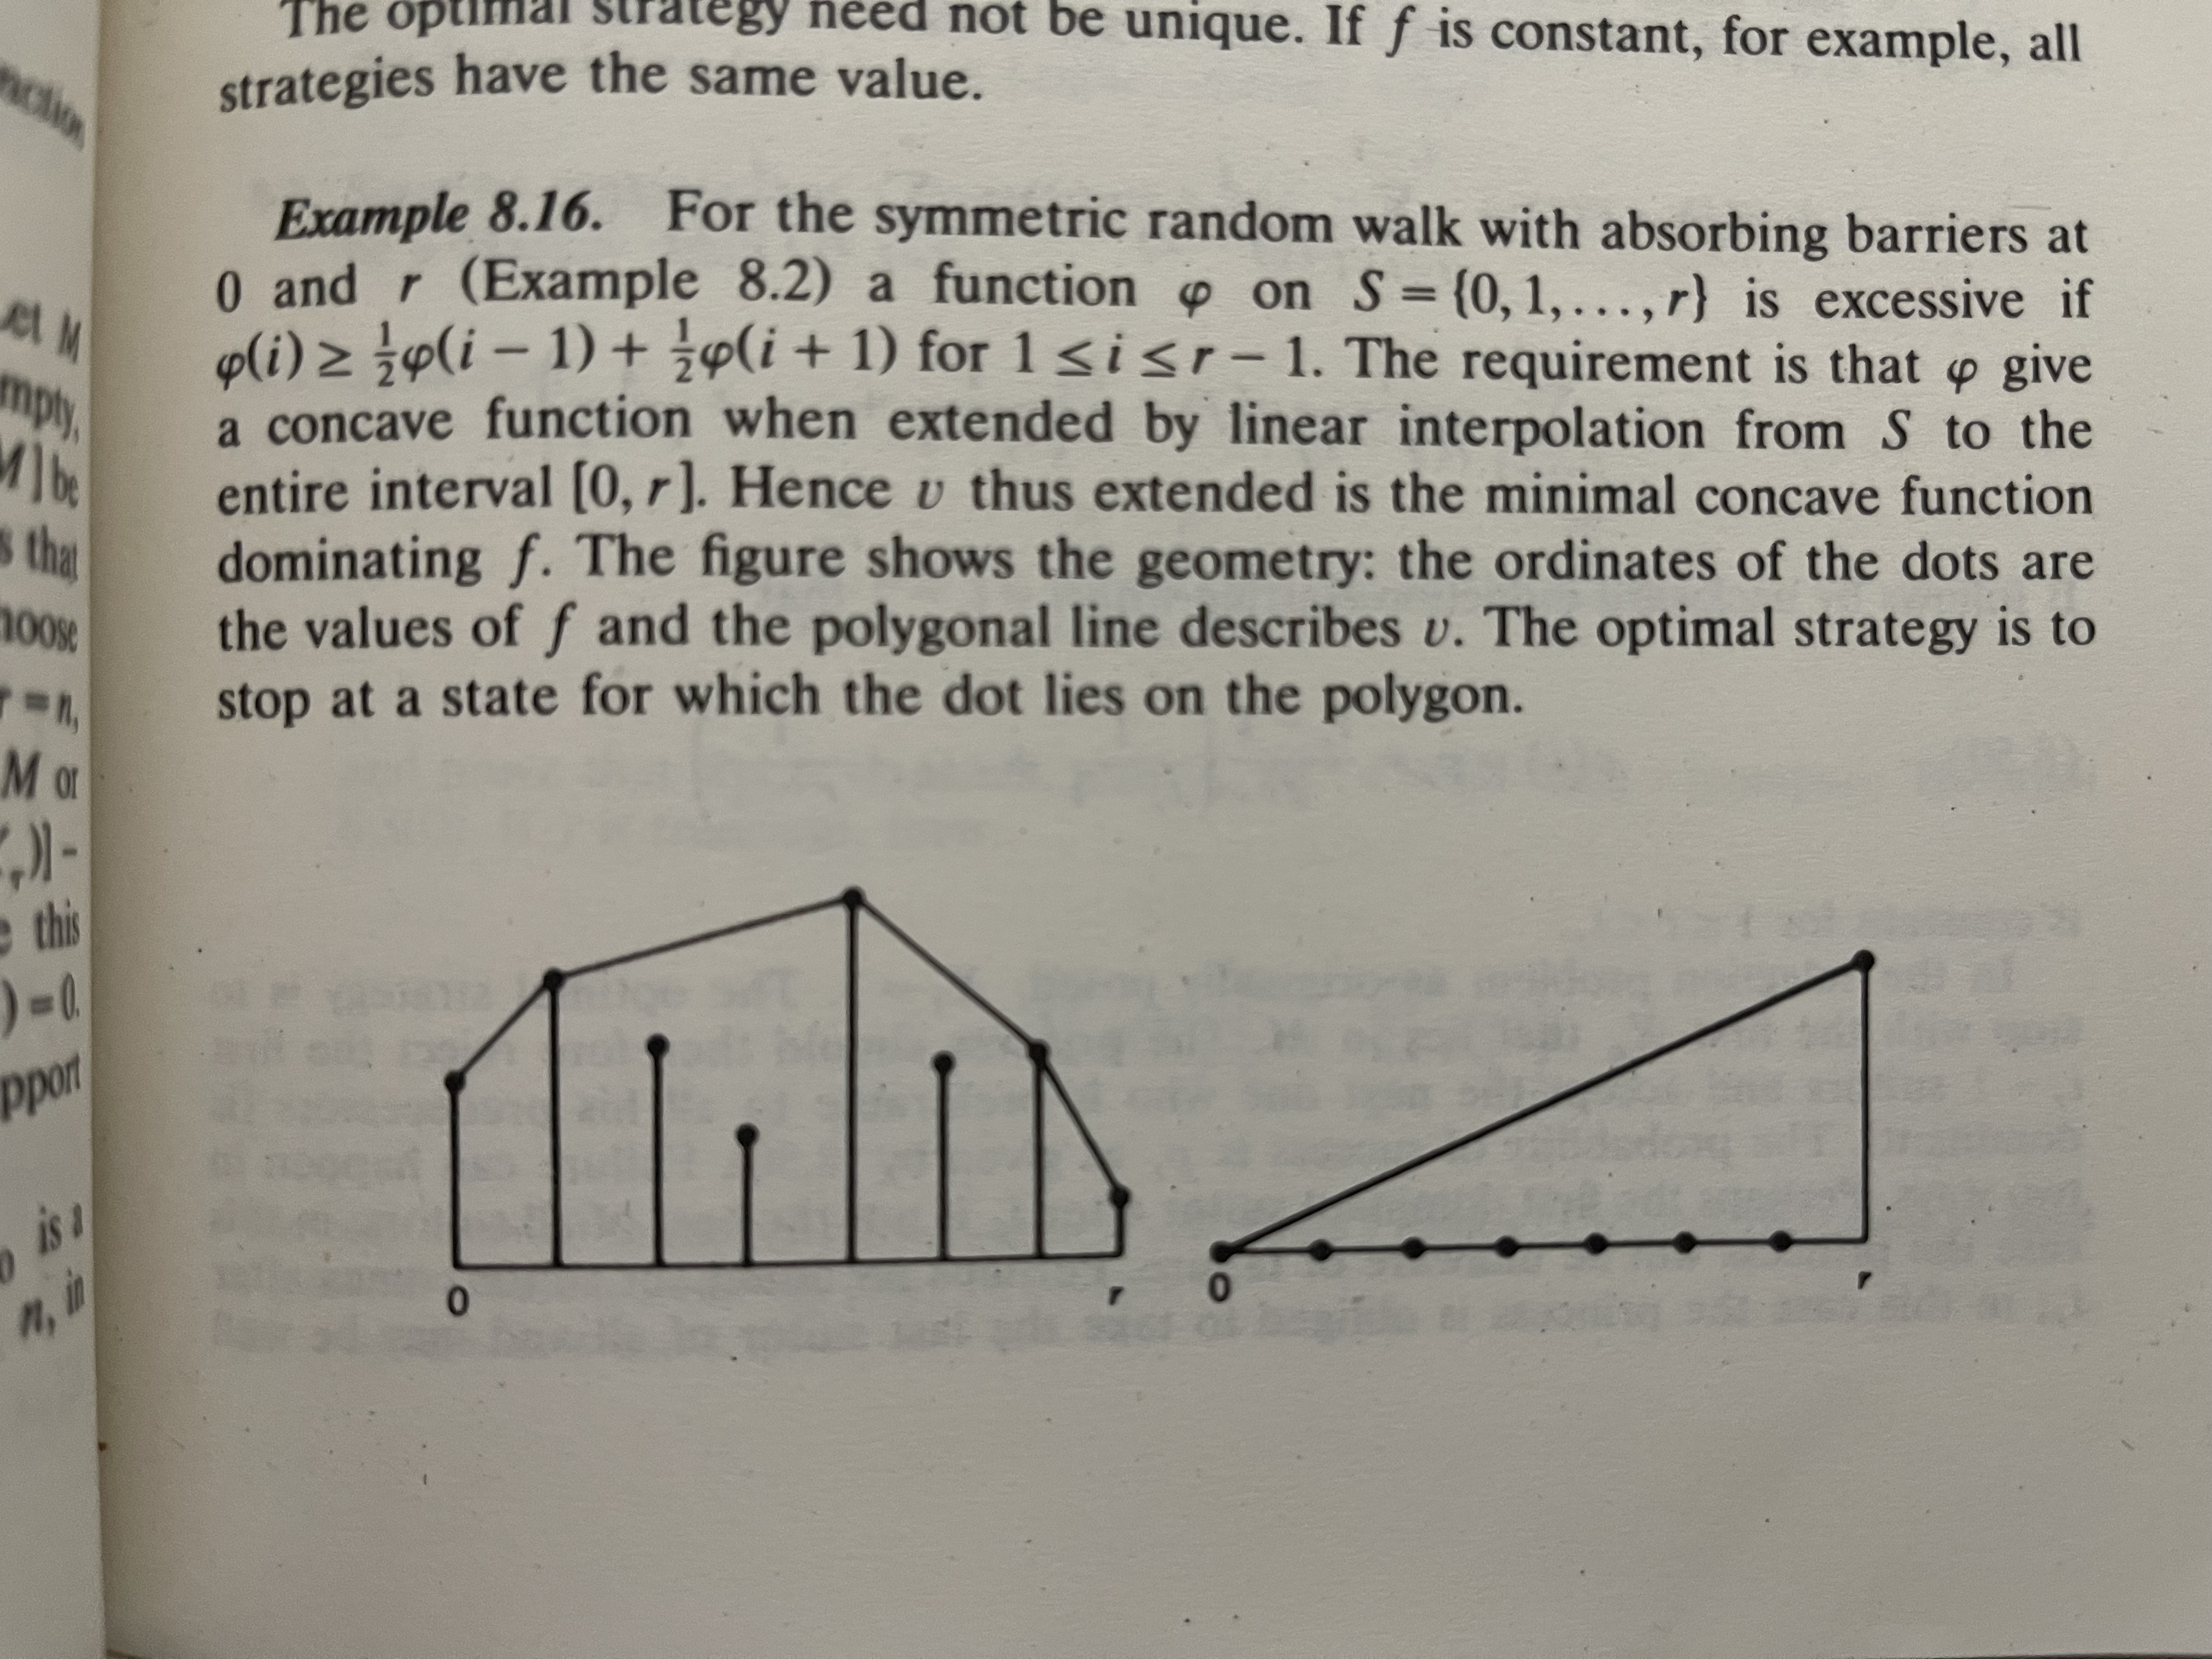
\includegraphics[width=0.8\textwidth]{excessive_concave.jpg}
	\caption{$v$ geometrically}
	\label{fig:excessive_concave_1}
\end{figure}
Note that to dominate $f$, the function $v$ has to be above the points that meet the dots in the picture. However, we also require $v$ to be concave. The minimal ``concavity" is a straight line - as this gives us equality on the concave condition. And so, for the symmetric random walk with absorbing barriers - the set of $M$ are the points that are on the convex hull (smallest polygon enclosing all points, with no inward curves. The bottom line and left and right line are included).
\\\\
I like this, because it ties a theoretical result to something that I think could be concluded intuitively. Note that in the left example, you would never stop at the inner points, as you will (with probability 1) go to a higher point. However, you do stop at the left and right line, because there is a high probability (1/2) that you will have to stop at a lower value.


\section{Section 9 - Large Deviations and The Iterated Logarithm}
\subsection{Notes} Note, I am skipping, as this is an optional chapter, and I am eager to continue on to general random variables and measure.


\section{Section 10 - General Measures}
\subsection{Notes}
\subsubsection{Classes of Sets} We want to find a analogues to the Borel sets for the entire real line, and $k$ dimensional Euclidean space. 

\paragraph{Example 10.1 - $k$ dimensional Borel Sets} Let $x = (x_1, \cdots ,x_k)$ be the generic point of Euclidean $k$ space $\R^k$. The bounded rectangles:
$$
	\left[x = (x_1, \cdots, x_k) : a_i < x_i \leq b_i, i = 1, \cdots, k\right]
$$
Will play in $\R^k$ the role intervals $(a,b]$ played in $(0,1]$. Let $\rcal^k$ be the $\sigma$ field generated by these rectangles. This is the analogue of the class $\bcal$ of Borel sets in $(0,1]$. The elements of $\rcal^k$ are the $k$-dimensional borel sets. For $k=1$, they are also called the linear Borel sets.
\\\\
Note that $\rcal^k$ contains the open sets. Each point in an open set contains an open rational rectangle - the countable union of these rectangles forms the open set, and so the open set is in the sigma field, being a countable union of sets in the field. As complements, the closed sets are also within $\rcal^k$. We can also find that $\rcal^k$ is generated by the open or closed sets (as intersections of open sets form the rectangles above). This also implies the rational rectangles generate $\rcal^k$. 
\\\\
Now, note the following. We have the sigma field $\rcal^1$, on the line $\R^1$, is by definition generated by the finite intervals. The field $\bcal$ in $(0,1]$ is generated by the subintervals of $(0,1]$. Note, $\R$ vs. $(0,1]$. The question is - are the elements of $\bcal$ the elements of $\rcal$ that happen to lie inside $(0,1]$? The short answer is yes - via the following theorem. We first note the definition: if $\acal$ is a class of sets in a space $\Omega$ and $\Omega_0$ is a subset of $\Omega$, let $\acal \cap \Omega_0 = \left[A \cap \Omega_0 : A \in \acal\right]$. We find:

\paragraph{Theorem 10.1}
\begin{enumerate}
	\item If $\fcal$ is a $\sigma$ field in $\Omega$, then $\fcal \cap \Omega_0$ is a $\sigma$ field in $\Omega_0$.
	\item If $\acal$ generates the $\sigma$ field $\fcal$ in $\Omega$, then $\acal \cap \Omega_0$ generates the $\sigma$ field $\fcal \cap \Omega_0$ in $\Omega_0: \sigma(\acal \cap \Omega_0) = \sigma(\acal) \cap \Omega_0$.
\end{enumerate}
\textbf{Proof:} The first proof is literally just your standard sigma field proof. Prove $\fcal \cap \Omega_0$ has $\Omega_0$, sets in it have their complements using $\fcal$, and countable unions of sets in it are in it as well, again using $\fcal$.
\\\\
Now, we get to the second part. Define $\fcal_0$ as $\sigma(\acal \cap \Omega_0)$, the generated $\sigma$ field \textit{in $\Omega_0$}. We must have that $\acal \cap \Omega_0 \subset \fcal \cap \Omega_0$, as every set in $\acal$ is in $\fcal$. As $\fcal$ is a $\sigma$ field, then $\fcal \cap \Omega_0$ is a $\sigma$ field by part 1, and so, by definition of the generated $\sigma$ field, we must have:
$$
	\fcal_0 \subseteq \fcal \cap \Omega_0 \text{ or, written another way }
	\sigma(\acal \cap \Omega_0) \subseteq \sigma(\acal) \cap \Omega_0
$$
We now want to prove the other direction, $\fcal \cap \Omega_0 \subseteq \fcal_0$. This will follow if it is shown $A \in \fcal$ implies $A \cap \Omega_0 \in \fcal_0$. Why? We want to show that for all $A \cap \Omega_0 \in \sigma(\acal) \cap \Omega_0$, we have that $A \cap \Omega_0 \in \sigma(\acal \cap \Omega_0) = \fcal_0$. Well, the $A \in \fcal$ by definition, so we are just kind of rewriting the statement. I think, we want to rewrite it in terms of just sigma fields in $\Omega$. We have $A \cap \Omega_0 \in \fcal_0$ if $A \in \gcal = \left[A \subset \Omega: A \cap \Omega_0 \in \fcal_0\right]$. So, we have:
$$
	\fcal \cap \Omega_0 \subseteq \fcal_0
$$
Is equivalent to us proving:
$$
	\fcal \subseteq \gcal
$$
So, we try and prove this. $A \in \acal$ implies $A \cap \Omega_0$ is in $\acal \cap \Omega_0 \in \fcal_0$, by definition. Thus, it follows $\acal \subset \gcal$. So, if we prove that $\gcal$ is a $\sigma$ field, we would have $\fcal = \sigma(\acal) \subseteq \gcal$. Note that $\Omega \in \gcal$, as $\Omega \cap \Omega_0 = \Omega_0 \in \fcal_0$. If $A \in \gcal$, then $(\Omega - A) \cap \Omega_0 = \Omega_0 - (A \cap \Omega_0) \in \fcal$, straight forward enough. Finally, if $A_n \in \gcal$ for all $n$, then $(\cup_n A_n) \cap \Omega_0 = \cup_n (A_n \cap \Omega_0) \in \fcal_0$.
\\\\
So, $\gcal$ is a $\sigma$ field, $\fcal \subseteq \gcal$, and we have thus proved:
$$
	\fcal_0 \supseteq \fcal \cap \Omega_0 \text{ or, written another way }
	\sigma(\acal \cap \Omega_0) \supseteq \sigma(\acal) \cap \Omega_0
$$
And thus, we have equality, and have proven the second statement. qed.

\paragraph{The Borel Sets lie in the Linear Borel Sets} The borel sets $\bcal$ refer to the sets in $(0,1]$. The linear borel sets refer to the sets in $\R^1$. If $\Omega = \R^1$, $\Omega_0 = (0,1]$, and $\acal$ is the set of half open intervals on the line, we have that $\rcal^1 = \sigma(\acal)$. By the above theorem, we thus have:
$$
	\sigma(\acal \cap (0,1]) = \sigma(\acal) \cap (0,1]
$$
Ie, $\rcal^1$, restricted to the unit interval (the RHS) is equal to the generated sigma algebra from the half open intervals in $(0,1]$ (the LHS), which is $\bcal$. Ie, we have:
$$
	\bcal = \rcal^1 \cap (0,1]
$$

\subsubsection{Measures}
\paragraph{Definition: Measure} A set function $\mu$ on a field $\fcal$ in $\Omega$ is called a \textit{measure} if it satisfies these conditions:
\begin{enumerate}
	\item $\mu(A) \in [0,\infty]$ for $A \in \fcal$
	\item $\mu(\emptyset) = 0$
	\item If $A_1, A_2, \cdots$ is a disjoint sequence of $\fcal$ sets and if $\bigcup_{k=1}^\infty A_k \in \fcal$, then:
	$$
		\mu\left(\bigcup_{k=1}^\infty A_k\right) = \sum_{k=1}^\infty \mu(A_k)
	$$
\end{enumerate}
I will note - the third condition doesn't require that all such unions are in $\fcal$, and $\fcal$ being a field doesn't guarantee it either. The measure $\mu$ is \textit{finite} or \textit{infinite} as $\mu(\Omega) < \infty$ or $\mu(\Omega) = \infty$. It is a probability measure if $\mu(\Omega) = 1$.

\paragraph{Definition: $\sigma$ finite} If $\Omega = A_1 \cup A_2 \cup \cdots$ for some finite or countable sequence of $\fcal$ sets satisfying $\mu(A_k) < \infty$, then $\mu$ is $\sigma$-finite. This notion will be significant later on. By our above definitions of finite/infinite measure, a finite measure is clearly $\sigma$ finite, and a $\sigma$ finite measure may be finite or infinite. If $\acal$ is a subclass of $\fcal$, and $\Omega = \cup_k A_k$ for some finite or infinite sequence of $\acal$ sets satisfying $\mu(A_k) < \infty$, then $\mu$ is \textit{$\sigma$ finite on $\acal$}.
\\\\
It is important to note that $\sigma$ finiteness is a joint property of the space $\Omega$, the measure $\mu$, and the class $\acal$.

\paragraph{Definition: Measure Space} If $\mu$ is a measure on a $\sigma$ field $\fcal$ in $\Omega$, the triple $(\Omega, \fcal, \mu)$ is a \textit{measure space} - note, not used if $\fcal$ is only a field. It is $\sigma$ finite, infinite, or finite based on whether $\mu$ has that property. If $\mu(A^c) = 0$ for an $\fcal$ set $A$, then $A$ is a \textit{support} of $\mu$, and $\mu$ is \textit{concentrated} on $A$. For a finite measure, $A$ is a support if and only if $\mu(A) = \mu(\Omega)$.

\paragraph{Example 10.2 - Discrete Space} A measure $\mu$ on $(\Omega, \fcal)$ (called a measurable space) is \textit{discrete} if there are finitely or countable many points $\omega_i$ in $\Omega$ and masses $m_i$ in $[0,\infty]$ such that $\mu(A) = \sum_{\omega_i \in A} m_i$ for $A \in \fcal$. 

\paragraph{Example 10.3 - The Counting Measure} Let $\fcal$ be the $\sigma$ field of all subsets of an arbitrary $\Omega$, and let $\mu(A)$ be the number of points in $A$, where $\mu(A) = \infty$ if $A$ is not finite. Then, $\mu$ is the \textit{counting measure}. It is finite if and only if $\Omega$ is finite, and is $\sigma$ finite if and only if $\Omega$ is countable.

\paragraph{Carry Over from Probability Measures to General Measures} A lot of the properties we derived for probability measures carry over to general measures. Note that:
\begin{enumerate}
	\item $\mu$ is monotone: examine $\mu(B) = \mu(A) + \mu(B - A)$
	\item We can only write $\mu(B - A) = \mu(B) - \mu(A)$ if $\mu(B) < \infty$
	\item We still have the inclusion-exclusion principle
	\item We still have the proof of finite subadditivity, as before:
	$$
		\mu\left(\bigcup_{k=1}^n A_k\right) \leq
		\sum_{k=1}^n \mu(A_k)
	$$
	The proof being just replace $A_k$ with $B_k$, which is disjoint from all the previous $A_k$. Note $\mu(B_k) \leq \mu(A_k)$.
\end{enumerate}

\paragraph{Theorem 10.2} Let $\mu$ be a measure on a field $\fcal$. We have:
\begin{enumerate}
	\item \textbf{Continuity From Below} If $A_n$ and $A$ lie in $\fcal$ and $A_n \uparrow A$, then:
	$$
		\mu(A_n) \uparrow \mu(A)
	$$
	
	\item \textbf{Continuity form Above} If $A_n$ and $A$ lie in $\fcal$ and $A_n \downarrow A$, and if $\mu(A_1) < \infty$ (or any $\mu(A_k) < \infty$) then:
	$$
		\mu(A_n) \downarrow \mu(A)
	$$
	
	\item \textbf{Countable Subadditivity} If $A_1, A_2, \cdots$, and $\bigcup_{k=1}^\infty A_k$ lies in $\fcal$, then:
	$$
		\mu\left(\bigcup_{k=1}^\infty A_k\right) \leq \sum_{k=1}^\infty \mu(A_k)
	$$
	
	\item If $\mu$ is $\sigma$ finite on $\fcal$, then $\fcal$ cannot contain an uncountable, disjoint collection of sets of positive $\mu$-measure.
\end{enumerate}
\textbf{Proof:} The proof for $1$ is the same as it is for probability measure: express $A$ as a disjoint union of $B_k$ (each $B_k$ represents the increment added to $A_k$ from $A_{k-1}$), and note limit sums are equal to $A_k$. The proof for $3$ is also the same as it is for probability measure: use part $1$ expressing the union as $\uparrow$, and then use the same reasoning as for finite additivity.
\\\\
The proof is essentially the same for $2$: if $\mu(A_1) < \infty$, subtraction is possible and $A_1 - A_n \uparrow A_1 - A$ implies that $\mu(A_1) - \mu(A_n) = \mu(A_1 - A_n) \uparrow \mu(A_1 - A) = \mu(A_1) - \mu(A)$, now just rearrange.
\\\\
So, the real meat comes in part 4. Let $\left[B_\theta: \theta \in \Theta\right]$ be a disjoint collection of $\fcal$ sets satisfying $\mu(B_\theta) > 0$. We will prove that $\Theta$ must be countable. Consider an $\fcal$ set $A$ for which $\mu(A) < \infty$. If $\theta_1, \cdots, \theta_n$ are distinct indices satisfying:
$$
	\mu\left(A \cap B_{\theta_i}\right) \geq \epsilon > 0
$$
Then we must have:
$$
	n\epsilon \leq \sum_{i=1}^n \mu(A \cap B_{\theta_i}) \leq \mu(A)
$$
And so:
$$
	n \leq \mu(A)/\epsilon
$$
Thus, we must have that the index set:
$$
	\left[\theta: \mu(A \cap B_{\theta}) > \epsilon\right]
$$
Is finite. If it wasn't - we could make a contradiction proving for some $B \subset A$, we have $\mu(B) > \mu(A)$. If we take a union over positive rational $\epsilon$, we must have:
$$
	\left[\theta: \mu(A \cap B_\theta) > 0\right]
$$
Is a countable index set. As $\mu$ is $\sigma$ finite, $\Omega = \cup_k A_k$ for $\mu(A_k) < \infty$, $A_k \in \fcal$. But then, define the index set:
$$
	\Theta_k = \left[\theta: \mu(A_k \cap B_\theta) > 0\right]
$$
$\Theta_k$ must be countable. As $\mu(B_\theta) > 0$, there must be a $k$ such that $\mu(A_k \cap B_\theta) > 0$ - if they all equaled zero, we would have a contradiction with countable subadditivity. Thus, each $B_\theta$ must appear in one of the $\Theta_k$ sets. And so:
$$
	\Theta = \bigcup_k \Theta_k
$$
And thus $\Theta$ is countable. qed.

\subsubsection{Uniqueness} 
According to Theorem 3.3, probability measures agreeing on a $\pi$ system $\pcal$ agree on $\sigma(\pcal)$ - this is by the $\pi$ $\lambda$ theorem. There is an extension in the general case

\paragraph{Theorem 10.3 - Uniqueness of General Measure Extension} Suppose that $\mu_1$ and $\mu_2$ are measures on $\sigma(\pcal)$, where $\pcal$ is a $\pi$ system, and suppose they are $\sigma$ finite on $\pcal$ (ie, countable $\pcal$ sets with non infinite measure union to $\Omega$). If $\mu_1$ and $\mu_2$ agree on $\pcal$, then they agree on $\sigma(\pcal)$.
\\\\
\textbf{Proof} Suppose that $B \in \pcal$ and $\mu_1(B) = \mu_2(B) < \infty$, and let $\lcal_B$ be the class of sets $A$ in $\sigma(\pcal)$ for which $\mu_1(B \cap A) = \mu_2(B \cap A)$. Then $\lcal_B$ is a $\lambda$ system (clearly contains $\omega$, complements by subtraction and $\mu(B) < \infty$, and countable disjoint unions via additivity of $\mu$) containing $\pcal$ ($\pi$ system contains intersections) and hence containing $\sigma(\pcal)$ via the $\pi-\lambda$ theorem.
\\\\
By $\sigma$-finiteness, there exists $\pcal$ sets $B_k$ satisfying $\Omega = \bigcup_k B_k$ and $\mu_1(B_k) = \mu_2(B_k) < \infty$. By inclusion-exclusion:
$$
	\mu_\alpha\left(\bigcup_{i=1}^n (B_i \cap A)\right) = \sum_{1 \leq i \leq n} \mu_\alpha(B_i \cap A) -
	\sum_{1 \leq i < j \leq n} \mu_\alpha(B_i \cap B_j \cap A) + \cdots
$$
For $\alpha = 1, 2$ and all $n$. Since $\pcal$ is a $\pi$ system, it contains all the intersections of $B_i$, and via the above argument, the terms on the RHS above are equal for $\mu_1$ and $\mu_2$. The LHS is thus equal for both as well. Now, we take $n \to \infty$, and use continuity from below, to find:
$$
	\mu_1(A) = \lim_{n \to \infty} \mu_1\left(\bigcup_{i=1}^n (B_i \cap A)\right) =
	\mu_2\left(\bigcup_{i=1}^n (B_i \cap A)\right) = \mu_2(A)
$$
For $A \in \sigma(\pcal)$. Thus, we have equality on $\sigma(\pcal)$. qed.

\paragraph{Theorem 10.4} Suppose $\mu_1$ and $\mu_2$ are finite measures on $\sigma(\pcal)$, where $\pcal$ is a $\pi$ system and $\Omega$ is a finite or countable union of sets in $\pcal$. If $\mu_1$ and $\mu_2$ agree on $\pcal$, then they agree on $\sigma(\pcal)$.
\\\\
\textbf{Proof} By hypothesis, $\Omega = \bigcup_k B_k$ for $\pcal$ sets $B_k$, and we of course have $\mu_\alpha(B_k) < \mu_\alpha(\Omega) < \infty$. So, $\mu_1$ and $\mu_2$ are $\sigma$ finite on $\pcal$, and Theorem 10.3 above applies. qed.

\subsection{Problems}
\subsubsection{10.1 Equivalent Measure Definition} Show that if conditions $(i)$ and $(iii)$ in the definition of measure hold, and if $\mu(A) < \infty$ for some $A \in \fcal$, then condition $(ii)$ holds.
\\\\
We note that by countable additivity:
$$
	\mu\left(A \cup \emptyset\right) = \mu(A) + \mu(\emptyset) \implies
	\mu(A) - \mu(A) = \mu(\emptyset) \implies \mu(\emptyset) = 0
$$
Note, we require $\mu(A) < \infty$, as otherwise subtraction is not defined.

\subsubsection{10.2 Finite vs. Countable Additivity on a Countable $\Omega$} On the $\sigma$ field of all subsets of $\Omega = \{1, 2, \cdots\}$ put $\mu(A) = \sum_{k \in A} 2^{-k}$ if $A$ is finite and $\mu(A) = \infty$ otherwise. Is $\mu$ finitely additive? Countably additive?
\\\\
I would first say that $\mu$ is finitely additive. If you have the finite disjoint union of finite sets - then we will just get out the sum. If you add a countable set in there - both sides will be infinite. Note, a finite amount of finite sets won't get to countable additivity.
\\\\
The issue comes with a countable amount of finite sets. Take $A_k = \{k\}$. We have:
$$
	\mu(\bigcup A_k) = \infty
$$
Clearly. However, we also have:
$$
	\sum_k \mu(A) = \sum_k 2^{-k} = 1
$$
So that is where countable additivity breaks down.

\subsubsection{10.3 Continuity From Above Extension}
\begin{enumerate}
	\item In connection with Theorem 10.2(ii), show that if $A_n \downarrow A$ and $\mu(A_k) < \infty$ for some $k$, then $\mu(A_n) \downarrow \mu(A)$. Note, I actually noted this in the theorem. You can make use of the first $\mu(A_k) < \infty$, instead of $A_1$.
	
	\item Find an example in which $A_n \downarrow A$, $\mu(A_n) = \infty$ for all $n$, and $A = \emptyset$.
	\\\\
	I think, we could take $\fcal = \rcal^1$, and I think its corresponding measure in the next section, $\lambda$. We have that $A_n = \bigcup_{k = n}^\infty (n, n+1]$ (note, I could write $(n, \infty)$, but I think this makes it clearer that it is within the first linear borel set). Clearly $A_n \downarrow A = \emptyset$. Take an $x \in \R$, clearly it doesn't belong to some $A_n$. We also have $\mu(A_n) = \infty$, again via additivity of the measure.
	\\\\
	Perhaps, that isn't the best example, as we haven't defined it yet. We could do the counting measure on $\Omega = \{1, 2, \cdots\}$ with $\fcal = 2^\Omega$. Same idea, $A_n = \{n, n + 1, \cdots\}$. 
\end{enumerate}

\subsubsection{10.4 Generalization of $\lim, \liminf, \limsup$ ordering} Recall Theorem 4.1 part 1: For each sequence of sets $A_n$:
$$
	P\left[\liminf_n A_n\right] \leq \liminf_n P(A_n) \leq \limsup_n P(A_n) \leq
	P\left[\limsup_n A_n\right]
$$
We want to generalize for arbitrary measures:
$$
	\mu\left[\liminf_n A_n\right] \leq \liminf_n \mu(A_n) \leq \limsup_n \mu(A_n) \leq
	\mu\left[\limsup_n A_n\right]
$$
Show that the left inequality always holds, and the right inequality holds if $\mu\left(\bigcup_{k \geq n} A_k\right) < \infty$ for some $n$.
\\\\
Note, these restrictions come from when we can conclude continuity from above/below. Let $B_n = \bigcap_{k \geq n} A_k$ and $C_n = \bigcup_{k \geq n} A_k$. Note that $B_n \uparrow \liminf_n A_n$. So, by Theorem 10.2, we have:
$$
	\mu\left[\liminf_n A_n\right] = \lim_n \mu(B_n) = \liminf_n \mu(B_n) \leq
	\liminf_n \mu(A_n)
$$
Note, the liminf always exists. We similarly note that $C_n \downarrow \limsup_n A_n$ - by the extension to Theorem 10.2 in the previous problem, if there is some $\mu(C_n) < \infty$, then we have:
$$
	\mu\left[\limsup_n A_n\right] = \lim_n \mu(C_n) = \limsup_n \mu(C_n) \geq \limsup_n \mu(A_n)
$$

\begin{comment}
	\subsection{10.5 Construct a Complete Measure Space} A measure space $(\Omega, \fcal, \mu)$ is \textit{complete} if $A \subset B$, $B \in \fcal$ and $\mu(B) = 0$ together imply $A \in \fcal$. Use the ideas of problem 3.10 to construct a complete measures space $(\Omega, \fcal^+, \mu^+)$ such that $\fcal \subset \fcal^+$ and $\mu$ and $\mu^+$ agree on $\fcal$.
	
	Note: I think this problem comes too early. First let us define a unique extension, so that we know if a complete space even exists
\end{comment}

\subsubsection{10.6 Characterizing $\sigma$ finiteness} The condition in Theorem 10.2(iv) essentially characterizes $\sigma$ finiteness.
\begin{enumerate}
	\item Suppose that $(\Omega, \fcal, \mu)$ has no ``infinite atoms" in the sense that for every $A \in \fcal$, if $\mu(A) = \infty$, then there is in $\fcal$ a $B$ such that $B \subset A$ and $0 < \mu(B) < \infty$. Show that if $\fcal$ does not contain an uncountable, disjoint collection of sets of positive measure, then $\mu$ is $\sigma$ finite (Use Zorn's lemma).
	\\\\
	Zorn's Lemma States: If $P$ is a partially ordered set (has an inequality, but not every element is comparable) such that every ordered chain has an upper bound in $P$ (ie, every chain of inequalities has an element greater than every element in the chain), then $P$ has at least one maximal element (an element such that no other element is greater than it).
	\\\\
	So now, we know that $\fcal$ does not contain an uncountable disjoint collection of sets of positive measure, and $\fcal$ does not have any infinite atoms.
	\\\\
	I think it can be done in the following way - iteratively. Assume $\mu$ is not $\sigma$ finite. Define $\fcal_1$ as the set of $A \in \fcal$ such that $\mu(A) < \infty$, or $A = \bigcup A_i$ where $\mu(A_i) < \infty$ and $A_i \cap A_j = \emptyset$. Note, $\fcal_1$ is partially ordered by $\subseteq$. Each chain of elements is bounded above - a countable chain is clear, but consider an uncountable one. Say we have an uncountable chain, with an uncountable amount of distinct sets. Then, this is a contradiction - because:
	$$
		A_1 \subset A_2 \implies A_2 - A_1 \in \Omega
	$$
	But then, we have an uncountable amount of disjoint sets in $\Omega$. So, this is a contradiction. So, our chains are countable, are all bounded - Zorn's lemma tells us there exists a maximal element $C_1 \in \fcal_1$.
	\\\\
	This is actually incorrect, I think. We are allowed to have uncountable, disjoint sets, if they have zero measure. We could have $\mu(A_1) = \mu(A_2)$, with $A_1 \subseteq A_2$.
	\\\\
	\textbf{Real Proof} First, we consider the case where $\fcal$ is countable. Take a union of every $\mu(A) < \infty$. Examine:
	$$
		\Omega - \bigcup A = C
	$$
	We want to show $C = \emptyset$. If that is not the case, note that $\mu(C) < \infty$ is a contradiction, as then $C$ would be included in the union. So, we must have $\mu(C) = \infty$. Note, we have assumed there are no infinite atoms, and so there must be some $B \subset C$ where $\mu(B) < \infty$. However, this leads to another contradiction, $B$ is then within our union, but $B$ is also outside of it. So, if $C \neq \emptyset$, we always have a contradiction, and we must thus have $\Omega$ is $\sigma$ finite (as the union above is uncountable).
	\\\\
	Now, we consider the case where $\fcal$ is uncountable. Let $\ical$ index every countable union of non-infinite measure sets. Ie, for $i \in \ical$, we have that:
	$$
		C_i = \bigcup_{j=1}^\infty C_{ij} \quad\text{ such that } \mu(C_{ij}) < \infty
	$$
	By contradiction, assume that $\Omega$ is not $\sigma$ finite. Then, for every $i \in \ical$, we must have:
	$$
		A_i = \Omega - C_i \quad\implies\quad A_i \neq \emptyset
	$$
	We note that $\mu(A_i) < \infty$ leads to a contradiction, as then $C_i \cup A_i$ is a countable union of non infinite measure sets that equals $\Omega$. So, we must have $\mu(A_i) = \infty$. As we have no infinite atoms, we must have a $B_i \subset A_i$ such that $0 < \mu(B_i) < \infty$.
	\\\\
	Use the axiom of choice, I guess, to select the $B_k$ that are disjoint from $B_i$. We note that there must be an uncountable amount of them. Assume that there is only a countable amount - note, we can easily create a countable amount of them. List them all out, from $B_1, B_2, \cdots$. As they are countable, we are able to list them in such a way. Now note:
	$$
		C_t = B_i \cup \bigcup_{k=1}^\infty B_k
	$$
	Forms a countable union in our index, which is why we set the above equal to $C_t$. This yields $B_t$, another positive measure set that is disjoint from the countable list we gave above, of every disjoint positive measure set from $B_i$. Thus, assuming that the set of $B_k$ that are disjoint from $B_i$ is countable is a contradiction, as any such countable set containing everything can yield another set that should be in there, but isn't.
	\\\\
	Thus, the $B_k$ that are disjoint from $B_i$ must be uncountable. Thus, assuming that $A_i$ is not empty for each countable union of non infinite measure sets leads to a contradiction that $\fcal$ contains an uncountable, disjoint collection of sets of positive measure. So, we must have for some $i$, $A_i = \emptyset$, and thus $\Omega$ is $\sigma$ finite. qed.
	
	\item Show by example that this is false without the condition that there are no infinite atoms.
	\\\\
	Maybe let $\fcal$ be the $\sigma$ algebra containing the two sets, the even integers and the odd integers, in $\Z$. Note, this $\fcal$ doesn't contain an uncountable disjoint collection of sets of positive measure. Note, however, $\fcal$ contains infinite atoms. $\mu$ is not $\sigma$ finite either, as we cannot express $\Omega$ as a countable union of finite measure sets.
\end{enumerate}

\section{Section 11 - Outer Measure}
\subsection{Notes}
\subsubsection{Outer Measure} 
\paragraph{Definition - Outer Measure} An \textit{outer measure} is a set function $\mu^*$ that is defined for all subsets of a space $\Omega$ and has these four properties:
\begin{enumerate}
	\item $\mu^*(A) \in [0,\infty]$ for every $A \subset \Omega$
	\item $\mu^*(\emptyset) = 0$
	\item $\mu^*$ is monotone; $A \subset B$ implies $\mu^*(A) \leq \mu^*(B)$
	\item $\mu^*$ is countable subadditive; $\mu^*\left(\bigcup_n A_n\right) \leq \sum_n \mu^*(A_n)$
\end{enumerate}
The set function $P^*$, defined by (3.1) is an example. This generalizes:

\paragraph{Example 11.1 - General Outer Measure of a Set Function} Let $\rho$ be a set function on a class $\acal$ in $\Omega$. Assume that $\emptyset \in \acal$ and $\rho(\emptyset) = 0$, and that $\rho(A) \in [0,\infty]$ for $A \in \acal$; $\rho$ and $\acal$ are otherwise arbitrary. Put:
$$
	\mu^*(A) = \inf \sum_n \rho(A_n)
$$
Where the infimum extends over all finite and countable coverings of $A$ by $\acal$ sets $A_n$. If no such covering exists - take $\mu^*(A) = \infty$, following the convention that the infimum over the empty set in $\infty$.
\\\\
We have that $\mu^*$ is an outer measure. It clearly satisfies $1, 2, 3$. We just go over $4$. If $\mu^*(A_n) = \infty$ for some $n$, then obviously the inequality will trivially hold. Assume that each $A_n$ is finite. Cover each $A_n$ by $\acal$ sets $B_{nk}$ satisfying:
$$
	\sum_k \rho(B_{nk}) < \mu^*(A_n) + \epsilon/2^n
$$
Then, we note that all of these covers together cover the union, and so:
$$
	\mu^*\left(\bigcup_n A_n\right) \leq \sum_{n,k} \rho(B_{nk}) < \sum_n \mu^*(A_n) + \epsilon
$$
Take $\epsilon$ to zero as normal. Thus, $\mu^*$ is an outer measure.

\paragraph{$\mu^*$ Measurable} Define $A$ to be $\mu^*$-measurable if:
$$
	\mu^*(A \cap E) + \mu^*(A^c \cap E) = \mu^*(E)
$$
For every $E$. This is the general version of (3.4) used in section 3. By subadditivity, it is equivalent to saying $A$ satisfies:
$$
	\mu^*(A \cap E) + \mu^*(A^c \cap E) \leq \mu^*(E)
$$
Denote $\mcal(\mu^*)$ as the class of $\mu^*$ measurable sets. The book now notes - we can replace $P^*$ with $\mu^*$, and $\mcal$ with $\mcal(\mu^*)$, symbol by symbol, and the proof still holds for lemmas 3.1, 3.2, 3.3. I will just list out their statements here:
\begin{enumerate}
	\item Lemma 3.1 - The class $\mcal(\mu^*)$ is a field. Yeah, it makes sense - $\mcal(\mu^*)$ is clearly closed under complements and similarly closed under intersections.
	
	\item Lemma 3.2 - If $A_1, A_2, \cdots$ is a finite or infinite sequence of disjoint $\mcal(\mu^*)$ sets, then for each $E \subset \Omega$:
	$$
		\mu^*\left(E \cap \left(\bigcup_k A_k\right)\right) = \sum_k \mu^*\left(E \cap A_k\right)
	$$
	Again, yeah, the lemma still makes sense.
	
	\item Lemma 3.3 - The class $\mcal(\mu^*)$ is a $\sigma$ field, and $\mu^*$ restricted to $\mcal$ is countably additive. Yeah, this still makes sense.
\end{enumerate}
If $\mu^*$ is countably additive, and also satisfies the properties 1, 2, 3, 4, we can also conclude it is a measure. So, we have the following theorem:

\paragraph{Theorem 11.1 - Induced Measure} If $\mu^*$ is an outer measure, then $\mcal(\mu^*)$ is a $\sigma$ field, and $\mu^*$ restricted to $\mcal(\mu^*)$ is a measure.

\subsubsection{Extension}
\paragraph{Theorem 11.2 - Extension of a Measure} A measure on a field has an extension to the generated $\sigma$ field.
\textbf{Proof:} Note, we don't need to prove this, as the result will actually follow from a strong form of the proof in Theorem 11.3. qed. Also note - if the original measure on the field is $\sigma$ finite, Theorem 10.3 implies that the extension is unique. Recall, Theorem 10.3 says that if there are two measure on a generated sigma field, and the generator is a $\pi$ system, and the measures agree on the $\pi$ system and are $\sigma$ finite (note, one is $\sigma$ finite implies the other is), then they agree on the entire generated sigma field.

\paragraph{Definition - Semi-Ring} A class of sets $\acal$ is a \textit{semiring} if:
\begin{enumerate}
	\item $\emptyset \in \acal$
	\item $A, B \in \acal$ implies $A \cap B \in \acal$
	\item $A, B \in \acal$ and $A \subset B$ implies there exists disjoint $C_1, \cdots, C_n \in \acal$ such that:
	$$
		B - A = \bigcup_{k=1}^n C_k
	$$
\end{enumerate}
Some simple examples - the class of finite intervals in $\Omega = \R^1$. Clearly the intersection of two such finite intervals is a finite interval. The set minus is also at most a pair of disjoint intervals. Also, the class of subintervals of $\Omega = (0,1]$ is a semiring as well, with the same reasoning. Every field is a semiring as well, as:
$$
	B - A = B \cap A^c \in \fcal
$$

\paragraph{Theorem 11.3 Measure Semi-Ring Extension} Suppose that $\mu$ is a set function on a semiring of $\acal$. Suppose that $\mu$ has values in $[0,\infty]$, $\mu(\emptyset) = 0$, and $\mu$ is finitely additive and countably subadditive. Then $\mu$ extends to a measure on $\sigma(\acal)$.
\\\\
First note - this contains Theorem 11.2. A field is clearly a semiring. A measure also satisfies all the given properties, definitionally, on $\acal$.
\\\\
\textbf{Proof:} Let $A, B$, $C_k$ be as in condition 3 of the semiring. By finite additivity:
$$
	\mu(B) = \mu(A) + \sum_{k=1}^n \mu(C_k) \geq \mu(A)
$$
Thus, our set function $\mu$ is monotone on $\acal$. Take our outer measure $\mu^*$ - recall, defined as:
$$
	\mu^*(A) = \inf \sum_n \mu(A_n)
$$
Where the infimum extends over coverings of $A$ by $\acal$ sets, and an empty infimum yields infinity. We first want to show that $\acal \subset \mcal(\mu^*)$. Then, if we show $\mu^*$ and $\mu$ agree on $\acal$, we can say that $\mu^*$ is our extension - Theorem 11.1 tells us that $\mu^*$ is a measure on $\mcal(\mu^*)$, and it would continue to be one when restricted to $\sigma(\acal)$.
\\\\
Take $A \in \acal$. If $\mu^*(E) = \infty$, then our condition for being in $\mcal(\mu^*)$:
$$
	\mu^*(A \cap E) + \mu^*(A^c \cap E) \leq \mu^*(E)
$$
holds trivially. So, assume $\mu^*(E) < \infty$. For an $\epsilon > 0$, use the definition of infimum to find $A_n$ such that:
$$
	\sum_n \mu(A_n) < \mu^*(E) + \epsilon
$$
As $A$ is a semiring, $B_n = A \cap A_n$ is in $\acal$, and $A^c \cap A_n = A_n - B_n$ has the form:
$$
	\bigcup_{k=1}^{m_n} C_{nk}
$$
Note that:
$$
	A_n = A \cap A_n \bigcup A^c \cap A_n = B_n \cup \bigcup_{k=1}^{m_n} C_{nk}
$$
Which is a disjoint union. Note that:
$$
	A \cap E \subset A \cap \bigcup_n A_n = \bigcup_n B_n
$$
Finally, note that:
$$
	A^c \cap E \subset A^c \cap \bigcup_n A_n =
	\bigcup_n A_n - B_n =
	\bigcup_n \bigcup_{k=1}^{m_n} C_{nk}
$$
We now conclude:
$$
	\mu^*(A \cap E) + \mu^*(A^c \cap E) \leq
	\sum_n \mu(B_n) + \sum_n \sum_{k=1}^{m_n} \mu(C_{nk}) =
	\sum_n \mu(A_n) < \mu^*(E) + \epsilon
$$
The first step is the definition of the outer measure - we take the infimum of covering sums, and as the $B_n$ and $C_{nk}$ are covering, we get less than the corresponding sums. The next equality is via finite additivity on $\acal$, and the $B_n$ and $C_{nk}$ being disjoint. Take $\epsilon \to 0$, and yes, we can conclude that $\acal \subset \mcal(\mu^*)$.
\\\\
Onto the next step. We want to show that $\mu^*$ and $\mu$ agree on $\acal$. If $A \subset \bigcup_n A_n$ for $\acal$ sets $A$ and $A_n$, then by countable subadditivity and monotonicity, we have:
$$
	\mu(A) \leq \sum_n \mu(A \cap A_n) \leq \sum_n \mu(A_n)
$$
Thus, $A \in \acal$ implies $\mu(A) \leq \mu^*(A)$. We note that $\mu^*(A) \leq \mu(A)$, just by the definition of the infimum, and so we can easily conclude that:
$$
	\mu(A) = \mu^*(A)
$$
And so now, we wrap up. We have:
$$
	\acal \subseteq \mcal(\mu^*) \implies
	\sigma(\acal) \subseteq \mcal(\mu^*)
$$
And $\mu^*$ restricted to $\sigma(\acal)$ is a measure. As $\mu^*$ agrees with $\mu$ on $\acal$, $\mu^*$ is a measure that is an extension of $\mu$ on $\sigma(\acal)$. qed.

\paragraph{Example 11.2 - Second Example of the Lebesgue Measure on the Unit Interval} Note that the subintervals of $\Omega = (0,1]$ is a \textit{semiring}. This is distinct from the disjoint finite unit of intervals, which is a field. For $\mu$ take length $\lambda(a,b] = b - a$. By Theorem 1.3, we already have that $\lambda$ is finitely additive and countably subadditive. By theorem 11.3, $\lambda$ extends to a measure on the class $\sigma(\acal) = \bcal$ of Borel sets in $(0,1]$. 

\paragraph{Example 11.3 - The Lebesgue Measure on the Real Line} Take $\acal$ as the semi ring of finite intervals on the real line $\R$, and $\lambda_1(a,b] = b - a$. We have that $\lambda_1$ is finitely additive and countably subadditive on $\acal$ (note Theorem 1.3 doesn't need to be restricted to $(0,1]$). Thus, $\lambda_1$ extends to the $\sigma$ field $\rcal^1$ of linear Borel sets, which is generated by $\acal$ definitionally. This defines the Lebesgue measure $\lambda_1$ over the whole real line.

\paragraph{The Lebesgue Measure on the Borel Set and the first Linear Borel Set Coincide} Recall, from Theorem 10.1, we have that a subset of $(0,1]$ lies in $\bcal$ iff it lies in $\rcal^1$ as well. We have that $\lambda_1(A) = \lambda(A)$, for $A$ subinterval of $(0,1]$ - just the length. It follows by uniqueness of extension that $\lambda_1(A) = \lambda(A)$ for all $A \in \bcal$. So, we don't need the $1$ subscript - just call is $\lambda$ as well.

\subsubsection{An Approximation Theorem}
By Theorem 10.3, we have that if two measures are sigma finite on a $\pi$ system $\pcal$, agree on $\pcal$, and are measures on $\sigma(\pcal)$, they also agree on $\sigma(\pcal)$. In this way, if $\acal$ is a semiring which is $\sigma$ finite, a measure on $\sigma(\acal)$ is thus determined by its values on $\acal$. We can thus approximate the measure of a $\sigma(\acal)$ set by measures of $\acal$ sets.

\paragraph{Lemma 11.1 - Semi Ring Intersection Equality} If $A, A_1, \cdots, A_n$ are sets in a semiring $\acal$, then there are disjoint $\acal$ sets $C_1, \cdots, C_m$ such that:
$$
	A \cap A_1^c \cap \cdots \cap A_n^c = C_1 \cup \cdots \cup C_m
$$
\textbf{Proof:} The case $n = 1$ follows from the definition of the semiring applied to $A \cap A_1^c = A - (A \cap A_1) = C_1 \cup \cdots \cup C_m$. Use induction. If the result holds for $n$, then:
$$
	A \cap A_1^c \cap \cdots \cap A_{n+1}^c = 
	\bigcup_{j=1}^m (C_j \cap A_{n+1}^c)
$$
And apply the case $n = 1$ to each set in the union.

\paragraph{Theorem 11.4 - Approximating the Measure With Semiring Values} Suppose that $\acal$ is a semiring, $\mu$ is a measure on $\fcal = \sigma(\acal)$, and $\mu$ is $\sigma$ finite on $\acal$.
\begin{enumerate}
	\item If $B \in \fcal$ and $\epsilon > 0$, there exists a finite or infinite disjoint sequence $A_1, A_2, \cdots$ of $\acal$ sets such that $B \subset \bigcup_k A_k$ and:
	$$
		\mu\left(\bigcup_k A_k - B\right) < \epsilon
	$$
	
	\item If $B \in \fcal$ and $\epsilon > 0$, and if $\mu(B) < \infty$, then there exists a finite disjoint sequence $A_1, \cdots, A_n$ of $\acal$ sets such that:
	$$
		\mu\left(B \triangle \bigcup_{k=1}^n A_k\right) < \epsilon
	$$
\end{enumerate}
\textbf{Proof:} Recall the proof of Theorem 11.3. If $\mu^*$ is the outer measure, we have $\fcal \subset \mcal(\mu^*)$. We also have that $\mu^*$ agrees with $\mu$ on $\acal$ (Theorem 11.3) and by uniqueness of extension agrees with $\mu$ on $\fcal$ ($\mu^*$ restricted to $\fcal$ is a measure).
\\\\
Take our $B \in \fcal$, and suppose $\mu(B) = \mu^*(B) < \infty$. There exist $\acal$ sets $A_k$ such that:
$$
	B \subseteq \bigcup_k A_k \quad\quad\quad
	\mu\left(\bigcup_k A_k\right) \leq \sum_k \mu(A_k) < \mu(B) + \epsilon
$$
By subadditivity, and definition of the outer measure. Thus, we have:
$$
	\mu\left(\bigcup_k A_k - B\right) < \epsilon
$$
To make the $A_k$ disjoint, replace $A_k$ with:
$$
	A_k \cap A_1^c \cap \cdots \cap A_{k-1}^c = C_{k1} \cup \cdots \cup C_{km_k}
$$
The equality follows by Lemma 11.1. So, we have prove 11.4.1 in the finite case. Now assume $\mu(B) = \mu^*(B) = \infty$. By $\sigma$-finiteness, there exists $\acal$ sets $C_m$ such that $\Omega = \bigcup_m C_m$ and $\mu(C_m) < \infty$. Note that $B \cap C_m \in \acal$ by semi ring closed under finite intersection, and $\mu(B \cap C_m) < \infty$. By the above finite case, there exists $A_{mk} \in \acal$ such that:
$$
	\mu\left(\bigcup_k A_{mk} - (B \cap C_m)\right) < \epsilon/2^m
$$
The sets $A_{mk}$, taken together, provide a countable sequence $A_1, A_2, \cdots$ of $\acal$ sets satisfying $\bcal \subset \bigcup_k A_k$ and:
$$
	\mu\left(\bigcup_k A_k - B\right) < \epsilon
$$
We can make the $A_k$ disjoint as before. This thus completely proves 11.4.1.
\\\\
Now, we go onto 11.4.2. Consider the $A_k$ of part 1 for $B$ with finite measure. For $A = \bigcup_k A_k$, we have $\mu(A) < \mu(B) + \epsilon$, and so $A$ has finite measure, and we can apply continuity from above to see (note, continuity from above on the sets $A - \bigcup_{k \leq 1} A_k, A - \bigcup_{k \leq 2} A_k, \cdots$) there is a finite $n$ such that:
$$
	\mu(A - \bigcup_{k \leq n} A_k) < \epsilon
$$
But then:
$$
	\mu\left(B \triangle \bigcup_{k \leq n} A_k\right) =
	\mu\left(\bigcup_{k \leq n} A_k - B\right) + \mu\left(B - \bigcup_{k \leq n} A_k\right)
$$
By finite additivity. By monotonicity:
$$
	\leq
	\mu\left(A - B\right) + \mu\left(A - \bigcup_{k \leq n} A_k\right) = 2\epsilon
$$
And thus, we have proved part 2 as well. qed.
\\\\
Just an interesting consequence. For any linear Borel Set $B$ of finite lebesgue measure, there is a disjoint finite collection of finite intervals $A_1, \cdots, A_n$ such that:
$$
	\lambda\left(B \triangle \bigcup_{k=1}^n A_k\right) < \epsilon
$$

\paragraph{Corollary 11.4.1 Approximation on Finite Measures} If $\mu$ is a finite measure on a $\sigma$ field $\fcal$ generated by a field $\fcal_0$, then for each $\fcal$ set $A$ and each positive $\epsilon$ there is an $\fcal_0$ set $B$ such that $\mu(A \triangle B) < \epsilon$.
\\\\
\textbf{Proof:} An immediate consequence of the above. For every $A \in \fcal$, we have $\mu(A) < \infty$, so there are $A_n$ $\fcal_0$ sets whose finite union symmetric difference with $A$ is less than $\epsilon$. However, $\fcal_0$ is a field, and so their finite union makes the $B$ in the statement.
\\\\
However, there is a simpler proof. Let $\gcal$ be the sets $A$ with the above property, note closed under complements (as $A^c \triangle B^c = A \triangle B$), closed under countable unions, and so $\gcal$ is a $\sigma$ field.

\paragraph{Corollary 11.4.2 Monotonicty Extends to $\sigma$ field} Suppose that $\acal$ is a semiring, $\Omega$ is a countable union of $\acal$ sets, and $\mu_1, \mu_2$ are measures on $\fcal = \sigma(\acal)$. If $\mu_1(A) \leq \mu_2(A) < \infty$ for $A \in \acal$, then $\mu_1(B) \leq \mu_2(B)$ for $B \in \fcal$.
\\\\
\textbf{Proof:} As $\mu_2$ is $\sigma$ finite on $\acal$ (as $\acal$ sets union to $\Omega$, and all $\acal$ sets have finite measure), Theorem 11.4 applies. Note the statement is trivial if $\mu_2(B) = \infty$. If $\mu_2(B) < \infty$, choose disjoint $\acal$ sets $A_k$ such that $B \subset \bigcup_k A_k$ and:
$$
	\sum_k \mu_2(A_k) < \mu_2(B) + \epsilon
$$
Then, note:
$$
	\mu_1(B) \leq \sum_k \mu_1(A_k) \leq \sum_k \mu_2(A_k) < \mu_2(B) + \epsilon
$$
Take $\epsilon$ to zero. qed.

\paragraph{Lemma 11.2 Monotonicity of Set Functions on a Semi-ring} Suppose that $\mu$ is a nonnegative and finitely additive set function on a semiring $\acal$, and let $A, A_1, \cdots, A_n$ be sets in $\acal$. 
\begin{enumerate}
	\item If $\bigcup_{i=1}^n A_i \subset A$ and the $A_i$ are disjoint, then $\sum_{i=1}^n \mu(A_i) \leq \mu(A)$
	\item If $A \subset \cup_{i=1}^n A_i$, then $\mu(A) \leq \sum_{i=1}^n \mu(A_i)$
\end{enumerate}
\textbf{Proof} For part 1 - make use of lemma 1 and choose disjoint $\acal$ sets $C_j$ such that:
$$
	A - \bigcup_{i=1}^n A_i = \bigcup_{j=1}^m C_j
$$
As $\mu$ is finitely additive and nonnegative, it follows that:
$$
	\mu(A) = \sum_{i=1}^n \mu(A_i) + \sum_{j=1}^n \mu(C_j) \geq \sum_{i=1}^n \mu(A_i)
$$
For part 2 - take $B_1 = A \cap A_1$, and $B_i = A \cap A_i \cap A_1^c \cap \cdots \cap A_{i-1}^c$ for $i > 1$. By Lemma 1, each $B_i$ is a finite disjoint union of $\acal$ sets $C_{ij}$. Note:
$$
	A = \bigcup_i B_i = \bigcup_{ij} C_{ij} \quad\quad\quad
	\cup_j C_{ij} \subset A_i
$$
As the $B_i$ are disjoint, all the $C_{ij}$ are disjoint, and finite additivity and part 1 tells us that:
$$
	\mu(A) = \sum_{ij} \mu(C_{ij}) \leq \sum_i \mu(A_i)
$$

\subsection{Problems}
\subsubsection{11.1 Measure Extension to $\sigma$ field without Theorem 11.3} The proof of Theorem 3.1 (a probability measure on a field has a unique extension to the generated $\sigma$ field) applies if the probability measure is replaced by a finite measure - it really is just a matter of rescaling, and above we proved all the steps are essentially the same.
\\\\
Take as a starting point then the fact that a finite measure on a field extends uniquely to the generated $\sigma$ field. With the following steps, we can prove Theorem 11.2 - ie, removing the assumption of finiteness - without relying on Theorem 11.3.
\begin{enumerate}
	\item Let $\mu$ be a measure (not necessarily even $\sigma$-finite) on a field $\fcal_0$, and let $\fcal = \sigma(\fcal_0)$. If $A$ is a nonempty set in $\fcal_0$ and $\mu(A) < \infty$, restrict $\mu$ to a finite measure $\mu_A$ on the field $\fcal_0 \cap A$, and extend $\mu_A$ to a finite measure $\hat{\mu}_A$ on the $\sigma$ field $\fcal \cap A$ generated in $A$ by $\fcal_0 \cap A$.
	\\\\
	To be honest - I don't think there is a question here. We do have that $\fcal_0 \cap A$ is still a field. We note that $\mu_A$ is still a measure on that field. It is finite, as we have $A$ is our $\Omega$, and $\mu_A(A) = \mu(A) < \infty$. We thus have, by the starting point, that $\mu_A$ finite measure on the field $\fcal_0 \cap A$ extends uniquely to:
	$$
		\sigma(\fcal_0 \cap A)
	$$
	Then, make use of Theorem 10-1. We have that $\fcal_0$ generates $\fcal$ in $\Omega$, and so $\fcal_0 \cap A$ generates the restricted $\sigma$ field $\sigma(\fcal_0) \cap A = \fcal \cap A$:
	$$
		\sigma(\fcal_0 \cap A) = \fcal \cap A
	$$
	
	\item Suppose that $E \in \fcal$. If there exist disjoint $\fcal_0$ sets $A_n$ such that $E \subset \bigcup_n A_n$ and $\mu(A_n) < \infty$, put:
	$$
		\hat{\mu}(E) = \sum_n \hat{\mu}_{A_n}(E \cap A_n)
	$$
	And prove consistency. Otherwise put $\hat{\mu}(E) = \infty$.
	\\\\
	So, suppose that we have two satisfying sequences, $E \subset \bigcup_n A_n$ and $E \subset \bigcup_n B_n$. We want to prove that $\hat{\mu}(E)$ is the same for both. We note - how is:
	$$
		\hat{\mu}_{A_n}(E \cap A_n)
	$$
	Defined? Well - note that $E \cap A_n \in \fcal \cap A_n$, and that $\hat{\mu}_{A_n}$ is well defined for that set - as an extension.
	\\\\
	To be honest - I don't think this is well defined. What if we are double counting? Like I feel we should at least take an infimum of some kind. Ohh - we assume disjoint. Ok. This actually makes it easier - because I think we should consider for two such disjoint sequences $A_n$ and $B_m$:
	$$
		\hat{\mu}(E) = \sum_n\sum_m \hat{\mu}_{A_n \cap B_m}(E \cap A_n \cap B_m)
	$$
	We want to show that the above is equal to $\hat{\mu}(E)$ defined on $A_n$ and $B_m$, in which case we will have equality between the two definitions. Mainly, I want to show:
	$$
		\hat{\mu}_{A_n}(E \cap A_n) = \sum_m \hat{\mu}_{A_n \cap B_m}(E \cap A_n \cap B_m)
	$$
	Recall - $\hat{\mu}_{A_n}$ is a measure on $\fcal \cap A_n$. Note that as $B_m \in \fcal_0$, we must have that $E \cap B_m \cap A_n \in \fcal \cap A_n$. Note that we have the $B_m$ are disjoint, and:
	$$
		E \cap A_n = E \cap A_n \cap \bigcup_m B_m
	$$
	And so, via countable additivity of a measure, we have:
	$$
		\hat{\mu}_{A_n}(E \cap A_n) = \sum_m \hat{\mu}_{A_n}(E \cap A_n \cap B_m)
	$$
	So really, we have consistency will follow, if we can show:
	$$
		\hat{\mu}_{A_n}(E \cap A_n \cap B_m) = \hat{\mu}_{A_n \cap B_m}(E \cap A_n \cap B_m)
	$$
	First, examine the core definition:
	$$
		\hat{\mu}_{A_n \cap B_m}(E \cap A_n \cap B_m) =
		\inf \sum_k \mu_{A_n \cap B_m}(D_k) =
		\inf \sum_k \mu(D_k)
	$$
	Where $D_k \in \fcal_0 \cap A_n \cap B_m$, and $\bigcup_k D_k \supseteq E \cap A_n \cap B_m$. Note, we must have that:
	$$
		D_k = D_k' \cap A_n \cap B_m \quad\quad\quad D_k' \in \fcal_0
	$$
	Thus, we have that via $\fcal_0$ being a field, $D_k' \cap B_m \in \fcal_0$, and so $D_k \in \fcal_0 \cap A_n$. Thus, every covering of $E \cap A_n \cap B_m$ in $\fcal_0 \cap A_n \cap B_m$ corresponds to a covering of $E \cap A_n \cap B_m$ in $\fcal_0 \cap A_n$, and so we must have via an infimum over a larger set:
	$$
		\hat{\mu}_{A_n}(E \cap A_n \cap B_m) \leq \hat{\mu}_{A_n \cap B_m}(E \cap A_n \cap B_m)
	$$
	Now, we want to go in the opposite direction. Examine a $C_k$ such that:
	$$
		\sum_k \mu_{A_n}(C_k) < \hat{\mu}_{A_n}(E \cap A_n \cap B_m) + \epsilon
	$$
	This via the definition of the infimum. Note that $\bigcup_k C_k \cap B_m$ still covers $E \cap A_n \cap B_m$, and so:
	$$
		\hat{\mu}_{A_n \cap B_m}(E \cap A_n \cap B_m) \leq
		\sum_k \mu_{A_n \cap B_m}(C_k \cap B_m) =
		\sum_k \mu(C_k \cap B_m) \leq
		\sum_k \mu(C_k)
	$$
	$$
		= \sum_k \mu_{A_n}(C_k) < \hat{\mu}_{A_n}(E \cap A_n \cap B_m) + \epsilon
	$$
	Take $\epsilon$ to zero, and so we also have:
	$$
		\hat{\mu}_{A_n}(E \cap A_n \cap B_m) \geq \hat{\mu}_{A_n \cap B_m}(E \cap A_n \cap B_m)
	$$
	Note, what we have implicitly used is that for sets in $\fcal_0 \cap A_n$ and $\fcal_0 \cap A_n \cap B_m$, $\mu_{A_n}(U) = \mu(U)$ and $\mu_{A_n \cap B_m}(U) = \mu(U)$, as the measures are just restrictions to smaller fields - ie, the values don't change. So, in all, we have:
	$$
		\hat{\mu}_{A_n}(E \cap A_n \cap B_m) = \hat{\mu}_{A_n \cap B_m}(E \cap A_n \cap B_m) =
		\hat{\mu}_{B_m}(E \cap A_n \cap B_m)
	$$
	Via symmetry. And so, we can conclude that the definition of $\hat{\mu}(E)$ is consistent.
	
	\item Show that $\hat{\mu}$ is a measure on $\fcal$ and agrees with $\mu$ on $\fcal_0$.
	\\\\
	First, we show that it is a measure on $\fcal$. We need it to be countably additive, and to have the empty set be measure $0$. Well, lets start with something easy. We have:
	$$
		\hat{\mu}(\emptyset) = \hat{\mu}_{A_n}(\emptyset \cap A_n) = 0
	$$
	Now, countable additivity. We take disjoint $E_1, E_2, \cdots$. If any of the $\hat{\mu}(E_n) = \infty$, we have the statement is true, so assume all are finite. We examine:
	$$
		\hat{\mu}\left(\bigcup_n E_n\right)
	$$
	I think, for each $E_n$, we can take a sequence $A_{nk}$ that are disjoint, in $\fcal_0$, and cover $E_n$ - that is what we get via assuming finiteness. Note that these $A_{nk}$ are still countable, and can be listed like $A_1, A_2, \cdots$ (a countable amount of countable sets is still countable). They can be formed into a disjoint cover of $\bigcup_n E_n$. This is via taking:
	$$
		B_1 = A_1 \quad\quad\quad
		B_2 = A_2 \setminus A_1 \quad\quad\quad
		B_3 = A_3 \setminus (A_1 \cup A_2)
	$$
	And so on. So, we have that we can find a cover of disjoint $\acal_0$ sets that cover the disjoint union in the case that each $\hat{\mu}(E_n) < \infty$. Thus, by definition, we have:
	$$
		\hat{\mu}\left(\bigcup_n E_n\right) =
		\sum_t \hat{\mu}_{B_t}\left(\bigcup_n E_n \cap B_t\right) =
		\sum_t \sum_n \hat{\mu}_{B_t}\left(E_n \cap B_t\right)
	$$
	The first equality is definitional, and the last one makes use of the fact that $\hat{\mu}$ is a measure, and so countable additivity applies for disjoint sets. Now, note that the sequence $B_1, B_2, \cdots$ is a disjoint sequence of $\fcal_0$ sets that cover each $E_n$ - so, they can also be used to apply the definition of $\hat{\mu}$. We find:
	$$
		= \sum_n \sum_t \hat{\mu}_{B_t}\left(E_n \cap B_t\right)
		= \sum_n \hat{\mu}(E_n)
	$$
	Where in the first equality we just switched the order of the sum (nonnegative sum, fine to switch). And so, we do have countable additivity. So, in total: $\hat{\mu}$ is defined for each $E \in \fcal$, returns a number in $[0,\infty]$, is zero for the $\emptyset$, and is countably additive. So, it is a measure. Now, we just want to show that $\hat{\mu}$ agrees with $\mu$ on $\fcal_0$. Well, we have that $\hat{\mu}$ is consistent. Note for $E \in \fcal_0$, we have that $E$ itself is a disjoint sequence covering $E$. And so, we have:
	$$
		\hat{\mu}(E) = \hat{\mu}_E(E \cap E) = \mu(E)
	$$
	And so in conclusion: we have constructed an extension for $\mu$ on a field $\fcal_0$, even if the measure is not finite on $\fcal_0$.
	
\end{enumerate}

\subsubsection{11.2 Countable Subadditivity on Rings} Suppose that $\mu$ is a nonnegative and finitely additive set function on a semiring $\acal$.
\begin{enumerate}
	\item Use Lemmas 1 and 2, without reference to Theorem 11.3, to show that $\mu$ is countably subadditive if and only if it is countably additive.
	
	\item Find an example where $\mu$ is not countably subadditive.
\end{enumerate}
So, for the first part. We have an if and only if. First, assume that $\mu$ is countably additive on its semiring. Ie, if $A_1, A_2, \cdots$ are in $\acal$ and disjoint, and the union is in $\acal$ as well, we have:
$$
	\mu\left(\bigcup_n A_n\right) = \sum_n\mu\left(A_n\right)
$$
We want to show this proves countable subadditivity. Take $B_1, B_2, \cdots$ in $\acal$. Assume their union is within $\acal$ as well. We have by Lemma 1:
$$
	B_n \cap B_1^c \cap \cdots \cap B_{n-1}^c = C_{n1} \cup \cdots \cup C_{nm_n}
$$
These $C$ form a disjoint union, whose union is $B$, the union of the $B_i$, which is in $\acal$. Countable additivity gives us:
$$
	\mu\left(\bigcup_n B_n\right) =
	\mu\left(\bigcup_{n,i} C_{ni}\right) =
	\sum_{n,i} \mu(C_{ni})
$$
Via finite additivity, it is clear that:
$$
	\sum_{i=1}^{m_n} \mu(C_{ni}) \leq \mu(B_n)
$$
So, that gives us:
$$
	\mu\left(\bigcup_n B_n\right) \leq \sum_n \mu(B_i)
$$
So countable additivity implies countable subadditivity. Now, go the other direction. Assume we have countable subadditivity. Thus, to show equality, we really just need to show for disjoint $A_n$, we have:
$$
	\mu\left(\bigcup_n A_n\right) \geq \sum_n\mu\left(A_n\right)
$$
This can come pretty directly from Lemma 2. We have that $A = \bigcup_n A_n$. We have that $\bigcup_{n=1}^k A_n \subseteq A$ clearly, and so by lemma 2 part 1 (as the $A_n$ are disjoint), we have:
$$
	\sum_{n=1}^k\mu\left(A_n\right) \leq \mu\left(\bigcup_n A_n\right)
$$
Now, just take a limit of $k \to \infty$ (we can take a limit on the sum), which will allow us to conclude countable additivity:
$$
	\mu\left(\bigcup_n A_n\right) = \sum_n\mu\left(A_n\right)
$$
qed. We now go to the second part - find an example of a semiring $\acal$ where $\mu$ is not countably subadditive. One simple semiring is the half open finite intervals on the real line $\R^1$. The intersection of two intervals is clearly a finite interval, and the set minus of finite intervals is a union of disjoint intervals. We are looking for a nonnegative, finitely additive, but not countably subadditive set function on this $\acal$.
\\\\
I will actually try a different ring - inspired by question 10.2. Let $\acal$ consist of subsets of $\Omega = \{1, 2, \cdots\}$, being intervals with no jumps - ie, we can not have something like $\{x, x + 2\}$ - if $x, y \in I$, then every integer between $x$ and $y$ must also be in the interval. We clearly contain intersections (as if $x,y$ are in both $I_1$, and $I_2$, each number between them is in the intersection) and setminuses are disjoint unions of sets in $\acal$.
\\\\
We let $\mu(I) = \sum_{k \in I} 2^{-k}$ if $I$ is finite and $\mu(I) = \infty$ if it contains a non finite amount of elements. It is clear that $\mu$ is finitely additive and nonnegative, similar to what was proved in 10.2. However, $\mu$ is not countably additive. Take sets $I_n = \{n\}$. There disjoint union is within $\acal$, but the disjoint sum is $1$, whereas the set function on the union is infinity.
\\\\
Now, we note by the above theorem - this implies that $\mu$ is also not countably subadditive. This can be the seen with the same example of $I_n = \{n\}$, as we have:
$$
	\infty = \mu(\cup_n I_n) \geq \sum_n \mu(I_n) = 1
$$

\subsubsection{11.4 - Function Lattice Semi-ring + Measure: Riesz Representation Part 1} Let $\Lambda$ be a real linear functional on a vector lattice $\lcal$ of (finite) real functions on a space $\Omega$.
\\\\
Let us unpack what this means. First, what is $\lcal$. It is a vector space of finite real valued functions. If $f \in \lcal$, we have $f: \Omega \to \R$, and $f(\omega) < \infty$ for $\omega \in \Omega$. We also have that $\lcal$ is closed under addition of functions, and scalar multiplication - this comes from being a vector space.
\\\\
We now go on to what a lattice means. In general, it means for each pair of elements of $\lcal$, we have a join and meet value also contained within $\lcal$, where the join is greater than the two, and the meet is less than the two. Less abstractly, we have for $f,g \in \lcal$:
$$
	f \vee g: \Omega \to \R \quad\quad
	(f \vee g)(\omega) = \max(f(\omega), g(\omega)) \quad\quad
	f \vee g \in \lcal
$$
$$
	f \wedge g: \Omega \to \R \quad\quad
	(f \wedge g)(\omega) = \min(f(\omega), g(\omega)) \quad\quad
	f \wedge g \in \lcal
$$
Now, we also have that $\Lambda$ is a real linear functional. A functional is a map from a vector space $V$ to its field. So, $\Lambda: \lcal \to \R$. We also have that $\Lambda$ is linear, and so:
$$
	\Lambda(\alpha f + \beta g) = \alpha\Lambda(f) + \beta\Lambda(g)
$$
Assume further of $\lcal$ that $f \in \lcal$ implies $f \wedge 1 \in \lcal$ - note, I think that comes from the lattice definition. I guess, $1 \in \lcal$ might not actually be immediate from the vector space definition (we have a scalar 1, but not an element 1). Assume further of $\Lambda$ that it is positive in the sense that $f \geq 0$ (pointwise) implies $\Lambda(f) \geq 0$ and continuous from above at $0$ in the sense that $f_n \downarrow 0$ (pointwise) implies $\Lambda(f_n) \to 0$. Those are indeed extra conditions on $\Lambda$.

\begin{enumerate}
	\item If $f \leq g$ and $f,g \in \lcal$, define $\Omega \times \R$ an ``interval":
	$$
		(f,g] = \left\{(\omega,t): f(\omega) < t \leq g(\omega)\right\}
	$$
	Show that these sets form a semiring $\acal_0$.
	\\\\
	To be a semi ring - we need finite intersections, set minus (of nested sets) equal to a disjoint union of elements in $\acal_0$, and $\emptyset \in \acal_0$.
	\\\\
	First, note that $f \leq f$, and so:
	$$
		(f,f] = \left\{(\omega,t): f(\omega) < t \leq f(\omega)\right\} = \emptyset \in \acal_0
	$$
	Now, consider intersections. We have $f_1 \leq g_1$ and $f_2 \leq g_2$. We have:
	$$
		(f_1,g_1] \cap (f_2,g_2] =
		\left\{(\omega,t): f_1(\omega) < t \leq g_1(\omega)\right\} \cap
		\left\{(\omega,t): f_2(\omega) < t \leq g_2(\omega)\right\}
	$$
	Take $(\omega,t)$ in the intersection. We have that $f_1(\omega) < t \leq g_1(\omega)$, and $f_2(\omega) < t \leq g_2(\omega)$. Thus, $t$ is bigger than the maximum of the $f$, and smaller than (or equal to) the minimum of the $g$. And so, we have:
	$$
		(\omega,t) \in (f_1 \vee f_2, g_1 \wedge g_2]
	$$
	We can similarly go in the other direction to show equality. And so, as $f_1 \vee f_2, g_1 \wedge g_2 \in \lcal$, we have:
	$$
		(f_1,g_1] \cap (f_2,g_2] = (f_1 \vee f_2, g_1 \wedge g_2] \in \acal_0
	$$
	The last item we need to show is the set minus property. Suppose that $(f_1,g_1] \subseteq (f_2,g_2]$. Examine:
	$$
		(f_2,g_2] - (f_1,g_1] =
		\left\{(\omega,t): f_2(\omega) < t \leq g_2(\omega)\right\} - \left\{(\omega,t): f_1(\omega) < t \leq g_1(\omega)\right\}
	$$
	Take an $(\omega,t)$ in the above set. We know that $(\omega,t)$ satisfies $f_2(\omega) < t \leq g_2(\omega)$, but we also must have either $t \leq f_1(\omega)$, or $t > g_1(\omega)$. In the first case, we have that:
	$$
		(\omega,t) \in (f_2, g_2 \wedge f_1]
	$$
	As $f_2(\omega) < t \leq \min(g_2(\omega), f_1(\omega))$, as $t$ is less than or equal to both items in the minimum. In the other case, we have that:
	$$
		(\omega,t) \in (f_2 \vee g_1, g_2]
	$$
	Now, note that both of these sets are disjoint. That is because, if $t > g_1(\omega)$, we have $t > f_1(\omega)$, as $g_1 \geq f_1$. Similarly, if $t \leq f_1$, we must have $t \leq g_1$. And so, we have:
	$$
		(f_2,g_2] - (f_1,g_1] = (f_2, g_2 \wedge f_1] \cup (f_2 \vee g_1, g_2]
	$$
	Note, we only showed $\subseteq$, but the other direction is clear as well.
	
	\item Define a set function $\nu_0$ on $\acal_0$ by:
	$$
		\nu_0(f,g] = \Lambda(g - f)
	$$
	Show that $\nu_0$ is finitely additive and countably subadditive on $\acal_0$ (note, proving this will allow us to make use of Theorem 11.3). Take finite disjoint $(f_1,g_1], \cdots, (f_n,g_n]$. Examine:
	$$
		\nu_0\left(\bigcup_{i=1}^n (f_i,g_i]\right)
	$$
	To be honest, we only have a definition for $\nu_0$ when there is a single function. Finite additivity for a semiring is predicated on the fact that we have:
	$$
		\bigcup_{i=1}^n (f_i,g_i] = (f,g]
	$$
	Similar, for countable subadditivity, we need:
	$$
		\bigcup_i (f_i,g_i] = (f,g]
	$$
	And, we want to prove:
	$$
		\nu_0(f,g] \leq \sum_i \nu_0(f_i,g_i]
	$$
	Now, consider the case where $(f,g] \subseteq \bigcup_i (f_i,g_i]$ (this includes the countable additivity case). Then, we know for all $\omega$:
	$$
		(f(\omega),g(\omega)] \subseteq \bigcup_i (f_i(\omega), g_i(\omega)]
	$$
	This is clear from the definitions. Theorem 1.3 directly tells us that we thus have:
	$$
		g(\omega) - f(\omega) \leq \sum_i g_i(\omega) - f_i(\omega)
	$$
	Define:
	$$
		h_n = \left[g - f - \sum_{i \leq n} g_i - f_i\right] \vee 0
	$$
	Note that as for each $\omega$, we have $\lim_{n \to \infty} h_n(\omega) = 0$. The pointwise limit of the first functions is $\leq 0$, while the $\vee 0$ ensures we don't go below zero. We also have:
	$$
		g - f \leq \left[\sum_{i \leq n} g_i - f_i\right] + h_n
	$$
	Again, it would be equality if we didn't have the $\vee$, but the $\vee$ increases the function giving us the above inequality. Now, we have continuity of $\Lambda$ gives us:
	$$
		\Lambda(h_n) \to 0
	$$
	With these facts, we will prove countable subadditivity. We have that:
	$$
		\nu_0\left(\bigcup_i (f_i,g_i]\right) =
		\nu_0\left((f,g]\right) = \Lambda(g - f)
	$$
	Now, as $g - f \leq \left[\sum_{i \leq n} g_i - f_i\right] + h_n$ for all $n$, we have for all $n$:
	$$
		\Lambda(g - f) \leq \Lambda\left[\left[\sum_{i \leq n} g_i - f_i\right] + h_n\right]
	$$
	As for why that is. Take functions $p,q$, where $p \leq q$. Then, $q - p \geq 0$, which implies $\Lambda(q - p) \geq 0$, which implies $\Lambda(q) - \Lambda(p) \geq 0$ (via linearity) which implies $\Lambda(q) \geq \Lambda(p)$. By linearity, we have:
	$$
		\Lambda\left[\left[\sum_{i \leq n} g_i - f_i\right] + h_n\right] =
		\sum_{i \leq n}\Lambda\left[g_i - f_i\right] + \Lambda\left[h_n\right] =
		\sum_{i \leq n} \nu_0(f_i,g_i] + \Lambda\left[h_n\right]
	$$
	And so, for all $n$, we have:
	$$
		\nu_0\left(\bigcup_i (f_i,g_i]\right) \leq \sum_{i \leq n} \nu_0(f_i,g_i] + \Lambda\left[h_n\right]
	$$
	Take a $\lim_{n \to \infty}$ on both sides, note that $\lim_{n \to \infty} \Lambda(h_n) = 0$, and conclude:
	$$
		\nu_0\left(\bigcup_i (f_i,g_i]\right) \leq \sum_i \nu_0(f_i,g_i]
	$$
	Now, we consider finite additivity. We have for disjoint intervals:
	$$
		\bigcup_i (f_i,g_i] = (f,g]
	$$
	By Theorem 1.3, we have as the $(f_i,g_i]$ are disjoint:
	$$
		g(\omega) - f(\omega) = \sum_{i=1}^n g_i(\omega) - f_i(\omega)
	$$
	This equality is for all $\omega$, and so the functions are equal. As $\Lambda$ is linear, we have:
	$$
		\nu_0(f,g] =
		\Lambda(g - f) = 
		\Lambda\left(\sum_{i=1}^n g_i - f_i\right) =
		\sum_{i=1}^n \Lambda(g_i - f_i)
	$$
	Thus, we have proved finite additivity, and countable subadditivity.
\end{enumerate}

\subsubsection{11.5: Riesz Representation Part 2} Note, this problem is essentially a continuation of the previous problem. Use the previous definitions.
\begin{enumerate}
	\item Assume $f \in \lcal$ and let $f_n = (n(f - f \wedge 1)) \wedge 1$. Show that $f(\omega) \leq 1$ implies $f_n(\omega) = 0$ for all $n$ and $f(\omega) > 1$ implies $f_n(\omega) = 1$ for all sufficiently large $n$. Conclude that for $x > 0$:
	$$
		(0, xf_n] \uparrow [\omega: f(\omega) > 1] \times (0, x]
	$$
	Assume $f(\omega) \leq 1$. Then, we have $f(\omega) \wedge 1 = f(\omega)$. $f(\omega) - f(\omega) = 0$, $n(0) = 0$, and $0 \wedge 1 = 0$. Thus, if $f(\omega) \leq 1$, we have:
	$$
		f_n(\omega) = 0
	$$
	For all $n$. Now, assume $f(\omega) > 1$. Then, $f(\omega) \wedge 1 = 1$. And so:
	$$
		f_n(\omega) = n(f(\omega) - 1) \wedge 1
	$$
	I think it is clear, that for $n > 0$, $1$ will be the minimum, and so $f_n(\omega) = 1$ for sufficiently large $n$. Now, take $x > 0$. We examine:
	$$
		(0, xf_n] = \left\{(\omega, t) : 0 < t \leq xf_n(\omega)\right\}
	$$
	If $f(\omega) \leq 1$, then there are no satisfying $(\omega, t)$. If $f(\omega) > 1$, then for $n$ large enough, the right hand side $xf_n(\omega) \to 1$. Note ,as $n$ increases, $xf_n$ can only increase. And so, in terms of sets, we have as $n \to \infty$:
	$$
		(0, xf_n] \uparrow \left[\omega : f(\omega) > 1\right] \times (0, x]
	$$
	
	\item Let $\fcal$ be the smallest $\sigma$-field with respect to which every $f$ in $\lcal$ is measurable: $\fcal = \sigma\left[f^{-1}H : f \in \lcal, H \in \rcal^1\right]$. Note, $f$ is measurable on a $\sigma$ field if $f^{-1}(H)$ is within that sigma field, for all $H \in \rcal^1$. Note, we didn't worry about $\rcal^1$ earlier with Simple Random Variables, because we only really had to consider finite element $H \subseteq \R$. So, $\fcal$ is the $\sigma$ field generated by all the sets $f^{-1}(H), f \in \lcal, H \in \rcal^1$.
	\\\\
	Let $\fcal_0$ be the class of $A$ in $\fcal$ for which $A \times (0,1] \in \sigma(\acal_0)$. Show that $\fcal_0$ is a semiring and that $\fcal = \sigma(\fcal_0)$. Recall, $\acal_0$ is the semiring defined in the previous problem.
	\\\\
	First note that $\fcal_0$ is a semiring on $\Omega$. Functions $f: \Omega \to \R$, and so $f^{-1}(H)$ for $H \in \rcal^1$ are subsets of $\Omega$. Recall, $\acal_0$ is the sets of the form $(f,g]$, for $f,g \in \lcal$ and $f \leq g$. So, $\fcal_0$ is sets of $A \in \fcal$ (where $A \subseteq \Omega$) such that:
	$$
		A \times (0,1] \in \sigma(\acal_0)
	$$
	First, we want to show the empty set is contained within $\fcal_0$. Do we have:
	$$
		\emptyset \times (0,1] \in \sigma(\acal_0)
	$$
	Note, $\emptyset \times (0,1] = \emptyset$, which we already determined is within $\acal_0$, as $\acal_0$ is a semiring. Now, take $A, B \in \fcal_0$. We want to show:
	$$
		(A \cap B) \times (0,1] \in \sigma(\acal_0)
	$$
	Well, both $A$ and $B$ satisfy:
	$$
		A \times (0,1] \in \sigma(\acal_0) \quad\quad\quad
		B \times (0,1] \in \sigma(\acal_0)
	$$
	As $\sigma(\acal_0)$ is a sigma algebra, we have:
	$$
		\left[A \times (0,1]\right] \cap \left[B \times (0,1]\right] =
		\left[A \cap B \times (0,1]\right] \in \sigma(\acal_0)
	$$
	Also note that as $\fcal$ is a $\sigma$ field, $A \cap B \in \fcal$.
	\\\\
	So now, the final ring property would be for $A \subset B \in \fcal_0$, we have disjoint $C_1, \cdots, C_n \in \fcal_0$ such that:
	$$
		B - A = C_1 \cup \cdots \cup C_n
	$$
	Note that as $\sigma(\acal_0)$ is a $\sigma$ algebra, we have:
	$$
		(B - A) \times (0,1] =
		\left[B \times (0,1]\right] - \left[A \times (0,1]\right] \in \sigma(\acal_0)
	$$
	So note, we have that $B - A \in \fcal$, and the above property implies $B - A \in \fcal_0$. So, $\fcal_0$ is actually closed under proper differences - which is enough to prove our semiring fact.
	\\\\
	Now, we want to prove that $\fcal = \sigma(\fcal_0)$. Note that $\fcal_0 \subseteq \fcal$. And so, if we have:
	$$
		\fcal \subseteq \sigma(\fcal_0)
	$$
	Then equality must follow - because if we didn't have equality, then $\fcal$ would be a smaller $\sigma$ algebra containing $\fcal_0$ than $\sigma(\fcal_0)$, which would be a contradiction. First note - for $f \in \lcal$, we have that:
	$$
		(0, f_n] \uparrow [\omega : f(\omega) > 1] \times (0,1]
	$$
	That is by the previous part. Note that $[\omega : f(\omega) > 1] \in \fcal$. Now, we want to show that:
	$$
		[\omega : f(\omega) > 1] \times (0,1] \in \sigma(\acal_0)
	$$
	As that will imply $[\omega : f(\omega) > 1] \in \fcal_0$. Well, $[\omega : f(\omega) > 1] \times (0,1]$ is the union of sets $(0,f_n] \in \acal_0$, and so yes, we do have the above fact. Note that $(0,f_n] \in \acal_0$, by definition, and so the union is within $\sigma(\acal_0)$. And so, $[\omega : f(\omega) > 1] \times (0,1]$ is within $\sigma(\acal_0)$, which means $[\omega : f(\omega) > 1] \in \fcal_0$. And so, we can conclude for all $f \in \lcal$, we have:
	$$
		[\omega : f(\omega) > 1] \in \fcal_0
	$$
	Now, we note that $xf \in \lcal$ and $-xf \in \lcal$ for $x > 0$. This is because $\lcal$ is a vector space, and $f + \cdots + f \in \lcal$. We can make replace $f$ in the above argument with $xf$ to find: Thus, we can also conclude:
	$$
		[f > x] \in \fcal_0 \quad\quad\quad [f > -x] \in \fcal_0 \implies
		[\omega : f(\omega) > -x] \in \fcal_0 \implies
		[\omega \in f^{-1}(-x,\infty)] \in \fcal_0
	$$
	Note that the sets $(-x, \infty)$ and $(x, \infty)$ generate $\rcal^1$. Any finite interval of the form $(x, y]$ can be formed by a finite amount of intersections, unions, and complements of the given form - and those intervals generate $\rcal^1$. We let $B$ be the sets of the form $(-x, \infty), (x, \infty)$ for $x > 0$. We thus have that:
	$$
		f^{-1}(B) \subseteq \fcal_0 \implies
		\sigma(f^{-1}(B)) \subseteq \sigma(\fcal_0)
	$$
	By above, we have $\sigma(B) = \rcal^1$. And so, by the pullback lemma below (proved as the following problem) - we have that:
	$$
		f^{-1}(\sigma(B)) = \sigma(f^{-1}(B)) \subseteq \sigma(\fcal_0)
	$$
	Now, recall what we are trying to prove. We want to show that:
	$$
		\fcal = \sigma\left[\left\{f^{-1}(H) : f \in \lcal, H \in \rcal^1\right\}\right] \subseteq \sigma(\fcal_0)
	$$
	Note, we kind of are approaching this statement. We have that $f^{-1}(\rcal^1)$, for a single $f$, is a $\sigma$ algebra, and for each $f \in \lcal$, we have $f^{-1}(\rcal^1) \subseteq \sigma(\fcal_0)$. We thus have that:
	$$
		\bigcup_{f \in \lcal} f^{-1}(\rcal^1) \subseteq \sigma(\fcal_0)
	$$
	But we don't necessarily have that this union is a $\sigma$ algebra. What we want to prove is:
	$$
		\fcal = \sigma\left[\bigcup_{f \in \lcal} f^{-1}(\rcal^1)\right] \subseteq \sigma(\fcal_0)
	$$
	However, note that this is the wrong way of looking at it. We can equivalently prove:
	$$
		\fcal = \sigma\left[\bigcup_{f \in \lcal} \sigma(f^{-1}(B))\right] \subseteq \sigma(\fcal_0)
	$$
	And this will follow from our ``Generated Sigma Algebra of Union of Generated Sigma Algebras Lemma", which follows as a problem. By that problem, we have:
	$$
		\sigma\left[\bigcup_{f \in \lcal} \sigma(f^{-1}(B))\right] =
		\sigma\left[\bigcup_{f \in \lcal} f^{-1}(B)\right]
	$$
	As noted above, we have:
	$$
		\bigcup_{f \in \lcal} f^{-1}(B) \subseteq \fcal_0
	$$
	And so, by the Union of Sigma Algebras Lemma, we have:
	$$
		\implies
		\sigma\left[\bigcup_{f \in \lcal} f^{-1}(B)\right] \subseteq \fcal_0
		\implies
		\sigma\left[\bigcup_{f \in \lcal} \sigma(f^{-1}(B))\right] \subseteq \sigma(\fcal_0)
	$$
	$$
		\implies
		\sigma\left[\bigcup_{f \in \lcal} f^{-1}(\rcal)\right] \subseteq \sigma(\fcal_0)
		\implies
		\fcal \subseteq \sigma(\fcal_0)
	$$
	And thus, we have proved that $\fcal_0$ is a semiring, and that $\fcal = \sigma(\fcal_0)$.
	
	\item Let $\nu$ be the extension of $\nu_0$ (from the previous problem) to $\sigma(\acal_0)$, and for $A \in \fcal_0$, define:
	$$
		\mu_0(A) = \nu(A \times (0,1])
	$$
	Show that $\mu_0$ is finitely additive and countably subadditive on the semiring $\fcal_0$.
	\\\\
	First - recall that $\nu_0$ is finitely additive and countably subadditive on $\acal_0$, which is a semiring. Further $\nu_0(\emptyset) = 0$, and is nonnegative, and so by Theorem 11.3, it extends to a measure on $\sigma(\acal_0)$. This is what we let $\nu$ be. Note - given that $\acal_0$ is a semiring, I don't think we have uniqueness of $\nu$.
	\\\\
	Now, consider $\mu_0$, on $\fcal_0$, which we proved is a semiring. First, note that $\mu_0$ is nonnegative, as $\nu$ is nonnegative, and:
	$$
		\mu_0(\emptyset) = \nu(\emptyset \times (0,1]) = \nu(\emptyset) = 0
	$$
	So, we would have all the prerequisites for extending $\mu_0$ to $\sigma(\fcal_0) = \fcal$ if we can prove that $\mu_0$ is finitely additive and countably subadditive on $\fcal_0$. Take disjoint $A_1, \cdots, A_n \in \fcal_0$. Assume that their union is $A$, and $A \in \fcal_0$ as well. We have:
	$$
		\mu_0\left[A\right] =
		\mu_0\left[\bigcup_{i=1}^n A_i\right] =
		\nu\left[\left[\bigcup_{i=1}^n A_i\right] \times (0,1]\right] =
		\nu\left[\bigcup_{i=1}^n \left[A_i \times (0,1]\right]\right]
	$$
	First - note this is well defined. As $A_i \in \fcal_0$, we have $A_i \times (0,1] \in \sigma(\acal_0)$ - by definition. As $\sigma(\acal_0)$ is a sigma algebra, their union is contained within the $\sigma$ algebra as well, and has a measure defined by $\nu$. Now, as $\nu$ is countably additive (being a measure), we have:
	$$
		=
		\sum_{i=1}^n
		\nu\left[A_i \times (0,1]\right] =
		\sum_{i=1}^n \mu_0(A_i)
	$$
	We can use a similar proof to prove countable subadditivity:
	$$
		\mu_0\left[A\right] =
		\mu_0\left[\bigcup_i A_i\right] = 
		\nu\left[\left[\bigcup_i A_i\right] \times (0,1]\right] =
		\nu\left[\bigcup_i \left[A_i \times (0,1]\right]\right]
	$$
	$$
		\leq \sum_i \nu\left[A_i \times (0,1]\right] = \sum_i \mu_0(A_i)
	$$
	And thus, $\mu_0$ is a finitely additive and countably subadditive set function on the semi ring $\fcal_0$. qed.
	
	
\end{enumerate}

\subsubsection{Pullback Lemma For Inverse Functions and Generated Sigma Algebras} The lemma is this. Let $f$ be a function from $\Omega \to X$. Let $C \subseteq 2^X$ be any class of sets on $X$. We have:
$$
	\sigma(f^{-1}(C)) = f^{-1}(\sigma(C))
$$
Where $\sigma$ denotes the generated sigma algebras. We first show:
$$
	\sigma(f^{-1}(C)) \subseteq f^{-1}(\sigma(C))
$$
First note. $f^{-1}(\sigma(C))$ is a $\sigma$ algebra. It contains the emptyset - $f^{-1}(\emptyset)$. It contains complements. Take $A = f^{-1}(H)$ for $H \in \sigma(C)$ - note $H^c \in \sigma(C)$, and $A^c = f^{-1}(H^c) \in f^{-1}(\sigma(C))$. Finally, note that $f^{-1}(\sigma(C))$ is closed under countable unions. If we have:
$$
	A_1 = f^{-1}(H_1) \quad
	A_2 = f^{-1}(H_2) \quad\cdots
	\text{note:} \quad\quad H_1 \cup H_2 \cup \cdots \in \sigma(C)
$$
And we clearly have:
$$
	A_1 \cup A_2 \cup \cdots = f^{-1}(H_1 \cup H_2 \cup \cdots)
$$
So, we have $f^{-1}(\sigma(C))$ is a $\sigma$ algebra. Now, note that $f^{-1}(C) \subseteq f^{-1}(\sigma(C))$ - this is clear. And so, by the definition of $\sigma$ yielding the smallest sigma algebra, we must have:
$$
	\sigma(f^{-1}(C)) \subseteq f^{-1}(\sigma(C))
$$
Now, we want to prove:
$$
	f^{-1}(\sigma(C)) \subseteq \sigma(f^{-1}(C))
$$
Consider:
$$
	D = \left\{H \subseteq X : f^{-1}(H) \in \sigma(f^{-1}(C))\right\}
$$
First, note that $C \subseteq D$. For $H \in C$, we have $f^{-1}(H) \in \sigma(f^{-1}(C))$, clearly. Now, we note that $D$ is a $\sigma$ algebra. We have $D$ contains the emptyset - as $f^{-1}(\emptyset) = \emptyset \in \sigma(f^{-1}(C))$. We have that $D$ is closed under intersections - note that if $H \in D$, we have:
$$
	A = f^{-1}(H) \in \sigma(f^{-1}(C)) \implies
	f^{-1}(H^c) = A^c \in \sigma(f^{-1}(C)) \implies H^c \in D
$$
And we have $D$ is closed under countable unions. For $H_1, H_2, \cdots \in D$, we have:
$$
	A_1 = f^{-1}(H_1) \in \sigma(f^{-1}(C)), A_2 = f^{-1}(H_2) \in \sigma(f^{-1}(C)), \cdots
$$
$$
	\implies
	f^{-1}(H_1 \cup H_2 \cup \cdots) =
	A_1 \cup A_2 \cup \cdots \in \sigma(f^{-1}(C))
	\implies
	H_1 \cup H_2 \cup \cdots \in D
$$
So, $D$ is a $\sigma$ algebra that contains $C$. Thus, $\sigma(C) \subseteq D$. And so:
$$
	f^{-1}(\sigma(C)) \subseteq f^{-1}(D) \subseteq \sigma(f^{-1}(C))
$$
Where the last step is definitional - applying $f^{-1}$ on the sets in $D$ yields the sets $f^{-1}(H) \in \sigma(f^{-1}(C))$. And so, we have:
$$
	\sigma(f^{-1}(C)) \subseteq f^{-1}(\sigma(C)) \text{ and }
	f^{-1}(\sigma(C)) \subseteq \sigma(f^{-1}(C)) \implies
	\sigma(f^{-1}(C)) = f^{-1}(\sigma(C))
$$
And thus we have the pullback lemma for inverse functions and generated sigma algebras. qed.

\subsubsection{Generated Sigma Algebra of Union of Generated Sigma Algebras Lemma} Note that for any class of families $\{S_i\}_{i \in \ical}$, we have:
$$
	\sigma\left[\bigcup_{i \in \ical} \sigma(S_i)\right] =
	\sigma\left[\bigcup_{i \in \ical} S_i\right]
$$
One direction is immediate: as $\bigcup_{i \in \ical} S_i \subseteq \bigcup_{i \in \ical} \sigma(S_i)$, we have:
$$
	\sigma\left[\bigcup_{i \in \ical} S_i\right] \subseteq \sigma\left[\bigcup_{i \in \ical} \sigma(S_i)\right]
$$
Now, we go the other direction. We want to prove:
$$
	\sigma\left[\bigcup_{i \in \ical} \sigma(S_i)\right] \subseteq
	\sigma\left[\bigcup_{i \in \ical} S_i\right]
$$
Note that:
$$
	\sigma(S_i) \subseteq \sigma\left[\bigcup_{i \in \ical} S_i\right]
$$
As the RHS is included in the intersection definition of $\sigma(S_i)$. This is true for each $i$, and so:
$$
	\bigcup_{i \in \ical} \sigma(S_i) \subseteq \sigma\left[\bigcup_{i \in \ical} S_i\right]
$$
Now, this implies:
$$
	\sigma\left[\bigcup_{i \in \ical} \sigma(S_i)\right] \subseteq
	\sigma\left[\bigcup_{i \in \ical} S_i\right]
$$
As the LHS is the smallest sigma algebra containing the inner union. And so, we have proved equality. qed.

\section{Section 12 - Measures in Euclidean Space}
\subsection{Notes}
\subsubsection{Lebesgue Measure} We have that the finite intervals on the real line are a semiring. With $\lambda_1(a, b] = b - a$, we have a finite and countable set function on this semiring (Theorem 1.3). By Theorem 11.3, this extends to a measure $\lambda$ on $\rcal^1$. By Theorem 10.3, we have that this is the only measure on $\rcal^1$ such that $\lambda(a,b] = b - a$. This is because a semiring is a $\pi$ system first, and because second, there is a covering of $\Omega$ by finite measure sets in our semi ring (and so the semi ring is $\sigma$ finite as well).
\\\\
In $\R^k$, there is an analogous $k$ dimensional Lebesgue measure $\lambda_k$ on the class $\rcal^k$ of $k$ dimensional borel sets. Example 11.4 shows us that the class of bounded rectangles is indeed a semiring. However - I'm not sure if we have been given a set function yet. I think this chapter is so that we can build up to a measure on $\rcal^k$, starting off with the semiring of bounded rectangles.
\\\\
$\lambda_k$ will be our $k$ dimensional Lebesgue measure $\lambda_k$ on the class $\rcal^k$ of $k$ dimensional borel sets. It is specified by the requirement that bounded rectangles have measure:
$$
	\lambda_k\left[x : a_i < x_i \leq b_i, i = 1, \cdots, k\right] = \prod_{i=1}^k (b_i - a_i)
$$
This is ordinary volume of a bounded rectangle. Length if $k = 1$, area if $k = 2$, volume if $k = 3$, or hypervolume if $k \geq 4$.
\\\\
Note that the intersection of rectangles is indeed a rectangle - a semiring is also a $\pi$ system. So, if we had a measure on $\rcal^k$ - the uniqueness Theorem in 10.3 would allow us to conclude that the value of $\lambda_k$ on the rectangles completely determines its value on all of $\rcal^k$ (as the rectangles generate $\rcal^k$, and we have that $\Omega$ is $\sigma$ finite over the rectangle values). However - we still need to prove existence of a measure on $\rcal^k$.
\\\\
One way to do this would be via Theorem 11.3, I guess - prove that $\lambda_k$ on the rectangles is finitely additive and countably subadditive. A second construction is given in this chapter. A third, independent construction can be done via the general Theory of product measures (section 18). For the moment, assume existence on $\rcal^k$ of a measure $\lambda_k$ that agrees with the set function on the semiring above - ie, the hypervolume definition for bounded rectangles.

\paragraph{Theorem 12.1 - $\lambda_k$ is Translation Invariant} If $A \in \rcal^k$,then $A + x = \left\{a + x : a \in A\right\} \in \rcal^k$ and $\lambda_k(A) = \lambda_k(A + k)$.
\\\\
\textbf{Proof:} If $\gcal$ is the class of $A$ such that $A + x$ is in $\rcal^k$ for all $x$, then $\gcal$ is a $\sigma$ field containing the bounded rectangles. Clearly contains $\emptyset$. We have it contains complements:
$$
	A^c + x = (A + x)^c \in \rcal^k \text{ for all $x$} \implies
	A^c \in \gcal
$$
And countably unions
$$
	(\bigcup_k A_k) + x = \bigcup_k (A_k + x) \in \rcal^k \text{ for all $x$} \implies \bigcup_k A_k \in \gcal
$$
And so, by definition of generation, $\rcal^k \subseteq \gcal$. As $\gcal \subseteq \rcal^k$ (as $\gcal$ only contains elements of $\rcal^k$), we have equality. So, we note that $\rcal^k$ contains all translations of sets within itself.
\\\\
For fixed $x$ define a measure $\mu$ on $\rcal^k$ by $\mu(A) = \lambda_k(A + x)$. First - note that $\mu$ is defined on all of $\rcal^k$. Second, note that $\mu$ must be a measure, as we can take the measure properties from $\lambda_k$, and give them to $\mu$. Finally, note that for a bounded rectangle $B$, we have:
$$
	\mu(B) = \lambda_k(B + x) = \lambda_k(B)
$$
As it is clear, for the definition of $\lambda_k$ on bounded rectangles, $\lambda_k$ is translation invariant on the bounded rectangles. Now, as the bounded rectangles both generate $\rcal^k$, and are $\sigma$ finite $\pi$-systems - Theorem 10.3 implies $\mu$ and $\lambda_k$ agree on all of $\rcal^k$. This can be proved for all $x$. Thus, for any $A \in \rcal^k$, and any $x$, we have:
$$
	\lambda_k(A + x) = \mu(A) = \lambda_k(A)
$$
And thus, we have that $\lambda_k$ is translation invariant on all of $\rcal^k$. qed.

\paragraph{Measure of $k - 1$ Dimensional Hyperplanes in $\rcal^k$} \textbf{Proof:} 
Now, we examine subspaces. Assume that $A$ is a $(k-1)$ dimensional subspace of $\rcal^k$. So, a vector space. Assume $x$ lies outside of $A$. Note that the hyperplanes:
$$
	A + tx
$$
Are disjoint for real $t$. If $A \in \rcal^k$ - by Theorem 12.1, we have that for each $t$, $A + tx$ has the same measure. Note that $\lambda_k$ is $\sigma$ finite on $\rcal^k$ - and so Theorem 10.2 implies that $\rcal^k$ cannot contain an uncountable, disjoint collection of sets of positive $\lambda_k$ measure. And so if $A$ had positive measure, or any of the $A + tx$ had positive measure - translation invariance would imply that each of the uncountable disjoint sets would have positive measure, which would contradict Theorem 10.2.4. And so, the common measure of each $A + tx$ must be zero. Thus, we can conclude that \textit{every $k-1$ dimensional hyperplane has $k$ dimensional Lebesgue measure 0}.

\paragraph{Theorem 12.2 Measure $\lambda_k$ across linear transformations} If $T: \R^k \to \R^k$ is linear and nonsingular, then $A \in \rcal^k$ implies that $TA \in \rcal^k$ and:
$$
	\lambda_k(TA) = \left|\det T\right| \cdot \lambda_k(A)
$$
Note: before we begin the proof. This is giving me vibes similar to change of variables. We just have different notions of volumes - and in all cases, the determinant seems to pop up, when we compare volumes of different spaces under linear transformations.
\\\\
Just a funny idea. Say we want to calculate the determinant of a linear transformation. We could just describe a volume with $n$ sample points on the surface, examine their location under $T$, and then try and find an approximate volume of the space spanned by the mapped points.  
\\\\
Also note what this theorem is telling us. If $\det T = \pm 1$ - such as the case for orthogonal (rotation) or unitary (reflection) matrices - then the volume of $TA$ is the same as that for $A$. Thus, rigid transformations or isometries (which are orthogonal transformations followed by a translation) - preserve Lebesgue measure, when we combine Theorems 12.1 and 12.2. An affine transformation has the form:
$$
	Fx = Tx + x_0
$$
It is nonsingular (invertible) if $T$ is. This is clear, as a translation is easily invertible. It follows by Theorems 12.1 and 12.2 that $\lambda_k(FA) = \left|\det T\right| \cdot \lambda_k(A)$ in the non singular case.
\\\\
\textbf{Proof of Theorem 12.2} First note, non singularity of $T$ allows us to conclude:
$$
	T\bigcup_n A_n = \bigcup_n T A_n \quad\quad\quad
	TA^c = (TA)^c
$$
And so, the class $\gcal = \left[A : TA \in \rcal^k\right]$ is a $\sigma$ field. We now want to show that it is equal to $\rcal^k$, which comes from showing a generating set is contained in $\gcal$. Since $TA$ is open for open $A$ (if $T$ is nonsingular, $T$ is continuous, we can find open balls etc), it follows that $\gcal$ contains the open sets. 
The open sets generate $\rcal^k$, and so we can conclude:
$$
	\gcal = \rcal^k \text{ and so } A \in \rcal^k \implies TA \in \rcal^k
$$
Actually - I don't think this is correct. If $A$ is open, $TA$ is indeed open - but why does $A$ being open imply that $TA \in \rcal^k$? Oh, because $TA$ is also open, $TA \in \rcal^k$ via all open sets being in $\rcal^k$, and so $A \in \gcal$ definitionally. So we can continue on.
\\\\
Now, we need to prove:
$$
	\lambda_k(TA) = |\det T| \cdot \lambda_k(A)
$$
For $A \in \rcal^k$, set $\mu_1(A) = \lambda_k(TA)$ and $\mu_2(A) = |\det T| \cdot \lambda_k(A)$. Then $\mu_1$ and $\mu_2$ are measures, and by Theorem 10.3 they will agree on $\rcal^k$ if they agree on the $\pi$-system of rational bounded rectangles (which, recall, generate $\rcal^k$, and $\rcal^k$ is $\sigma$ finite on this set). This setup is the same as how we prove Theorem 12.2. Note, $\mu_1$ and $\mu_2$ being measures comes directly from $\lambda_k$ being a measure.
\\\\
So, we want to prove for rectangles $A$ with rational sides, $\mu_1(A) = \mu_2(A)$. Now, note that any such rational rectangle is a finite disjoint union of translated rectangles:
$$
	A = [x: 0 < x_i \leq c, i = 1, \cdots, k]
$$
If we prove equality for all such $A$ (rational squares with lower corner at $0$), and $B$ is a rational rectangle with $B = \bigcup_{i=1}^n A_i + x_i$, then we have (note, all such $B$ can be described by these squares - take each rational side length $\frac{p_1}{q_1}, \cdots, \frac{p_n}{q_n}$, and then take squares of side length $\frac{1}{q_1 \cdots q_n}$):
$$
	\mu_1(B) = \lambda_k\left[T\left[\bigcup_{i=1}^n A_i + x_i\right]\right] =
	\lambda_k\left[\bigcup_{i=1}^n T\left[A_i + x_i\right]\right]:
$$
Note, the above is still a disjoint union (via invertibility):
$$
	= \sum_{i=1}^n \lambda_k\left[T\left[A_i + x_i\right]\right]
	= \sum_{i=1}^n \lambda_k\left[T\left[A_i\right] + T(x_i)\right]
$$
Note, linearity of $T$ allows us to break up the summation. Translation invariance, and to be proved equality on $A_i$ as described, and finite countability, give us:
$$
	= \sum_{i=1}^n \lambda_k\left[T\left[A_i\right]\right]
	= \sum_{i=1}^n \mu_1(A_i)
	= \sum_{i=1}^n \mu_2(A_i)
	= \sum_{i=1}^n |\det T|\lambda_k\left[A_i\right]
$$
$$
	= |\det T| \sum_{i=1}^n \lambda_k\left[A_i + x_i\right]
	= |\det T| \lambda_k\left[B\right] = \mu_2(B)
$$
And so, for Theorem 12.2 to be proved, to show the equality of $\lambda_k(TA) = |\det T| \cdot \lambda_k(A)$, we just need to prove equality on $A$ of the form:
$$
	A = [x: 0 < x_i \leq c, i = 1, \cdots, k]
$$
For rational $c$. Now recall linear algebra: a general linear transformation $T$ can be described as the finite product of elementary matrices (Gaussian-Jordan Elimination). Ie, $T$ can be represented as a finite product of elementary linear translations of the form:
\begin{enumerate}
	\item $T(x_1, \cdots, x_k) = (x_{\pi 1}, \cdots, x_{\pi k})$, where $\pi$ is a permutation of $\{1, \cdots, k\}$.
	\item $T(x_1, \cdots, x_k) = (\alpha x_1, x_2, \cdots, x_k)$
	\item $T(x_1, \cdots, x_k) = (x_1 + x_2, x_2, \cdots, x_k)$
\end{enumerate}
(Note, the usual appearance of these 3 elementary operations is just a single swap, scalar multiplication in any entry, and addition of any two entries. However, any permutation, combined with just scalar multiplication/entry addition in the first slot is equivalent).
\\\\
Note, we can make use of this product fact, and just check equality of $\mu_1(A) = \mu_2(A)$ with $T$ of the elementary form, to prove equality for all $T$. So first, we will prove our equality for $A$ of the given form, across the 3 different elementary $T$:
\begin{enumerate}
	\item Note that for a permutation matrix, $\det T = \pm 1$. Think of just the volume of the spanned surface - it is unchanged. Or just think of cofactor expansion. Now, note:
	$$
		TA = A
	$$
	This can be seen by noting: $T(ce_i) = ce_j$. Note, how the square of side length $c$ at the origin doesn't change under $T$. And so:
	$$
		\mu_1(A) = \lambda_k(TA) = \lambda_k(A) = |\det T| \lambda_k(A) = \mu_2(A)
	$$
	
	\item Now, consider a scalar matrix $T$. It is clear that $\det(T) = \alpha$. Also, it is clear that:
	$$
		TA = [x: 0 < x_1 \leq \alpha c, 0 < x_i \leq c, i = 2, \cdots, k]
	$$
	And so:
	$$
		\lambda_k(TA) = c\alpha \cdot c^{k-1} =
		\det|T| c^k = \det|T| \lambda_k(A)
	$$
	That is for positive $\alpha$. If $\alpha = 0$ $T$ would be non singular, so we can ignore that case. If $\alpha < 0$, we have:
	$$
		TA = [x: \alpha c \leq x_1 < 0, 0 < x_i \leq c, i = 2, \cdots, k]
	$$
	$$
		\implies \lambda_k(TA) = c\alpha \cdot c^{k-1} =
		\det|T| c^k = \det|T| \lambda_k(A)
	$$
	Same thing, equality for all valid $\alpha$.
	
	\item The final case is row adding $T$. We have that $\det T = 1$. This is clear via cofactor expansion along the first row (the one will be ignored). Let $B = \left[x : 0 < x_i \leq c, i = 3, \cdots, k\right]$ where $B = \R^k$ if $k < 3$, and define:
	$$
		B_1 = [x : 0 < x_1 \leq x_2 \leq c] \cap B \quad\quad
		B_2 = [x : 0 < x_2 < x_1 \leq c] \cap B
	$$
	$$
		B_3 = [x : c < x_1 \leq c + x_2, 0 < x_2 \leq c]
	$$
	Note that $A = B_1 \cup B_2$, a disjoint union accounting for all cases of $0 < x_1 \leq c, 0 < x_2 \leq c$. 
	\\\\
	Note that $TA = B_2 \cup B_3$. This can be seen by first noting that $B_2$ are points in the original $A$ that can be expressed as points mapped into $TA$. Take for example, in the square $[0, 5] \times [0, 5]$. We have the point $(3, 1)$. It is clear that $0 < 1 < 3 \leq 5$. $(3,1)$ can be expressed as $T(2,1)$. The point is - if $x_2 < x_1$, then we have:
	$$
		(x_1,x_2) = T(x_1 - x_2,x_2)
	$$
	And we still have that $x_1 - x_2 > 0 \in B$.
	\\\\
	Trying another proof. Take $(y_1, \cdots, y_k) \in TA$. Then:
	$$
		(y_1, \cdots, y_k) = T(x_1, \cdots, x_k) \implies
		y_1 = x_1 + x_2
	$$
	We have $y_1$ is in two cases. We can have $0 < y_2 < y_1 \leq c$. Or, we have $c < y_1 \leq c + y_2$ and $0 < y_2 \leq c$. Split it up into two cases. Assume $y_1 \leq c$. Then, we must have that $y_2 < y_1$. This is because:
	$$
		y_1 = x_1 + y_2 > y_2
	$$
	Note, we also have $y \in B$, as we have that $y_2 < y_2 \leq c$. Now, assume that $c < y_1$. It is clear that $0 < y_2 \leq c$ is always satisfied. We also have that $y_1 \leq c + y_2$. Again, this is because:
	$$
		y_1 = x_1 + y_2 \leq c + y_2
	$$
	And so, we have $TA \subseteq B_2 \cup B_3$. We can go the other way as well - express each point in $B_2$ and $B_3$ as a point in $A$ under $T$. This is done above.
	\\\\
	It is also easy to see that $B_1 + (c,0,\cdots,0) = B_3$. And so, we have:
	$$
		\mu_1(A) = \lambda_k(TA) = \lambda_k(B_2) + \lambda_k(B_3) = \lambda_k(B_2) + \lambda_k(B_1) = 
		\lambda_k(A) = |\det T|\lambda_k(A) = \mu_2(A)
	$$
\end{enumerate}
And so, under elementary transformations $T$, for rational squares $A$ with corner at $0$, we have $\mu_1(A) = \mu_2(A)$. Now, take any $T$. Express it as a composition of a finite number of elementary transformations:
$$
	T = T_n \circ \cdots \circ T_1
$$
Note - I think Billingsley messes up here. We need equality for all rectangles, with lower left corner at the origin. Note - $T$ will always keep the origin at the origin. Or - maybe note that $T_1A$ can be expressed as a union of translated squares at the origin.
\\\\
Note. I make the following argument. Take a rational rectangle. Note that each rational rectangle can be expressed as a disjoint union of rational squares translated from the origin:
$$
	A = \bigcup_{i=1}^n A_i + x_i
$$
Take an elementary linear transformation $T$. We have shown that:
$$
	\mu_1(A_i) = \lambda_k(TA_i) = |\det T| \lambda_k(A_i) = \mu_2(A_i)
$$
Via the argument made above (ie, using linearity of $T$, countable additivity of $\mu_j$, and equality under translations), we thus have for any rational rectangle $A$ for linear transformations $T$:
$$
	\lambda_k(TA) = |\det T| \lambda_k(A)
$$
Now, we have that rational rectangles $A$ generate $\rcal^k$ (and are a $\pi$ system). We note that by Theorem 10.3, as $\mu_1$ and $\mu_2$ are measures on which the rational rectangles are equal for elementary $T$ (and $\sigma$ finite on the rational rectangles) we have that for elementary $T$, $\mu_1$ and $\mu_2$ are equal on all of $\rcal^k$. NOTE: the difference is, we are applying this argument not for all $T$, but just elementary $T$. Now, take a non elementary $T$. We have:
$$
	T = T_n \circ \cdots \circ T_1
$$
Examine for any $A \in \rcal^k$:
$$
	|\det T|\lambda_k(A) =
	|\det T_n| \cdots |\det T_1|\lambda_k(A) =
$$
This is via the multiplicativity of the determinant. Now, we have via the argument above:
$$
	= |\det T_n| \cdots |\det T_2|\lambda_k(T_1(A)) = |\det T_n| \cdots |\det T_3|\lambda_k(T_2(T_1(A)))
$$
This is because, each $T_k \circ \cdots T_1(A)$ is still within $\rcal^k$, and we proved equality of bringing in the linear transformation for elementary transformations, for all $A \in \rcal^k$. Continuing, the above becomes:
$$
	= \lambda_k(T_n(\cdots T_2(T_1(A)))) =
	\lambda_k(TA)
$$
Thus, we are able to conclude, for all nonsingular linear transformations $T: \R^k \to \R^k$, for all $A \in \rcal^k$, we have $TA \in \rcal^k$, and:
$$
	\lambda_k(TA) = |\det T|\lambda_k(A)
$$
qed.

\subsubsection{Regularity}

\paragraph{Definition - Regularity} As far as I can tell, regularity just means that the measure of a set can be approximated by closed subsets or open supersets.

\paragraph{Theorem 12.3 Property of Regularity - Finite Measures on Bounded Sets of $\rcal^k$ implies Measure is Regular} Suppose that $\mu$ is a measure on $\rcal^k$ such that $\mu(A) < \infty$ if $A$ is bounded.
\begin{enumerate}
	\item For $A \in \rcal^k$ and $\epsilon > 0$, there exist a closed $C$ and an open $G$ such that:
	$$
		C \subset A \subset G
	$$
	And $\mu(G - C) < \epsilon$.
	
	\item If $\mu(A) < \infty$, then $\mu(A) = \sup \mu(K)$, the supremum extending over compact subsets $K$ of $A$.
\end{enumerate}
First note - the second part follows from the first. Without relying on the first part - we have that $\mu(A) < \infty$ implies that:
$$
	\mu(A - A_0) < \epsilon
$$
For a bounded subset $A_0$ of $A$. Let $C_n$ be any increasing sequence of bounded Borel Sets that exhausts $\R^k$. Ie, we can let $C_n$ be the rectangles $[-n,n]^k$. Set $A_n := A \cap C_n$. Then, $A_n \uparrow A$. Further, each $A_n$ is bounded, as $C_n$ is bounded. By continuity from below, we have:
$$
	\lim_n \mu(A_n) = \mu(A)
$$
Note, this is all valid so far, because we are considering $\mu$ a measure on $\rcal^k$. For any $\epsilon > 0$, there is thus a bounded $A_n$ such that:
$$
	\left|\mu(A) - \mu(A_n)\right| < \epsilon \implies
	\mu(A - A_n) < \epsilon
$$
Note, we can only compare a subtraction like this, as $\mu(A) < \infty$. So, we indeed have our fact - if $\mu(A) < \infty$, for $A \in \rcal^k$, then there is a bounded subset $A_0$ of $A$ such that:
$$
	\mu\left(A - A_0\right) < \epsilon
$$
It follows from the first part that $\mu(A_0 - K) < \epsilon$ for a closed and hence compact subset $K$ of $A_0$. So, just making both $\epsilon$ small enough, we can find a compact subset $K$ of $A$ such that $\mu\left(A - K\right) < \epsilon$, which implies that the supremum across $\mu(K)$ of those compact subsets is equal to $\mu(A)$.
\\\\
So now, we just need to prove part (1). Consider first a bounded rectangle $A = \left[x : a_i < x_i \leq b_i, i \leq k\right]$. The set $G_n = \left[x : a_i < x_i < b_i + n^{-1}, i \leq k\right]$ is open, and $G_n \downarrow A$. Since $\mu(G_1)$ is finite by hypothesis, continuity from above gives us:
$$
	\mu(G_n - A) < \epsilon
$$
For large $n$. A bounded rectangle can thus be approximated from the outside by open sets. Recall the rectangles form a semi ring - This is Example 11.4. For an arbitrary set $A \in \rcal^k$, as the semiring generates $\rcal^k$ - theorem 11.4(i) tells us there exist disjoint bounded rectangles $A_k$ such that:
$$
	A \subset \bigcup_k A_k \quad\text{ and }\quad
	\mu\left[\left(\bigcup_k A_k\right) - A\right] < \epsilon
$$
Now, choose open sets $G_k$ such that $A_k \subset G_k$ and $\mu(G_k - A_k) < \epsilon/2^k$. Then, $G = \bigcup_k G_k$ is open, and:
$$
	\mu(G - A) < 2\epsilon
$$
And remember $\epsilon$ was arbitrary. Thus, the general $k$ dimensional Borel set can be approximated from the outside by open sets. To approximate from the inside by closed sets - pass to complements.

\subsubsection{Specifying Measures on the Line} There are on the line $\R$ many measures other than $\lambda$ that are important for probability theory. Think about it - we have things like the normal distribution, poisson distribution, exponential distribution - all with different cummulative distribution functions, each describing different probabilities on the real line. This section kind of dives into that.
\\\\
There is a useful way to describe the collection of all measures on $\rcal^1$ that assign finite measure to each bounded set. Let $\mu$ be such a measure on $\rcal^1$. Define a real function $F$ by:
$$
	F(x) = \begin{cases}
	\mu(0,x] & \text{ if $x \geq 0$}\\
	-\mu(x,0] & \text{ if $x \leq 0$}
	\end{cases}
$$
Note how $F(x)$ is non decreasing. $\mu$ is always positive - and so as $x$ goes from negative to positive, $F(x)$ goes from negative to positive. Also note, nondecreasing comes from the monotonicity of the measure. As $\mu(A) < \infty$ for bounded $A$, $F$ is also finite for each $x$.
\\\\
Suppose that $x_n \downarrow x$. If $x \geq 0$, we can make use of continuity from above to find:
$$
	\mu(0,x_n] \downarrow \mu(0,x] \implies
	F(x_n) \downarrow F(x)
$$
If $x < 0$, apply continuity from below (once $x_n$ becomes less than zero, $x_n \downarrow x$)
$$
	\mu(x_n,0] \uparrow \mu(x,0] \implies
	F(x_n) \downarrow F(x)
$$
Thus, in all cases, $x_n \downarrow x$ implies $F(x_n) \downarrow F(x)$. Thus, $F$ is continuous from the right. Not bad! Finally, we have:
$$
	\mu(a,b] = F(b) - F(a)
$$
For every bounded interval $(a,b]$. If $a \leq 0$ and $0 \leq b$, we have:
$$
	\mu(a,b] = \mu(a,0] + \mu(0,b] = F(b) - F(a)
$$
If $0 \leq a \leq b$, we have:
$$
	\mu(a,b] = \mu(0,b] - \mu(0,a] = F(b) - F(a)
$$
And the $a \leq b \leq 0$ case is similar. So, we have the properties of $F$:
\begin{enumerate}
	\item $F(x)$ is finite for each $x$
	\item $F$ is nondecreasing
	\item $F$ is continuous from the right
	\item $\mu(a,b] = F(b) - F(a)$
\end{enumerate}
Note, if $\mu$ is the Lebesgue measure, we have:
$$
	F(x) =
	\begin{cases}
	x = \mu(0,x] & \text{ if $x \geq 0$}\\
	x = -\mu(x,0] & \text{ if $x \leq 0$}
	\end{cases}
$$
So, the Lebesgue measure is the case $F(x) = x$.
\\\\
Recall, the finite intervals form a $\pi$ system generating $\rcal^1$ - and so, as:
$$
	\mu(a,b] = F(b) - F(a)
$$
If we are given the function $F$, it completely determines $\mu$ via Theorem 10.3 (tied with the finiteness of $F$ implying that $\mu$ is $\sigma$ finite on the $\pi$ system of finite intervals). However - note that $\mu$ does not determine $F$. As, if $F$ satisfies the above equation, so does $F(x) + c$. However, $\mu$ does determine $F$, within an additive constant.

\paragraph{Cumulative Distribution Function} For finite $\mu$, it is customary to standardize $F$ not by our cases, but:
$$
	F(x) = \mu(-\infty,x]
$$
Note, we need $\mu$ to be finite, as otherwise, the above value could be infinite. I do want to note that the two functions agree, in the finite case. We have:
$$
	F(x) = \mu(-\infty,x] \text{ compared with }
	F(x) = \begin{cases}
	\mu(0,x] & \text{ if $x \geq 0$}\\
	-\mu(x,0] & \text{ if $x \leq 0$}
	\end{cases}
$$
Oh note -it is clear that the $F$ value is actually different. However, we just use the first case for finite $\mu$. In such a case, it is clear that:
$$
	\lim_{x \to \infty} F(x) = 0
$$
Why? we have that $\mu(\emptyset)$ is zero, and for $x_n \downarrow -\infty$, we have $\emptyset = \bigcap_n (-\infty,x_n]$. We also have $\lim_{x \to \infty} F(x) = \mu(\rcal^1)$, which is clear. If $\mu$ is a probability measure, $F$ is called a \textit{distribution function}, or a \textit{cumulative distribution function}.
\\\\
Measures $\mu$ are often specified by means of the function $F$. The following theorem ensures that to each $F$, there does exist a $\mu$:

\paragraph{Theorem 12.4 - Existence of Measure on $\rcal^1$ Via a Function $F$} If $F$ is a nondecreasing, right continuous real function on the line, there exists on $\rcal^1$ a unique measure $\mu$ satisfying:
$$
	\mu(a,b] = F(b) - F(a)
$$
For all $a$ and $b$. \textbf{Proof:} Note, uniqueness comes from Theorem 10.3. The proof of existence is almost the same as the construction of the Lebesgue measure, which is the case $F(x) = x$. However, we don't give it here - as we will prove a more general version in Theorem 12.5.
\\\\
Some things to also note. I think for both of the $F$ we have:
$$
	F(x) = \mu(-\infty,x] \text{ for finite $\mu$ (like a Probability Measure) vs }
	F(x) = \begin{cases}
		\mu(0,x] & \text{ if $x \geq 0$}\\
		-\mu(x,0] & \text{ if $x \leq 0$}
	\end{cases}
$$
$F$ in both cases is nondecreasing, clearly. Right continuous, also clearly (we can apply continuity from above in all cases for a finite measure). Also, in both cases, satisfies the equation for bounded intervals.

\subsubsection{Specifying Measures in $\rcal^k$} The $\sigma$ field $\rcal^k$ of $k$ dimensional Borel sets is generated by the class of bounded rectangles:
$$
	A = \left[x: a_i < x_i \leq b_i : i = 1, \cdots, k\right]
$$
Consider sets of the form:
$$
	S_x = \left\{y : y_i \leq x_i, i = 1, \cdots, k\right\}
$$
Note, sets like $S_x$ are kind of the higher dimensional analogues of the half infinite intervals $(-\infty,x]$. $S_x$ is closed, and we can express bounded rectangles something like:
$$
	A = S_{b_1, \cdots, b_k} - 
	\left[S_{(a_1,b_2,\cdots,b_k)} \cup S_{(b_1,a_1,\cdots,b_k)} \cup \cdots \cup S_{(b_1,b_2,\cdots,a_k)}\right]
$$
Note, $S_{b_1, \cdots, b_k}$ contains all of $A$, and some infinite portions, which we remove via the unions (which keep an open interval on the correct side). Therefore, we can see that the class of sets $S_x$ actually generate $\rcal^k$. We have:
$$
	\{A\} \subseteq \sigma(S_k) \implies \rcal^k \subseteq \sigma(S_k)
$$
However, it is also clear that $\sigma(S_k) \subseteq \rcal^k$, as $\{S_k\} \subseteq \{A\} \implies \sigma(S_k) \subseteq \rcal^k$. This class of $S_k$ is also a $\pi$ system, clearly.
\\\\
We now want to find an analogue of the equation $\mu(a,b] = F(b) - F(a)$ in higher dimensions. A bounded rectangle has $2^k$ vertices - for each entry in $(x_1, \cdots, x_k)$, we have a choice of $2$ - $a_i$ or $b_i$. Define the signum of a vertex on the rectangle as:

\paragraph{Signum Of Rectangle Vertex} Take a bounded rectangle:
$$
	A = \left[x: a_i < x_i \leq b_i : i = 1, \cdots, k\right]
$$
There are $2^k$ vertices. For $x$ a vertex of the rectangle, define $\sgn_A(x)$, the signum of the vertex, be $+1$ or $-1$, corresponding with whether the number of $1 \leq i \leq k$ satisfying $x_i = a_i$ is even or odd. For a bounded rectangle in $\R^2$, the top right vertex has number $0$, and thus signum $+1$. The bottom left vertex has count $2$, and thus signum $+1$. The other two vertices (top left, bottom right) have count $1$, and thus signum $-1$.

\paragraph{Difference Around The Rectangle $A$} $A$ is our bounded rectangle. For a real function $F$ on $\R^k$, the difference of $F$ around the vertices of $A$ is:
$$
	\Delta_A F = \sum \sgn_A(x) \cdot F(x)
$$
In the case that $k = 1$ - then, we have $A = (a,b]$, and $\Delta_A F = F(b) - F(a)$. In the case $k = 2$, we have:
$$
	\Delta_A F = F(b_1,b_2) - F(b_1,a_2) - F(a_1,b_2) + F(a_1,a_2)
$$
So, we can see that $\Delta_A F$ is kind of a generalization of what we need in $\mu(a,b] = F(b) - F(a)$.
\\\\
Suppose that $\mu$ is a finite measure on $\rcal^k$ and consider the analogue of $F(x) = \mu(-\infty,x]$:
$$
	F(x) = \mu\left[y: y_i \leq x_i, i = 1, \cdots, k\right]
$$
Note, these are half infinite rectangles with top right corner at $x$. Suppose that $S_x$ is defined as previously. Suppose that $A$ is a bounded rectangle. Then:
$$
	\mu(A) = \Delta_A F
$$
To see this - make use of:
$$
	A = S_{b_1, \cdots, b_k} - 
	\left[S_{(a_1,b_2,\cdots,b_k)} \cup S_{(b_1,a_1,\cdots,b_k)} \cup \cdots \cup S_{(b_1,b_2,\cdots,a_k)}\right]
$$
Apply the inclusion-exclusion principle:
$$
	\mu(A) = \mu\left[S_{b_1, \cdots, b_k} - 
	\left[S_{(a_1,b_2,\cdots,b_k)} \cup S_{(b_1,a_1,\cdots,b_k)} \cup \cdots \cup S_{(b_1,b_2,\cdots,a_k)}\right]\right]
$$
$$
	= \mu\left[S_{b_1, \cdots, b_k}\right] - 
	\mu\left[S_{(a_1,b_2,\cdots,b_k)} \cup S_{(b_1,a_1,\cdots,b_k)} \cup \cdots \cup S_{(b_1,b_2,\cdots,a_k)}\right]
$$
$$
	= F(b_1, \cdots, b_k) - \sum_i \mu(S_i) + \sum_{i < j} \mu(S_i \cap S_j) - \cdots + 
	(-1)^k \mu(S_1 \cap \cdots \cap S_k)
$$
Where $S_i$ refers to $S_{(b_1,\cdots,b_{i-1},a_i,b_{i+1},\cdots,b_k)}$. Now - note what each $S_i \cap S_j$ is. This is just:
$$
	S_i \cap S_j = S_{(b_1,\cdots,b_{i-1},a_i,b_{i+1},\cdots,b_{j-1},a_j,b_{j+1},\cdots,b_k)}
$$
So, each of the intersection terms just is another half infinite rectangle. We can again replace the $\mu$ term with $F$:
$$
	\mu(A) = F(b_1, \cdots, b_k) - \sum_i F(x_i) + \sum_{i < j} F(x_{ij}) - \cdots + (-1)^k F(x_{1,\cdots,k})
$$
Where $x_{i_1,\cdots,i_p}$ refers to the vertex of $A$, with $a_i$ in the index parameters, and $b_i$ in the non indexed parameters. note that the sign added to the term is $+1/-1$ corresponding to whether or not the number of $a_i$ is in the vertex an even/odd amount of times. Thus, we have:
$$
	\mu(A) = \Delta_A F
$$
Overall, we expressed $A$ in terms of half infinite rectangles $S$, and then matched the terms with $\Delta_AF$. Note - we require $\mu$ to be a finite measure, so that the measure of these half infinite rectangles is finite, and subtraction will be well defined. Suppose that $x^{(n)} \downarrow x$ in the sense that $x_i^{(n)} \downarrow x_i$ as $n \to \infty$ for each $i = 1, \cdots, k$. Then $S_{x^{(n)}} \downarrow S_x$, and hence $F(x^{(n)}) \to F(x)$ by continuity from above. In this sense, $F$ is continuous from above. Thus, we have that $F$ is a function of the sort that we talk about in the next theorem.
\\\\
Note, the book says that we could also have an analogue of:
$$
	F(x) =
	\begin{cases}
		x = \mu(0,x] & \text{ if $x \geq 0$}\\
		x = -\mu(x,0] & \text{ if $x \leq 0$}
	\end{cases}
$$
In $\rcal^k$ for a measure $\mu$ that is finite on bounded sets - but, it is more complicated. The corresponding example for finite $\mu$ that we give above is easier.

\paragraph{Theorem 12.5 - Obtaining Measures on $\rcal^k$ from Functions on $\R^k$} Suppose that the real function $F$ on $\R^k$ is continuous from above, and satisfies $\Delta_A F \geq 0$ for bounded rectangles $A$. Then there exists a unique measure $\mu$ on $\rcal^k$ satisfying:
$$
	\mu(A) = \Delta_A F
$$
For Bounded Rectangles on $A$.
\\\\
\textbf{Theorem Notes} For one, I just took a quick look at the theorem. It just makes use of Theorem 11.3 - we just need to prove finite additivity and countable subadditivity. This comes from noting the bounded rectangles are a semi-ring that generate $\rcal^k$. Note that $\mu(\emptyset) = \Delta_\emptyset F = 0$, as we can just take the emptyset as a rectangle where $a_i = b_i$, and the sum will cancel out. Thus, $\mu(A)$ on the bounded rectangles would be a finite valued set function. Note how we will also get uniqueness immediately out of Theorem 10.3 (as a consequence of existence), as the bounded rectangles are a sigma finite $\pi$ system generating $\rcal^k$.
\\\\
Also, note where the Lebesgue Measure fits in. Take $F(x) = x_1 \cdot x_2 \cdots x_k$. Here, we have that:
$$
	\mu(A) = \Delta_A F = (b_1 - a_1)(b_2 - a_2)\cdots(b_k - a_k)
$$
For a bounded rectangle $A$. Note, we used distribution to conclude the above. And so, $\mu(A)$ is our $k$-dimensional Lebesgue measure on the bounded rectangles. Note that $F$ is continuous, and so continuous from above, and satisfies $\Delta_A F \geq 0$ for bounded rectangles $A$, and so this Theorem 12.5 will prove existence of a unique extension on $\rcal^k$. Not bad!

\paragraph{Proof Of Theorem 12.5} So, we just need to prove the existence of a measure extension. To make use of Theorem 11.3 - we will first show that $\mu$ as defined is finitely additive on the class of bounded rectangles.
\\\\
Suppose that each side $I_i = (a_i,b_i]$ of a bounded rectangle is partitioned into $n_i$ subintervals:
$$
	J_{ij} = (t_{i,j-1},t_{ij}) \quad\text{ for $j = 1,\cdots,n_i$ and $a_i = t_{i0} < t_{i1} < \cdots < t_{in_i} = b_i$}
$$
Then, we would have $n_1n_2\cdots n_k$ rectangles of the form:
$$
	B_{j_1,\cdots,j_k} = J_{1j_1} \times \cdots \times J_{kj_k}
$$
That partition $A$. We call such a partition \textit{regular}. We will first note that $\mu$ is additive across regular partitions:
$$
	\mu(A) = \sum_{j_1,\cdots,j_j} \mu(B_{j_1,\cdots,j_k})
$$
And note - this should hopefully be intuitive, in the sense that the values that make up $\Delta_{B_{j_1,\cdots,j_k}} F$ cancel out on shared vertices, leaving only the vertices that make $\Delta_A F$. We have:
$$
	\sum_{j_1,\cdots,j_j} \mu(B_{j_1,\cdots,j_k}) =
	\sum_{j_1,\cdots,j_j} \Delta_{B_{j_1,\cdots,j_k}} F =
	\sum_{j_1,\cdots,j_j} \sum_x \sgn_B x \cdot F(x)
$$
Where the sum across $x$ is just the vertices of $B$. Now, we rearrange as:
$$
	= \sum_x F(x) \sum_{B} \sgn_B x
$$
Where the left sum is all the vertices noted above, and the right sum is all the $B$ that share the vertex $x$. Now, assume $x$ is one of the interior vertices - ie, an $x$ that is a vertex of one or more $B$, but not a vertex of $A$. Then, there must be an $i$ such that $x_i \neq a_i, x_i \neq b_i$ - this is because $x_i$ is not a vertex of $A$. There could be several such $i$ - but fix only one. Then:
$$
	x_i = t_{ij} \quad\text{ for $0 < j < n_i$}
$$
The rectangles $B$ of which $x$ is a vertex therefore come in pairs:
$$
	B' = B_{j_1, \cdots, j_i, \cdots, j_k} \quad\quad\quad
	B'' = B_{j_1, \cdots, j_i + 1, \cdots, j_k}
$$
What does this mean - Note, we have $J_{ij} = (t_{i,j-1},t_{ij}]$ and $J_{i,j+1} = (t_{ij},t_{i,j+1}]$. So, if we increase $j_i$ by 1, we get the $J_{i,j+1}$ interval that includes $t_{ij}$ as the lower bound, rather than the upper bound. We can see this easier with a picture:
	\begin{figure}[H]
	\centering
	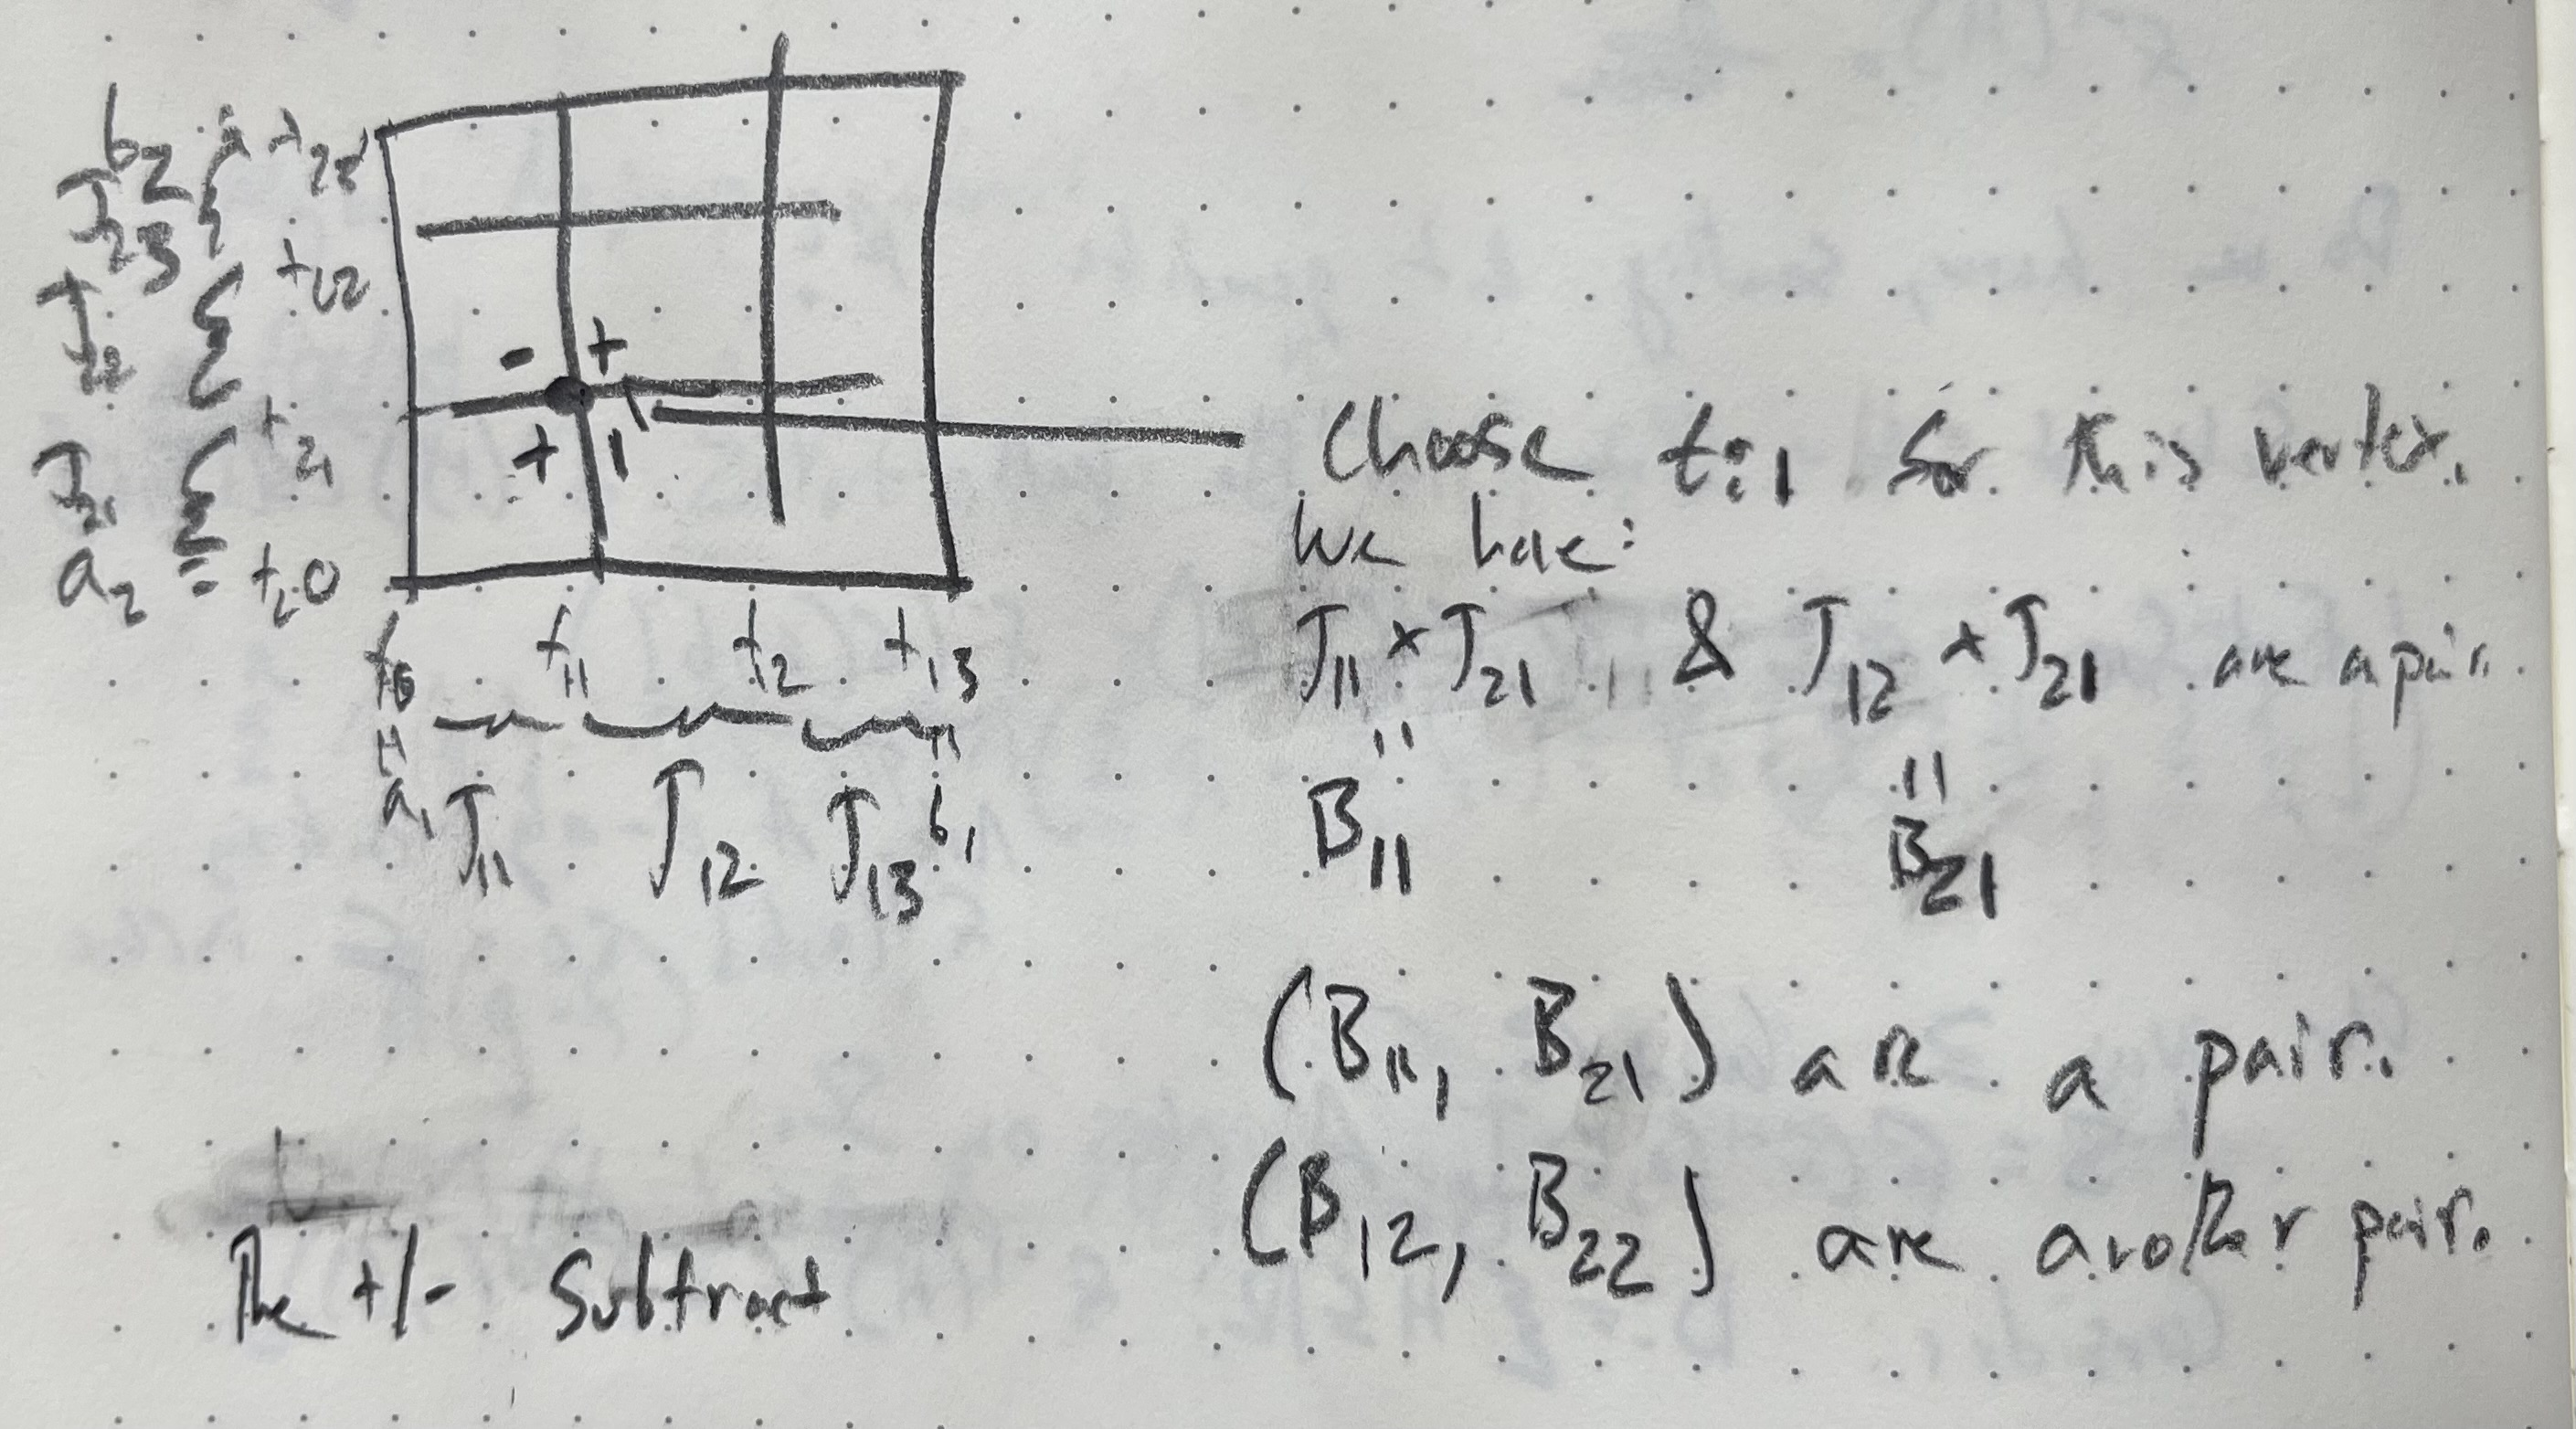
\includegraphics[width=0.7\textwidth]{shared_vertex_rectangles.jpg}
	\caption{Theorem 12.5 Shared Vertex Rectangles}
	\label{fig:example2}
\end{figure} 
So, yeah, each $B$ with a vertex on $x$ has a pair along the $i$ axis, corresponding to whether or not $x_i = t_{ij}$ is an upper bound or lower bound in that dimension. Note:
$$
	\sgn_{B'} x = - \sgn_{B''} x
$$
As for why this is - note all the other intervals are the same. Ie, we have something like:
$$
	J_{1j_1} \times \cdots \times J_{ij} \times \cdots \times J_{kj_k} \quad\text{ vs }\quad
	J_{1j_1} \times \cdots \times J_{i,j+1} \times \cdots \times J_{kj_k}
$$
Note, $\sgn x$ is the count related to the rectangle, oh how many coordinates in $x$ are in the lower bound. Note, the $x$ should have the same lower bound count, except in the $J_{ij}$ vs. $J_{i,j+1}$ interval, and so the signs must be negative of each other. Thus, we have the inner sum on the right below is zero if $x$ is on the interior:
$$
	= \sum_x F(x) \sum_{B} \sgn_B x
$$
So, now we consider the vertices $x$ that are not in the interior - ie, shared by $A$. For those vertices, we have that $x$ is the vertex of only one of the $B$ as well. Further, it is clear that the $\sgn_B x = \sgn_A x$ - you can think of this visually, with the $B$ lining up in the corner of $A$, and $x$ having the same count of $x_i$ being a lower bound for $B$ and $A$. Thus, we have:
$$
	\sum_{j_1,\cdots,j_j} \mu(B_{j_1,\cdots,j_k}) = 
	\sum_{x \in A} F(x) \sgn_B x =
	\sum_{x \in A} \sgn_A x F(x) = \mu(A)
$$
And so, we have countable additivity across regular partitions of a bounded rectangle $A$. Now, suppose that $A = \bigcup_{u=1}^n A_u$, where $A$ is a bounded rectangle, which has the form of a Cartesian product:
$$
	A = I_1 \times \cdots \times I_k
$$
We also have:
$$
	A_u = I_{1u} \times \cdots I_{ku}
$$
Across the $k$ dimensions. Assume the $A_u$ are disjoint. For each $1 \leq i \leq k$, the intervals $I_{i1}, \cdots, I_{in}$ must equal $I_i$. We want to show countable additivity. The overall idea will be - to break up each $A_u$ in such a way, that each $A_u$ has a regular partition, and the union of these regular partitions forms a regular partition of $A$. And then, we can just use additivity of regular partitions to find additivity.
\\\\
Note, each $I_i$ is split up by the endpoints of $I_{iu}$. We have $I_i$ is partitioned by disjoint subintervals $J_{i1}, \cdots, J_{in_i}$, such that each $I_{iu}$ is the union of certain of the $J_{ij}$. Easy enough! Look at the picture in the book for understanding, it is really helpful. The rectangles $B$ of the form:
$$
	B_{j_1,\cdots,j_k} = J_{1j_1} \times \cdots \times J_{kj_k}
$$
Form a regular partition of $A$ - this is clear. Furthermore, the $B$'s contained in a single $A_u$ form a regular partition of $A_u$. As the $A_u$ are disjoint, we have:
$$
	\mu(A) = \sum_B \mu(B) =
	\sum_{u=1}^n \sum_{B \subset A_u} \mu(B) =
	\sum_{u=1}^n \mu(A_u)
$$
Therefore, our $\mu$ is finitely additive on the class $\ical^k$ of bounded $k$-dimensional rectangles.
\\\\
As noted initially - and as in Example 11.4 - $\ical^k$ is a semiring. And so, Theorem 11.3 can apply. So we now work on countable additivity. If $A_,A_1,\cdots,A_n$ are sets in $\ical^k$, then by Lemma 11.2 of the preceding section, we have:
$$
	A \subseteq \bigcup_{u=1}^n A_u \implies
	\mu(A) \leq \sum_{u=1}^n \mu(A_u)
$$
So, we have finite subadditivity on $\ical^k$. Suppose then that $A \subseteq \bigcup_{u=1}^\infty A_u$. We want to extend to/show countable subadditivity:
$$
	\mu(A) \leq \sum_{u=1}^\infty \mu(A_u)
$$
Suppose that $\epsilon > 0$. Take the definition of bounded rectangle $A$ as:
$$
	A = \left[x: a_i < x_i \leq b_i : i = 1, \cdots, k\right]
$$
Now, define:
$$
	B = \left[x: a_i + \delta < x_i \leq b_i : i = 1, \cdots, k\right]
$$
Note, we assume that $a_i < b_i$ for this to work with $\delta$ small enough - and note, that is fine, because if $a_i = b_i$, then we immediately have $\mu(A) = 0$ via cancellations on $\Delta_A F$, and countable subadditivity is thus immediate as well. Note for $\delta$ small enough, we have:
$$
	\mu(A) - \epsilon < \mu(B)
$$
This is because $F$ is continuous from above, so take any $\delta$ approaching zero, and we have $\lim \mu(B_\delta) = \mu(A)$. Also, we have that $\mu(B) < \mu(A)$, via finite additivity. Note that $A$ contains $B$, and the closure of $B$:
$$
	\overline{B} = \left[x: a_i + \delta \leq x_i \leq b_i : i = 1, \cdots, k\right]
$$
Similarly, for each $u$ there is an $\ical^k$ a set:
$$
	B_u = \left[x: a_{iu} < x_i \leq b_{iu} + \delta_u : i = 1, \cdots, k\right]
$$
Such that:
$$
	\mu(B_u) < \mu(A_u) + \epsilon/2^u
$$
And $A_u$ is in the interior of $B_u$:
$$
	\mathring{B_u} = \left[x: a_{iu} < x_i < b_{iu} + \delta_u : i = 1, \cdots, k\right]
$$
And so, in total, we have:
$$
	\overline{B} \subset A \subseteq \bigcup_{u=1}^\infty A_u \subseteq \bigcup_{u=1}^\infty \mathring{B_u}
$$
Now, via Heine-Borel, we have closed rectangles are compact, and so every cover by open sets has a finite subcover. And so, there is some $n$ such that:
$$
	B \subset \overline{B} \subseteq \bigcup_{u=1}^n \mathring{B_u} \subset \bigcup_{u=1}^n B_u
$$
Note now, our Lemma 11.2 note applies, and so:
$$
	\mu(A) - \epsilon < \mu(B) \leq \sum_{u=1}^n \mu(B_u) < \sum_{u=1}^\infty \mu(A_u) + \epsilon
$$
As $\epsilon$ is arbitrary, we can take $\epsilon$ to zero, to find:
$$
	\mu(A) \leq \sum_{u=1}^\infty \mu(A_u)
$$
Thus, $\mu$, as defined, is finitely additive and countably subadditive on the semiring $\ical^k$. By Theorem 11.3, $\mu$ extends to a measure on $\rcal^k = \sigma(\ical^k)$. By Theorem 10.3, this measure is unique. Thus, we have proved the theorem. qed.

\subsubsection{Strange Euclidean Sets}
This is an extra section. It just goes over (note, at a very high level) the Banach Tarski theorem. Recall what congruent means - two shapes are the same size and shape. And they can be moved by rotation/reflection/translation to fit on one another. Ie, one can be obtained from the other via a non-singular linear transformation with determinant 1, or a translation. Take $A$ and $B$ are in $\R^k$, such that they can be decomposed into $A_1, \cdots, A_n$ and $B_1, \cdots, B_n$ where $A_i$ and $B_i$ are congruent. $A$ and $B$ are called \textit{congruent by dissection}. If all the pieces of $A_i$ and $B_i$ are borel sets, then of course:
$$
	\lambda_k(A) = \lambda_k(B)
$$
Via additivity, Theorem 12.1, and Theorem 12.2. But if nonmeasurable sets are allowed in the dissections, then something crazy happens. If $k \geq 3$, and if $A$ and $B$ are bounded sets in $\R^k$ and have nonempty interiors, then $A$ and $B$ are congruent by dissection. Ie, we can find nonmeasurable sets that are congruent, and dissect $A$ and $B$ in a disjoint union - even if $A$ and $B$ are completely different.
\\\\
This is usually illustrated this way: it is possible to break a solid ball the size of a pea into finitely many pieces, and then put them back together in such a way (after a congruent transformation) to get a solid ball the size of the sun.
\\\\
Note - the issue is, the pieces are not solids, but an infinite scattering of points - recall, this matches what a non measurable set it, like with Vitali's construction.

\subsection{Problems}
\subsubsection{12.1 Translation Invariant Measures} Suppose that $\mu$ is a measure on $\rcal^1$ that is finite for bounded sets and is translation-invariant: $\mu(A + x) = \mu(A)$. Show that $\mu(A) = a\lambda(A)$ for some $a \geq 0$. Extend to $\R^k$.
\\\\
First, note that length $1$ bounded intervals generate $\rcal^1$. We have that:
$$
	(a,\infty) = \bigcup_{k=1}^\infty (a + k - 1, a + k]
$$
Something similar for $(-\infty,b)$. We found in problem 11.5 that $(a,\infty),(-\infty,b)$ generate $\rcal^1$. And so, we have for $B$ the set of length one intervals, and $C$ the half infinite intervals:
$$
	B \subseteq C \implies
	\sigma(B) \subseteq \sigma(C) = \rcal^1
$$
$$
	C \subseteq \sigma(B) \implies \rcal^1 \subseteq \sigma(B) \implies
	\rcal^1 = \sigma(B)
$$
Now, note that via translation invariance, for every length 1 interval $A \in B$, we have:
$$
	\mu(A) = a
$$
Note that $a\lambda(A)$ is a measure. We have that:
$$
	\mu(A) = a = a * 1 = a\lambda(A)
$$
For all $A \in B$.
\\\\
Note, I tried to make use of Theorem 10.3, but the length 1 intervals are not a $\pi$ system - an intersection could lead to a non length 1 interval. Anyway. Update $B$ to the bounded intervals - that is indeed a $\pi$ system. I think we can still conclude:
$$
	\mu(A) = a\lambda(A)
$$
For $A \in B$. I think - we can conclude Theorem 12.2 for our measure $\mu$ as well. I am going to go over it - but if it does apply to $\mu$ as well, we can note that scaling by $s$ an interval is a linear transformation $T$ with determinant $s$. Which would be helpful. Or, we can conclude that $\mu(0,1/n] = 1/n\mu(0,1]$. And use rational bounded intervals.
\\\\
Note - the rational intervals generate $\rcal^1$. The rational intervals are also a $\pi$ system. So, if $\mu(I) = a\lambda(I)$ for all rational intervals, then we can conclude that $\mu$ and $a\lambda$, as measures, are equal on all of $\rcal^1$ via the uniqueness of extension Theorem 10.3. As noted above, all length $1$ intervals $I = (a,a+1]$ for rational $a$ have the same measure - say $\mu(A) = a = a\lambda(A)$ - by translation invariance. Now, I will note that all intervals $I_n$ of length $1/n$ have measure:
$$
	\mu(I_n) = a/n = a \lambda(I_n)
$$
By translation invariance, we know the intervals:
$$
	(0,1/n], \cdots, (n-1/n,1]
$$
All have the same measure. Via countable additivity, we have:
$$
	n\mu(0,1/n] = \mu(0,1] \implies \mu(0,1/n] = a/n \implies
	\mu(I_n) = a\lambda(I_n)
$$
Now, take any rational interval $A = (p_1/q_1,p_2/q_2]$. Take $n = q_1 * q_2$. We have $p_2q_1 - p_1q_2$ length $1/n$ intervals that partition $A$:
$$
	(p_1q_2/q_1q_2, (p_1q_2 + 1)/q_1q_2], \cdots,
	((p_2q_1-1)/q_1q_2, p_2q_1/q_1q_2]
$$
Via countable additivity, we have:
$$
	\mu(A) = (p_2q_1 - p_1q_2)\mu(0,1/q_1q_2] =
	a * \left[\frac{p_2q_1 - p_1q_2}{q_1q_2}\right] = a \left[\frac{p_2}{q_2} - \frac{p_1}{q_1}\right] = a\lambda(A)
$$
Thus, the equality holds over the rational intervals. Thus, if $\mu$ is a measure on $\rcal^1$ that is finite for bounded sets and is translation invariant, we have:
$$
	\mu(A) = a\lambda(A)
$$
For some $a \geq 0$. We can extend to $\R^k$ via examining rational rectangles. I guess we could use rational squares - we find $a$ by examining $\mu([0,1]^k)$, then we partition $[0,1]^k$ into $n^k$ squares $[0,1/n]^k$. Same overall argument, to get the same overall result.

\subsubsection{12.2 Measure of a Borel Set is Greater than an Interval} Suppose that $A \in \rcal^1$, $\lambda(A) > 0$, and $0 < \theta < 1$. Show that there is a bounded open interval $I$ such that:
$$
	\lambda(A \cap I) \geq \theta \lambda(I)
$$
First, note that we can assume $\lambda(A)$ is finite. This is because the finite case proves the infinite case. Note that $(\R,\rcal^1,\lambda)$ contains no infinite atoms. This is because, we have:
$$
	A \cap [-n,n] \uparrow A \implies
	\lim \lambda(A \cap [-n,n]) = \infty
$$
And so, there must be some subset $A_n = A \cap [-n,n] \subseteq A$ such that $0 < \lambda(A_n) < \infty$. This is because each $\lambda(A_n) < 2n < \infty$. Also, if each was zero, that would contradict the limit. Anyway, if we have provde the finite case, there for chosen $\lambda(A)$ infinite with $\theta$, we have a $A_n$ where $\lambda(A_n)$ is finite, and the finite case proves there is an $I$ such that:
$$
	\lambda(A \cap I) \geq \lambda(A_n \cap I) \geq \theta \lambda(I)
$$
So now, we assume $A$ is finite, and try and prove the statement. We can find an open $G$ such that:
$$
	A \subset G \text{ and } \lambda(A) \geq \theta\lambda(G)
$$
First note Theorem 12.3 - as $\lambda$ is a measure on $\rcal^1$ that is finite if $A \in \rcal^1$ is bounded, we have for $A \in \rcal^1$ and any $\epsilon > 0$, there is an open set $G$ such that $A \subseteq G$ and:
$$
	\lambda(G - A) < \epsilon
$$
Note - if $\lambda(A) < \infty$, we have $\lambda(G) = \lambda(A) + \lambda(G - A) < \lambda(A) + \epsilon < \infty$. So, we can break up the subtraction - for any $\epsilon$, we can find an open $G$ such that:
$$
	\lambda(G) - \lambda(A) < \epsilon \implies
	\lambda(A) > \lambda(G) - \epsilon
$$
Choose $\epsilon$ small enough such that $\lambda(G) - \epsilon > \theta\lambda(G)$, which is possible as $0 < \theta < 1$. And so, we can indeed conclude that there is an open $G$ such that:
$$
	A \subset G \text{ and } \lambda(A) \geq \theta\lambda(G)
$$
Now, we note that every open set can be written as a disjoint union of open intervals $I_n$:
$$
	G = \bigcup_n I_n
$$
We always go over this proof - write two points in $G$ are in the same equivalence class if they are in an interval contained within $G$. There are only countably many such intervals, as each one contains a rational. Note that via countable additivity and $A \subseteq G \implies A \cap G = A$:
$$
	\sum_n \lambda\left[A \cap I_n\right] =
	\lambda\left[A \cap \bigcup_n I_n\right] =
	\lambda(A) \geq \theta\lambda\left[\bigcup_n I_n\right] =
	\theta\sum_n \lambda(I_n)
$$
Note, if for each $I_n$, we have $\lambda(A \cap I_n) < \theta \lambda(I_n)$, then the above inequality would be contradicted. Thus, there is an $I_n$ such that:
$$
	\lambda(A \cap I_n) \geq \theta \lambda(I_n)
$$
We have thus shown that for $A \in \rcal^1$, $\lambda(A) > 0$, and $0 < \theta < 1$, there is a bounded (each $I_n$ must be bounded, or $G$ would have infinite measure) open interval $I$ such that:
$$
	\lambda(A \cap I) \geq \theta \lambda(I)
$$
qed.

\subsubsection{12.3 Difference Set of a Positive Measure Borel Set Contains the Origin} If $A \in \rcal^1$ and $\lambda(A) > 0$, then the origin is interior to the difference set:
$$
	D(A) = \left[x - y: x,y \in A\right]
$$
I guess - this is kind of a density thing to me. The origin being in the \textit{interior} of the difference set implies that it has an interval around it - so, we have at least one set of points in $A$ that kind of has the thickness of an interval.
\\\\
Take $A \in \rcal^1$ such that $\lambda(A) > 0$. For $\theta = 3/4$, by the above problem 12.2, there is a bounded open interval $I$ such that:
$$
	\lambda(A \cap I) \geq \theta\lambda(I)
$$
Suppose that $|z| < \lambda(I)/2$. Note that both $A \cap I$ and $(A \cap I) + z$ are contained in an interval of length less than $3\lambda(I)/2$. This is because both are contained within $I \cup (I + \lambda(I)/2)$. Thus, the two sets cannot be disjoint, as both sets satisfy:
$$
	\lambda(A \cap I) \geq \frac{3}{4}\lambda(I) \quad\quad\quad
	\lambda(A \cap I + z) \geq \frac{3}{4}\lambda(I)
$$ 
And disjoint would imply $\lambda((A \cap I) \cup (A \cap I) + z) \geq 3\lambda(I)/2$, which would contradict $\lambda((A \cap I) \cup (A \cap I) + z) < 3\lambda(I)/2$. So, there is some $x \in A \cap I$ such that $x \in (A \cap I) + z$, which implies $y = x - z \in A \cap I$. Thus, we have:
$$
	x - y = x - x + z = z \in D(A)
$$
And this is true for all $|z| < \lambda(I)/2$, which does imply zero has an interval around it in $D(A)$, which implies zero is in the interior of the difference set. qed.

\subsubsection{12.4 Extreme NonMeasurable Sets in $\rcal$} The following constructions leads to a subset $H$ of the unit interval that is nonmeasurable in the extreme sense that its inner and outer Lebesgue measures are $0$ and $1$: $\lambda_*(H) = 0$ while $\lambda^*(H) = 1$. I will be filling in the details. The ideas are similar to the construction of the Vitali set. It will be convenient to work in $G = [0,1)$ - let $\oplus$ and $\ominus$ denote addition and subtraction modulo $1$ in $G$, which is a group with identity zero.

\begin{enumerate}
	\item Fix an irrational $\theta$ in $G$ and for $n = 0, \pm 1, \pm 2, \cdots$ let $\theta_n$ be $n\theta$ reduced modulo $1$. Show that $\theta_n \oplus \theta_m = \theta_{n + m}, \theta_n \ominus \theta_m = \theta_{n-m}$, and the $\theta_n$ are distinct. Show that $\left\{\theta_{2n} : n = 0, \pm 1, \cdots\right\}$ and $\left\{\theta_{2n + 1} : n = 0, \pm 1, \cdots\right\}$ are dense in $G$.
	\\\\
	So, we have a lot of stuff to prove. First, I will tackle $\theta_n \oplus \theta_m = \theta_{n + m}$. This is essentially proving something like mod addition is additive. We have:
	$$
		n\theta = b_n + r_n \quad\quad\quad
		m\theta = b_m + r_m
	$$
	For some $b_n,r_m \in \Z$, and $r_n,r_m \in [0,1]$. And so, we have:
	$$
		(n + m)\theta = n\theta + m\theta = (b_n + b_m) + (r_n + r_m)
	$$
	And so now, we have:
	$$
		\theta_{n + m} = (n + m)\theta \mod 1 = (b_n + b_m) + (r_n + r_m) \mod 1 = (r_n + r_m) \mod 1
	$$
	This is clear, as $(b_n + b_m)$ is an integer. Now, note that:
	$$
		\theta_n \oplus \theta_m = (r_n + r_m) \mod 1
	$$
	And so, both sides are equal. We similarly have $\theta_n \ominus \theta_m = \theta_{n-m}$. Now, we want to find that the $\theta_n$ are distinct. Assume for $n \neq m$, we have:
	$$
		\theta_n = \theta_m \implies
		(n\theta \mod 1) = (m\theta \mod 1)
	$$
	This implies that:
	$$
		n\theta = b_n + r_n \quad\quad\quad m\theta = b_m + r_m
	$$
	For $b_n,b_m \in \Z$ and $r_n,r_m \in [0,1)$ and $r_n = r_m$. This implies:
	$$
		n\theta - m\theta = b_n - b_m \implies
		\theta = \frac{b_n - b_m}{n - m}
	$$
	Which would imply $\theta$ is rational, which would be a contradiction. And so, each $\theta_n$ must be distinct. Finally, we want to show that both:
	$$
		\left\{\theta_{2n} : n = 0, \pm 1, \cdots\right\} \quad\quad\text{ and }\quad\quad
		\left\{\theta_{2n + 1} : n = 0, \pm 1, \cdots\right\}
	$$
	Are dense in $G$. Recall, this means that for every $x \in G$, and every open interval containing $x$ in $G$, a member of both sets is in that interval. More simply, every open interval in $G$ has a nonzero intersection with the two sets above. Take $I = (a,b)$. We can restrict $a$ and $b$ to be rational - that is because, there is a rational interval contained within every interval, as the rationals are dense, and so if the sets meet the rational interval, they meet the bigger interval containing the rational interval as well. So:
	$$
		I = \left(\frac{p_1}{q_1}, \frac{p_2}{q_2}\right)
	$$
	Also, I think we can maybe prove for $\theta$ rational first - as we have that the rationals are dense, and we can take a rational close enough to our irrational. Prove something like that. Actually no, I think the rationals might repeat, because for $a/b$, we have $a(b + a)/b = ab/b + a/b = a + a/b$, for which $\mod 1$ would be $a/b$. 
	\\\\
	Maybe consider it like this. Assume that your set hits:
	$$
		(0, 1/n]
	$$
	Then, your set must also hit:
	$$
		(1/n,2/n], \cdots, (n-1/n,n/n]
	$$
	As we can just take $\theta_m \in (0,1/n]$, and multiply it by $2,3,4,\cdots,n$ (as $\theta_{km} = \theta_m \oplus \cdots \oplus \theta_m$, which becomes normal plus as $\theta_m$ is a remainder within $(0,1/n]$). If I can show something similar - that being within $(k/n,k+1/n]$ implies within each of the other sets (mod 1), then I think we are there - as we can just take $n$ arbitrarily large, partition $(0,1]$ such that one of the sets is in $I$.
	\\\\
	Let's try this. Split $G$ into finitely many intervals of length less than $\epsilon > 0$ - one of them must contain points $\theta_{2n}$ and $\theta_{2m}$, with $\theta_{2n} < \theta_{2m}$. This is because each $\theta_n$ is distinct, and so we are putting an infinite amount of points into a finite number of intervals. If the number of intervals is $k$, consider $\theta_{2 * 1}, \cdots, \theta_{2 * 2k}$.
	\\\\
	If $k = m - n$, then $0 < \theta_{2m} - \theta_{2n} = \theta_{2m} \ominus \theta_{2n} = \theta_{2k} < \epsilon$. First step is obvious, second step is because the subtraction is entirely within $[0,1]$, and third step is because they share an interval. The points $\theta_{2kl}$ for $1 \leq l \leq \floor{\theta_{2k}^{-1}}$ form a chain - in which the distance from each to the next is less than $\epsilon$, the first is to the left of $\epsilon$, and the last is to the right of $1 - \epsilon$.
	\\\\
	Ahhh! This is essentially what I wanted to prove above - for each irrational, we have a $\theta_{2k}$ between $(0,1/n]$ - and so, there is a $2kl$ inside of each of the intervals: 
	$$
		(0, 1/n], (1/n,2/n], \cdots, (n-1/n,n/n]
	$$
	Clearly, that implies there is a $\theta_{2kl}$ inside of \textit{any} interval $I$. This proves the first set is dense, and the second set is clearly dense via a similar argument as well.
	
	\item Take $x$ and $y$ to be equivalent if $x \ominus y$ lies in $\left\{\theta_n: n = 0, \pm 1, \cdots\right\}$, which is a subgroup of $G$. Note - $G$ is a group w/ $\oplus$, with associativity clear, identity $0$, and inverse element negative $y = 1 - x \in G$. And by the above, $\oplus$ stays inside of $\left\{\theta_n: n = 0, \pm 1, \cdots\right\}$, $0$ is in the set, and the inverse would just be $\theta_{-n}$, as $\theta_{-n} + \theta_n = \theta_{-n + n} = \theta_0 = 0$.
	\\\\
	Let $S$ contain one representative from each equivalence class (each irrational defines an equivalence class with a countable number of other irrationals). Show that:
	$$
		G = \bigcup_n (S \oplus \theta_n)
	$$
	Where the union is disjoint. Put:
	$$
		H = \bigcup_n (S \oplus \theta_{2n})
	$$
	And show that:
	$$
		G - H = H \oplus \theta
	$$
	\textbf{Problem Start}: Note, it is clear that $\bigcup_n (S \oplus \theta_n)$ is a disjoint union. Take $x \in (S \oplus \theta_n)$ and $x \in (S \oplus \theta_m)$. Note, as adding $\theta_n$ stays inside the subgroup - we have that $x = \theta_k \oplus \theta_n = \theta_{k + n}$ and $x = \theta_k + \theta_m = \theta_{k + m}$ for some irrational $\theta$. Thus, we must have $\theta_{k + m} = \theta_{k + n} \implies m = n$, which is a contradiction. So, we have a disjoint union. Now, we want to show this union equals $G$. Clearly, we have:
	$$
		G \supseteq \bigcup_n (S \oplus \theta_n)
	$$
	So, we go the other direction. Take $x \in G$. Assume $x$ is not in the union. So, $x \neq G$ clearly. We have that every interval containing $x$ intersects with some $(S \oplus \theta_n)$. Note - I think the definition $\left\{\theta_n: n = 0, \pm 1, \cdots\right\}$ allows for rational $\theta$ as well - as the multiplication $k\theta$ for irrational $\theta$ would always be rational. Anyway, in this case, I think it is clear that $x \in [x]$, the corresponding equivalence class, and so we get equality.
	\\\\
	Note - still confused by this. I think, perhaps we have that $S$ takes one representative from each coset? These would be sets of the form $g \in G$, $gH = \{g \oplus h : h \in H\}$. The question also includes (each coset) when it mentioned equivalence classes. I think this would allow for rationals. As, if $g$ is rational, and $n = 0$, we have $\theta_0 = 0 \implies g \oplus \theta_0 = g$. And, we fix a single irrational $\theta$. I think this is how it must be done, actually. So, we will pick up from here.
	\\\\
	\textbf{Problem Start 2} Define:
	$$
		AB = \left\{\theta_n: n = 0, \pm 1, \cdots\right\}
	$$
	For some irrational number $\theta$. Recall, $B$ is a subgroup of $G$ - we talked about this above. Define the set:
	$$
		[x] = xB
	$$
	Which is the left coset of the subgroup of $B$. Recall from group theory - left cosets are equivalence classes. This is equal to the equivalence relation:
	$$
		a \sim b \Leftrightarrow a^{-1}b \in B \Leftrightarrow
		(1 - a) \oplus b \in B \Leftrightarrow b \ominus a \in B
	$$
	Which is the statement in the problem (note, both subtractions differ by 1, modulo 1, so we get the equality). So, if we let $S$ take one element from each of the distinct left cosets, we want to show:
	$$
		G = \bigcup_n (S \oplus \theta_n)
	$$
	For a disjoint union. Equality is clear - as we take $x \in G$, note that for some $y \in [x]$, we have $y \in S$, and definitionally, we note that there is some $\theta_n$ such that $x = y \oplus \theta_n$, which implies $x$ is in the union. And so, we just need to show it is a disjoint union. Again, similar argument as when we were doing the problem incorrectly. If not disjoint, there is an $x \in S \oplus \theta_n$ and $x \in S \oplus \theta_m$. As $[x]$ belongs to the same equivalence class, that tells us $x = y \oplus \theta_n = y \oplus \theta_m \implies m = n$. And so, we have that the union is disjoint as well.
	\\\\
	We now move onto the final part of the problem. Define:
	$$
		H = \bigcup_n (S \oplus \theta_{2n})
	$$
	And show that:
	$$
		G - H = H \oplus \theta
	$$
	I think it is similar to showing that $H$ and $H \oplus \theta$ are disjoint, and their union equals $G$. Clearly, their union equals $G$, as:
	$$
		H \cup H \oplus \theta =
		\bigcup_n (S \oplus \theta_{2n}) \cup \bigcup_n (S \oplus \theta_{2n} \oplus \theta) =
		\bigcup_n (S \oplus \theta_{2n}) \cup \bigcup_n (S \oplus \theta_{2n + 1}) =
		\bigcup_n (S \oplus \theta_n) = G
	$$
	And now, we just have to show that they are disjoint. Well, if $x \in H$, and $x \in H \oplus \theta$, then we have:
	$$
		x = y + \theta_{2n} \quad\quad\quad
		x = y + \theta_{2m + 1}
	$$
	Again, this would imply $2n = 2m + 1$. However, this is a contradiction, as for integer $m$ and $n$, this implies an even number equals an odd number, which is not possible. And so, we cannot have an $x$ in both sets, and so they are disjoint. Thus, we can conclude:
	$$
		G - H = H \oplus \theta
	$$
	
	\item Suppose that $A$ is a Borel set contained in $H$. If $\lambda(A) > 0$, then $D(a)$ contains an interval $(0,\epsilon)$; but then some $\theta_{2k + 1}$ lies in $(0,\epsilon) \subset D(A) \subset D(H)$, and so $\theta_{2k + 1} = h_1 - h_2 = h_1 \ominus h_2 = (s_1 \oplus \theta_{2n_1}) \ominus (s_2 \oplus \theta_{2n_2})$ for some $h_1,h_2$ in $H$ and some $s_1,s_2$ in $S$. Deduce that $s_1 = s_2$ and obtain a contradiction. Conclude that $\lambda_*(H) = 0$.
	\\\\
	We have that:
	$$
		s_1 \ominus s_2 = \theta_{2k + 1} \ominus \theta_{2n_1} \oplus \theta_{2n_2} = \theta_{2k+1} \ominus \theta_{2(n_1-n_2)} =
		\theta_{2(k + n_1 - n_2) + 1}
	$$
	This is just via using associativity rules of the group operation. We note that $s_1$ and $s_2$ must be in the same subgroup - as the difference between them is in $B$, ie a multiple of our original irrational. However, as $s_1$ and $s_2$ are both a member of $S$ - which only contains one member from each subgroup - we have that $s_1 = s_2$. Thus, we have:
	$$
		0 = \theta_{2(k + n_1 - n_2) + 1} \implies
		0 = 2(k + n_1 - n_2) + 1
	$$
	This is a contradiction, as we cannot have an odd number equal to zero. And so, our first statement is incorrect. We cannot have a Borel set contained in $H$, with $\lambda(A) > 0$. So, all Borel sets contained in $H$ must satisfy:
	$$
		\lambda(A) = 0
	$$
	Note, this implies:
	$$
		\lambda_*(A) = 0
	$$
	This comes from problem 3.2, where we found for a probability measure $P$ on a field $\fcal_0$, for every subset of $\Omega$:
	$$
		P^*(A) = \inf\left[P(C): A \subset C, C \in \fcal\right]
	$$
	$$
		P_*(A) = \sup\left[P(C): C \subset A, C \in \fcal\right]
	$$
	Note, we can extend the argument to $\lambda$, to find:
	$$
		\lambda^*(A) = \inf\left[\lambda(C): A \subset C, C \in \rcal^1\right]
	$$
	$$
		\lambda_*(A) = \sup\left[\lambda(C): C \subset A, C \in \rcal^1\right]
	$$
	And so, we have $\lambda_*(H) = 0$, as the supremum of a set containing only zeros is zero.
	
	\item Show that $\lambda_*(H \oplus \theta) = 0$ and $\lambda^*(H) = 1$.
	\\\\
	I think it is clear, via translation invariance, that $\lambda_*(H) = \lambda_*(H \oplus \theta) = 0$. At the very least, we can make a similar argument to above. For $\lambda^*(H)$ - note that:
	$$
		\lambda_*(G - H) = \lambda_*(H \oplus \theta) = 0
	$$
	$$
		\implies 1 - \lambda^*((G - H)^c)) = 0 \implies
		\lambda^*((G - H)^c)) = 1 \implies
		\lambda^*(H) = 1
	$$
	This comes from noting that $G - H = H^c$, and so $(G - H)^c = (H^c)^c = H$. 
	
\end{enumerate}

\subsubsection{12.5 Extreme NonMeasurable Sets in $\rcal$ - 2} The construction here gives sets $H_n$ such that $H_n \uparrow G$ and $\lambda_*(H_n) = 0$. If $J_n = G - H_n$, then $J_n \downarrow \emptyset$ and $\lambda^*(J_n) = 1$.
\begin{enumerate}
	\item Let $H_n = \bigcup_{k=-n}^n (S \oplus \theta_k)$, so that $H_n \uparrow G$. show that the sets $H_n \oplus \theta_{(2n + 1)v}$ are disjoint for different $v$.
	\\\\
	So, it is clear $H_n \uparrow G$, and $\lambda_*(H_n) \leq \lambda_*(H) = 0$. We just need to show the disjoint part. Well, note that $H_n \oplus \theta_{(2n_1)v}$ is just sets $S \oplus \theta_k$, for $k = \{-n, \cdots, -1, 0, 1, \cdots, n\} + (2n + 1)v$. For each $v$, this is a different disjoint subset of $k$, (say $k = 1$, then our set looks like $\{n + 1, \cdots, 3n + 1\}$, etc). And so clearly, each $H_n \oplus \theta_{(2n + 1)v}$ is disjoint for different integer $v$.

	\item Suppose that $A$ is a Borel set contained in $H_n$. Show that $A$ and indeed all the $A \oplus \theta_{(2n + 1)v}$ have Lebesgue measure 0. To be honest - I'm just going to use the monotonicity of the outer measure, which just gives all of these sets are subsets of some $H_n$, which has lower measure zero, which transfers to the lower measure, and thus measure, of $A$.
\end{enumerate}

\subsubsection{12.10 $k$ dimensional analogue of Specifying Measures} Before I state the problem, recall that if $\mu$ is a measure on $\rcal^1$ that assigns finite measures to a bounded set, we could define a real finite function $F$ by:
$$
	F(x) = \begin{cases}
	\mu(0,x] & \text{ if $x \geq 0$}\\
	-\mu(x,0] & \text{ if $x \leq 0$}
	\end{cases}
$$
This was continuous from above, and satisfied $\mu(a,b] = F(b) - F(a)$. For a finite $\mu$, we could standardize $F$ with:
$$
	F(x) = \mu(-\infty,x]
$$
This was the cumulative distribution function. This gave rise to Theorem 12.4, which was a special case of Theorem 12.5, which we proved. 12.4 said - if $F$ is a nondecreasing, right-continuous real function on the line, there exists on $\rcal^1$ a unique measure $\mu$ satisfying $\mu(a,b] = F(b) - F(a)$ for all $a$ and $b$. Theorem 12.5 said - if there was a real function $F$ on $\R^k$ that is continuous from above (ie, $x_n \to x$, and each coordinate is nondecreasing) and satisfies $\Delta_AF \geq 0$ for bounded rectangles $A$, then there exists a unique measure $\mu$ on $\rcal^k$ satisfying $\mu(A) = \Delta_AF$ for all bounded rectangles $A$.
\\\\
Now note - $\mu(A) = \Delta_AF$ makes sense, if we take $F(x) = \mu(S_x)$, for the half infinite rectangle $S_x$ that has top vertex at $x \in \R^k$. Then, $\Delta_A F$ subtracts out the other rectangles, giving the correct definition. However, this requires $\mu$ to be finite on half infinite intervals - ie, this is the analogue of $F(x) = \mu(-\infty,x]$. We want the analogue of the other $F(x)$, in $\R^k$. I think this problem gives that analogue.
\\\\
\textbf{Problem Part 1:} Let $I_t$ be $(0,t]$ for $t \geq 0$ and $(t,0]$ for $t \leq 0$, and let $A_x = I_{x_1} \times \cdots \times I_{x_k}$. Let $\varphi(x)$ be $+1$ or $-1$ according as the number of $i$, $1 \leq i \leq k$, for which $x_i < 0$ is even or odd. Show that, if $F(x) = \varphi(x)\mu(A_x)$, then:
$$
	\mu(A) = \Delta_A F
$$
Holds for bounded rectangles $A$.
\\\\
We will go from the right side to the left side. We have:
$$
	\Delta_A F = \sum_x \sgn_A(x) \cdot F(x) =
	\sum_x \sgn_A(x) \varphi(x) \mu(A_x)
$$
Where $x$ are the vertices of $A$. Note, if $A$ is a bounded rectangle, where in each dimension, $a_i < 0$ and $b_i > 0$, this is just the sum of measures of a partition of $A$ around the origin - see the picture:
\begin{center}
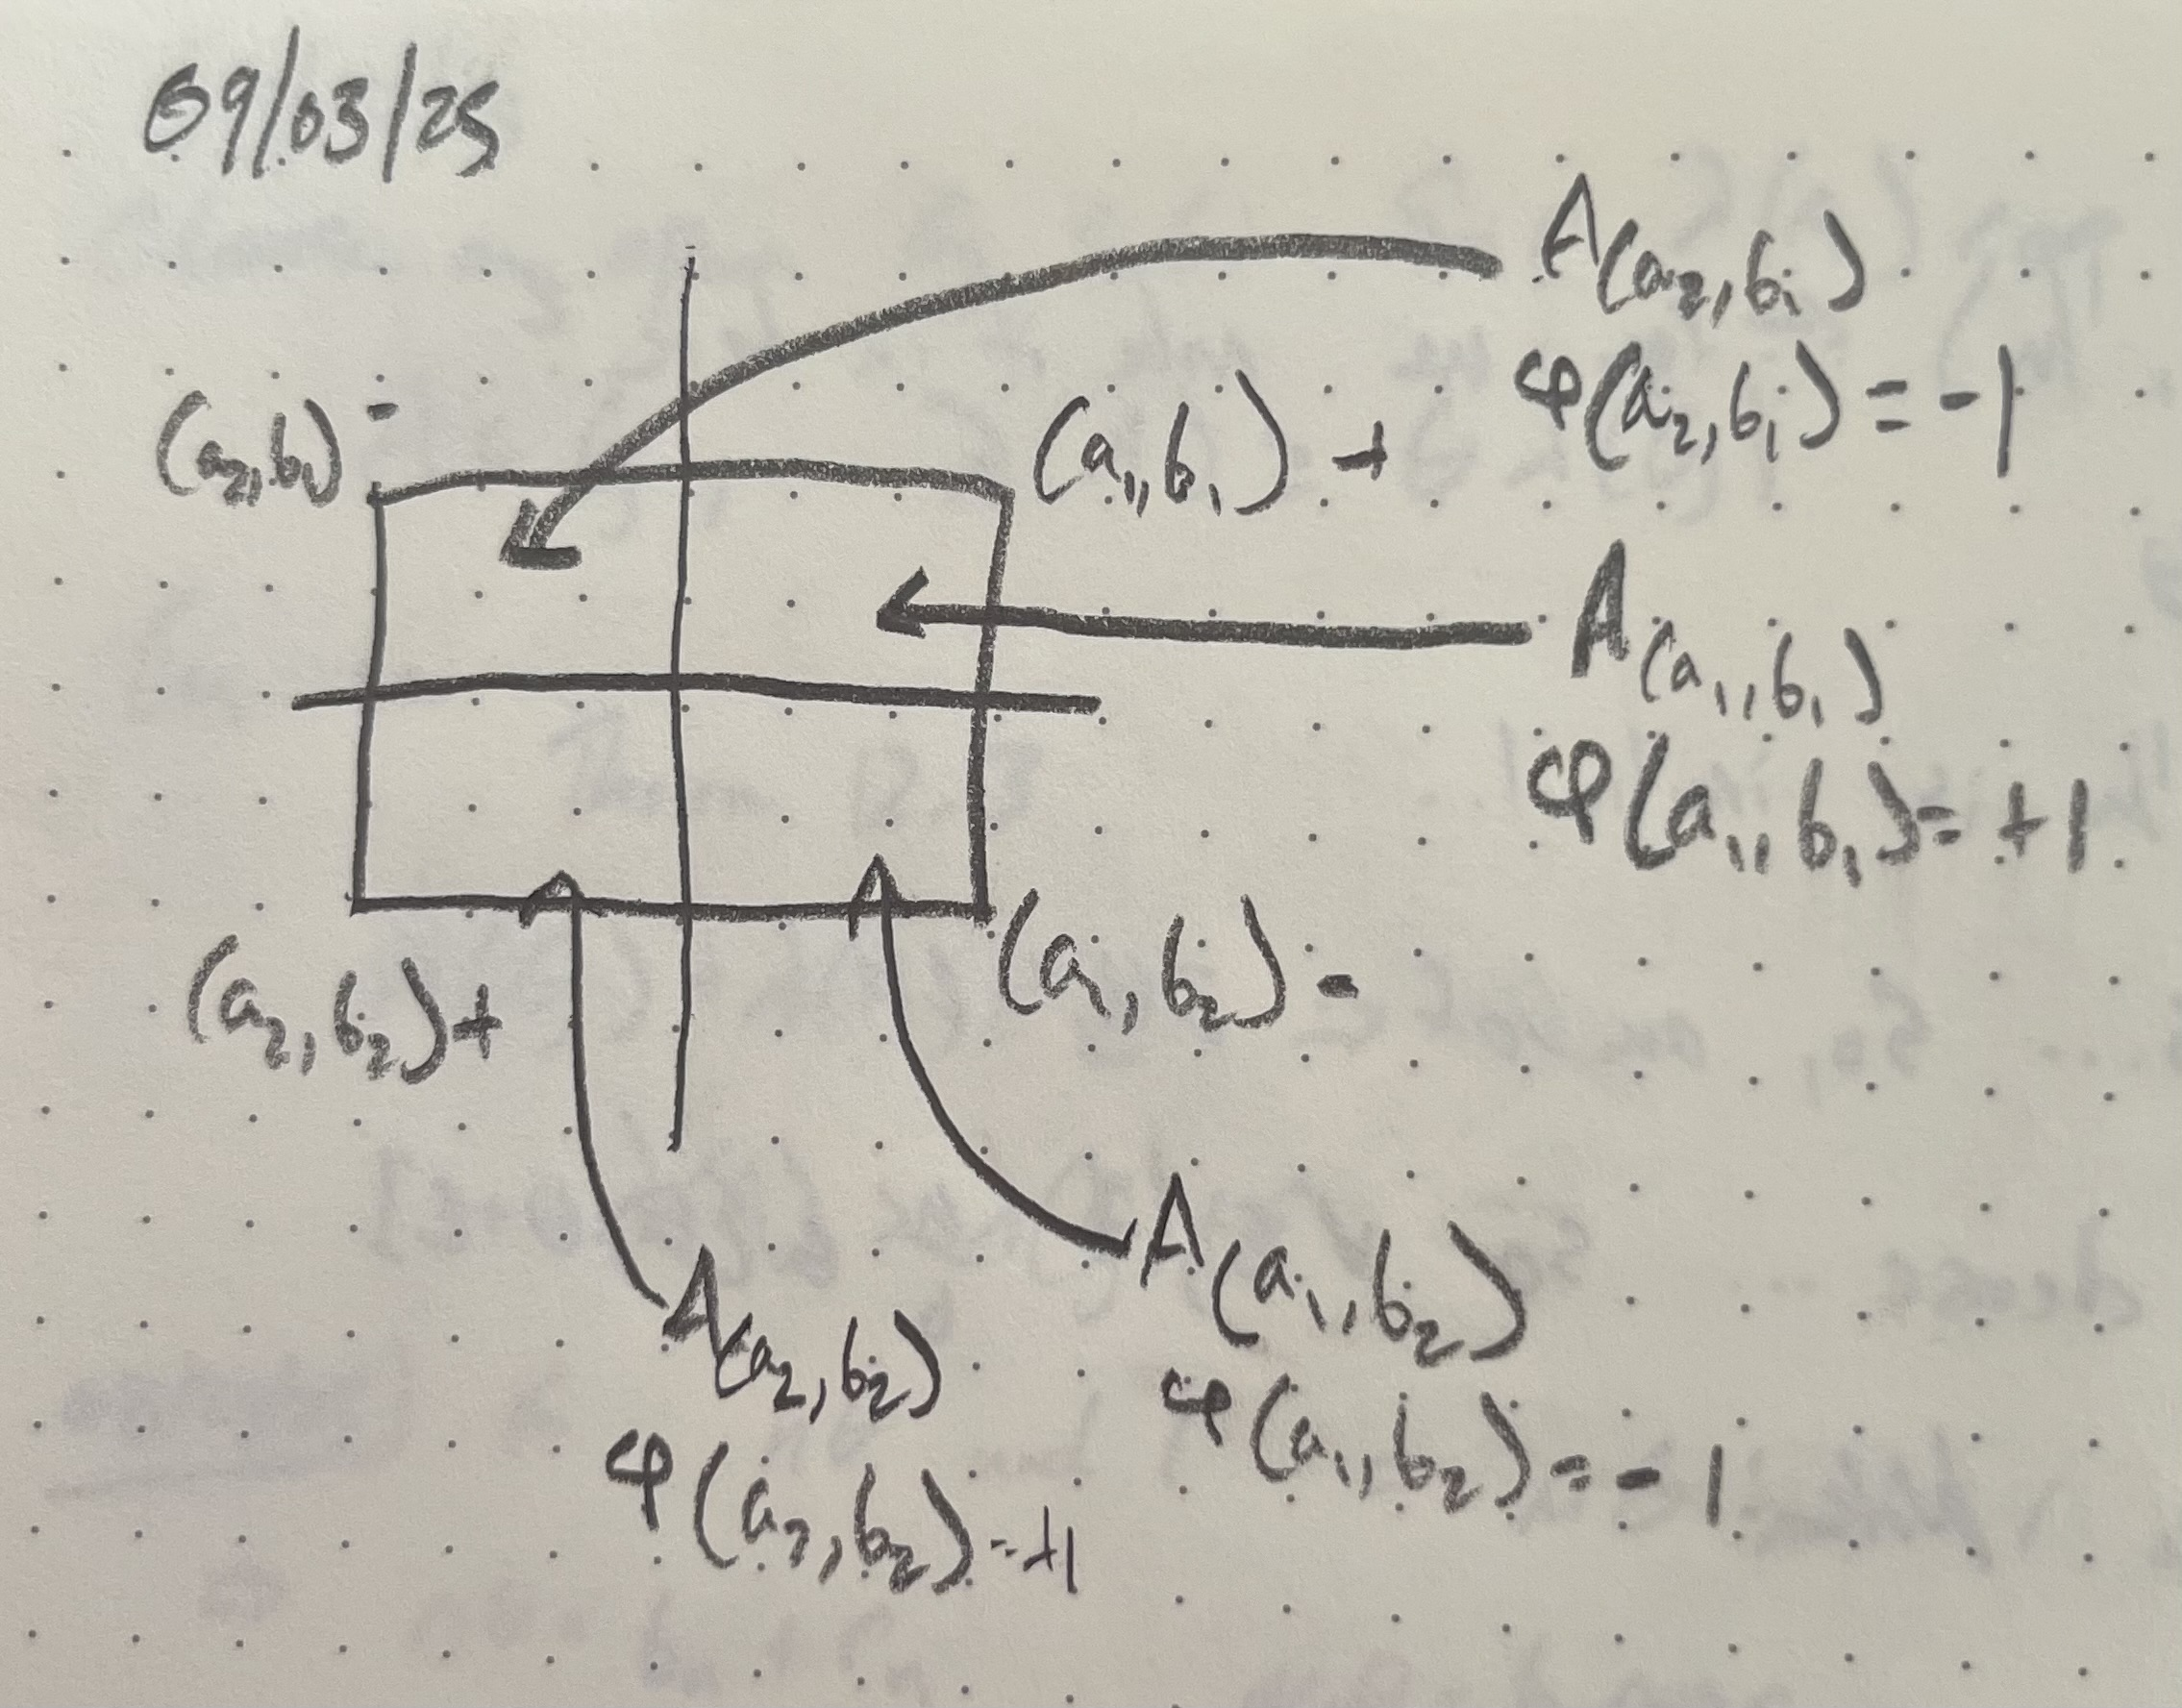
\includegraphics[width=0.8\textwidth]{rec_diff_1.jpg}
\end{center}
The trickier part is if $A$ is a bounded rectangle, and either $0 \leq a_i < b_i$, or $a_i < b_i \leq 0$. However, the cancellations should still work out:
\begin{center}
	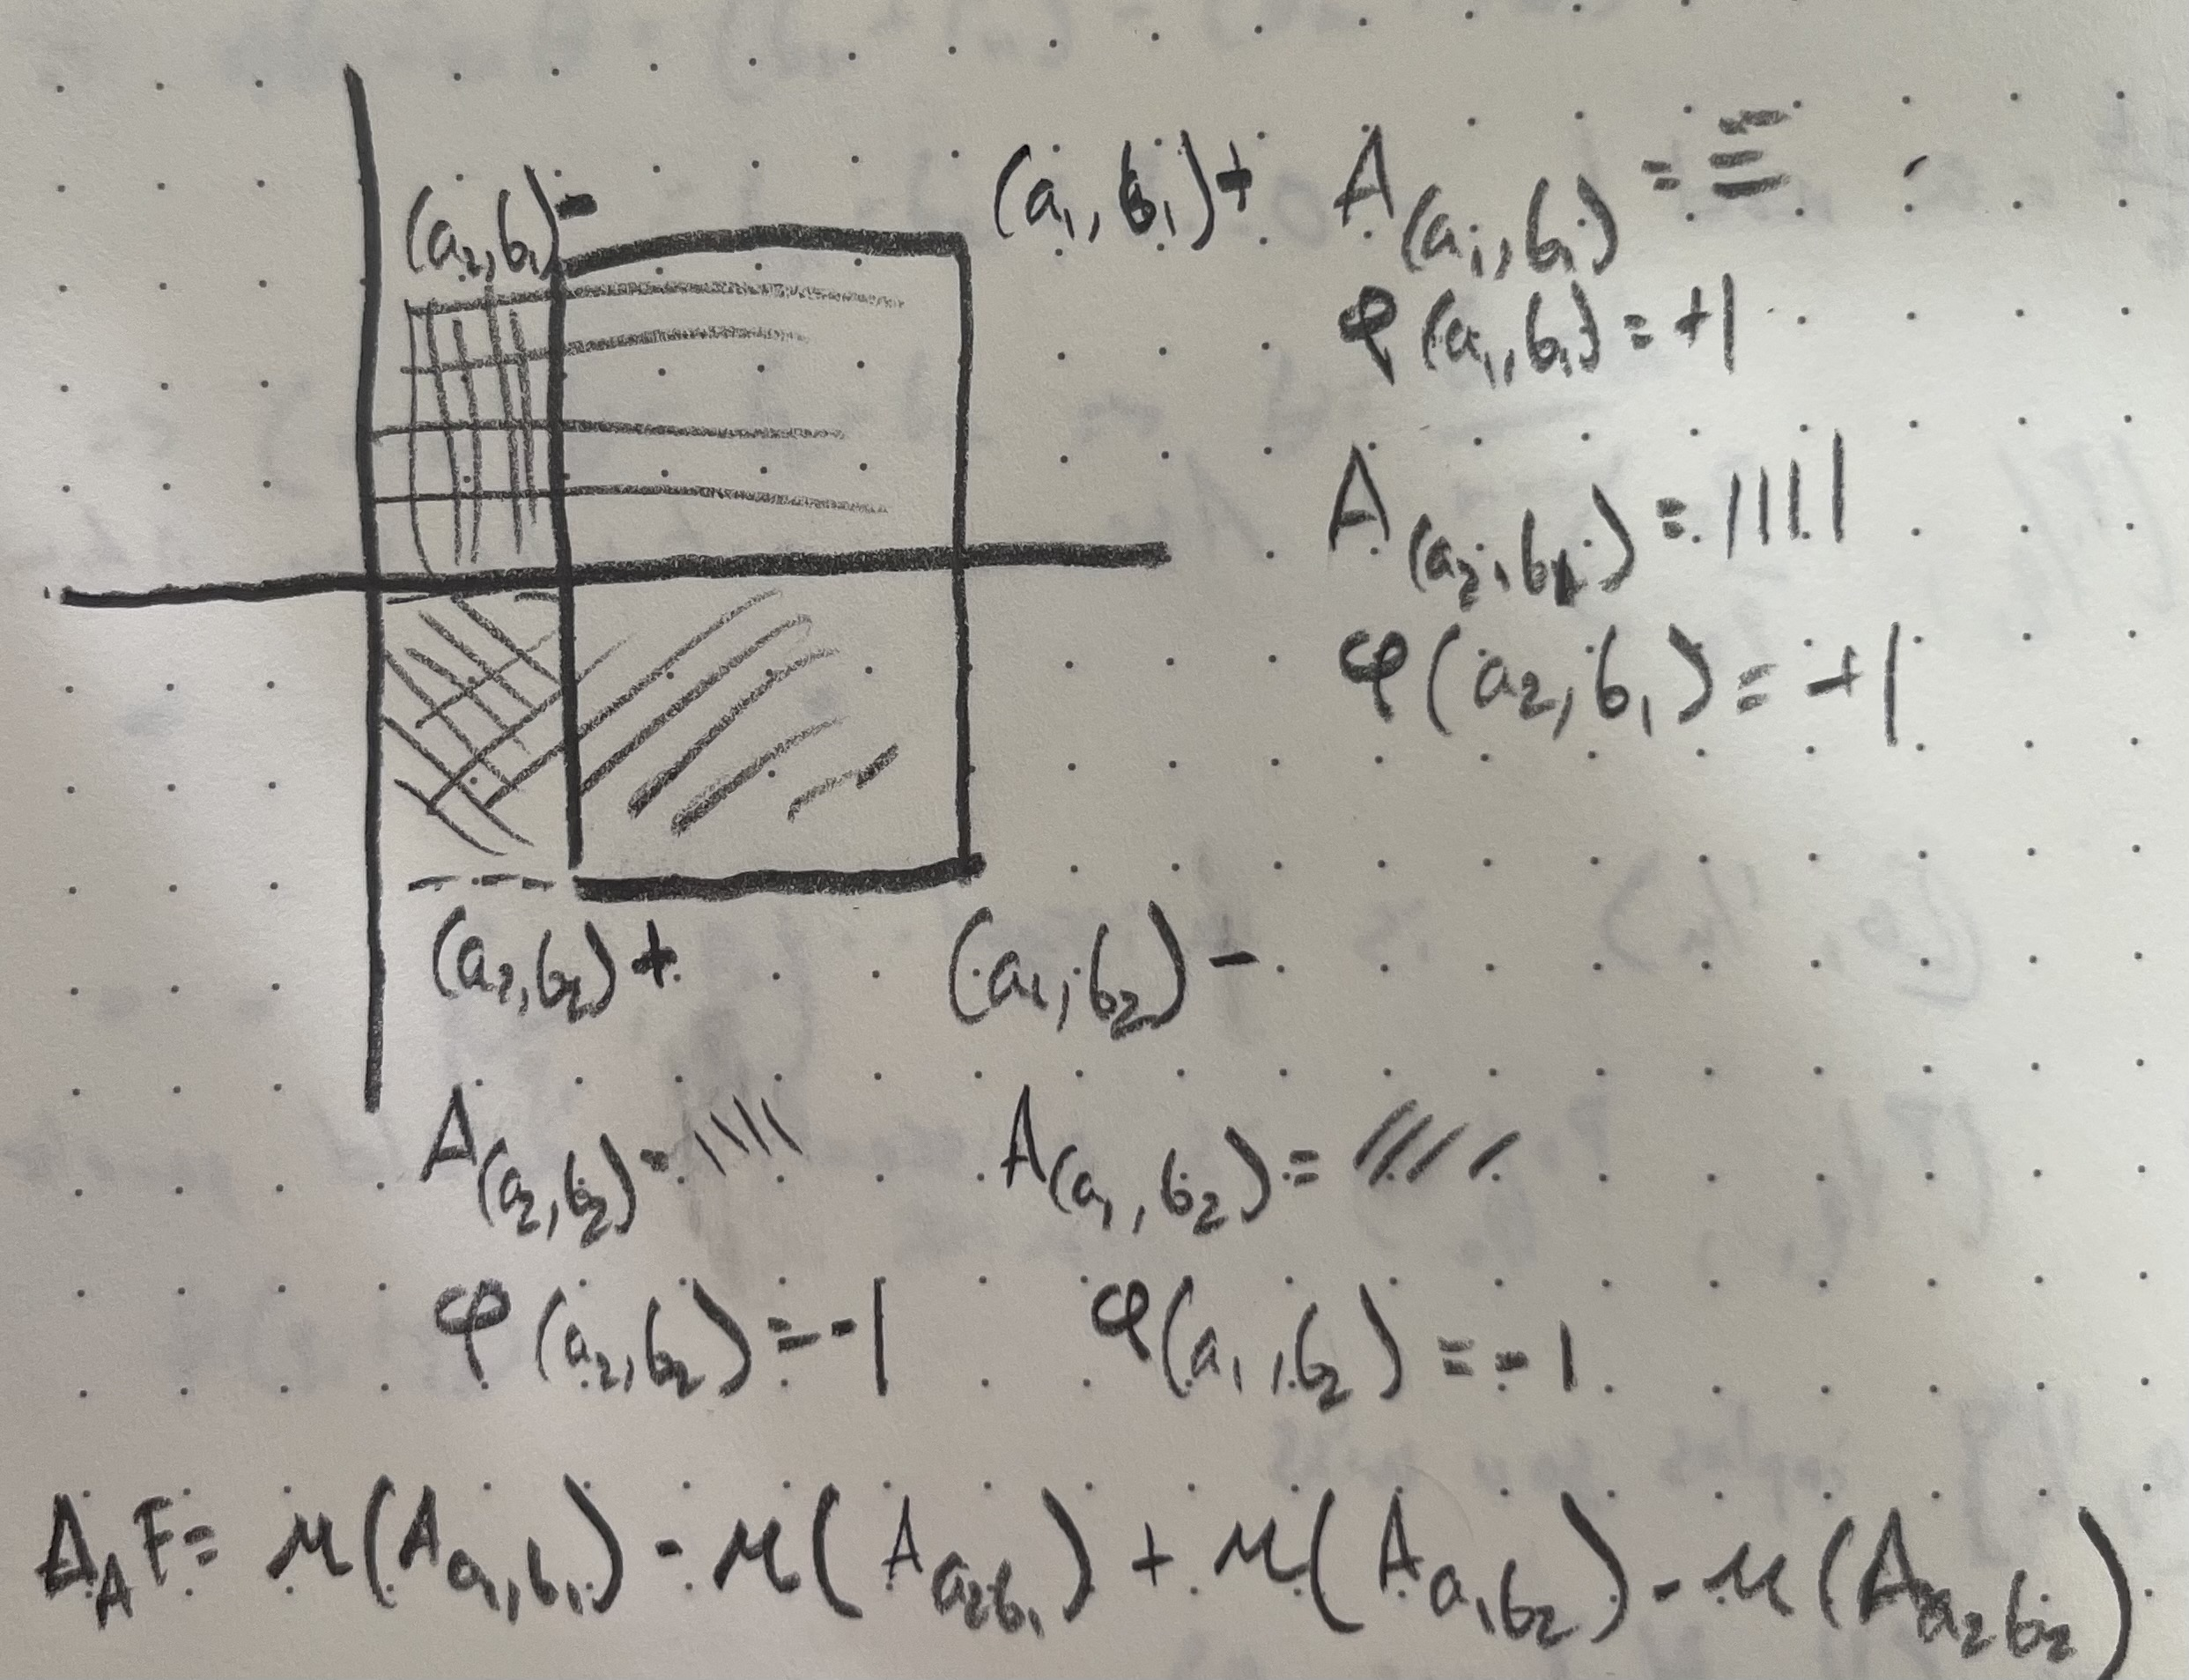
\includegraphics[width=0.8\textwidth]{rec_diff_2.jpg}
\end{center}
I guess the difficult part is generalizing this argument. I think, consider $A = [a_1,b_1] \times \cdots [a_n,b_n]$. Each interval $[a_i,b_i]$ can be expressed as:
$$
	[a_i,b_i] = I_{a_i} \cup I_{b_i} \text{ or } = I_{b_i} - I_{a_i} \text{ or } = I_{a_i} - I_{b_i}
$$
Corresponding to whether or not $a_i,b_i$ are positive and negative, both positive, or both negative. We then consider $2^k$ rectangles
$$
	A_x = I_{x_1} \times \cdots \times I_{x_k}
$$
Where each $x_i$ is either $a_i$ or $b_i$. At a high level - we know, at least via the pictures - there is a partition of the vertices - $P$ and $Q$, such that if $x \in P$, we want to add the measure of $A_x$, and if $x \in Q$, we want to remove the measure of $A_x$, to get the measure of $A$ - something like:
$$
	\mu(A) = \sum_{x \in P} \mu(A_x) - \sum_{x \in Q} \mu(A_x)
$$
the question is - does $\sgn_A(x) \varphi(x)$ being positive imply $x \in P$, and $\sgn_A(x) \varphi(x)$ being negative imply $x \in Q$? Well - consider $A_x$. I think $\sgn_A(x) \varphi(x)$ is positive if $A_x$ intersects with $A$, and negative if it doesn't. This is actually incorrect - I think there is a case where it is positive, and we want to add back a section we double subtracted.
\\\\
I'm going to stick with intuition on this one. Thought about it for a while, couldn't really think of how to prove it rigorously. Other than, maybe going case by case?
\\\\
\textbf{Problem Part 2:} Call $F$ degenerate if it is a function of some $k-1$ of the coordinates, the requirement in the case $k = 1$ being that $F$ is constant. Show that $\Delta_A F = 0$ for every bounded rectangle if and only if $F$ is a finite sum of degenerate functions - $\mu(A) = \Delta_AF$ determines $F$ to within addition of a function of this sort.

\end{document}





















